% Eigenständige deutschsprachige Studienausgabe.
\documentclass[11pt]{article}
\usepackage{fontspec}
\usepackage{amsmath}
\usepackage{unicode-math}
\setmainfont{Noto Serif}
\setsansfont{Noto Sans Display}
\setmonofont[Scale=.87]{DejaVu Sans Mono}
\setmathfont{Latin Modern Math}
\usepackage[paperwidth=183mm,paperheight=250mm,left=18mm,right=18mm,top=22mm,bottom=21mm,headheight=24pt,headsep=8mm,footskip=11mm]{geometry}
\usepackage{graphicx,xcolor,booktabs,tabularx,array,fancyhdr,ragged2e}
\usepackage[unicode,pdfencoding=auto,bookmarksopen=true,bookmarksopenlevel=0,bookmarksnumbered=false,colorlinks=true]{hyperref}
\definecolor{ink}{HTML}{1C343B}
\definecolor{sea}{HTML}{006963}
\definecolor{umber}{HTML}{9E4425}
\definecolor{mute}{HTML}{4D656B}
\definecolor{linegrey}{HTML}{CADAD6}
\definecolor{tint}{HTML}{EFF6F3}
\hypersetup{pdftitle={Numerische Simulation dynamischer Systeme},pdfauthor={Christian Stenzel},pdfsubject={Modellbildung, Systemtheorie und Solverwahl mit ARGESIM-Fallstudien},pdflang={de-DE},linkcolor=sea,urlcolor=sea}
\newcommand{\pubrev}{1824c9104152674b82de6cd84d53b0b4f68dca37}
\newcommand{\repo}[2]{\href{https://github.com/5H3LL3H5/argesim-hyperposition-benchmarks/blob/1824c9104152674b82de6cd84d53b0b4f68dca37/#1}{#2}}
\newcommand{\repocurrent}[2]{\href{https://github.com/5H3LL3H5/argesim-hyperposition-benchmarks/blob/main/#1}{#2}}
\setlength{\parindent}{0pt}
\setlength{\parskip}{4.4pt}
\setlength{\emergencystretch}{1.8em}
\setlength{\tabcolsep}{4.5pt}
\setlength{\jot}{2pt}
\raggedbottom
\newcommand{\running}{Studienausgabe}
\pagestyle{fancy}
\fancyhf{}
\fancyhead[L]{\small\sffamily\color{mute}Numerische Simulation dynamischer Systeme}
\fancyhead[R]{\small\sffamily\color{sea}\running}
\fancyfoot[L]{\footnotesize\sffamily\color{mute}Christian Stenzel\enspace·\enspace Studienausgabe 2026}
\fancyfoot[R]{\sffamily\bfseries\color{sea}\thepage}
\renewcommand{\headrulewidth}{.35pt}
\renewcommand{\headrule}{\hbox to\headwidth{\color{linegrey}\leaders\hrule height \headrulewidth\hfill}}
\newcommand{\anchorpage}[3]{\phantomsection\hypertarget{#2}{}\label{#2}\pdfbookmark[#1]{#3}{bm-#2}}
\newcommand{\ey}[1]{{\sffamily\bfseries\fontsize{9}{11}\selectfont\color{sea}#1\par}}
\newcommand{\ptitle}[1]{{\sffamily\bfseries\color{ink}\fontsize{21.5}{25.5}\selectfont\raggedright\hyphenpenalty=10000\exhyphenpenalty=10000 #1\par}\vspace{3pt}}
\newcommand{\chap}[4]{\clearpage\renewcommand{\running}{#2}\anchorpage{1}{#4}{#1 · #2}\ey{KAPITEL #1\enspace /\enspace #2}\vspace{3pt}\ptitle{#3}}
\newcommand{\unit}[2]{\clearpage\anchorpage{2}{#2}{#1}\ptitle{#1}}
\newcommand{\subt}[1]{\par\vspace{4pt}{\sffamily\bfseries\color{ink}\fontsize{12.2}{15}\selectfont #1\par}\nopagebreak}
\newcommand{\why}[1]{\par{\itshape\color{mute}#1\par}\vspace{2pt}}
\newcommand{\notebox}[2]{\par\vspace{3pt}\begingroup\setlength{\fboxsep}{7pt}\noindent\colorbox{tint}{\begin{minipage}{\dimexpr\linewidth-2\fboxsep\relax}\RaggedRight\fontsize{10}{13.1}\selectfont\textsf{\bfseries\color{sea}#1}\enspace #2\end{minipage}}\endgroup\par}
\newcommand{\proofpart}[1]{\par\textsf{\bfseries\color{sea}Beweis.}\enspace #1\hfill{\color{sea}\rule{4pt}{4pt}}\par}
\newcommand{\capline}[1]{\par\vspace{-1pt}{\sffamily\fontsize{8.45}{11.3}\selectfont\color{mute}#1\par}}
\newcounter{fig}
\newcommand{\minifig}[3]{\par\vspace{2pt}{\centering\includegraphics[height=#2,width=.96\linewidth,keepaspectratio]{#1.pdf}\par}\refstepcounter{fig}\capline{\textbf{Abb. \thefig}\enspace #3}}
\newcommand{\fig}[3]{\par\vspace{3pt}\begin{center}\includegraphics[width=#2\linewidth]{#1.pdf}\end{center}\vspace{-6pt}\refstepcounter{fig}\capline{\textbf{Abb. \thefig}\enspace #3}}
\newcommand{\figsmall}[3]{\fig{#1}{#2}{#3}}
\newcommand{\srcs}[1]{\par\vfill{\sffamily\fontsize{8.1}{10.8}\selectfont\color{mute}#1\par}}
\newcommand{\see}[2]{\hyperlink{#1}{#2, S.\,\pageref*{#1}}}
\newcommand{\pagelink}[1]{\hyperlink{#1}{\pageref*{#1}}}
\newcommand{\task}[2]{\par\hypertarget{aufgabe#1}{}\notebox{Aufgabe #1}{#2 \hyperlink{loes#1}{Lösung}}}
\newcolumntype{Y}{>{\RaggedRight\arraybackslash}X}
\newcolumntype{P}[1]{>{\RaggedRight\arraybackslash}p{#1}}
\newcommand{\tblstart}{\par\noindent\sffamily\fontsize{9.25}{12.2}\selectfont\renewcommand{\arraystretch}{1.17}}
\newcommand{\hd}[1]{\textbf{\color{sea}#1}}
\newcommand{\dg}{\,\mathrm{d}}
\newcommand{\dd}{\mathrm{d}}
\newcommand{\unitm}[1]{\,\mathrm{#1}}
\newcommand{\refbk}[2]{\hyperlink{lit-#1}{#2}}
\newcommand{\zerolist}{\setlength{\topsep}{0pt}\setlength{\itemsep}{1pt}\setlength{\parsep}{0pt}}

\graphicspath{{abbildungen/}}
\hyphenation{ver-glei-chen Re-si-du-al-form Ra-ten Glei-chun-gen erste höchstens re-la-ti-ven lie-fern vie-le Zeit-punkt}
\newcommand{\vorhersage}[3]{\par\begingroup\sffamily\fontsize{9.25}{12.1}\selectfont\color{sea}\hypertarget{frage#1}{}\textbf{Erst schätzen.}\enspace #2\enspace\hyperlink{antwort#1}{\textit{Auflösung S.\,\pageref*{#3}}}\par\endgroup}
\newcommand{\kapschluss}[3]{\clearpage\anchorpage{2}{#3}{Forschungsstand und Beweisfragen · Kapitel #1}\ey{KAPITELABSCHLUSS #1}\vspace{3pt}\ptitle{#2}}
\newcommand{\teilende}[3]{\clearpage\renewcommand{\running}{Abschluss Teil #1}\anchorpage{1}{#3}{Abschluss Teil #1 · Stand und offene Beweise}\ey{ABSCHLUSS TEIL #1}\vspace{3pt}\ptitle{#2}}

\definecolor{goldbg}{HTML}{FCF2E6}
\definecolor{goldink}{HTML}{7B3D19}
\newcommand{\lernziel}[1]{\par{\sffamily\fontsize{9.6}{12.8}\selectfont\textbf{\color{sea}Lernziel}\enspace #1\par}\vspace{3pt}}
\newcommand{\merke}[1]{\notebox{Das Werkzeug}{#1}}
\newcommand{\hilfe}[1]{\par\vspace{4pt}\begingroup\setlength{\fboxsep}{7pt}\noindent\colorbox{goldbg}{\begin{minipage}{\dimexpr\linewidth-2\fboxsep\relax}\RaggedRight\fontsize{9.9}{13.1}\selectfont\textsf{\bfseries\color{goldink}Ein Hinweis}\enspace #1\end{minipage}}\endgroup\par}
\newcommand{\schreibfeld}{\par\vspace{4mm}{\small\sffamily\color{mute}Mein erster Rechenschritt und meine Gegenprobe\par}\vspace{1.8mm}{\color{linegrey}\hrule height .4pt}\vspace{5.5mm}{\color{linegrey}\hrule height .4pt}\par}
\newcommand{\rolle}{}
\newcommand{\seite}[2]{\clearpage\renewcommand{\rolle}{#1}\renewcommand{\running}{#2}}
\newcommand{\lektion}[4]{\seite{#3}{#4}\anchorpage{2}{#2}{#1}\ptitle{#1}}
\newcommand{\werkblatt}[4]{\seite{#2}{Kapitel #1}\anchorpage{2}{#3}{#2 · Kapitel #1}\ey{KAPITEL #1\enspace /\enspace #2}\ptitle{#4}}
\renewcommand{\kapschluss}[3]{\seite{Forschung}{Kapitel #1}\anchorpage{2}{#3}{Forschungsstand und Beweisfragen · Kapitel #1}\ey{KAPITELABSCHLUSS #1}\ptitle{#2}}
\renewcommand{\teilende}[3]{\seite{}{Abschluss Teil #1}\anchorpage{1}{#3}{Abschluss Teil #1 · Stand und offene Beweise}\ey{ABSCHLUSS TEIL #1}\ptitle{#2}}
\fancyhead[R]{{\footnotesize\sffamily\color{mute}\rolle\enspace\color{sea}\running}}
\fancyfoot[L]{\footnotesize\sffamily\color{mute}Christian Stenzel\enspace·\enspace Studienbuch für das Bachelorstudium}

\newcommand{\cpcode}[2]{\href{https://github.com/5H3LL3H5/argesim-hyperposition-benchmarks/blob/52f8a33e469d36514e7830db544b9fc27243a82c/#1}{#2}}
\newcommand{\bilanz}[3]{\seite{}{Rückblick}\anchorpage{2}{#3}{Rückblick · Teil #1}\ey{RÜCKBLICK AUF TEIL #1}\ptitle{#2}}
\begin{document}
\ifcsname l@ngerman\endcsname\language=\csname l@ngerman\endcsname\relax\fi\lefthyphenmin=2\righthyphenmin=2
\color{ink}\RaggedRight\fontsize{10.55}{14.45}\selectfont
\setlength{\abovedisplayskip}{6.5pt}\setlength{\belowdisplayskip}{6.5pt}
\setlength{\abovedisplayshortskip}{3pt}\setlength{\belowdisplayshortskip}{4pt}


\thispagestyle{empty}\anchorpage{0}{titel}{Titel}
\vspace*{4mm}\ey{STUDIENBUCH FÜR DAS BACHELORSTUDIUM}
\vspace{9mm}
{\sffamily\bfseries\fontsize{35}{40}\selectfont\color{ink}Numerische Simulation\\dynamischer Systeme\par}
\vspace{5mm}{\sffamily\fontsize{17}{23}\selectfont\color{sea}Mathematische Fundierung, moderne Solver-Konzepte\\und der ARGESIM-Benchmark-Prüfstand\par}
\vspace{9mm}{\sffamily\fontsize{14}{19}\selectfont Christian Stenzel\par}
\vfill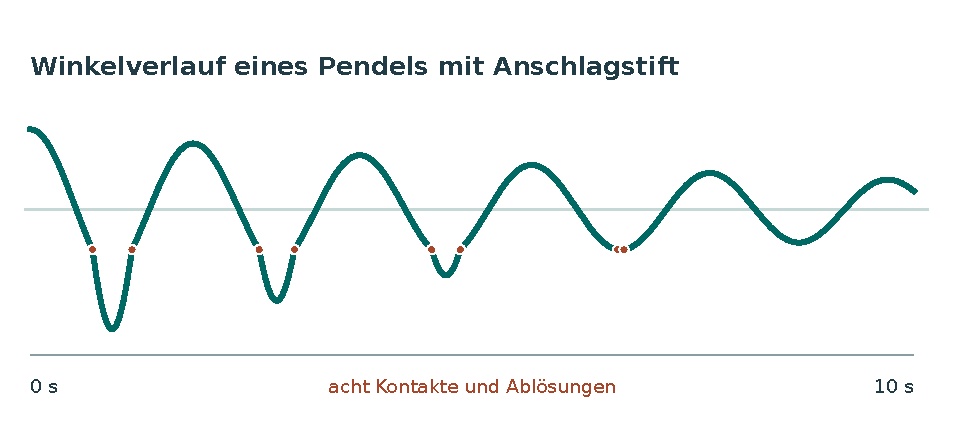
\includegraphics[width=\linewidth]{umschlag.pdf}\vfill
{\color{linegrey}\rule{\linewidth}{.7pt}}\par
{\sffamily\fontsize{10}{13}\selectfont\color{mute}Modellieren, rechnen, Ergebnisse prüfen\hfill November 2026\par}

\seite{}{INHALT}\anchorpage{0}{inhalt}{INHALT · Wie das Buch aufgebaut ist}\ey{INHALT}\ptitle{Wie das Buch aufgebaut ist}
Die Temperatur eines Fühlers, der Zeitpunkt eines Stoßes und das Geschwindigkeitsfeld einer Kavität stellen unterschiedliche Fragen an eine Simulation. Teil I entwickelt das nötige Werkzeug. Teil II prüft es am Modell. Teil III enthält Referenzen, Einzelmessungen und Verträge.
{\tblstart\begin{tabularx}{\linewidth}{@{}Yr@{}}\toprule
\hyperlink{grundteil}{I · Mathematische Fundierung und Solver-Algorithmik} & \pagelink{grundteil}\\[2pt]
\hyperlink{praxisteil}{II · Die didaktischen ARGESIM-Leitbenchmarks} & \pagelink{praxisteil}\\[2pt]
\hyperlink{refteil}{III · ARGESIM-Referenzkatalog} & \pagelink{refteil}\\[2pt]
\hyperlink{anhang}{Aufgaben, Lösungen und Literatur} & \pagelink{anhang}\\[2pt]
\bottomrule\end{tabularx}\par}
\subt{Detailliertes Inhaltsverzeichnis}
{\tblstart\begin{tabularx}{\linewidth}{@{}Yr@{}}\toprule
\hyperlink{toc1}{Kapitel 1 · Dynamische Systeme und Steifigkeit} & \pagelink{toc1}\\[2pt]
\hyperlink{toc2}{Kapitel 2 · Explizite Einschrittverfahren} & \pagelink{toc2}\\[2pt]
\hyperlink{toc3}{Kapitel 3 · Implizite Integratoren} & \pagelink{toc3}\\[2pt]
\hyperlink{toc4}{Kapitel 4 · DAEs und Bindungen} & \pagelink{toc4}\\[2pt]
\hyperlink{toc5}{Kapitel 5 · Hybride Systeme} & \pagelink{toc5}\\[2pt]
\hyperlink{toc6}{Kapitel 6 · QSS und DEVS} & \pagelink{toc6}\\[2pt]
\hyperlink{toc7}{Kapitel 7 · Räumliche Diskretisierung} & \pagelink{toc7}\\[2pt]
\hyperlink{toc8}{Kapitel 8 · Lattice-Boltzmann} & \pagelink{toc8}\\[2pt]
\hyperlink{toc9}{Kapitel 9 · Scientific Machine Learning} & \pagelink{toc9}\\[2pt]
\hyperlink{tocpraxis}{Kapitel 10–17 und die Anhänge} & \pagelink{tocpraxis}\\[2pt]
\bottomrule\end{tabularx}\par}
\seite{Gliederung}{Inhaltsverzeichnis}\anchorpage{1}{toc1}{Kapitel 1 · Dynamische Systeme und Steifigkeit}\ptitle{Kapitel 1 · Dynamische Systeme und Steifigkeit}
\subt{\hyperlink{abs1-1}{1.1 · Kontinuierliche Systeme im Zustandsraum}\hfill S.\,\pagelink{abs1-1}}
\hyperlink{punkt1-1-1}{1.1.1\enspace Vektorfelder, Phasenporträts und Trajektorien}\par
\hyperlink{punkt1-1-2}{1.1.2\enspace Autonome Systeme und die Zeit als Zustand}\par
\hyperlink{punkt1-1-3}{1.1.3\enspace Bilanzen, Erhaltungsgrößen und Hamilton-Systeme}\par
\subt{\hyperlink{abs1-2}{1.2 · Anfangswertprobleme und Solver-Verträge}\hfill S.\,\pagelink{abs1-2}}
\hyperlink{punkt1-2-1}{1.2.1\enspace Existenz und Eindeutigkeit nach Picard und Lindelöf}\par
\hyperlink{punkt1-2-2}{1.2.2\enspace Lipschitz-Bedingung und Konditionierung}\par
\hyperlink{punkt1-2-3}{1.2.3\enspace Ordnungsreduktion in beide Richtungen}\par
\hyperlink{punkt1-2-4}{1.2.4\enspace Zustandsform und Residualform}\par
\subt{\hyperlink{abs1-3}{1.3 · Steifigkeit und die Grenzen eines expliziten Schritts}\hfill S.\,\pagelink{abs1-3}}
\hyperlink{punkt1-3-1}{1.3.1\enspace Zwei thermisch gekoppelte Zonen}\par
\hyperlink{punkt1-3-2}{1.3.2\enspace Dahlquistsche Testgleichung}\par
\hyperlink{punkt1-3-3}{1.3.3\enspace Stabilität und Genauigkeit getrennt prüfen}\par
\srcs{\see{neu1}{Kapitel lesen} · \see{inhalt}{Zur Übersicht}.}
\seite{Gliederung}{Inhaltsverzeichnis}\anchorpage{1}{toc2}{Kapitel 2 · Explizite Einschrittverfahren}\ptitle{Kapitel 2 · Explizite Einschrittverfahren}
\subt{\hyperlink{abs2-1}{2.1 · Runge–Kutta-Verfahren konstruieren}\hfill S.\,\pagelink{abs2-1}}
\hyperlink{punkt2-1-1}{2.1.1\enspace Zwischenstufen als vorläufige Zustände}\par
\hyperlink{punkt2-1-2}{2.1.2\enspace Butcher-Tableau und Ordnungsbedingungen}\par
\hyperlink{punkt2-1-3}{2.1.3\enspace Heun, Kutta dritter Ordnung und klassisches RK4}\par
\subt{\hyperlink{abs2-2}{2.2 · Lokaler Fehler und eingebettete Paare}\hfill S.\,\pagelink{abs2-2}}
\hyperlink{punkt2-2-1}{2.2.1\enspace Vom lokalen Defekt zum globalen Fehler}\par
\hyperlink{punkt2-2-2}{2.2.2\enspace Zwei Endwerte aus denselben Stufen}\par
\hyperlink{punkt2-2-3}{2.2.3\enspace RK23, RK45 und DOP853 unterscheiden}\par
\subt{\hyperlink{abs2-3}{2.3 · Schrittweitensteuerung und dichte Ausgabe}\hfill S.\,\pagelink{abs2-3}}
\hyperlink{punkt2-3-1}{2.3.1\enspace Relative und absolute Fehlerskalen}\par
\hyperlink{punkt2-3-2}{2.3.2\enspace I-, PI- und PID-Regelung}\par
\hyperlink{punkt2-3-3}{2.3.3\enspace Akzeptanz, Verwerfung und Grenzen}\par
\hyperlink{punkt2-3-4}{2.3.4\enspace Hermite- und Kollokationspolynome}\par
\srcs{\see{neu2}{Kapitel lesen} · \see{inhalt}{Zur Übersicht}.}
\seite{Gliederung}{Inhaltsverzeichnis}\anchorpage{1}{toc3}{Kapitel 3 · Implizite Integratoren}\ptitle{Kapitel 3 · Implizite Integratoren}
\subt{\hyperlink{abs3-1}{3.1 · Stabilität in der komplexen Ebene}\hfill S.\,\pagelink{abs3-1}}
\hyperlink{punkt3-1-1}{3.1.1\enspace Stabilitätsgebiete lesen}\par
\hyperlink{punkt3-1-2}{3.1.2\enspace A-, Sektor- und L-Stabilität}\par
\subt{\hyperlink{abs3-2}{3.2 · Nichtlineare Gleichungen im Integrationsschritt}\hfill S.\,\pagelink{abs3-2}}
\hyperlink{punkt3-2-1}{3.2.1\enspace Das Newton-Verfahren für Stufengleichungen}\par
\hyperlink{punkt3-2-2}{3.2.2\enspace Analytische und numerische Jacobi-Matrizen}\par
\hyperlink{punkt3-2-3}{3.2.3\enspace Modifiziertes Newton-Verfahren und LU-Wiederverwendung}\par
\subt{\hyperlink{abs3-3}{3.3 · Radau IIA aus der Kollokation}\hfill S.\,\pagelink{abs3-3}}
\hyperlink{punkt3-3-1}{3.3.1\enspace Gauß-, Radau- und Lobatto-Knoten}\par
\hyperlink{punkt3-3-2}{3.3.2\enspace Drei Stufen, fünfte Ordnung}\par
\hyperlink{punkt3-3-3}{3.3.3\enspace Stiff Accuracy und algebraische Bindungen}\par
\subt{\hyperlink{abs3-4}{3.4 · Rückwärtsdifferenzen und variable Ordnung}\hfill S.\,\pagelink{abs3-4}}
\hyperlink{punkt3-4-1}{3.4.1\enspace BDF1 bis BDF6 konstruieren}\par
\hyperlink{punkt3-4-2}{3.4.2\enspace Dahlquist-Barrieren und Ordnungswechsel}\par
\srcs{\see{neu3}{Kapitel lesen} · \see{inhalt}{Zur Übersicht}.}
\seite{Gliederung}{Inhaltsverzeichnis}\anchorpage{1}{toc4}{Kapitel 4 · DAEs und Bindungen}\ptitle{Kapitel 4 · DAEs und Bindungen}
\subt{\hyperlink{abs4-1}{4.1 · Vom physikalischen Zwang zur Gleichung}\hfill S.\,\pagelink{abs4-1}}
\hyperlink{punkt4-1-1}{4.1.1\enspace Mehrkörpermechanik und Kirchhoffsche Netze}\par
\hyperlink{punkt4-1-2}{4.1.2\enspace Semi-explizite und voll implizite Form}\par
\subt{\hyperlink{abs4-2}{4.2 · Index und konsistente Bewegung}\hfill S.\,\pagelink{abs4-2}}
\hyperlink{punkt4-2-1}{4.2.1\enspace Differentiationsindex und Störungsempfindlichkeit}\par
\hyperlink{punkt4-2-2}{4.2.2\enspace Das kartesische Pendel als Index-3-System}\par
\hyperlink{punkt4-2-3}{4.2.3\enspace Index eins, zwei und drei im Vergleich}\par
\subt{\hyperlink{abs4-3}{4.3 · Indexreduktion, Drift und Projektion}\hfill S.\,\pagelink{abs4-3}}
\hyperlink{punkt4-3-1}{4.3.1\enspace Warum die Länge langsam wandert}\par
\hyperlink{punkt4-3-2}{4.3.2\enspace Baumgarte-Stabilisierung}\par
\hyperlink{punkt4-3-3}{4.3.3\enspace SHAKE, RATTLE und eine einfache Gegenprobe}\par
\subt{\hyperlink{abs4-4}{4.4 · Direkte DAE-Integration}\hfill S.\,\pagelink{abs4-4}}
\hyperlink{punkt4-4-1}{4.4.1\enspace Radau IIA an regulären Bindungen}\par
\hyperlink{punkt4-4-2}{4.4.2\enspace Der Vertrag von IDA und IDAS}\par
\srcs{\see{neu4}{Kapitel lesen} · \see{inhalt}{Zur Übersicht}.}
\seite{Gliederung}{Inhaltsverzeichnis}\anchorpage{1}{toc5}{Kapitel 5 · Hybride Systeme}\ptitle{Kapitel 5 · Hybride Systeme}
\subt{\hyperlink{abs5-1}{5.1 · Zeit- und Zustandsereignisse}\hfill S.\,\pagelink{abs5-1}}
\hyperlink{punkt5-1-1}{5.1.1\enspace Welcher Zeitpunkt ist im Voraus bekannt?}\par
\hyperlink{punkt5-1-2}{5.1.2\enspace Wächter, Richtung und Modus}\par
\subt{\hyperlink{abs5-2}{5.2 · Nullstellen während eines Schritts}\hfill S.\,\pagelink{abs5-2}}
\hyperlink{punkt5-2-1}{5.2.1\enspace Ein Intervall einklammern}\par
\hyperlink{punkt5-2-2}{5.2.2\enspace Bisektion, Regula falsi und Brent}\par
\hyperlink{punkt5-2-3}{5.2.3\enspace Zwei Durchgänge oder eine tangentiale Berührung}\par
\subt{\hyperlink{abs5-3}{5.3 · Reset und Neustart}\hfill S.\,\pagelink{abs5-3}}
\hyperlink{punkt5-3-1}{5.3.1\enspace Zustandssprung und Saltationsmatrix}\par
\hyperlink{punkt5-3-2}{5.3.2\enspace Welche Historie gelöscht wird}\par
\subt{\hyperlink{abs5-4}{5.4 · Chattering und Zeno-Folgen}\hfill S.\,\pagelink{abs5-4}}
\hyperlink{punkt5-4-1}{5.4.1\enspace Warum ein Schalter flattert}\par
\hyperlink{punkt5-4-2}{5.4.2\enspace Endlich viel Zeit für unendlich viele Stöße}\par
\srcs{\see{neu5}{Kapitel lesen} · \see{inhalt}{Zur Übersicht}.}
\seite{Gliederung}{Inhaltsverzeichnis}\anchorpage{1}{toc6}{Kapitel 6 · QSS und DEVS}\ptitle{Kapitel 6 · QSS und DEVS}
\subt{\hyperlink{abs6-1}{6.1 · Quantisierung des Zustands}\hfill S.\,\pagelink{abs6-1}}
\hyperlink{punkt6-1-1}{6.1.1\enspace Ein Zustand löst eine Meldung aus}\par
\hyperlink{punkt6-1-2}{6.1.2\enspace DEVS als Ereignisverwaltung}\par
\hyperlink{punkt6-1-3}{6.1.3\enspace Absolute und relative Quanten}\par
\subt{\hyperlink{abs6-2}{6.2 · QSS1 bis QSS4 und eine globale Fehlerschranke}\hfill S.\,\pagelink{abs6-2}}
\hyperlink{punkt6-2-1}{6.2.1\enspace QSS1 hält die gemeldete Größe konstant}\par
\hyperlink{punkt6-2-2}{6.2.2\enspace Polynome und die nächste positive Wurzel}\par
\hyperlink{punkt6-2-3}{6.2.3\enspace Beweis am stabilen linearen Speicher}\par
\subt{\hyperlink{abs6-3}{6.3 · Steifigkeit und Chattering bei QSS}\hfill S.\,\pagelink{abs6-3}}
\hyperlink{punkt6-3-1}{6.3.1\enspace Wenn ein schnelles Rückstellglied zu viele Meldungen erzeugt}\par
\subt{\hyperlink{abs6-4}{6.4 · LIQSS und partitionierte Verfahren}\hfill S.\,\pagelink{abs6-4}}
\hyperlink{punkt6-4-1}{6.4.1\enspace Lokale implizite Rückkopplung}\par
\hyperlink{punkt6-4-2}{6.4.2\enspace eLIQSS und die Bandbreite}\par
\hyperlink{punkt6-4-3}{6.4.3\enspace LIQSS–BDF über eine Blockgrenze}\par
\srcs{\see{neu6}{Kapitel lesen} · \see{inhalt}{Zur Übersicht}.}
\seite{Gliederung}{Inhaltsverzeichnis}\anchorpage{1}{toc7}{Kapitel 7 · Räumliche Diskretisierung}\ptitle{Kapitel 7 · Räumliche Diskretisierung}
\subt{\hyperlink{abs7-1}{7.1 · Linienmethode und Randbedingungen}\hfill S.\,\pagelink{abs7-1}}
\hyperlink{punkt7-1-1}{7.1.1\enspace Orts- und Zeitdiskretisierung trennen}\par
\hyperlink{punkt7-1-2}{7.1.2\enspace Dirichlet, Neumann, Robin und Geisterpunkte}\par
\subt{\hyperlink{abs7-2}{7.2 · Finite Differenzen und diffusive Zeitskalen}\hfill S.\,\pagelink{abs7-2}}
\hyperlink{punkt7-2-1}{7.2.1\enspace Der zentrale Diffusionsoperator}\par
\hyperlink{punkt7-2-2}{7.2.2\enspace Warum Halbieren des Gitters vier Schritte kostet}\par
\subt{\hyperlink{abs7-3}{7.3 · Finite Volumen und hyperbolischer Transport}\hfill S.\,\pagelink{abs7-3}}
\hyperlink{punkt7-3-1}{7.3.1\enspace Eine Grenzfläche, ein gemeinsamer Fluss}\par
\hyperlink{punkt7-3-2}{7.3.2\enspace Upwind, zentrale Approximation und Wellenform}\par
\hyperlink{punkt7-3-3}{7.3.3\enspace TVD, Minmod und Superbee}\par
\subt{\hyperlink{abs7-4}{7.4 · Finite Elemente und schwache Form}\hfill S.\,\pagelink{abs7-4}}
\hyperlink{punkt7-4-1}{7.4.1\enspace Von der Wärmebilanz zur Galerkin-Projektion}\par
\hyperlink{punkt7-4-2}{7.4.2\enspace Massen- und Steifigkeitsmatrix}\par
\srcs{\see{neu7}{Kapitel lesen} · \see{inhalt}{Zur Übersicht}.}
\seite{Gliederung}{Inhaltsverzeichnis}\anchorpage{1}{toc8}{Kapitel 8 · Lattice-Boltzmann}\ptitle{Kapitel 8 · Lattice-Boltzmann}
\subt{\hyperlink{abs8-1}{8.1 · Von der kinetischen Beschreibung zur Strömung}\hfill S.\,\pagelink{abs8-1}}
\hyperlink{punkt8-1-1}{8.1.1\enspace Verteilungen über Geschwindigkeiten}\par
\hyperlink{punkt8-1-2}{8.1.2\enspace BGK-Relaxation und hydrodynamische Grenze}\par
\subt{\hyperlink{abs8-2}{8.2 · Das D2Q9-Gittermodell}\hfill S.\,\pagelink{abs8-2}}
\hyperlink{punkt8-2-1}{8.2.1\enspace Neun Richtungen und ihre Gewichte}\par
\hyperlink{punkt8-2-2}{8.2.2\enspace Das diskrete Gleichgewicht bei kleiner Mach-Zahl}\par
\hyperlink{punkt8-2-3}{8.2.3\enspace Dichte, Impulsdichte und Impulsfluss}\par
\subt{\hyperlink{abs8-3}{8.3 · Kollision und Streaming}\hfill S.\,\pagelink{abs8-3}}
\hyperlink{punkt8-3-1}{8.3.1\enspace Lokale Kollision}\par
\hyperlink{punkt8-3-2}{8.3.2\enspace Transport in den Nachbarpuffer}\par
\hyperlink{punkt8-3-3}{8.3.3\enspace Beweis der lokalen Erhaltung}\par
\subt{\hyperlink{abs8-4}{8.4 · Wände und Einheiten}\hfill S.\,\pagelink{abs8-4}}
\hyperlink{punkt8-4-1}{8.4.1\enspace Bounce-back an einer ruhenden Wand}\par
\hyperlink{punkt8-4-2}{8.4.2\enspace Geschwindigkeitsrand und bewegter Deckel}\par
\hyperlink{punkt8-4-3}{8.4.3\enspace Physikalische und Gittereinheiten}\par
\srcs{\see{neu8}{Kapitel lesen} · \see{inhalt}{Zur Übersicht}.}
\seite{Gliederung}{Inhaltsverzeichnis}\anchorpage{1}{toc9}{Kapitel 9 · Scientific Machine Learning}\ptitle{Kapitel 9 · Scientific Machine Learning}
\subt{\hyperlink{abs9-1}{9.1 · Surrogate, Residuen und Operatoren}\hfill S.\,\pagelink{abs9-1}}
\hyperlink{punkt9-1-1}{9.1.1\enspace Was bildet das Modell ab?}\par
\hyperlink{punkt9-1-2}{9.1.2\enspace Physikalisch informierte neuronale Netze}\par
\hyperlink{punkt9-1-3}{9.1.3\enspace DeepONet und FNO}\par
\subt{\hyperlink{abs9-2}{9.2 · Eine Fourier-Neural-Operator-Schicht}\hfill S.\,\pagelink{abs9-2}}
\hyperlink{punkt9-2-1}{9.2.1\enspace Eine Faltung über das ganze Feld}\par
\hyperlink{punkt9-2-2}{9.2.2\enspace Von der FFT zurück in den Ortsraum}\par
\hyperlink{punkt9-2-3}{9.2.3\enspace Übertragung auf ein feineres Gitter}\par
\subt{\hyperlink{abs9-3}{9.3 · Physikalischer Basissolver und gelernte Korrektur}\hfill S.\,\pagelink{abs9-3}}
\hyperlink{punkt9-3-1}{9.3.1\enspace Welchen Anteil übernimmt das Netz?}\par
\hyperlink{punkt9-3-2}{9.3.2\enspace Fehlertransport und Verallgemeinerung}\par
\srcs{\see{neu9}{Kapitel lesen} · \see{inhalt}{Zur Übersicht}.}
\seite{Gliederung}{Inhaltsverzeichnis}\anchorpage{1}{tocpraxis}{Leitbenchmarks und Anhänge}\ptitle{Leitbenchmarks und Anhänge}
{\tblstart\begin{tabularx}{\linewidth}{@{}Yr@{}}\toprule
\hyperlink{neu10}{10 · Das ARGESIM-Benchmark-Framework und seine Methodik} & \pagelink{neu10}\\[2pt]
\hyperlink{neu11}{11 · C05 – Zwei Zustände, Hysterese und schnelle Relaxation} & \pagelink{neu11}\\[2pt]
\hyperlink{neu12}{12 · C12 und C21 – Stöße, Kontakte und Zeno-Kollaps} & \pagelink{neu12}\\[2pt]
\hyperlink{neu13}{13 · C07 und C21 – Stiftpendel, Diodenkennlinie und DAEs} & \pagelink{neu13}\\[2pt]
\hyperlink{neu14}{14 · C09 und C13 – abgetastete Tanks und Lastpulse am Kran} & \pagelink{neu14}\\[2pt]
\hyperlink{neu15}{15 · C19R – Schadstofftransport im Grundwasser} & \pagelink{neu15}\\[2pt]
\hyperlink{neu16}{16 · CP2 – Deckel-Kavität, Saite und gelernte Feldoperatoren} & \pagelink{neu16}\\[2pt]
\hyperlink{neu17}{17 · Synthese und Entscheidungsmatrix der 456 Konfigurationen} & \pagelink{neu17}\\[2pt]
\hyperlink{refteil}{A · Referenzblätter und Gesamtkatalog} & \pagelink{refteil}\\[2pt]
\hyperlink{runs}{B.1 · Alle 456 Konfigurationen} & \pagelink{runs}\\[2pt]
\hyperlink{absB-2}{B.2 · Ereignisse und DAE-Äste} & \pagelink{absB-2}\\[2pt]
\hyperlink{absB-3}{B.3 · Einschluss dichter Ausgaben} & \pagelink{absB-3}\\[2pt]
\hyperlink{absB-4}{B.4 · Python- und C++-Vertrag} & \pagelink{absB-4}\\[2pt]
\hyperlink{arbeitsindex}{Themenregister der Übungsblätter} & \pagelink{arbeitsindex}\\[2pt]
\bottomrule\end{tabularx}\par}
\clearpage\renewcommand{\running}{Einleitung}\anchorpage{0}{vorwort}{Einleitung · Warum numerisch rechnen?}
\ey{EINLEITUNG}\vspace{3pt}\ptitle{Reicht eine Sekunde für 747 Milliliter?}
Am Abfüllplatz sind 750 Milliliter pro Becher vorgesehen. Drei Milliliter dürfen fehlen. Die Steuerung schließt das Ventil nach genau einer Sekunde. Sie sollen entscheiden, ob dann mindestens 747 Milliliter im Becher sind.

Die Pumpe startet mit \(1000\unitm{ml/s}\). Nach einer halben Sekunde sind es noch \(779\unitm{ml/s}\), nach einer ganzen nur \(368\unitm{ml/s}\). Schätzen Sie die Füllmenge, bevor Sie weiterlesen. Sind Sie sicher genug, um den Abschaltzeitpunkt festzulegen?
\minifig{pumpenkurve}{48mm}{Die Höhe der Kurve gibt die augenblickliche Förderrate an. Die Fläche unter der Kurve zählt das geförderte Wasser. Die geraden Verbindungen zeigen eine erste Näherung.}
\subt{Eine Rechnung, die man auf Papier machen kann}
Ersetzen wir die Kurve über jede halbe Sekunde durch die Gerade zwischen ihren Enden. Deren mittlere Höhe ist der Mittelwert der beiden Raten. Mit den gerundeten Angaben ergibt sich
\[
 \underbrace{0{,}5\,\frac{1000+779}{2}}_{444{,}75\ \mathrm{ml}}
 +\underbrace{0{,}5\,\frac{779+368}{2}}_{286{,}75\ \mathrm{ml}}
 =731{,}5\unitm{ml}.
\]
Wären die Geraden die wirkliche Förderkurve, wäre der Becher zu leer. Im Versuch ist der Verlauf gekrümmt. Für die Entscheidung müssen wir wissen, wie viel Fläche uns durch die Geraden entgeht.
\notebox{Ihr nächster Rechenschritt}{Die Pumpe folgt in diesem Lehrmodell einer bekannten Kurve. Würden Sie lieber mehr Stellen hinter dem Komma ausgeben oder die Förderrate an weiteren Zeitpunkten berechnen? Auf der nächsten Seite können Sie sehen, welche Wahl die Entscheidung trägt.}
\srcs{Die Pumpe ist ein Lehrmodell. Die Übertragung auf zwei geregelte Behälter folgt im \see{c09transfer}{ARGESIM-Versuch C09}.}

\clearpage\anchorpage{1}{milliliter}{Eine Zahl mit einer Fehlergrenze}\ptitle{Eine Zahl mit einer Fehlergrenze}
Für dieselbe Pumpe sei die ganze Förderkurve vorgegeben. Mit \(\tau=1\unitm s\) und der dimensionslosen Zeit \(s=t/\tau\) beträgt die Rate \(1000e^{-s^2}\unitm{ml/s}\). Ein einzelner Aufruf der Exponentialfunktion liefert also die Rate zu jeder gewünschten Zeit. Um die \emph{Menge} zu erhalten, müssen wir die Flächen unter allen kleinen Kurvenstücken addieren.
\subt{Wie sicher ist die Summe?}
Wir teilen die Sekunde in \(n\) gleich lange Abschnitte und ersetzen jedes Stück durch seine Gerade. Diese Summe heißt \emph{zusammengesetzte Trapezregel}. Die Krümmung der Förderkurve begrenzt den gesamten Flächenfehler auf \(1000/(6n^2)\unitm{ml}\). Die Herleitung auf S.\,\pagelink{trapezbeweis} können Sie nach dem Einstieg in die Ableitung nachvollziehen. Die Intervallgrenzen sind hier nach außen gerundet.
{\tblstart\begin{tabularx}{\linewidth}{@{}r r r Y@{}}\toprule
\hd{Abschnitte}&\hd{Summe [ml]}&\hd{Mögliche Menge [ml]}&\hd{Sind 747 ml erreicht?}\\\midrule
2&731,370&689,703 bis 773,037&offen\\
8&745,866&743,261 bis 748,470&offen\\
16&746,585&745,933 bis 747,236&offen\\
32&746,764&746,601 bis 746,928&nein\\\bottomrule\end{tabularx}\par}
\minifig{pumpengrenze}{36mm}{Mit 16 Abschnitten liegt die geforderte Mindestmenge im möglichen Bereich. Mit 32 liegt selbst der obere Rand unter der Marke.}
\subt{Welche Entscheidung folgt?}
Im Modell schließt das Ventil zu früh. Das folgt bereits aus der Schranke bei 32 Abschnitten. Für den Prüfstand käme die Unsicherheit der Förderkurve hinzu. Bei einer zusätzlichen Unsicherheit von beispielsweise \(\pm0{,}3\unitm{ml}\) in der Gesamtmenge kann der echte Becher auf beiden Seiten der Marke liegen.
\notebox{Abstand zur Mindestmenge}{Bei 16 Abschnitten liegt schon der angezeigte Wert unter 747. Erst die obere Fehlergrenze erlaubt den verlässlichen Schluss. Die Summe für \(n=2\) verwendet die ungerundeten Raten und erklärt die kleine Differenz zur Papierrechnung.}
\srcs{\texttt{python labor.py pumpe} · \href{https://dlmf.nist.gov/3.5.i}{NIST DLMF, Trapezregel und Fehlerterm}.}

\clearpage\anchorpage{1}{formelgrenze}{Was heißt analytisch lösbar?}\ptitle{Was heißt „analytisch lösbar“?}
Für die Pumpe kennen wir die Förderrate zu jeder Zeit. Die Füllmenge ist daher eindeutig bestimmt. Was genau fehlt uns, wenn wir nach einer „Formel“ suchen?
\subt{Eine exakte Beschreibung}
Schreiben wir \(G(s)\) für die Fläche unter \(e^{-u^2}\) zwischen 0 und \(s\). Das Zeichen \(\int\) steht für diese Flächensumme im Grenzübergang. Die Menge in Millilitern ist \(1000G(s)\), denn die gewählte Zeitskala beträgt eine Sekunde. Es gilt
\[
 G(s)=\int_0^s e^{-u^2}\dg u,\qquad
 G(0)=0,\qquad G'(s)=e^{-s^2}.
\]
Der Strich bezeichnet die momentane Steigung. Aus der letzten Gleichung folgt, dass zwei Lösungen sich höchstens um eine Konstante unterscheiden. Der gemeinsame Anfangswert bestimmt auch diese Konstante.
\subt{Welche Bausteine darf eine Formel verwenden?}
Eine \emph{elementare} Formel verwendet endlich viele arithmetische Operationen, algebraische Funktionen, Exponentialfunktionen, Logarithmen und deren Zusammensetzungen. Die üblichen trigonometrischen Funktionen gehören ebenfalls dazu. Für \(G(s)\) lässt sich beweisen, dass jede solche Formel ausscheidet. Mit der \emph{Fehlerfunktion} erhält dieselbe Lösung einen kurzen Namen: \(G(s)=\sqrt{\pi}\,\mathrm{erf}(s)/2\). Für den ersten Zahlenwert brauchten wir diesen Namen noch gar nicht.
\subt{Kann eine Lösung tatsächlich nicht analytisch sein?}
Im präzisen mathematischen Sinn ist eine Funktion an einer Stelle \emph{reell-analytisch}, wenn eine konvergente Potenzreihe sie in einer Umgebung der Stelle darstellt. \(G\) erfüllt diese Bedingung. Bei einem Ventil, das die laufende Pumpe zu einem Zeitpunkt schlagartig sperrt, bleibt die Füllmenge stetig. Ihre Steigung springt von der positiven Förderrate auf null. Dort hat die Füllkurve keine Ableitung und somit auch keine gemeinsame Potenzreihe über den Schaltpunkt.
\notebox{Drei Fragen an jedes Modell}{Ist der Verlauf durch die Daten bestimmt? Welche Darstellung lässt sich beweisen? Welche Zahl braucht der Versuch mit welcher Genauigkeit? Beim Pendel trägt eine Näherung je nach Auslenkung unterschiedlich weit. Beim \see{wagenmodell}{Prüfwagen} hängt sogar die nächste Beschleunigung vom bisher berechneten Zustand ab.}
\srcs{\href{https://math.stanford.edu/~conrad/papers/elemint.pdf}{B. Conrad, Satz 4.4 und Beispiel 4.6} · \href{https://dlmf.nist.gov/7.2}{NIST DLMF, Fehlerfunktion} · \see{keinpolynom}{Beweis zur Pumpe} · \see{flach}{Eine glatte, nichtanalytische Lösung}.}

\clearpage\renewcommand{\running}{Selbststudium}\anchorpage{1}{weg}{Ihr Lernweg durch den Kurs}\ey{SELBSTSTUDIUM}\ptitle{Wo steige ich ein?}
Die Pumpenfrage haben Sie eben mit einer Fläche entschieden. Jetzt wählen Sie den Weg zur nächsten Frage. Für den Einstieg reichen Schulalgebra, Einheiten und das Lesen einer Kurve. Für die Beweise brauchen Sie zusätzlich Ableitungen, Integrale und kleine lineare Gleichungssysteme. Ihre Startposition können Sie auf der \see{startprobe}{nächsten Seite prüfen}.
\subt{Von der Modellbildung zur Ausführung}
Beginnen Sie mit \see{kap3}{Bilanz und Modellannahmen}. Bestimmen Sie dann \see{kap2}{Zustand und Solverform}. Rechnen Sie einen \see{kap4}{Zeitschritt auf Papier}, bevor Sie die \see{kap13}{Modellfunktion an Python übergeben}. So lässt sich ein Fehler bei der Modellbildung von einem Fehler im Verfahren oder im Programm unterscheiden.
{\tblstart\begin{tabularx}{\linewidth}{@{}P{39mm}YY@{}}\toprule
\hd{Ihre Frage}&\hd{Beginnen Sie hier}&\hd{Danach selbst lösen}\\\midrule
Kann ich eine Bewegung vorhersagen?&\see{kap1}{Zustand und Daten}, dann \see{kap2}{Feder und Solver}.&\see{ueb2}{Zwei Steigungen bilden}.\\
Gehört die Gleichung in einen ODE-Solver?&\see{kap5}{RC-Schaltung}, dann \see{kap6}{Drei Temperaturen}.&\see{ueb5}{Zulässige Startwerte}.\\
Wann lohnt sich ein anderes Verfahren?&\see{kap4}{Schritt aus Steigungen}, dann \see{kap8}{Zwei Zeitskalen}.&\see{ueb8}{Stabilität und Zeitfehler}.\\
Wie prüfe ich eine Simulation?&\see{kap7}{Ein verpasstes Ereignis}, dann \see{kap12}{Solververgleich}.&\see{projekt}{Bericht zum Stiftpendel}.\\
Wie arbeitet ein gelernter Operator?&\see{pysaite}{Eine Anfangsform fortsetzen}.&\see{ueb13}{Eine Feldvorhersage prüfen}.\\\bottomrule
\end{tabularx}\par}
\subt{Woran merke ich, dass ich weiterkann?}
Die verlinkten Arbeitsblätter enthalten jeweils drei Aufgaben. In A rechnen Sie etwas Vertrautes selbst. B verlangt eine Fehlerdiagnose, C eine Übertragung oder eine Entscheidung mit neuen Daten. Vergleichen Sie erst danach den \emph{Lösungsweg}. Wenn nur die Zahl stimmt, versuchen Sie zusätzlich, das Vorzeichen oder die physikalische Einheit zu begründen.
\srcs{Didaktische Orientierung an durchgerechneten Beispielen, Verständnisfragen und Transferaufgaben in \href{https://openstax.org/books/university-physics-volume-1/pages/preface}{OpenStax, University Physics, Band 1}. Die Beispiele und Lernwege dieser Ausgabe sind eigenständig.}

\clearpage\anchorpage{1}{startprobe}{Startprobe · Was bringe ich mit?}\ey{VOR DEM ERSTEN KAPITEL}\ptitle{Vier kurze Aufgaben zum Einstieg}
Schreiben Sie zu jeder Antwort eine Einheit oder einen begründenden Satz. Taschenrechner und Programmierung sind entbehrlich. Die Aufgaben beziehen sich auf vier verschiedene Situationen.
\subt{1 · Eine Rate lesen}
Aus einem Wasserhahn fließen \(3\unitm{L/min}\). Wie viel ist das in Litern pro Sekunde? Wie viel sammelt sich in 20 Sekunden bei konstanter Rate? Ein Kommilitone rechnet \(3\cdot20=60\) Liter. An welcher Stelle passen die Einheiten nicht zusammen?
\subt{2 · Eine Kurve in eine Zahl übersetzen}
Ein Wagen beschleunigt gleichmäßig. Seine Geschwindigkeit steigt in zwei Sekunden von \(1\) auf \(3\unitm{m/s}\). Skizzieren Sie die Geschwindigkeit als Gerade. Welche Fläche gibt den zurückgelegten Weg? Was beschreibt hingegen die Steigung dieser Geraden?
\subt{3 · Zwei Gleichungen gleichzeitig erfüllen}
Zwei Ströme ergeben zusammen \(5\unitm{mA}\). Der erste ist um \(1\unitm{mA}\) größer als der zweite. Bestimmen Sie beide Ströme. Wie ließe sich die Lösung prüfen, ohne das Gleichungssystem erneut zu lösen?
\subt{4 · Eine Änderung als Schritt aufschreiben}
Ein normierter Speicher hat im Augenblick den Wert 4 und verliert mit Rate \(\dot x=-x/2\) pro Sekunde. Verwenden Sie die momentane Rate für eine halbe Sekunde. Welche Zahl sagt diese Rechnung für das Ende voraus? Wie unterscheidet sich die neue Zahl von der Zahl, die die Rate angibt?
\notebox{Auswerten}{Öffnen Sie die \see{starthilfe}{vier Lösungen}. Vergleichen Sie bei einer Abweichung Ihren ersten Rechenschritt. Neben jeder Lösung finden Sie das passende Beispiel zum Weiterüben.}

\clearpage\anchorpage{1}{starthilfe}{Startprobe · Lösungen und passende Einstiege}\ey{SELBSTKONTROLLE}\ptitle{Vier Lösungen, vier Einstiege}
\subt{1 · Liter pro Sekunde}
Eine Minute hat 60 Sekunden. Also sind \(3/60=0{,}05\unitm{L/s}\) und in zwanzig Sekunden fallen \(20\cdot0{,}05=1\unitm L\) an. Im Vorschlag \(3\cdot20\) wurden Sekunden mit einer Rate pro Minute multipliziert, ohne umzurechnen. \see{ableitung}{Eine Bilanz mit passenden Einheiten}.
\subt{2 · Meter und Meter pro Quadratsekunde}
Die Fläche enthält ein Rechteck von \(1\unitm{m/s}\cdot2\unitm s=2\unitm m\) und ein Dreieck von \(\tfrac12\cdot2\unitm{m/s}\cdot2\unitm s=2\unitm m\). Insgesamt legt der Wagen vier Meter zurück. Die Steigung \((3-1)/2=1\unitm{m/s^2}\) ist die Beschleunigung. Bei einer gekrümmten Geschwindigkeitskurve wäre die Gerade nur eine Annäherung. \see{milliliter}{Flächen mit Fehlergrenzen}.
\subt{3 · Beide ursprünglichen Aussagen einsetzen}
In Milliampere gilt \(i_1+i_2=5,\ i_1-i_2=1\). Addieren ergibt \(2i_1=6\). Somit sind \(i_1=3\unitm{mA}\) und \(i_2=2\unitm{mA}\). Die Probe lautet \(3+2=5\) und \(3-2=1\). Der Rest in beiden Gleichungen verschwindet. Dieselbe Idee prüft später eine \see{kap5}{algebraische Bindung}.
\subt{4 · Eine Rate ist noch kein neuer Zustand}
Die Startsteigung ist \(-4/2=-2\unitm{s^{-1}}\). Über \(0{,}5\unitm s\) ergibt sich die Änderung \(-1\). Addieren zum Startwert gibt 3. Die drei Zahlen \(-2\), \(-1\) und 3 stehen für Rate, Änderung und neuen Zustand. Für diesen Euler-Schritt wurde die Startsteigung über das kleine Intervall festgehalten. \see{kap4}{Zwei Schrittregeln selbst rechnen}.
\notebox{Ohne Programmiererfahrung}{Der erste Durchgang besteht aus Zeichnen, Einsetzen und Überprüfen. Vor dem ARGESIM-Teil führt ein \see{laborstart}{vollständiges Programm aus wenigen Zeilen} in das Rechnen mit Python ein.}

\clearpage\anchorpage{1}{beweislesen}{Wie liest man einen Beweis?}\ey{MATHEMATISCHES HANDWERK}\ptitle{Wie liest man einen Beweis?}
Nehmen wir an, ein Wärmeüberschuss \(x\) erfülle \(\dot x=-2x\) bei Zeit in Sekunden, und \(x(0)=3\). Die Zahlenfolge \(3,\ 1{,}10,\ 0{,}41,\ldots\) sieht nach Abklingen aus. Sie beweist noch keine Aussage für alle Zeiten. Wir unterscheiden drei Fragen an dasselbe Beispiel.
\subt{Was wird behauptet und unter welchen Annahmen?}
Für das angegebene Gesetz mit konstantem Faktor 2 und den exakten Startwert soll \(x(t)=3e^{-2t}\) für alle \(t\ge0\) gelten. Ändert sich der Faktor beim Schalten, gilt die Behauptung zunächst nur bis zum ersten Wechsel.
\subt{Warum gibt es diese Lösung und warum nur sie?}
Einsetzen ergibt \(x(0)=3\) und \(\dot x=-6e^{-2t}=-2x\). Damit haben wir \emph{eine} Lösung. Um jede weitere auszuschließen, sei \(y\) irgendeine differenzierbare Lösung. Nach der Produktregel gilt
\[
 \frac{\dd}{\dd t}\bigl(e^{2t}y(t)\bigr)=e^{2t}(2y+\dot y)=0 .
\]
Also ist das Produkt konstant. Bei \(t=0\) ist es 3, folglich muss \(y=3e^{-2t}\) gelten. Der zweite Gedanke liefert die Eindeutigkeit.
\subt{Wie widerlegt man eine zu starke Aussage?}
„Jeder Euler-Schritt lässt dieses Signal abklingen“ wäre stärker. Als Gegenbeispiel wählen wir einen großen Schritt. Bei \(h=2\unitm s\) erzeugt Euler aus \(3\) den Wert \(3+2(-6)=-9\). Sein Betrag wächst. Das widerlegt die Aussage über den Algorithmus, während der Beweis für das exakte Modell bestehen bleibt.
\notebox{Beim Kapitelabschluss}{Unterstreichen Sie im Beweis zuerst die Annahme, von der ein entscheidender Schritt abhängt. Bei einer offenen Frage prüfen Sie, ob sich „offen“ auf die Fachliteratur oder auf einen noch ausstehenden Nachweis dieses Versuchs bezieht.}

\seite{}{TEIL I}\anchorpage{0}{grundteil}{TEIL I · Mathematische Fundierung und Solver-Algorithmik}\ey{TEIL I}\ptitle{Mathematische Fundierung und Solver-Algorithmik}
Eine Simulation beginnt mit der Wahl eines Zustands. Wir gehen von einer messbaren Temperaturdifferenz über ihre Bilanzgleichung zur ersten Stabilitätsgrenze. Die folgenden Kapitel entwickeln unterschiedliche numerische Antworten darauf.
{\tblstart\begin{tabularx}{\linewidth}{@{}Yr@{}}\toprule
\hyperlink{neu1}{1 · Dynamische Systeme, Modellierungsformen und Steifigkeit} & \pagelink{neu1}\\[2pt]
\hyperlink{neu2}{2 · Explizite Einschrittverfahren und moderne Schrittweitenadaption} & \pagelink{neu2}\\[2pt]
\hyperlink{neu3}{3 · Implizite Integratoren, Radau IIA und BDF} & \pagelink{neu3}\\[2pt]
\hyperlink{neu4}{4 · Differential-algebraische Gleichungen und Zwangsbedingungen} & \pagelink{neu4}\\[2pt]
\hyperlink{neu5}{5 · Hybride Systeme, Diskontinuitäten und Ereignissteuerung} & \pagelink{neu5}\\[2pt]
\hyperlink{neu6}{6 · Zustandsquantisierte Simulation und DEVS-Architektur} & \pagelink{neu6}\\[2pt]
\hyperlink{neu7}{7 · Räumliche Diskretisierung partieller Differentialgleichungen} & \pagelink{neu7}\\[2pt]
\hyperlink{neu8}{8 · Mesoskopische Strömungssimulation mit der Lattice-Boltzmann-Methode} & \pagelink{neu8}\\[2pt]
\hyperlink{neu9}{9 · Scientific Machine Learning und Operator Learning} & \pagelink{neu9}\\[2pt]
\bottomrule\end{tabularx}\par}
\seite{}{Dynamische Systeme und Steifigkeit}\anchorpage{1}{neu1}{1 · Dynamische Systeme, Modellierungsformen und Steifigkeit}\ey{KAPITEL 1}\ptitle{Dynamische Systeme, Modellierungsformen und Steifigkeit}
Zwei Metallkörper liegen auf derselben Werkbank. Ihre Oberflächenfühler zeigen beide 30 Grad, aber nur der erste Körper wurde gerade von innen beheizt. Nach dem Abschalten kann seine Oberfläche noch wärmer werden, während die zweite bereits abkühlt. Der Sensor kennt den Wärmestrom aus dem Inneren nicht. Welche Größen muss der Rechner mitführen, damit er die nächste Temperatur vorhersagen kann? Und weshalb kann gerade der scheinbar ruhige Teil dieser Bewegung den Zeitschritt begrenzen?
Die Beispiele beginnen an Tank, Feder und Wärmestab. Aus einer Bilanz entsteht ein Vektorfeld. Aus dessen unterschiedlichen Abklingraten folgt dann eine erste überprüfbare Entscheidung über den Integrator.
\subt{Der Weg durch das Kapitel}
{\tblstart\begin{tabularx}{\linewidth}{@{}Yr@{}}\toprule
\hyperlink{abs1-1}{1.1 · Kontinuierliche Systeme im Zustandsraum} & \pagelink{abs1-1}\\[2pt]
\hyperlink{abs1-2}{1.2 · Anfangswertprobleme und Solver-Verträge} & \pagelink{abs1-2}\\[2pt]
\hyperlink{abs1-3}{1.3 · Steifigkeit und die Grenzen eines expliziten Schritts} & \pagelink{abs1-3}\\[2pt]
\bottomrule\end{tabularx}\par}
\par\vfill{\centering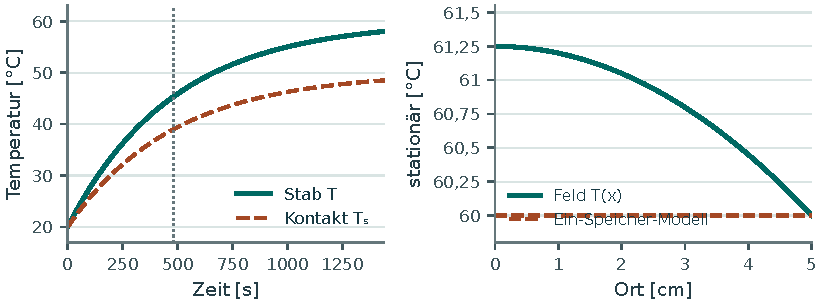
\includegraphics[width=.88\linewidth,height=49mm,keepaspectratio]{thermisch.pdf}\par}\capline{Temperatur, gespeicherte Energie und momentane Leistung bezeichnen drei verschiedene Größen.}
\seite{}{Dynamische Systeme und Steifigkeit}\anchorpage{2}{abs1-1}{1.1 · Kontinuierliche Systeme im Zustandsraum}\ey{ABSCHNITT 1.1}\ptitle{Kontinuierliche Systeme im Zustandsraum}
\hypertarget{punkt1-1-1}{}\subt{1.1.1\enspace Vektorfelder, Phasenporträts und Trajektorien}
Ein Wagen passiert zweimal dieselbe Markierung. Einmal fährt er zum Anschlag, einmal zurück. Erst der Punkt \(y=(q,v)\) unterscheidet beide Situationen. Beim Federwagen mit Masse \(m\), Federkonstante \(k\) und Dämpfung \(d\) zeigt der Pfeil an diesem Punkt in Richtung \((v,-(kq+dv)/m)\). Die Gesamtheit dieser Pfeile heißt Vektorfeld. Eine Trajektorie folgt den Pfeilen ab einem gewählten Start. Im Phasenporträt liegt die Auslenkung auf der waagerechten, die Geschwindigkeit auf der senkrechten Achse. Bei positiver Auslenkung und Geschwindigkeit null zeigt der Pfeil abwärts.
\hypertarget{punkt1-1-2}{}\subt{1.1.2\enspace Autonome Systeme und die Zeit als Zustand}
Wird der Wagen von außen mit \(F_0\cos(\omega t)\) angeregt, können am gleichen Punkt zu zwei Zeiten verschiedene Pfeile stehen. Ergänzen wir die Uhr \(s'=1,\ s(0)=t_0\), wird das erweiterte Feld \((s',q',v')=(1,v,(F_0\cos(\omega s)-kq-dv)/m)\) autonom. Die zusätzliche Koordinate trägt die Phase der Anregung.
\hypertarget{punkt1-1-3}{}\subt{1.1.3\enspace Bilanzen, Erhaltungsgrößen und Hamilton-Systeme}
Mit Impuls \(p=mv\) und Energie \(H=p^2/(2m)+kq^2/2\) gelten ohne Antrieb und Reibung \(q'=H_p,\ p'=-H_q\). Die Kettenregel ergibt \(H'=H_qH_p-H_pH_q=0\). Die geschlossenen Ellipsen im Phasenporträt sind Energieniveaus. Reibung ergänzt \(-dv\) in der Impulsbilanz und liefert \(H'=-dv^2\). Eine nach außen wandernde Rechnung kann dann bereits durch das Vorzeichen der Energiebilanz widerlegt werden.
\seite{Rechenbeispiel}{Dynamische Systeme und Steifigkeit}\anchorpage{2}{kap1}{Welche Information fehlt dem Messgerät?}\ptitle{Welche Information fehlt dem Messgerät?}


\lernziel{Sie können aus zwei Beobachtungen einen Zustand bestimmen und angeben, welche äußere Größe für eine Vorhersage noch fehlt.}
Ein Vorratsbehälter hat laut Anzeige genau 12 Liter Inhalt. In fünf Sekunden soll ein Ventil öffnen, falls dann mindestens 14 Liter bereitstehen. Können Sie das Ventil schon jetzt freigeben? Zeichnen Sie zwei mögliche Füllkurven durch denselben angezeigten Punkt.
\subt{Was wir über den Behälter annehmen}
Im betrachteten Zeitfenster läuft er weder über noch leer. Zufluss und Abfluss seien je Versuch konstant. Ein Durchflussmesser zeigt in Versuch A einen Nettozufluss von \(0{,}6\unitm{L/s}\), in Versuch B sind es \(0{,}2\unitm{L/s}\). Das Vorzeichen „plus“ bedeutet, dass Wasser im Behälter hinzukommt.
\subt{Eine Vorhersage für jeden Versuch}
In A kommen \(5\cdot0{,}6=3\unitm L\) hinzu. Der Behälter erreicht \(15\unitm L\). In B kommt nur ein Liter hinzu. Mit \(13\unitm L\) bleibt das Ventil zu. Die Zahl auf der Anzeige war in beiden Fällen richtig. Die Zukunft hing zusätzlich davon ab, was während der fünf Sekunden von außen zugeführt wurde.
\notebox{Jetzt Sie}{Die Anzeige bleibt bei \(12\unitm L\). Welcher konstante Nettozufluss reicht gerade? Schreiben Sie erst einen Bruch mit Einheiten. Die Kontrolle lautet \( (14-12)\unitm L/(5\unitm s)=0{,}4\unitm{L/s}\). Bei genau diesem Wert öffnet das Ventil.}
Beim Wagen führt dieselbe Frage zu einer anderen fehlenden Information. Selbst wenn alle künftigen Kräfte bekannt sind, genügt die aktuelle Position allein noch nicht.

\srcs{\textbf{Kernweg}\enspace\see{grund}{Zustand des Wagens}\quad\textbf{Vertiefung}\enspace\see{periodenformel}{Exakte Pendelperiode}\quad\see{ueb1}{Selbst prüfen}.}

\lektion{Wie viel Gegenwart braucht eine Vorhersage?}{grund}{Kernweg}{Dynamische Systeme}
\vorhersage{1}{Zwei Pumpen haben zu Beginn und am Ende einer Sekunde dieselben Förderraten. Liefern sie gleich viel Wasser?}{kontrolleA}
Eine Lichtschranke zählt einen Wagen bei \(q=1\unitm m\). Die Strecke ist horizontal und der Wagen rollt eine Sekunde lang kräftefrei. Zeichnen Sie zwei Pfeile durch denselben Ort. Mit \(v=+0{,}5\unitm{m/s}\) liegt der Wagen danach bei \(1{,}5\unitm m\), mit \(v=-0{,}5\unitm{m/s}\) bei \(0{,}5\unitm m\). Welche zweite Angabe fehlt der Lichtschranke?
\minifig{zustaende}{42mm}{Links laufen beide Bahnen durch denselben Messpunkt. Rechts unterscheidet die zweite Koordinate, die Geschwindigkeit, die beiden Bewegungen.}
\subt{System, Zustand, Eingang, Ausgang}
Ein \emph{System} ist der abgegrenzte Gegenstand unserer Beschreibung. Sein \emph{Zustand} fasst für die betrachtete Aufgabe alle Informationen zusammen, die bei bekanntem künftigen Eingang die weitere Entwicklung bestimmen. Der \emph{Eingang} kann von außen vorgegeben werden, etwa die Zugkraft. Der \emph{Ausgang} ist die beobachtete Größe, etwa die Lichtschrankenposition. Eine zeitliche Folge von Zuständen heißt \emph{Trajektorie}.

Für den kraftfreien Wagen genügt das Paar \((q,v)\). Auch eine einzelne Masse auf einer Feder lässt sich so beschreiben. Eine zweite bewegliche Masse könnte zusätzliche Zustände erfordern.
\notebox{Selbstkontrolle}{Ein Tank enthält 20 Liter. Kennen wir den konstanten Querschnitt und alle Zu- und Abflüsse bis in zehn Sekunden, können wir den künftigen Pegel berechnen. Bei unbekannter Ventilstellung fehlt ein Eingang.}

\lektion{Von zwei Messpunkten zur Bilanz}{ableitung}{Kernweg}{Dynamische Systeme}
Der Wagen passiert bei \(t=0\unitm s\) und \(t=2\unitm s\) die Marken \(q=1\unitm m\) und \(q=2\unitm m\). Die mittlere Geschwindigkeit im Intervall ist \( (2-1)/(2-0)=0{,}5\unitm{m/s}\). Bei veränderlicher Geschwindigkeit interessiert die Steigung der Ortskurve genau jetzt. Für einen glatten Verlauf definieren wir
\[
 v(t)=\dot q(t)=q'(t)=\lim_{h\to0}\frac{q(t+h)-q(t)}{h}.
\]
Ein Punkt bedeutet zeitliche Ableitung. Der zweite Punkt \(\ddot q=\dot v\) bedeutet Beschleunigung. Für \(q(t)=q_0+v_0t+at^2/2\) ergibt der Differenzenquotient \(v_0+at+ah/2\). Sein Grenzwert ist \(v_0+at\). Die Einheit wechselt bei jeder Zeitableitung um einen Faktor \(\mathrm{s}^{-1}\).
\subt{Rückwärts denken führt zum Integral}
In einem kurzen Intervall \(\Delta t_i\) legt der Wagen ungefähr \(v(t_i)\Delta t_i\) zurück. Addiert man diese Beiträge und lässt die größte Intervalllänge gegen null gehen, entsteht für stetiges \(v\) das bestimmte Integral
\[
 q(b)-q(a)=\int_a^b v(t)\dg t.
\]
Bei \(v(t)=2t\unitm{m/s}\) für den Zahlenwert \(t\) in Sekunden ergibt die Dreiecksfläche von 0 bis 3 Sekunden \(9\unitm m\). Differenzieren und Integrieren verbinden eine momentane Rate mit der Änderung im ganzen Zeitintervall. Das ist die Grundlage jeder Speicherbilanz.
\subt{Eine Gleichung aus Worten gewinnen}
Ein Tank erhält \(3\unitm{L/s}\) und gibt \(1\unitm{L/s}\) ab. In fünf Sekunden wächst sein Inhalt um \(10\unitm L\). In Symbolen lautet die Bilanz \(\dot V=Q_\mathrm{ein}-Q_\mathrm{aus}\). Diese Gleichung bestimmt die Änderung. Erst die zusätzliche Angabe \(V(0)=20\unitm L\) legt den Inhalt nach fünf Sekunden auf \(30\unitm L\) fest. Eine Funktion zusammen mit ihren geforderten Anfangsdaten zu bestimmen heißt, ein \emph{Anfangswertproblem} zu lösen.
\notebox{Einheitenprobe}{In einer Summe müssen alle Summanden dieselbe physikalische Dimension haben. Im Tank steht auf beiden Seiten Volumen pro Zeit. Eine Formel \(\dot V=Q_\mathrm{ein}-V\) braucht vor \(V\) einen Faktor mit der Einheit \(1/\mathrm s\).}

\lektion{Braucht diese Aufgabe einen Zeitschritt?}{methodenwahl}{Kernweg}{Dynamische Systeme}
Ein Tank enthält 20 Liter. Pro Sekunde fließen drei Liter hinein und einer hinaus. Wie viel Wasser ist nach fünf Sekunden im Tank? Bei konstanten Raten gilt bis zum Überlauf für die Zeit \(t\) in Sekunden
\[
 V(t)=(20+2t)\unitm L .
\]
Nach fünf Sekunden sind es \(30\unitm L\). Umgekehrt folgt aus \(20+2t=40\), dass die 40-Liter-Marke nach zehn Sekunden erreicht ist.
\subt{Was ändert sich bei einem geregelten Ventil?}
Nun misst ein Sensor den Zufluss. Der Abfluss hängt vom Wasserstand ab. Bei einem Grenzstand schaltet der Regler das Ventil. Für jeden Schritt berechnen wir aus den Flüssen den neuen Stand und daraus den nächsten Abfluss. Überschreitet der Stand die Schwelle, suchen wir die Schaltzeit innerhalb des Schritts. Dafür müssen wir auch festlegen, wie wir den Zufluss zwischen zwei Messwerten annähern.
\subt{Zwei Entscheidungen vor der Rechnung}
{\tblstart\begin{tabularx}{\linewidth}{@{}P{30mm}YY@{}}\toprule
\hd{Modell}&\hd{Analytisch lösen}&\hd{Numerisch lösen}\\\midrule
Ursprüngliche Gleichungen&Formel, Erhaltungssatz oder Integral für die gesuchte Größe herleiten.&Aus dem gegebenen Gesetz einzelne Werte oder eine ganze Bahn berechnen.\\
Am Arbeitspunkt linearisiertes Modell&Eine Formel beschreibt die Reaktion auf kleine Störungen.&Die linearen Gleichungen etwa mit einem aufgezeichneten, zeitlich wechselnden Eingang integrieren.\\\bottomrule\end{tabularx}\par}
Gekoppelte Gleichungen, gemessene Eingänge und viele Schaltvorgänge erschweren eine geschlossene Lösung. Auch ein lineares Wärmemodell mit tausend Temperaturen lässt sich sinnvoll numerisch auswerten.
\notebox{Entscheidung für den Versuch}{Den Füllstand bei konstanten Raten liefert die Formel. Für kleine Schwankungen um einen stationären Stand prüfen wir die Linearisierung. Für die erste Schaltzeit brauchen wir den gemessenen Zufluss, die Schaltregel und eine geforderte Zeitgenauigkeit.}
\srcs{\see{arbeitspunkt}{Arbeitspunkt und Tangente} · \see{periodentest}{Ein Fehlerziel am Pendel} · \see{c07modell}{Ereigniszeiten im ARGESIM-Versuch}.}

\lektion{Vektoren, Matrizen und ein Maß für Fehler}{vektor}{Kernweg}{Dynamische Systeme}
Ein \emph{Skalar} ist eine einzelne Zahl. Ein \emph{Vektor} fasst mehrere geordnete Zahlen zu einem Objekt zusammen. Für den Wagen schreiben wir \(x=(q,v)^\mathsf T\) als Spalte. \({}^\mathsf T\) vertauscht Zeile und Spalte. \(\mathbb R^n\) bezeichnet alle Spalten mit \(n\) reellen Einträgen. Verschiedene Einträge dürfen verschiedene Einheiten haben.
\subt{Eine Matrix als Rechenvorschrift}
Eine Matrix bildet durch Zeile-mal-Spalte einen Vektor auf einen anderen ab. Beim kraftfreien Wagen ergibt die exakte Fortrechnung über \(h\) Sekunden
\[
 \begin{pmatrix}q(t+h)\\v(t+h)\end{pmatrix}
 =\underbrace{\begin{pmatrix}1&h\\0&1\end{pmatrix}}_{A(h)}
 \begin{pmatrix}q(t)\\v(t)\end{pmatrix}.
\]
Die erste Zeile addiert den in \(h\) Sekunden zurückgelegten Weg. Die zweite übernimmt die Geschwindigkeit. Zwei Schritte \(h,k\) ergeben durch Matrixmultiplikation \(A(k)A(h)=A(h+k)\). Die Einheitsmatrix \(I=A(0)\) lässt jeden Vektor unverändert.
\subt{Lösbar und eindeutig}
Eine quadratische Matrix ist \emph{invertierbar}, wenn jede rechte Seite \(b\) in \(Ax=b\) genau eine Lösung besitzt. Bei zwei Zeilen und zwei Spalten entscheidet die Determinante \(ad-bc\) für \(A=\left(\begin{smallmatrix}a&b\\c&d\end{smallmatrix}\right)\). Sie muss ungleich null sein. Der \emph{Rang} zählt linear unabhängige Spalten, äquivalent die unabhängigen Zeilen. Zwei gleiche Messzeilen liefern nur eine unabhängige Information.
\subt{Wie groß ist ein Vektor?}
Eine Norm ordnet einem Vektor eine nichtnegative Länge zu. Die Maximumnorm ist \(\|z\|_\infty=\max_i |z_i|\), die euklidische Norm \(\|z\|_2=\sqrt{\sum_i z_i^2}\). Vor einem Zahlenvergleich zwischen Ort und Geschwindigkeit teilen wir jeden Fehler durch seine zulässige Abweichung. Bei Fehlern \(2\unitm{mm}\), \(0{,}03\unitm{m/s}\) und Grenzen \(5\unitm{mm}\), \(0{,}02\unitm{m/s}\) entsteht \(z=(0{,}4,1{,}5)^\mathsf T\). Die Maximumnorm \(1{,}5\) zeigt sofort, welche Komponente durchfällt.
\srcs{Mit demselben Gedanken bewertet das Praktikum mehrere Ereigniszeiten und Endwerte auf S.\,\pagelink{vergleich}.}

\lektion{Wie Mathematik eine Näherung beschreibt}{mathewerk}{Vertiefung}{Dynamische Systeme}
Für eine kleine Änderung \(h\) liefert die Tangente \(f(x+h)\approx f(x)+hf'(x)\). Die \emph{Taylorformel} gibt bei zweimal stetig differenzierbarem \(f\) den Rest als \(h^2 f''(\xi)/2\) an, mit \(\xi\) zwischen \(x\) und \(x+h\). Die Schreibweise \(O(h^p)\) bedeutet, dass der Betrag für hinreichend kleine \(|h|\) höchstens \(C|h|^p\) beträgt, mit einer von \(h\) unabhängigen Konstanten \(C\).
\subt{Exponent, Logarithmus und eine Zeitkonstante}
Die Exponentialfunktion \(e^z=\sum_{k=0}^\infty z^k/k!\) ist ihre eigene Ableitung. Deshalb löst \(x(t)=x_0e^{-t/\tau}\) die Gleichung \(\dot x=-x/\tau\) für \(\tau>0\). Nach einer Zeitkonstante bleibt der Anteil \(1/e\). Der natürliche Logarithmus \(\ln\) ist die Umkehrfunktion von \(e^z\) für positive reelle Argumente. Die Halbwertszeit folgt aus \(e^{-t/\tau}=1/2\), also \(t=\tau\ln 2\).
\subt{Eine Änderung in mehreren Richtungen}
Hängt \(f\) von \(x\) und \(z\) ab, variiert die partielle Ableitung \(f_x=\partial f/\partial x\) nur \(x\) bei festem \(z\). Für \(f(x,z)=xz^2\) sind \(f_x=z^2\) und \(f_z=2xz\). Entlang einer Bahn gilt die Kettenregel
\[
 \frac{\dd}{\dd t}f(x(t),z(t))=f_x\dot x+f_z\dot z .
\]
Hat die Funktion mehrere Ausgaben \(f_i\), sammelt die \emph{Jacobi-Matrix} die partiellen Ableitungen in \(J_{ij}=\partial f_i/\partial x_j\). Sie ist die lokale lineare Abbildung \(f(x+\delta x)\approx f(x)+J(x)\delta x\). Hat \(f\) zusätzlich eine ausdrückliche Zeitabhängigkeit, kommt in der Kettenregel \(f_t\) hinzu.
\subt{Wie löst man eine Gleichung, die sich nicht umstellen lässt?}
Ein \emph{Residuum} \(r(z)\) misst die Verletzung einer Gleichung. Gesucht ist eine Nullstelle. Newton löst \(r'(z_k)\Delta z=-r(z_k)\) und setzt \(z_{k+1}=z_k+\Delta z\). Für \(r=z^2-2,\ z_0=1{,}5\) folgt \(z_1=1{,}41667\). Das Verfahren braucht lokal eine brauchbare Steigung. Bei stetigem \(r\) und entgegengesetzten Vorzeichen an den Enden kann Intervallhalbierung dagegen eine Nullstelle einklammern. Ein bloßer Berührpunkt hat nicht zwingend einen Vorzeichenwechsel.

\seite{Rechenbeispiel}{Dynamische Systeme und Steifigkeit}\anchorpage{2}{kap3}{Was verraten zwei Heizversuche?}\ptitle{Was verraten zwei Heizversuche?}


\lernziel{Sie können eine Systemgrenze ziehen, gespeicherte Energie und Leistung unterscheiden und aus zwei Versuchen erkennen, welche Modellparameter messbar sind.}
Ein Heizer führt einem Metallstück \(10\unitm W\) zu. Eine Minute später ist es wärmer. Reicht diese Beobachtung, um vorherzusagen, wie heiß es im Dauerbetrieb wird? Zeichnen Sie einen Rahmen um das Metall und geben Sie jedem Energiestrom einen Pfeil.
\subt{Erst die Bilanz, dann das Bauteilgesetz}
Wir nehmen eine überall gleiche Metalltemperatur an. Seine Wärmekapazität \(C=120\unitm{J/K}\) sagt, wie viel Energie einen Temperaturanstieg um ein Kelvin bewirkt. Am Start haben Metall und Umgebung dieselbe Temperatur. Im ersten Augenblick fließt daher noch keine Wärme an die Umgebung. Die gesamte Leistung erhöht die gespeicherte Energie. Die Anfangssteigung ist \(10/120=0{,}0833\unitm{K/s}\).
\subt{Ein zweiter Versuch beantwortet eine andere Frage}
Lange nach dem Einschalten beträgt der Überschuss zur Umgebung konstant \(40\unitm K\). Jetzt muss der Abfluss die ganzen \(10\unitm W\) übernehmen. Im linearen Kontaktgesetz \(\theta=Rq\) ergibt das einen Wärmewiderstand \(R=40/10=4\unitm{K/W}\). Die Anfangssteigung lieferte \(C\), der stationäre Versuch liefert \(R\).
\notebox{Jetzt Sie}{Eine zweite Halterung halbiert \(R\) bei gleichem \(C\) und gleicher Heizleistung. Skizzieren Sie beide Aufheizkurven mit gemeinsamen Sekunden- und Kelvinachsen. Beide starten mit derselben Steigung. Die neue Kurve läuft auf \(20\unitm K\) Überschuss zu.}
Das Kapitel verwendet denselben Heizer für drei Fragen. Wie warm wird das ganze Stück? Welche Temperatur hat der Kontakt? Und wo liegt im Innern der heißeste Punkt? Jede Messfrage verlangt andere Zustandsgrößen.

\srcs{\textbf{Kernweg}\enspace\see{speicher}{Bilanz und Temperatur}\quad\textbf{Vertiefung}\enspace\see{moden}{Beobachtbarkeit}\quad\see{ueb3}{Selbst prüfen}.}

\lektion{Ein Stab, ein Heizer und zwei Kontakte}{modell}{Kernweg}{Modell und System}
\vorhersage{3}{Ein Heizer liefert konstante Leistung. Welchen Einfluss hat die doppelte Wärmekapazität auf Endtemperatur und Aufheizzeit?}{kontrolleA}
Eine Halterung führt Wärme von einem beheizten Metallstab ab. Gesucht sind die Aufwärmzeit, die höchste Dauertemperatur und die Temperatur im Kontakt. Der Heizer liefert \(10\unitm W\), die Umgebung bleibt bei \(20\,^\circ\mathrm C\), Mantel und linke Stirnfläche sind isoliert. Verfolgen Sie den Weg der Energie erst in der Skizze.
\fig{stab}{.90}{Ein positiver Wärmestrom \(q=\dot Q\) verlässt den Stab nach rechts. Zwischen den Kontaktwiderständen liegt die Temperatur \(T_s\).}
\subt{Welche Daten gehören zur Bilanz?}
{\tblstart\begin{tabularx}{\linewidth}{@{}P{47mm}rY@{}}\toprule
\hd{Größe} & \hd{Wert} & \hd{Bedeutung}\\\midrule
Länge \(L\), Querschnitt \(A\)& \(0{,}05\unitm m,\;10^{-3}\unitm{m^2}\)& konstanter Querschnitt\\
Volumetrische Wärmekapazität \(\rho c\)& \(2{,}4\cdot10^6\)& \(\mathrm{J/(m^3 K)}\)\\
Wärmeleitfähigkeit \(k\)& \(200\unitm{W/(m\,K)}\)& homogener Werkstoff\\
Widerstände \(R_1,R_2\)& \(1,\;3\unitm{K/W}\)& in Reihe zum Reservoir\\\bottomrule
\end{tabularx}\par}
Die Leistung \(P\) sei gleichmäßig im Volumen verteilt. Der Stab startet bei \(20\,^\circ\mathrm C\). Stoffwerte und Querschnitt bleiben konstant, beide Kontaktlagen speichern vernachlässigbar wenig Wärme. Eine sich erwärmende Umgebung wäre ein weiterer Speicher.
\subt{Erster Überschlag vor der Integration}
Der Stab speichert \(C=\rho cAL=120\unitm{J/K}\). Gleich nach dem Einschalten fließt am kalten Kontakt noch keine Leistung ab. Damit steigt die mittlere Temperatur anfangs um \(P/C=1/12\unitm{K/s}\). Im Dauerbetrieb muss dieselbe Leistung, die eintritt, über die Halterung austreten. Diese zwei Werte prüfen später jede Simulation.
\srcs{Annahmen, Geometrie und Zahlenwerte sind Lehrbeispieldaten.}

\lektion{Aus der Energiebilanz folgt eine ODE}{speicher}{Kernweg}{Modell und System}
Wir ersetzen die Temperaturverteilung vorläufig durch eine einzige Temperatur \(T(t)\). Mit \(\theta=T-T_a\) in Kelvin und \(R=R_1+R_2=4\unitm{K/W}\) folgt aus dem Energieinhalt \(C\theta\) und dem Ausfluss \(q=\theta/R\)
\[
 C\dot\theta=P-\frac{\theta}{R},\qquad \theta(0)=0.
\]
Links steht die Änderungsrate \(\dot E=C\dot\theta\) der gespeicherten Energie \(E=C\theta\). Alle Terme der Bilanz haben die Einheit Watt. Nach Wahl von \(P(t)\) und \(\theta(0)\) ist die Ableitung bestimmt. Das ist ein Anfangswertproblem für eine gewöhnliche Differentialgleichung (ODE).
\subt{Die Rechnung für einen Leistungssprung}
Im Gleichgewicht gilt \(\theta_\infty=RP=40\unitm K\). Für \(w=\theta-\theta_\infty\) bleibt \(\dot w=-w/(RC)\). Trennung der Variablen liefert
\[
 \theta(t)=40(1-e^{-t/480})\unitm K,\qquad \tau=RC=480\unitm s
\]
mit \(t\) in Sekunden. Nach \(60\unitm s\) liegen \(24{,}700124\,^\circ\mathrm C\) vor. Der Stab hat relativ zum Start \(C\theta=564{,}015\unitm J\) gespeichert. In diesem Moment steigt seine Energie mit \(10\unitm W-\theta/R=8{,}82497\unitm W\). Nach \(\tau\) sind \(1-e^{-1}=63{,}2\,\%\) des Temperaturanstiegs erreicht. Der Kontakt folgt aus \(T_s=T_a+R_2q\). Im stationären Zustand ergibt das \(50\,^\circ\mathrm C\).
\fig{thermisch}{.96}{Links folgt der Kontakt dem Stab mit kleinerem Temperaturhub. Rechts zeigt das räumliche Modell unter denselben Randbedingungen, wo ein Ein-Speicher-Modell die Höchsttemperatur unterschätzt.}
\notebox{Reicht ein Speicher?}{Der innere Leitwiderstand hat die Skala \(L/(kA)=0{,}25\unitm{K/W}\). Das Verhältnis zur äußeren Reihenschaltung beträgt \(0{,}0625\). Der räumliche Temperaturabfall kann für die Aufwärmzeit klein und für einen Grenzwert von nur \(0{,}5\unitm K\) dennoch entscheidend sein.}
\srcs{Die stationäre Feldlösung wird auf S.\,\pagelink{pde} aus denselben Stoffdaten hergeleitet.}

\lektion{ODE, DAE und PDE am selben Gegenstand}{klassen}{Kernweg}{Modell und System}
Nehmen Sie denselben Stab. Zuerst interessiert nur eine gut durchmischte Temperatur. Dann wollen wir den Wärmestrom am Kontakt direkt ausgeben. Zuletzt fragen wir nach der heißesten Stelle im Stab. Die Physik bleibt wiedererkennbar, aber jede Aufgabenstellung braucht andere Unbekannte.
{\tblstart\begin{tabularx}{\linewidth}{@{}P{17mm}YY@{}}\toprule
\hd{Form}&\hd{Unbekannte und Gleichung}&\hd{Physikalische Aussage}\\\midrule
ODE&\(\theta(t)\), \(\ C\dot\theta=P-\theta/R\)&Ein Wärmespeicher. Der Wärmestrom ist bereits eliminiert.\\
DAE&\(\theta(t),\,\theta_s(t),\,q(t)\), \(\ C\dot\theta=P-q\) mit zwei Kontaktgesetzen&Ein Wärmespeicher und zwei augenblickliche Beziehungen.\\
PDE&\(T(x,t)\), \(\ \rho c A\,T_t=kA\,T_{xx}+P/L\)&Jedes Stabstück speichert Wärme. Ort, Randwerte und Anfangsprofil werden gebraucht.\\\bottomrule
\end{tabularx}\par}
\subt{Zwei verschiedene Entscheidungen}
\textbf{Algebraische Elimination.} Aus \(\theta-\theta_s=R_1q\) und \(\theta_s=R_2q\) folgt exakt \(q=\theta/(R_1+R_2)\). Damit sind ODE und DAE für die Stabtemperatur bei konsistenten Daten gleichwertig. Eine eigene Wärmekapazität des Kontakts würde das Modell verändern.

\textbf{Räumliche Mittelung.} Die exakte Integralbilanz lautet \(C\dot{\bar T}=P-q(L,t)\), wobei \(\bar T=L^{-1}\int_0^L T(x,t)\dg x\). Der Randstrom hängt von \(T(L,t)\) ab. Erst die Annahme \(T(L,t)\approx\bar T(t)\) schließt die Gleichung für einen einzigen Speicher. Hier entsteht ein Modellfehler.
\subt{Wie passen PDE und DAE zusammen?}
Die PDE kann am Rand mit einer algebraischen Kontaktgleichung gekoppelt sein. Diskretisiert man den Ort, erhält man Differentialgleichungen für Zelltemperaturen. Ein beibehaltener masseloser Kontakt fügt algebraische Gleichungen hinzu. Nach Elimination dieses Kontakts bleibt in diesem Beispiel eine ODE für die Zelltemperaturen.
\task{1}{Für einen thermisch trägen Kontakt mit Wärmekapazität \(C_s>0\) treten links \(q_1\) ein und rechts \(q_2\) aus. Stellen Sie das Zweitemperaturmodell auf. Welche Gleichung entsteht im Grenzmodell \(C_s=0\)?}

\lektion{Was ein Zustand über die Zukunft verrät}{system}{Kernweg}{Modell und System}
Was müssen Sie beim Speichern einer laufenden Simulation sichern, damit ein Neustart dieselbe Zukunft erzeugt? Beim ideal durchmischten Stab genügt die Temperatur, wenn die zukünftige Heizleistung bekannt ist. Bei einer fallenden Kugel gehört auch die Geschwindigkeit dazu. Von gleicher Höhe kann eine Kugel gerade steigen und die andere fallen.
\subt{Eingang, Zustand und Ausgang}
Im Modell \(\dot x=f(x,u,t),\ y=h(x,u,t)\) bezeichnet \(u\) die von außen vorgegebene Anregung und \(y\) die Messgröße. Für ein lineares, zeitinvariantes System (LTI) mit konstanten Matrizen gilt
\[
 \dot x=A_sx+B_su,\qquad y=C_s^{\rm out}x+D_s u .
\]
Die Indizes unterscheiden Systemmatrizen von Fläche und Wärmekapazität. Beim Stab mit \(u=P,\ x=\theta,\ y=\theta\) sind \(A_s=-1/(RC),\ B_s=1/C,\ C_s^{\rm out}=1,\ D_s=0\).
\subt{Zeitantwort und Frequenzantwort aus derselben Gleichung}
Variation der Konstanten ergibt
\[
 x(t)=e^{A_st}x(0)+\int_0^t e^{A_s(t-s)} B_su(s)\dg s .
\]
Zur Kontrolle differenziert man die rechte Seite. Die obere Integrationsgrenze liefert \(B_su(t)\), die übrigen Terme ergeben \(A_sx(t)\). Bei Anfangswert null folgt durch Laplace-Transformation die Übertragungsfunktion
\[
 G(s)=C_s^{\rm out}(sI-A_s)^{-1}B_s+D_s=\frac{R}{1+sRC}
 \quad\text{für den Stab.}
\]
Im stationären Sinusbetrieb ist der Verstärkungsbetrag \(R/\sqrt{1+(\omega\tau)^2}\), die Phase \(-\arctan(\omega\tau)\). Bei \(\omega=1/\tau\) bedeuten \(1\unitm W\) Eingangsamplitude \(4/\sqrt 2=2{,}83\unitm K\) Ausgangsamplitude und \(45^\circ\) Nacheilen. Der Pol \(-1/\tau\) bestimmt also Aufwärmzeit und Grenzfrequenz zugleich.
\srcs{\refbk{sy}{Åström und Murray, Feedback Systems} · Zustand, lineare Dynamik und Eingangs-/Ausgangsbeschreibung.}

\lektion{Vom Rechnen mit Matrizen zur Systemtheorie}{linearsprache}{Kernweg}{Modell und System}
Eine Abbildung \(A\) heißt \emph{linear}, wenn \(A(\alpha x+\beta z)=\alpha A x+\beta A z\). Damit lassen sich Antworten auf einzelne Anregungen addieren. \emph{Zeitinvariant} bedeutet, dass eine Verschiebung des gesamten Versuchs in der Zeit dasselbe Verhalten mitverschiebt. Ein System mit konstanten Matrizen ist ein wichtiges Beispiel.
\subt{Warum Eigenwerte in einer Zeitentwicklung auftauchen}
Erfüllt ein Vektor \(w\ne0\) die Gleichung \(Aw=\lambda w\), heißt \(w\) Eigenvektor und \(\lambda\) Eigenwert. Für \(\dot x=Ax\) löst dann \(x=e^{\lambda t}w\) die Differentialgleichung, wie Ableiten zeigt. Ein solcher Bewegungsanteil heißt \emph{Mode}. Das Matrixexponential \(e^{At}=I+At+(At)^2/2!+\cdots\) fasst die Fortrechnung für alle Anfangsvektoren zusammen.

Komplexe Zahlen \(s=\sigma+\mathrm i\omega\) verwenden \(\mathrm i^2=-1\). Wegen \(e^{st}=e^{\sigma t}(\cos\omega t+\mathrm i\sin\omega t)\) beschreibt \(\sigma\) Wachstum oder Abklingen und \(\omega\) eine Kreisfrequenz in Radiant pro Sekunde. Ein Radiant ist der Winkel, dessen Bogenlänge auf einem Kreis gleich dem Radius ist. Eine volle Umdrehung entspricht \(2\pi\) Radiant. Die reale Messgröße kann einfach der Realteil sein.
\subt{Ein Werkzeug für Eingangs- und Ausgangsgrößen}
Die Laplace-Transformierte eines Signals \(w(t)\) ist \(W(s)=\int_0^\infty e^{-st}w(t)\dg t\), wo das Integral konvergiert. Partielle Integration liefert \(\mathcal L\{\dot w\}=sW(s)-w(0)\). Eine Differentialgleichung wird so zur algebraischen Beziehung in \(s\).

Beim Stab ergibt \(C\dot\theta+\theta/R=P\) bei kaltem Start \((Cs+1/R)\Theta(s)=P(s)\). Der Quotient \(G(s)=\Theta(s)/P(s)\) heißt \emph{Übertragungsfunktion}. Ein \emph{Pol} ist hier eine Nullstelle des Nenners, an der der Quotient unbeschränkt wird. Die Position \(-1/(RC)\) ist dieselbe Abklingrate, die die Zeitlösung enthält. Für stabilen eingeschwungenen Sinusbetrieb setzt man \(s=\mathrm i\omega\).
\srcs{\refbk{sy}{Åström und Murray, Zustandsraum und Frequenzantwort} · \see{arbeitspunkt}{Wie aus einem nichtlinearen System ein lokales lineares Modell wird}.}

\lektion{Was bedeutet Linearisieren im Arbeitspunkt?}{arbeitspunkt}{Kernweg}{Dynamische Systeme}
Ein Pendel hängt senkrecht und ruht. Eine kleine Auslenkung erzeugt eine rücktreibende Beschleunigung. Für einen Entwurf nahe dieser Lage interessiert zunächst, wie sich die Beschleunigung bei einer kleinen Störung ändert. Dafür genügt häufig die Tangente an das Bewegungsgesetz.
\subt{Vom Arbeitspunkt zur Gleichung für kleine Abweichungen}
Bei einem zeitunabhängigen Gesetz \(\dot x=f(x,u)\) ist ein \emph{stationärer Arbeitspunkt} ein Paar aus Zustand \(x_*\) und konstantem Eingang \(u_*\) mit \(f(x_*,u_*)=0\). Für \(\delta x=x-x_*,\ \delta u=u-u_*\) liefert die Taylorformel
\[
 \delta\dot x=A\,\delta x+B\,\delta u+r,\qquad
 A=\left.\frac{\partial f}{\partial x}\right|_*,\quad
 B=\left.\frac{\partial f}{\partial u}\right|_* .
\]
Die Matrizen geben an, wie sich jede Steigung mit Zustand und Eingang ändert. Bei zweimal stetig differenzierbarem \(f\) ist der Rest nach geeigneter Skalierung lokal von der Größenordnung \(\|(\delta x,\delta u)\|^2\). Das lineare Modell setzt \(r=0\). Es eignet sich beispielsweise für die Frequenz kleiner Schwingungen oder die Auslegung eines Reglers nahe seinem Sollwert.
\subt{Am Pendel lässt sich die Tangente ausrechnen}
Seien \(L\) die Länge, \(g\) die Fallbeschleunigung und \(u\) eine von außen aufgeprägte Winkelbeschleunigung. Mit \(\theta\) als Winkel zur unteren Senkrechten, in Radiant, und \(\omega=\dot\theta\) gilt ohne Reibung
\[
 \dot\theta=\omega,\qquad \dot\omega=-(g/L)\sin\theta+u .
\]
Am Arbeitspunkt \((\theta_*,\omega_*,u_*)=(0,0,0)\) ist die Steigung des Sinus gleich eins. Bei \(u=0\), Startwinkel \(\theta_0\) und Startgeschwindigkeit null führt \(\sin\theta\approx\theta\) zu
\[
 \theta_{\rm lin}(t)=\theta_0\cos\!\big(\sqrt{g/L}\,t\big),\qquad
 T_0=2\pi\sqrt{L/g}.
\]
Einsetzen bestätigt diese Lösung des linearen Modells. Dessen Periodendauer \(T_0\) ist für jede von null verschiedene Amplitude gleich. Beim ursprünglichen Pendel hängt die Dauer von der Amplitude ab. Wie groß der Unterschied ist, können wir ohne Messgerät herleiten.
\srcs{\href{https://underactuated.mit.edu/acrobot.html}{Tedrake, Linearisierung an einem Fixpunkt} · \href{https://openstax.org/books/university-physics-volume-1/pages/15-4-pendulums}{OpenStax, Pendel und Kleinwinkelnäherung}.}

\lektion{Welche Mode sieht der Sensor?}{moden}{Vertiefung}{Modell und System}
Zwei gleiche Metallblöcke haben je \(C_b=60\unitm{J/K}\). Jeder gibt über \(G_e=0{,}125\unitm{W/K}\) Wärme an dieselbe Umgebung ab. Zwischen beiden fließen \(G_c(\theta_1-\theta_2)\) Watt mit \(G_c=2\unitm{W/K}\). Ein Heizer wirkt nur am ersten Block. Die Kontaktleistung tritt mit entgegengesetztem Vorzeichen in die beiden Bilanzen ein.
\[
 \dot x=\begin{bmatrix}-(a+b)&b\\ b&-(a+b)\end{bmatrix}x+
 \begin{bmatrix}1/C_b\\0\end{bmatrix}P,\qquad
 a=G_e/C_b,\quad b=G_c/C_b .
\]
Addiert man die Bilanzen, verschwindet der innere Wärmestrom. Subtrahiert man sie, verdoppelt sich sein Einfluss. Die Eigenvektoren \((1,1)^\mathsf T\) und \((1,-1)^\mathsf T\) beschreiben gemeinsame Erwärmung und Temperaturdifferenz. Ihre Zeitkonstanten betragen \(1/a=480\unitm s\) und \(1/(a+2b)=14{,}55\unitm s\).
\subt{Anregbar und beobachtbar sind verschiedene Eigenschaften}
Für zwei LTI-Zustände bedeutet voller Rang von \([B_s,A_sB_s]\), dass ein geeigneter Eingang jeden Zustand in endlicher Zeit erreichen kann. Hier ist die Determinante \(b/C_b^2\ne0\). Der links angebrachte Heizer kann beide Moden anregen.

Ein Mittelwertsensor hat die Messzeile \(H=(1/2,1/2)\). Aus \(HA_s=-aH\) folgt, dass die Zeilen von \(\left[\begin{smallmatrix}H\\HA_s\end{smallmatrix}\right]\) linear abhängig sind. Temperaturdifferenzen sind bei bekanntem Eingang aus diesem Ausgang allein unbeobachtbar. Ein Sensor am ersten Block hat dagegen \(H=(1,0)\). Die Determinante derselben Beobachtbarkeitsmatrix ist dann \(b\ne0\).
\minifig{moden}{27mm}{Eine reine Temperaturdifferenz klingt ab, während der Mittelwertsensor ständig null meldet. Die getrennten Fühler machen die schnelle Mode sichtbar.}
\notebox{Konsequenz für den Vergleich}{Ein Solver kann den Mittelwert ausgezeichnet treffen und die schnelle Differenzmode schlecht darstellen. Im Experiment trennen ein Mittelwert und eine lokale Temperatur beide Aussagen.}
\task{2}{Anfangs gelten \(\theta_1=10\unitm K,\ \theta_2=-10\unitm K,\ P=0\). Welche Kurve sieht der Mittelwertsensor? Welche Temperatur misst der linke Sensor nach \(14{,}55\unitm s\)?}

\lektion{Physikalische Stabilität begründen}{lyapunov}{Vertiefung}{Modell und System}
Ein Federpendel mit Masse \(m>0\), Federsteifigkeit \(k_f>0\) und viskoser Dämpfung \(d\ge0\) bewegt sich horizontal. Die Auslenkung \(q\) startet bei \(q_0\), die Geschwindigkeit \(v\) bei \(v_0\). Newtons Gesetz addiert Federkraft \(-k_fq\), Reibung \(-dv\) und äußere Kraft \(F\). Die Bewegungsgleichungen lauten
\[
 \dot q=v,\qquad m\dot v=F-dv-k_fq .
\]
Ohne äußere Kraft ist \((0,0)\) eine Ruhelage. Stabil im Sinne von Lyapunov bedeutet, dass hinreichend nahe Starts für alle künftigen Zeiten nahe bleiben. Asymptotische Stabilität verlangt zusätzlich Rückkehr zur Ruhelage.
\subt{Satz · Die Energiebilanz bestimmt das Langzeitverhalten}
Für \(F=0\) bleibt die Ruhelage bei \(d=0\) stabil. Für \(d>0\) ist sie asymptotisch stabil.
\proofpart{Die mechanische Energie \(V=(mv^2+k_fq^2)/2\) ist positiv definit. Ableiten entlang einer Lösung ergibt \(\dot V=mv\dot v+k_fq\dot q=Fv-dv^2\). Bei \(F=0\) und \(d=0\) sind die Energieniveaus geschlossene Ellipsen. Kleine Anfangsenergie hält beide Zustände klein. Für \(d>0\) besitzt das charakteristische Polynom \(ms^2+ds+k_f\) zwei Wurzeln mit negativem Realteil. Alle Lösungen des homogenen linearen Systems klingen daher ab, auch im Fall einer Doppelwurzel.}
\subt{Aus dem Beweis wird ein Test}
Der dämpfungsfreie Oszillator darf seine Energie über lange Zeit behalten und trotzdem eine falsche Phase besitzen. Bei \(d>0\) ist Energieverlust physikalisch. Ein numerischer Versuch prüft dann zusätzlich, ob der Verlust der berechneten Reibungsarbeit entspricht. Bei äußerer Kraft gehört die zugeführte Arbeit \(\int Fv\dg t\) ebenfalls in die Bilanz.
\notebox{Linearisierung}{Nahe einem Gleichgewicht ersetzt der Jacobi-Operator \(A_s=\partial f/\partial x\) die nichtlineare Dynamik in erster Näherung. Strikt negative Realteile aller Eigenwerte sichern bei stetig differenzierbarem \(f\) lokale asymptotische Stabilität. Eigenwerte auf der imaginären Achse verlangen weitere Analyse.}
\srcs{\refbk{sy}{Feedback Systems} · Die Phasen- und Energierechnung für den dämpfungsfreien Fall steht auf S.\,\pagelink{verlet}.}

\lektion{Wann genügt die Kleinwinkelformel?}{periodentest}{Kernweg}{Dynamische Systeme}
Ein Pendel von \(L=1\unitm m\) schwingt bei \(g=9{,}81\unitm{m/s^2}\). Die Periodendauer soll höchstens um \(1\,\%\) von der des nichtlinearen Modells abweichen. Wir messen den Fehler relativ zu dessen exakter Periode \(T\), also \(e=(T-T_0)/T\).
{\tblstart\begin{tabularx}{\linewidth}{@{}Yrrrr@{}}\toprule
\hd{Startwinkel}&\hd{Linear \(T_0\) [s]}&\hd{Exakt \(T\) [s]}&\hd{Numerisch [s]}&\hd{Fehler \(e\)}\\\midrule
\(5^\circ\)&2,006067&2,007022&2,007022&0,048\,\%\\
\(15^\circ\)&2,006067&2,014694&2,014694&0,428\,\%\\
\(30^\circ\)&2,006067&2,040990&2,040990&1,711\,\%\\
\(60^\circ\)&2,006067&2,152875&2,152875&6,819\,\%\\\bottomrule\end{tabularx}\par}
Da \(T\) streng wächst, gibt es genau einen Grenzwinkel für \(e=0{,}01\). Er liegt bei rund \(22{,}93^\circ\). Diese Aussage gilt für die \emph{Periode} unter den genannten Annahmen. Für den Winkelfehler nach zehn Sekunden braucht man ein eigenes Kriterium.
\minifig{periodendrift}{44mm}{Bei \(60^\circ\) Startauslenkung bleiben die maximalen Winkel gleich groß. Die dritte Rückkehr zur Startlage erfolgt im linearen Modell rund \(0{,}44\unitm s\) früher.}
\subt{Wie die numerische Spalte geprüft wurde}
DOP853 passt seine Schrittweite an den geschätzten Fehler an. Wir integrieren die Sinusgleichung bis zum ersten fallenden Nulldurchgang und vervierfachen die Zeit. Beim Verfeinern von \(h_{\max}=0{,}2\) auf \(0{,}1\unitm s\) und der relativen Toleranz von \(10^{-6}\) auf \(10^{-10}\) sinkt die größte gemessene Abweichung zur Integralformel von \(1{,}1\cdot10^{-8}\) auf unter \(1{,}3\cdot10^{-11}\unitm s\). Die absolute Toleranz beträgt jeweils ein Hundertstel der relativen. Ein kleinerer Schritt in der linearen Gleichung nähert sich dagegen deren eigener Periode \(T_0\). Der Modellfehler \(T-T_0\) bleibt.
\notebox{Selbstkontrolle}{Bei \(30^\circ\) und \(2\,\%\) erlaubtem Periodenfehler genügt die Linearisierung. Wäre auch der Zeitpunkt der zehnten Rückkehr auf \(0{,}2\unitm s\) genau? Aus ungerundeten Werten folgt \(10(T-T_0)=0{,}349\unitm s\). Für dieses zweite Ziel reicht die Näherung nicht aus.}
\srcs{Nachrechnung mit \texttt{python labor.py periode}. Der \see{c07modell}{Vergleich mit dem Anschlagstift} untersucht dieselbe Frage für Kontaktzeiten.}

\lektion{Die exakte Periode des nichtlinearen Pendels}{periodenformel}{Vertiefung}{Dynamische Systeme}
Ein starrer, masseloser Stab der Länge \(L\) trägt eine Punktmasse. Die Lagerung ist reibungsfrei, die Schwerkraft konstant. Wir lassen die Masse bei \(0<\theta_0<\pi\) aus der Ruhe los. Wie lange braucht sie, um erstmals in diese Lage und Bewegungsphase zurückzukehren? Gesucht ist eine Zahl \(T\). Dafür reicht eine Energiebilanz.
\subt{1. Einmal integrieren}
Multiplizieren wir \(\ddot\theta+(g/L)\sin\theta=0\) mit \(L^2\dot\theta\), erhalten wir die Zeitableitung der mechanischen Energie pro Masse. Sie verschwindet. Die Anfangsdaten bestimmen ihre Konstante:
\[
 \tfrac12 L^2\dot\theta^2+gL(1-\cos\theta)=gL(1-\cos\theta_0).
\]
Auf dem ersten Weg zur Senkrechten fällt \(\theta\). Dort wählen wir die negative Wurzel, \(\dot\theta=-\sqrt{(2g/L)(\cos\theta-\cos\theta_0)}\). Spiegelung an der Senkrechten und Zeitumkehr ergeben vier gleich lange Viertelschwingungen.
\subt{2. Den Weg in eine Zeit umrechnen}
Aus \(\dg t=\dg\theta/\dot\theta\) folgt die Periodendauer. Setzen wir im Integral \(\sin(\theta/2)=\sin(\theta_0/2)\sin\psi\), so werden aus den Grenzen \(0,\theta_0\) die festen Grenzen \(0,\pi/2\). Mit \(\cos\theta=1-2\sin^2(\theta/2)\) ergibt sich
\[
 \frac{T}{4}=\sqrt{\frac{L}{2g}}\int_0^{\theta_0}
 \frac{\dg\theta}{\sqrt{\cos\theta-\cos\theta_0}}
 =\sqrt{\frac{L}{g}}\int_0^{\pi/2}\frac{\dg\psi}{\sqrt{1-\mu\sin^2\psi}},
 \qquad \mu=\sin^2(\theta_0/2).
\]
Das letzte Integral heißt vollständiges elliptisches Integral erster Art, hier mit dem \emph{Parameter} \(\mu\) als Argument \(K(\mu)\). Damit ist \(T=4\sqrt{L/g}\,K(\mu)\) eine exakte Formel für das gewählte Modell. Den Dezimalwert kann ein Rechner durch numerische Auswertung des Integrals liefern.
\subt{3. Eine Vorhersage prüfen}
Bei wachsendem \(\theta_0\) wächst \(\mu\). Der Integrand wächst für \(0<\psi<\pi/2\) streng. Folglich wächst die Periodendauer. Für \(\theta_0\to0\) geht der Integrand gleichmäßig gegen eins, das Integral gegen \(\pi/2\) und \(T\) gegen \(T_0\). Die Kleinwinkelformel unterschätzt also jede Periode mit endlicher, positiver Amplitude in diesem Bereich.
\srcs{\href{https://dlmf.nist.gov/22.19}{NIST DLMF §22.19(i), Darstellung mit Modul \(k=\sqrt\mu\)} · \href{https://docs.scipy.org/doc/scipy/reference/generated/scipy.special.ellipk.html}{SciPy, elliptisches Integral mit Parameter \(\mu\)}.}

\clearpage\anchorpage{1}{dreiwege}{Formel, Linearisierung und Zeitschritte am selben Tank}\ptitle{Drei Rechnungen am selben Tank}
Ein Tank soll nach einer Minute mindestens halb so hoch wie sein stationärer Pegel gefüllt sein. Wir messen den Pegel \(H\) als Anteil dieses stationären Werts und die Zeit \(s\) in Einheiten von einer Minute. Ein konstanter Zulauf und ein quadratisches Ablaufgesetz liefern das Lehrmodell \(H'=(1-H^2)/2\). Bei \(H=1\) sind Zu- und Abfluss gleich. Das ist der \emph{Arbeitspunkt}.
\subt{Eine Formel, eine Tangente und zwei Schritte}
Starten wir leer, also mit \(H(0)=0\). Eine exakte Lösung ist \(H(s)=(e^s-1)/(e^s+1)\). Sie beginnt bei null und erfüllt das Gesetz, wie sich durch Ableiten prüfen lässt. Ihr Wert nach einer Minute beträgt \(0{,}46212\).

Für die \emph{Linearisierung} schreiben wir \(H=1+x\). Einsetzen ergibt \(x'=-x-x^2/2\). Lassen wir den quadratischen Term weg, folgt \(x'=-x\). Die lineare Vorhersage bei leerem Start ist \(H_\mathrm{lin}(1)=1-e^{-1}=0{,}63212\). Sie würde das Ventil freigeben. Der leere Tank liegt eine volle Pegelskala vom Arbeitspunkt entfernt.

Für eine \emph{numerische Rechnung} im ursprünglichen Modell behalten wir \(H^2\). Mit zwei halben Schritten ergibt Euler \(H_1=0+0{,}5\cdot0{,}5=0{,}25\), dann \(H_2=0{,}25+0{,}25(1-0{,}25^2)=0{,}48438\). Acht Schritte liefern \(0{,}46797\). Bei beiden Schrittweiten bleibt das Ventil geschlossen. Hier kontrolliert die exakte Formel die Entscheidung.
\minifig{tankvergleich}{31mm}{Nur das linearisierte Modell erreicht beim leeren Start die geforderte halbe Füllhöhe in der ersten Minute.}
\subt{Wann genügt die Tangente?}
Startet der Tank bei \(H(0)=0{,}98\), ergibt dieselbe Modellgleichung \(H(1)=0{,}992596\), die Linearisierung \(0{,}992642\). Die Abweichung beträgt jetzt nur rund \(0{,}000047\) der Pegelskala. Für unterschiedliche Anfangsstände kann man die exakte Lösung hier mit \(k=(1-H(0))/(1+H(0))\) als \(H(s)=(e^s-k)/(e^s+k)\) prüfen.
\notebox{Zwei Entscheidungen}{Die Linearisierung ändert das Modell. Die Wahl zwischen Formel und Zeitschritten betrifft seine Lösung. Auch das lineare Modell ließe sich numerisch lösen. Bei zeitlich wechselndem Zulauf muss die rechte Seite die gemessene Zuflusskurve aufnehmen. Die hergeleitete Formel setzt konstanten Zulauf voraus.}

\lektion{Warum 32 Trapeze für die Entscheidung genügen}{trapezbeweis}{Vertiefung}{Dynamische Systeme}
Die Rechnung auf S.\,\pagelink{milliliter} soll auch dann tragen, wenn uns der exakte Zahlenwert unbekannt ist. Eine Gerade stimmt an ihren Enden mit der Kurve überein. Je stärker sich die Steigung dazwischen ändern kann, desto weiter kann die Fläche der Geraden von der wahren Fläche abweichen.
\subt{Ein einziges Teilstück}
Sei \(q(s)=e^{-s^2}\) und \([a,b]\subset[0,1]\) ein Teilintervall der Breite \(h=b-a\). Seine Trapezfläche ist \(T_{ab}=h(q(a)+q(b))/2\). Für \(K(s)=(s-a)(b-s)/2\) gilt \(K(a)=K(b)=0\) und \(K''=-1\). Zweimalige partielle Integration ergibt
\[
 \int_a^b K(s)q''(s)\dg s
 =[Kq']_a^b-[K'q]_a^b+\int_a^b K''q\dg s
 =T_{ab}-\int_a^b q(s)\dg s .
\]
Dabei bedeutet \([f]_a^b=f(b)-f(a)\). Wegen \(K\ge0\) und \(\int_a^b K\dg s=h^3/12\) ist der Betrag des Fehlers höchstens \(Mh^3/12\), wenn \(|q''|\le M\).
\subt{Alle Teilstücke zusammensetzen}
Für die Pumpenkurve ist \(q''=(4s^2-2)e^{-s^2}\). Auf \([0,1]\) gilt \(|4s^2-2|\le2\) und \(e^{-s^2}\le1\). Damit dürfen wir \(M=2\) wählen. Bei \(n\) gleichen Teilen mit \(h=1/n\) ist der Betrag der Summe aller Fehler höchstens
\[
 n\,\frac{2h^3}{12}=\frac{1}{6n^2}.
\]
Der Faktor \(1000\unitm{ml}\) übersetzt diese dimensionslose Fläche in die Füllmenge. Für \(n=32\) beträgt die Schranke \(0{,}162761\unitm{ml}\) nach oben gerundet. Die beigefügte Rechnung schließt auch die Werte von \(e^{-s^2}\) durch rationale obere und untere Reihenabschätzungen ein.
\notebox{Rechnen Sie rückwärts}{Wie viele Teilstücke genügen für höchstens \(0{,}1\unitm{ml}\) Flächenfehler? Aus \(1000/(6n^2)\le0{,}1\) folgt \(n\ge\sqrt{1000/0{,}6}\approx40{,}825\), also genügen 41. Für die Ja/Nein-Frage reichten bereits 32.}
\srcs{\href{https://dlmf.nist.gov/3.5.E3}{NIST DLMF, Fehler der zusammengesetzten Trapezregel} · \see{milliliter}{Messwert und Entscheidung}.}

\lektion{Vertiefung · Warum keine elementare Formel existiert}{keinpolynom}{Vertiefung}{Dynamische Systeme}
Eine erfolglose Suche nach einer Stammfunktion wäre noch kein Beweis. Für \(e^{-s^2}\) gibt es ein Kriterium, das alle elementaren Möglichkeiten auf eine Frage über Polynome zurückführt. Dieser Abschnitt setzt den angegebenen Satz von Liouville in der Fassung von Conrad voraus.
\subt{1. Welche Behauptung müssen wir widerlegen?}
Nach dem Kriterium hat \(e^{-s^2}\) genau dann eine elementare Stammfunktion, wenn eine rationale Funktion \(R\) die Identität \(R'-2sR=1\) erfüllt. Eine rationale Funktion ist ein Quotient zweier Polynome. Eine Richtung sieht man durch Ableiten: \((Re^{-s^2})'=(R'-2sR)e^{-s^2}\). Dass dies sämtliche elementaren Möglichkeiten erfasst, ist der Inhalt des zitierten Satzes.
\subt{2. Warum scheidet jeder Quotient aus?}
Hätte \(R\) an einer endlichen komplexen Stelle einen Pol der Ordnung \(m\ge1\), hätte \(R'\) dort einen Pol der Ordnung \(m+1\). Der Term \(2sR\) hätte höchstens Ordnung \(m\). Der höchste Pol bliebe also in der Differenz stehen. Die rechte Seite \(1\) besitzt keinen Pol. Damit kann der vollständig gekürzte Nenner keine Nullstelle haben und ist konstant. \(R\) müsste ein Polynom sein. Für ein Polynom vom Grad \(d\ge0\) hat \(-2sR\) den Grad \(d+1\), während \(R'\) niedrigeren Grad hat. Die Summe kann wiederum nicht \(1\) sein. Auch \(R=0\) scheidet aus.
\subt{3. Wie gewinnt man trotzdem beliebig genaue Zahlen?}
Die Exponentialreihe kann auf \([0,1]\) gliedweise integriert werden, weil die Beträge durch \(1/k!\) beschränkt sind und deren Summe konvergiert. Das liefert
\[
 G(s)=\sum_{k=0}^\infty\frac{(-1)^k s^{2k+1}}{k!(2k+1)}.
\]
Für \(s=1\) fallen die Beträge. Eine Teilsumme mit letztem ungeradem Index und die nächste mit geradem Index schließen den wahren Wert ein. So ergibt sich unabhängig von der Trapezregel \(746{,}8241328124\unitm{ml}\) auf zehn Nachkommastellen. Der Unmöglichkeitssatz betrifft die Funktion \(G(s)\) als Ganzes. Er ist keine Aussage über die Darstellbarkeit eines einzelnen Zahlenwerts.
\srcs{\href{https://math.stanford.edu/~conrad/papers/elemint.pdf}{B. Conrad, Impossibility theorems for elementary integration, Satz 4.4, Beispiel 4.6} · \href{https://dlmf.nist.gov/7.2}{NIST DLMF, Fehlerfunktion}.}

\werkblatt{1}{Selbst prüfen}{ueb1}{Startwerte und Arbeitspunkt}

\merke{Ein Anfangswert beschreibt den Start. Das Gesetz und die künftigen Eingänge bestimmen, was danach passiert. Ein Modellfehler kann auch bei exakt ausgeführter Rechnung bestehen bleiben.}
\subt{A · Einen Tank vorhersagen}
Ein Behälter startet mit \(8\unitm L\). Durch zwei verschiedene Leitungen fließen konstant \(1{,}2\unitm{L/s}\) hinein und \(0{,}7\unitm{L/s}\) hinaus. Zeichnen Sie ein Zeitdiagramm für vier Sekunden. Beschriften Sie Startwert, Steigung und Endwert. Leiten Sie daraus eine Formel ab, die den frühesten Zeitpunkt für \(11\unitm L\) liefert.
\subt{B · Eine einzelne Messung beurteilen}
Zwei kräftefreie Wagen passieren zur Zeit null denselben Ort \(q=2\unitm m\). Einer fährt mit \(+3\unitm{m/s}\), der andere mit \(-3\unitm{m/s}\). Eine Software speichert nur den Anfangsort. Finden Sie eine Zusatzmessung, mit der sich die Wagen sicher unterscheiden lassen. Welche Aussage aus A konnten Sie dort treffen, die hier aus dem Anfangsort allein unmöglich ist?
\subt{C · Eine Linearisierung auf die Probe stellen}
In einem anderen Behälter gilt für die Zahlenwerte in Litern und Sekunden \(\dot V=1-0{,}01V^2\). Der Betriebspunkt ist \(V_*=10\). Setzen Sie \(V=10+x\) ein und behalten Sie für das lineare Modell nur Terme bis zur ersten Potenz von \(x\). Vergleichen Sie bei \(x=1\) und \(x=5\) beide Anfangssteigungen. In welchem Fall beträgt die relative Abweichung höchstens zehn Prozent des Betrags der nichtlinearen Steigung?
\hilfe{Zu A genügt ein Rechteck unter der Kurve des Nettozuflusses. In C ist am Betriebspunkt die Steigung null. Bilden Sie den relativen Fehler erst an den beiden verlangten Abweichungen.}

\schreibfeld

\srcs{\see{loesweg1}{Lösungswege A, B und C}\quad·\quad\see{kap1}{Zum Kapitelauftakt}.}

\werkblatt{1}{Lösungswege}{loesweg1}{Startwerte und Arbeitspunkt}

\subt{A · Die Höhe und die Steigung sind verschieden}
Der Nettozufluss beträgt \(1{,}2-0{,}7=0{,}5\unitm{L/s}\). In vier Sekunden wächst der Inhalt deshalb um zwei Liter auf \(10\unitm L\). Im Diagramm steht \(t\) horizontal, \(V\) vertikal. Die Gerade beginnt bei \((0,8)\) und läuft durch \((4,10)\). Für \(V=11\) müssen drei Liter hinzukommen. Das dauert \(3/0{,}5=6\unitm s\). Ein Start bei null Litern hätte dieselbe Steigung, aber einen anderen Öffnungszeitpunkt.
\subt{B · Eine zweite Position enthält neue Information}
Nach einer Sekunde liegen die Orte bei \(2+3=5\unitm m\) und \(2-3=-1\unitm m\). Schon ein zweiter Positionswert zu einem bekannten späteren Zeitpunkt unterscheidet die beiden idealen Bahnen. Eine Geschwindigkeitsmessung am Start genügt ebenfalls. In A waren Anfangsinhalt und beide Flüsse vorgegeben. Beim Wagen fehlt dem gespeicherten Anfangsort die Information über die Bewegungsrichtung und das Tempo.
\subt{C · Den weggelassenen Term sichtbar machen}
Ausmultiplizieren liefert \(\dot x=1-0{,}01(100+20x+x^2)=-0{,}2x-0{,}01x^2\). Das lineare Modell lautet \(\dot x=-0{,}2x\). Bei \(x=1\) stehen \(-0{,}21\) und \(-0{,}20\unitm{L/s}\) gegenüber. Der relative Fehler beträgt \(0{,}01/0{,}21\approx4{,}76\,\%\). Bei \(x=5\) stehen \(-1{,}25\) und \(-1{,}00\unitm{L/s}\) gegenüber. Hier sind es \(20\,\%\). Nur der erste dieser Vergleiche erfüllt das Ziel.
\notebox{Was Sie belegt haben}{C prüft die Steigung an zwei Orten. Für den Fehler des Inhalts nach einer Minute muss man die beiden Entwicklungen über diese Minute vergleichen.}

\srcs{\see{ueb1}{Noch einmal selbst rechnen}\quad·\quad\see{schluss1}{Forschungsstand und Beweisfragen}.}

\werkblatt{1}{Selbst prüfen}{ueb3}{Was ist aus Messungen bestimmbar?}

\merke{Die Bilanz verbindet Speicherung und Fluss. Verschiedene Messungen geben oft Auskunft über verschiedene Modellparameter.}
\subt{A · Aus dem Modell eine Messung vorhersagen}
Ein Körper habe \(C=300\unitm{J/K}\), einen Wärmewiderstand zur Umgebung von \(R=2\unitm{K/W}\) und einen Heizer mit \(15\unitm W\). Er startet bei Umgebungstemperatur. Bestimmen Sie die Anfangssteigung, den stationären Temperaturüberschuss und die Zeitkonstante. Begründen Sie jede Antwort mit einer physikalischen Annahme.
\subt{B · Eine Identifikation überprüfen}
Eine zweite Probe zeigt denselben stationären Überschuss bei derselben Leistung. Daraus schließt ein Bericht, auch ihre Wärmekapazität sei gleich. Bauen Sie ein Gegenbeispiel mit einer konkreten Wärmekapazität. Welche zusätzliche Beobachtung unterscheidet die Proben?
\subt{C · Zwei innere Zustände aus einem Ausgang lesen}
Zwei dimensionslose Speichermoden erfüllen \(\dot x_1=-x_1,\ \dot x_2=-2x_2\). Ein idealer Sensor misst \(y=x_1+x_2\). Bei \(t=0\) kennen Sie \(y=3\) und aus einer idealen lokalen Messung \(\dot y=-5\). Bestimmen Sie die beiden Anfangszustände. Warum würde dasselbe Verfahren scheitern, wenn auch \(\dot x_2=-x_2\) gälte?
\hilfe{Bei A verschwindet der Wärmeabfluss nur im Startaugenblick. Bei C liefert die Ableitung der Messgleichung eine zweite Zeile eines linearen Gleichungssystems.}

\schreibfeld

\srcs{\see{loesweg3}{Lösungswege A, B und C}\quad·\quad\see{kap3}{Zum Kapitelauftakt}.}

\werkblatt{1}{Lösungswege}{loesweg3}{Was ist aus Messungen bestimmbar?}

\subt{A · Start, Gleichgewicht und Zeitskala}
Der Wärmeabfluss \(\theta/R\) verschwindet bei \(\theta(0)=0\). Die Bilanz \(C\dot\theta=P-\theta/R\) liefert also die Startsteigung \(15/300=0{,}05\unitm{K/s}\). Im Gleichgewicht verschwindet dagegen die Speicherung \(C\dot\theta\), woraus \(\theta_\infty=RP=30\unitm K\) folgt. Für die Differenz zum Endwert gilt \(\frac{\dd}{\dd t}(\theta-\theta_\infty)=-(\theta-\theta_\infty)/(RC)\). Die Zeitkonstante ist \(RC=600\unitm s\).
\subt{B · Ein Gegenversuch braucht nur einen anderen Speicher}
Setzen wir \(C=600\unitm{J/K}\) bei gleichem \(R\) und \(P\). Der stationäre Überschuss bleibt bei \(30\unitm K\), während sich die Anfangssteigung auf \(0{,}025\unitm{K/s}\) halbiert. Auch die Zeitkonstante ist mit \(1200\unitm s\) doppelt so groß. Bereits eine ausreichend genaue Messung der anfänglichen Erwärmung kann die Modelle unterscheiden.
\subt{C · Die beiden Zeilen lösen}
Aus \(y=3\) folgt \(x_1+x_2=3\). Die negative Ausgangssteigung liefert \(x_1+2x_2=5\). Subtraktion gibt \(x_2=2\), dann \(x_1=1\). Bei gleichen Raten würde \(\dot y=-y\) für jede Aufteilung gelten. Zum Beispiel erzeugten \((3,0)\) und \((1,2)\) beide \(y(t)=3e^{-t}\). Selbst eine fehlerfreie vollständige Messkurve könnte diese beiden Starts dann nicht unterscheiden.
\notebox{Übertragen}{Beim echten Sensor ist die Ableitung einer verrauschten Messkurve selbst unsicher. Die Rechnung in C prüft zunächst, ob die Information im idealen Ausgang überhaupt enthalten ist.}

\srcs{\see{ueb3}{Noch einmal selbst rechnen}\quad·\quad\see{schluss3}{Forschungsstand und Beweisfragen}.}

\kapschluss{1}{Messung, Zustand und Eindeutigkeit}{schluss1}
\subt{Stand der Forschung}
Beim Lernen von Bewegungsgesetzen aus Messdaten ist das Schätzen von Ableitungen ein eigener Engpass. Schwache, das heißt gegen Testfunktionen integrierte Formulierungen können Ableitungen von verrauschten Messwerten auf bekannte glatte Funktionen verlagern. Messenger und Bortz untersuchen, unter welchen Annahmen ein solches Verfahren bei wachsender Datenmenge das richtige Modell identifiziert. Dafür müssen unter anderem die verwendeten möglichen Modellterme geeignet sein.
\subt{Beweis · Warum ein kleinerer Messabstand schaden kann}
Zwei Ortsmessungen haben Fehlerbeträge höchstens \(\varepsilon\), die wahre Beschleunigung sei im Intervall durch \(M\) beschränkt. Der vorwärts gebildete Differenzenquotient hat gegenüber der momentanen Geschwindigkeit einen Fehler von höchstens
\[
 \frac{M h}{2}+\frac{2\varepsilon}{h}.
\]
Der erste Anteil folgt aus der Taylorformel für den exakten Ort. Beim Subtrahieren der zwei Messwerte addieren sich ihre Fehlerbeträge im ungünstigsten Fall zu \(2\varepsilon\). Division durch \(h\) gibt den zweiten Anteil. Damit ist die Schranke bewiesen. Für \(M,\varepsilon>0\) wird ihre rechte Seite bei \(h=2\sqrt{\varepsilon/M}\) minimal.
\subt{Sensorgrenzen und die Messung am Bauteil}
Kann ein einzelner Wegsensor bei unbekannter Reibung Ort und Geschwindigkeit mit vorgegebenem Fehler trennen? Der Beweis setzt \(M\) und \(\varepsilon\) voraus. Für einen realen Versuch fehlen deren Kalibrierung und ein Nachweis, dass die gewählte Bewegung hinreichend informativ ist. Eine eigens reservierte Testbahn würde die Vorhersage an anderen Anfangswerten prüfen.
\subt{Wie weit reicht die am Pendel bewiesene Fehleraussage?}
Aus der Energie folgt streng, dass die Periode mit der Amplitude wächst. Der berechnete Einprozent-Grenzwinkel gilt für ein freies, ungedämpftes Pendel. Ein eigener Nachweis wäre nötig, um bei Reibung oder beim Kontakt mit einem Stift denselben Zeitfehler zu garantieren.
\srcs{\see{befund123}{Nachweis und Ergebnis} · \href{https://doi.org/10.1093/imanum/drae086}{Messenger und Bortz, Konsistenz der WSINDy-Identifikation} · \see{fluss}{Eindeutigkeit} · \see{periodentest}{Fehler der linearen Periode}.}

\kapschluss{1}{Was lässt sich aus einem Ausgang erkennen?}{schluss3}
\subt{Stand der Forschung}
Die Rangtests für lineare, zeitinvariante Modelle sind klassische Systemtheorie. Bei verrauschten Messdaten ist zusätzlich entscheidend, wie weit ein messbarer Signalanteil über der Störung liegt. Coulson, van Waarde, Lygeros und Dörfler untersuchen für datenbasierte lineare Modelle quantitative Anregungsbedingungen. Dazu verwenden sie singuläre Werte, also Verstärkungsfaktoren einer Matrix entlang geeigneter zueinander senkrechter Richtungen.
\subt{Beweis · Beinahe unsichtbar}
Sei bei den zwei Wärmeblöcken der Sensor \(y_\delta=(\theta_1+\theta_2)/2+\delta(\theta_1-\theta_2)/2\). Für die reine Differenzmode \(x=D(1,-1)^\mathsf T\) folgt durch Einsetzen \(y_\delta=\delta D\). Bei \(\delta=0\) verschwindet die Information. Bei bekanntem \(\delta\ne0\) kann man für diese Mode \(D=y_\delta/\delta\) rekonstruieren. Ein Messfehler von höchstens \(\eta\) führt dann zu einer Unsicherheit von höchstens \(\eta/|\delta|\), und ein Fehler genau dieses Betrags kann auftreten. Eine formal mögliche Rekonstruktion kann also empfindlich sein.
\subt{Ergebnis der Nachuntersuchung}
Eine gewichtete Messung zweier thermischer Moden zeigt, wann der Sensor die Differenz vollständig verliert. Die Nachrechnung bestimmt günstige Orte unter gleichen Störpegeln. Für die Bewertung an einem realen Bauteil fehlen Messdaten.
\srcs{\see{befund123}{Nachweis und Ergebnis} · \refbk{sy}{Åström und Murray, Feedback Systems} · \href{https://doi.org/10.1109/LCSYS.2022.3232303}{Coulson u.\,a. (2023), A Quantitative Notion of Persistency of Excitation and the Robust Fundamental Lemma}.}

\seite{}{Dynamische Systeme und Steifigkeit}\anchorpage{2}{abs1-2}{1.2 · Anfangswertprobleme und Solver-Verträge}\ey{ABSCHNITT 1.2}\ptitle{Anfangswertprobleme und Solver-Verträge}
\hypertarget{punkt1-2-1}{}\subt{1.2.1\enspace Existenz und Eindeutigkeit nach Picard und Lindelöf}
Eine Höhenanzeige liefert den Startwert. Würden aus ihm mehrere zulässige Füllkurven hervorgehen, könnte auch ein genau rechnendes Programm keine davon auswählen. In einem abgeschlossenen Zeit-Zustands-Rechteck sei \(f\) stetig, bezüglich \(y\) Lipschitz-stetig mit Konstante \(L\) und durch \(M\) beschränkt. Integrieren von \(y'=f(t,y)\) führt zur Picard-Abbildung \(P[y](t)=y_0+\int_{t_0}^{t}f(s,y(s))\,ds\). Wählen wir \(h\) so, dass \(hM\) in den Zustandsradius passt und \(hL<1\), bleibt die Kurve im Rechteck und \(P\) verkürzt Abstände im Supremumsmaß. Der Fixpunkt ist die eindeutig bestimmte lokale Lösung. Die Iteration rechnet S.\,\pagelink{picard} aus.
\hypertarget{punkt1-2-2}{}\subt{1.2.2\enspace Lipschitz-Bedingung und Konditionierung}
Die Abschätzung \(\|f(t,u)-f(t,v)\|\le L\|u-v\|\) läuft über alle Zustände im betrachteten Gebiet. Integrieren und Anwenden der Grönwall-Ungleichung ergibt \(\|u(t)-v(t)\|\le e^{L(t-t_0)}\|u_0-v_0\|\). Das ist ein Schutz gegen den ungünstigsten Fall. Beim abkühlenden Speicher \(y'=-ay\), \(a>0\), schrumpft eine Startstörung tatsächlich um \(e^{-a(t-t_0)}\).
\hypertarget{punkt1-2-3}{}\subt{1.2.3\enspace Ordnungsreduktion in beide Richtungen}
Ist \(q^{(n)}=F(t,q,\ldots,q^{(n-1)})\) aufgelöst, setze \(y_i=q^{(i-1)}\). Ableiten liefert \(y_i'=y_{i+1}\) für \(i<n\) und \(y_n'=F(t,y)\). Umgekehrt erzwingt jede erste Gleichung durch Induktion \(y_i=y_1^{(i-1)}\). Die letzte liefert die ursprüngliche Gleichung mit genau ihren \(n\) Anfangsdaten. Der Beweis und die Grenze bei singulärem Leitkoeffizienten folgen auf S.\,\pagelink{ordnungssatz}.
\hypertarget{punkt1-2-4}{}\subt{1.2.4\enspace Zustandsform und Residualform}
\texttt{rhs(t,y)} gibt für einen vorgeschlagenen Zustand die Rate zurück. \texttt{res(t,y,yp)} misst Defekte eines vorgeschlagenen Zustands- und Ableitungspaars. In der elektrischen Masche erzwingt das algebraische Residuum die Spannungssumme schon am Start. Der Solver muss wissen, welche dieser beiden Antworten er anfordert.
\seite{Rechenbeispiel}{Dynamische Systeme und Steifigkeit}\anchorpage{2}{kap2}{Was genau braucht der Solver von der Feder?}\ptitle{Was genau braucht der Solver von der Feder?}


\lernziel{Sie können aus einem Kraftgesetz die zwei Einträge einer Solverfunktion bilden, einen Zeitschritt von Hand rechnen und erst danach die Regel auf höhere Ordnung übertragen.}
Ein Wegsensor zeigt \(q=0{,}10\unitm m\). Eine Masse von \(2\unitm{kg}\) bewegt sich mit \(v=+0{,}20\unitm{m/s}\) nach rechts. Eine Feder zieht sie zur Nulllage, ein Dämpfer bremst die Bewegung. Skizzieren Sie beide Kräfte, bevor Sie eine Formel aufschreiben.
\minifig{kraftskizze}{30mm}{Federkraft und Dämpferkraft zeigen bei diesem Start nach links (Pfeillängen schematisch). Bei umgekehrter Geschwindigkeit wechselt die Dämpferkraft das Vorzeichen.}
\subt{Zwei Fragen an denselben Zeitpunkt}
Wie schnell ändert sich der Ort? Der Geschwindigkeitssensor liefert direkt \(\dot q=+0{,}20\unitm{m/s}\). Wie schnell ändert sich die Geschwindigkeit? Die Federsteifigkeit beträgt \(20\unitm{N/m}\), die Dämpfung \(1\unitm{N\,s/m}\). Die Kräfte sind \(-2\unitm N\) und \(-0{,}2\unitm N\). Division ihrer Summe durch die Masse ergibt \(\dot v=-1{,}10\unitm{m/s^2}\).
\subt{Ein Zeitschritt auf dem Papier}
Über \(h=0{,}10\unitm s\) verwenden wir versuchsweise die beiden Anfangssteigungen. Damit erhalten wir \(q_1=0{,}10+0{,}10\cdot0{,}20=0{,}12\unitm m\) und \(v_1=0{,}20-0{,}10\cdot1{,}10=0{,}09\unitm{m/s}\). Das ist ein Vorwärts-Euler-Schritt. Der Wagen bewegt sich noch nach rechts, während er langsamer wird.
\notebox{Kontrollfrage}{Die Modellfunktion bekommt \((0{,}10;\,0{,}20)\). Gibt sie den neuen Zustand oder die beiden Steigungen zurück? Für eine Schnittstelle \(\dot x=f(t,x)\) lautet ihre Rückgabe hier \((0{,}20;\,-1{,}10)\). Der Integrator wählt den Schritt.}

\srcs{\textbf{Kernweg}\enspace\see{feder}{Feder im Solver}\quad\textbf{Vertiefung}\enspace\see{ordnungssatz}{Beweis für Ordnung n}\quad\see{ueb2}{Selbst prüfen}.}

\lektion{Eine Feder von Hand und im Solver}{feder}{Kernweg}{ODE und Solverform}
Prüfen wir die Handrechnung an einer zweiten Feder, deren Bewegung sich exakt angeben lässt. Es gelten \(m=1\unitm{kg},\ k=2\unitm{N/m},\ d=3\unitm{N\,s/m}\), keine äußere Kraft, \(q_0=1\unitm m,\ v_0=0\). Positive Auslenkung zeigt nach rechts. Feder und Dämpfer wirken nach \(m\ddot q=-kq-d\dot q\). In SI-Einheiten folgt
\[
 x=(q,v)^\mathsf T,\qquad f(t,x)=(v,-3v-2q)^\mathsf T,\qquad x(0)=(1,0)^\mathsf T.
\]
Die Anfangsableitung lautet \((0,-2)^\mathsf T\). Ein erster Euler-Schritt von \(0{,}1\unitm s\) ergibt \((1,-0{,}2)^\mathsf T\). Der Ort bleibt in dieser Näherung einen Schritt lang unverändert, weil die Anfangsgeschwindigkeit null ist. Der exakte Ort fällt bereits quadratisch mit der Zeit.
\subt{Eine unabhängige Referenzrechnung}
Der Ansatz \(q=e^{st}\) ergibt \((s^2+3s+2)e^{st}=0\). Die beiden Wurzeln sind \(-1\) und \(-2\). Aus \(A+B=1,\ -A-2B=0\) folgen \(A=2,\ B=-1\). Direktes Einsetzen bestätigt \(q(t)=2e^{-t}-e^{-2t}\) und \(v(t)=-2e^{-t}+2e^{-2t}\). Nach einer Sekunde ergibt das \(0{,}600424\unitm m\) und \(-0{,}465088\unitm{m/s}\).
\minifig{federkurve}{36mm}{Dieselbe Bewegung in zwei Komponenten. Die Punkte markieren die von Hand nachgerechnete Sekunde.}
{\small\begin{verbatim}
from scipy.integrate import solve_ivp
def feder(t, x):
    q, v = x
    return [v, -3*v - 2*q]
s = solve_ivp(feder, (0, 1), [1., 0.], rtol=1e-9, atol=1e-11)
\end{verbatim}}
\srcs{Der Versuch \texttt{python labor.py normalform} prüft beide Komponenten gegen die analytische Lösung.}

\lektion{Von der Bewegungsgleichung zur Rechenvorschrift}{normal}{Kernweg}{ODE und Solverform}
\vorhersage{2}{Für \(\ddot q=-q\) sei am Start nur \(q(0)=1\) bekannt. Woher wissen wir, in welche Richtung die Masse läuft?}{kontrolleA}
Bei der Feder haben wir zuerst die Ableitung des Orts und dann die Ableitung der Geschwindigkeit zurückgegeben. Welche Teile dieses Vorgehens hängen überhaupt von der Feder ab? Halten Sie die Reihenfolge \((q,v)\) fest und tauschen Sie gedanklich nur das Kraftgesetz aus.
\subt{Ordnung, Dimension und Anfangsdaten}
Eine gewöhnliche Differentialgleichung (ODE, \emph{ordinary differential equation}) verbindet eine unbekannte Funktion einer unabhängigen Veränderlichen mit ihren Ableitungen. In diesem Buch ist diese Veränderliche meist die Zeit. Die \emph{Ordnung der Gleichung} ist die höchste vorkommende Ableitungsordnung. Die \emph{Dimension des Zustands} zählt seine Komponenten. Die \emph{Ordnung des Verfahrens} beschreibt später, wie sich der numerische Fehler beim Verkleinern des Schritts verhält. Eine ODE zweiter Ordnung kann mit einem Verfahren vierter Ordnung integriert werden.
\[
 m\ddot q+d\dot q+kq=F(t),\qquad q(0)=q_0,\quad \dot q(0)=v_0 .
\]
\(q\) ist hier die einzige unbekannte Funktion. Ihre zweite Ableitung kommt vor, also ist die Gleichung zweiter Ordnung. Die beiden Anfangswerte haben unterschiedliche Einheiten. Zwei Vorgaben \(q(0)\) und \(q(T)\) wären dagegen \emph{Randdaten}. Dann muss etwa \(v_0\) so gesucht werden, dass das Ziel \(q(T)\) erreicht wird. Ein Anfangswertsolver kann Teil dieser Suche sein.
\subt{Was der übliche Aufruf verlangt}
Für \(\dot x=f(t,x)\) erhält die Funktion den Zeitpunkt und die geordnete Liste der aktuellen Komponenten. Sie gibt in genau derselben Reihenfolge die Steigungen zurück. Die Integration führt der Solver aus. Die nach \(\dot x\) aufgelöste Gleichung heißt \emph{explizite Normalform erster Ordnung}. Auch ein implizites Zeitverfahren kann eine so geschriebene ODE integrieren.
\notebox{Vor dem Implementieren}{Welche Größen bilden den Zustand? Welche Anfangswerte sind frei? Liefert die Modellfunktion für jeden zulässigen Zustand eindeutige Ableitungen?}
\srcs{\refbk{scipy}{SciPy, Vertrag von solve\_ivp}\enspace·\enspace\refbk{ida}{SUNDIALS, Vertrag für Residualgleichungen}.}

\lektion{Implizite ODE oder DAE?}{implizit}{Kernweg}{ODE und Solverform}
Ein Modell liefert bei korrekten Werten die Zahl null zurück. Sagt uns das schon, ob ein DAE-Solver nötig ist? Schreiben wir eine bekannte ODE als \(F(t,y,\dot y)=\dot y-f(t,y)=0\). Sie ist immer noch dieselbe ODE. Entscheidend ist, welche Steigungen sich aus der Gleichung bestimmen lassen.
\subt{Fall A · Die Steigungen sind lokal bestimmt}
Bei \(F(t,y,w)=(1+y^2)w+y\) steht \(w\) für die gesuchte Steigung. Da \(1+y^2>0\), folgt \(w=-y/(1+y^2)\). Das ist eine ODE in impliziter Schreibweise. Allgemein gilt der \emph{Satz über implizite Funktionen}. Ist \(F\) stetig differenzierbar, \(F(t_0,y_0,w_0)=0\) und die quadratische Jacobi-Matrix \(F_w\) dort invertierbar, so gibt es in der Nähe dieses Tripels einen eindeutigen differenzierbaren Zweig \(w=f(t,y)\).
\subt{Fall B · Der Zustand liegt auf einer Bindung}
Betrachten wir in dimensionslosen Einheiten \(\dot x=-z,\ 0=z-2x\). Die erste Gleichung bewegt \(x\), die zweite bindet den Wert von \(z\) augenblicklich an \(x\). Bei Start \(x_0=3\) gehört \(z_0=6\) dazu. In den gemeinsamen Variablen \(y=(x,z)\) enthält das Residuum kein \(\dot z\). Seine Ableitung nach \((\dot x,\dot z)\) hat nur Rang eins. Das gekoppelte Modell ist eine \emph{differential-algebraische Gleichung} (DAE). Nach Elimination gilt \(\dot x=-2x\), also \(x=3e^{-2t},\ z=6e^{-2t}\). Hier beschreiben die DAE und die kleinere ODE dieselbe zulässige Bewegung.
\subt{Was lässt sich aus einer singulären Matrix schließen?}
Ein singuläres \(F_w\) allein beweist keine eigenständige physikalische Bindung. So beschreibt \((w+y)^3=0\) über den reellen Zahlen genau \(w=-y\), obwohl die Ableitung nach \(w\) an jeder Lösung null ist. Beim Beispiel \(w^2=y>0\) gibt es sogar zwei lokale Zweige. Vor der Umformung muss feststehen, welcher Zweig die Anfangssteigung beschreibt.
\notebox{Das Unterscheidungsmerkmal}{Beim Übergang zur ersten Ordnung werden Ableitungen als zusätzliche Zustände aufgeschrieben. Bei einer DAE kommen Gleichungen hinzu, die zulässige Zustände oder ihre Ableitungen einschränken. Beides kann im selben mechanischen Modell vorkommen.}
\srcs{\refbk{ida}{SUNDIALS IDA} · \href{https://doi.org/10.4171/ETB/28}{Kunkel und Mehrmann, Differential-Algebraic Equations}.}

\lektion{Vom Modell zur richtigen Funktionssignatur}{vertrag}{Kernweg}{ODE und Solverform}
\why{Stellen Sie sich einen einzigen Aufruf ohne Zeitschleife vor. Was muss das Modell bekommen und welche Größe soll es zurückgeben?}
{\tblstart\begin{tabularx}{\linewidth}{@{}P{29mm}YY@{}}\toprule
\hd{Modellform}&\hd{Was die Funktion ausrechnet}&\hd{Beispiel und Anfangsdaten}\\\midrule
\(\dot y=f(t,y)\)&Zu \(t,y\) werden alle ersten Ableitungen in derselben Reihenfolge zurückgegeben.&Feder mit \(y=(q,v)\). Anfangswerte für \(q\) und \(v\).\\
\(q''=a(t,q)\)&Ein passender Zweitordnungsintegrator fordert eine Beschleunigung an.&Ungedämpfte Feder. \(q_0,v_0\) werden weiterhin beide gebraucht.\\
\(M\dot y=b\), \(M\) regulär&Für eine explizite ODE-Schnittstelle das lineare System nach der Steigung lösen. Manche Bibliotheken akzeptieren die Massenmatrix direkt.&Gekoppelte Massen. Eine eindeutige Beschleunigung folgt aus \(Ma=b\).\\
\(F(t,y,\dot y)=0\)&Ein Residualsolver gibt \(y,\dot y\) probeweise vor. Das Modell gibt die Gleichungsverletzungen zurück.&RC-Masche. \(u_0\) frei, \(i_0\) aus dem Widerstandsgesetz, \(\dot u_0=i_0/C\).\\\bottomrule\end{tabularx}\par}
\subt{Wie erkennt man den Vertrag an einem Einzeiler?}
Im RC-Kreis sei \(U\) die konstante Quellspannung, \(R\) der Widerstand und \(C\) die Kapazität. Die reduzierte ODE gibt \((U-u)/(RC)\) zurück, eine Spannung pro Zeit. Die DAE-Funktion erhält \(u,i,\dot u\) als aktuelle Kandidaten und gibt \((C\dot u-i,\ u+Ri-U)\) zurück. Das erste Residuum hat die Einheit Ampere, das zweite Volt. Sie sollen für die gesuchte Lösung beide null sein. Im vollständigen Argument \(\dot y=(\dot u,\dot i)\) kommt \(\dot i\) im Residuum überhaupt nicht vor.
\subt{Dasselbe Wort an zwei verschiedenen Stellen}
Ein \emph{implizites Modell} kann Ableitungen und Zustände nur über eine Gleichung miteinander verbinden. Ein \emph{implizites Zeitverfahren} bestimmt den neuen Wert durch das Lösen einer Gleichung pro Schritt. So verwenden SciPys Radau und BDF wie RK45 den Modellvertrag \(\dot y=f(t,y)\). Für den allgemeinen Residualvertrag ist etwa IDA vorgesehen. Ob eine bestimmte DAE dafür geeignet ist, hängt auch von ihrem Index und den Startwerten ab.
\srcs{\href{https://docs.scipy.org/doc/scipy/reference/generated/scipy.integrate.solve_ivp.html}{SciPy, solve\_ivp} · \refbk{ida}{IDA, Residualproblem} · \see{rcvergleich}{Beide Wege in einer Zahlenrechnung}.}

\lektion{Satz und Beweis der Ordnungsreduktion}{ordnungssatz}{Vertiefung}{ODE und Solverform}
Im Federbeispiel genügte der neue Name \(v=\dot q\). Nun verallgemeinern wir genau diesen Schritt. Eine skalare Gleichung der Ordnung \(n\) sei auf dem betrachteten Gebiet nach ihrer höchsten Ableitung aufgelöst,
\[
 q^{(n)}=a\bigl(t,q,q',\ldots,q^{(n-1)}\bigr).
\]
Zu jedem zulässigen Anfangsvektor \((q_0,q'_0,\ldots,q^{(n-1)}_0)\) entsprechen sich ihre klassischen Lösungen und die Lösungen des folgenden Systems eins zu eins. Eine \emph{klassische Lösung} besitzt hier alle Ableitungen, die beim Einsetzen gebraucht werden.
\[
 \begin{aligned}
 x_1&=q,& x_2&=q',&\ldots&&x_n=q^{(n-1)},\\
 \dot x_1&=x_2,&\dot x_2&=x_3,&\ldots&&\dot x_n=a(t,x_1,\ldots,x_n).
 \end{aligned}
\]
Die Kettengleichungen \(\dot x_i=x_{i+1}\) für \(i<n\) entfallen bei \(n=1\). Es bleibt \(\dot x_1=a(t,x_1)\).
\subt{Hinweg}
Ist \(q\) eine \(n\)-mal stetig differenzierbare Lösung, bilden wir \(x_i=q^{(i-1)}\). Für \(i<n\) folgt durch einmaliges Ableiten \(\dot x_i=x_{i+1}\). Für den letzten Eintrag ist \(\dot x_n=q^{(n)}=a(t,x)\). Alle Anfangskomponenten stimmen nach Konstruktion.
\subt{Rückweg}
Ist umgekehrt \(x\) eine stetig differenzierbare Lösung des Systems, setzen wir \(q=x_1\). Aus der ersten Gleichung folgt \(q'=x_2\), aus der zweiten \(q''=x_3\). Durch wiederholtes Einsetzen entsteht \(q^{(n-1)}=x_n\), zuletzt \(q^{(n)}=\dot x_n=a(t,x)\). Die Konstruktionen heben sich gegenseitig auf. Damit ist die behauptete Entsprechung bewiesen. \hfill{\color{sea}\rule{4pt}{4pt}}

Das Argument gilt auch, wenn zu denselben Daten mehrere Lösungen existieren. Eindeutigkeit einer einzelnen Bahn erfordert zusätzlich passende Voraussetzungen, etwa die Lipschitz-Bedingung aus Kapitel 1. Die Umformung selbst ist exakt. Es wurde noch kein Zeitschritt gewählt.
\notebox{Wie viele Gleichungen?}{Eine skalare ODE \(n\)-ter Ordnung liefert \(n\) Gleichungen erster Ordnung. Bei \(m\) gekoppelten Koordinaten gleicher Ordnung \(n\) sind es \(mn\), wenn alle höchsten Ableitungen gemeinsam bestimmbar sind. Zusätzliche Bindungen können die Zahl freier Anfangsdaten verkleinern.}

\lektion{Dritte Ordnung, gekoppelte Massen und Sonderverfahren}{dritte}{Vertiefung}{ODE und Solverform}
Für eine dimensionslose Koordinate sei \(q'''+3q''+3q'+q=0\) mit \(q(0)=q'(0)=0,\ q''(0)=2\) gegeben. Das Modell kann etwa eine Kaskade dreier identischer linearer Zeitglieder nach Wahl der Zeiteinheit beschreiben. Der Zustandsvektor ist \(x=(q,q',q'')^\mathsf T\) und die Funktion lautet
\[
 f(t,x)=\begin{pmatrix}x_2\\x_3\\-x_1-3x_2-3x_3\end{pmatrix},
 \qquad x(0)=\begin{pmatrix}0\\0\\2\end{pmatrix}.
\]
Eine Kontrolle liefert \(q=t^2e^{-t}\). Wegen \((\dd/\dd t+1)(e^{-t}p)=e^{-t}p'\) ist nach dreimaliger Anwendung auf \(p=t^2\) die Gleichung erfüllt. Die drei Startwerte folgen durch Differenzieren. Bei \(t=1\) ist \(x=e^{-1}(1,1,-1)^\mathsf T\). Der Test würde eine vertauschte zweite und dritte Zustandskomponente entdecken.
\subt{Wenn die höchsten Ableitungen gekoppelt sind}
Für zwei bewegliche Massen sind \(q=(q_1,q_2)^\mathsf T\), \(v=\dot q\) und möglicherweise \(M(q)\dot v=b(t,q,v)\). Ist die Massenmatrix \(M\) invertierbar, löst man für jede Auswertung das lineare System \(Ma=b\) und gibt \((v,a)\) zurück. Dazu muss man die inverse Matrix nicht ausdrücklich bilden. Sind etwa \(M=\left(\begin{smallmatrix}2&1\\1&2\end{smallmatrix}\right)\) und \(b=(3,0)^\mathsf T\), so folgen \(a=(2,-1)^\mathsf T\) und getrennte Beschleunigungen trotz gekoppelter Matrix.
\subt{Wann ist der Umbau freiwillig?}
Eine Bibliothek kann mechanische Systeme direkt als \(q''=a(t,q)\) oder, für geeignete Verfahren, als \(q''=a(t,q,\dot q)\) annehmen. Runge--Kutta--Nyström-Verfahren nutzen die Struktur zweiter Ordnung. Störmer--Verlet passt in seiner einfachen Form zu \(q''=a(q)\). Für diese Schnittstellen darf das Modell direkt als Gleichung zweiter Ordnung eingegeben werden.
\notebox{Entscheidung}{Ein Aufruf mit Vertrag \(\dot x=f(t,x)\) verlangt die Ableitung aller Zustandskomponenten. Ein spezieller Zweitordnungsintegrator kann direkt die Beschleunigung verlangen. Die mathematische Äquivalenz der Darstellungen und die Erwartungen einer konkreten Schnittstelle sind zwei eigenständige Aussagen.}
\srcs{\href{https://docs.sciml.ai/OrdinaryDiffEq/stable/dynamicalodeexplicit/RKN/}{SciML, dokumentierte Nyström-Varianten mit und ohne Geschwindigkeitsabhängigkeit}.}

\lektion{Was ein dynamisches Gesetz leisten muss}{fluss}{Vertiefung}{Dynamische Systeme}
Eine Dynamik gibt für jeden zulässigen Anfangszustand und Eingang eine zeitliche Entwicklung vor. Ist das Gesetz zeitlich unverändert und gibt es keinen äußeren Eingang, schreiben wir die Lösung nach Dauer \(t\) als \(\Phi_t(x_0)\). Diese Familie von Abbildungen heißt für vorwärts laufende Zeit \emph{Halbfluss}. Sie erfüllt
\[
 \Phi_0(x)=x,\qquad \Phi_{t+s}(x)=\Phi_t(\Phi_s(x))
\]
auf den Intervallen, auf denen die Lösungen existieren und eindeutig sind. Beim Wagen setzt \(\Phi_t(q,v)=(q+tv,v)\) diese Forderung unmittelbar um. Ein \emph{Gleichgewicht} bleibt in Ruhe, also \(\Phi_t(x_*)=x_*\) für alle zulässigen Zeiten.
\subt{Kontinuierlich, diskret oder hybrid}
\emph{Zeitkontinuierlich} bedeutet, dass Zwischenzeiten zum Modell gehören. Eine ODE \(\dot x=f(t,x)\) gibt an jedem regulären Punkt die momentane Steigung an. Bei \emph{diskreter Zeit} liefert eine Abbildung \(x_{k+1}=G(x_k)\) den Zustand zum nächsten Takt. Im digitalen Regler kann die Strecke zwischen Takten kontinuierlich laufen. Ein \emph{hybrides} Modell verbindet solche Entwicklungen mit Ereignissen und Übergangsregeln. Die diskreten Zeitpunkte können auch durch eine physikalische Bedingung entstehen.
\subt{Ein Gegenbeispiel zur Eindeutigkeit}
Für \(x'=2\sqrt{|x|},\ x(0)=0\) ist \(x(t)=0\) eine Lösung. Für jede Wartezeit \(a\ge0\) existiert für \(t\ge0\) auch
\[
 x_a(t)=\begin{cases}0,&0\le t\le a,\\(t-a)^2,&t>a.\end{cases}
\]
An der Verbindungsstelle sind beide Ableitungen null. Einsetzen bestätigt jede dieser Lösungen. Ein Zahlenwert für die Steigung an jedem Punkt und ein Startwert genügen also noch nicht für eine eindeutig bestimmte Bahn.
\notebox{Die Eindeutigkeitsbedingung}{Ist \(f\) in einer Umgebung stetig und ändert es sich bezüglich \(x\) höchstens proportional zum Abstand, also \(\|f(t,x)-f(t,z)\|\le L\|x-z\|\) mit einem gemeinsamen endlichen \(L\), heißt es dort Lipschitz-stetig in \(x\). Der Satz von Picard und Lindelöf liefert dann lokale Existenz und Eindeutigkeit. Bei der Wurzel wird der Quotient \(2\sqrt{x}/x\) nahe null beliebig groß.}
\srcs{\refbk{ode}{Hairer, Nørsett und Wanner, Grundlagen von Anfangswertproblemen}.}

\lektion{Warum ein Anfangswert eine Lösung bestimmen kann}{picard}{Vertiefung}{Dynamische Systeme}
Eine kontinuierliche ODE-Lösung von \(x'=f(t,x)\) erfüllt durch Integration
\[
 x(t)=x_0+\int_{t_0}^t f(s,x(s))\dg s .
\]
Umgekehrt liefert Differenzieren dieser Integralgleichung die ODE, wenn der Integrand stetig ist. Diese gleichwertige Sicht macht einen Existenz- und Eindeutigkeitsbeweis möglich. Sie erklärt auch, weshalb bei geeigneten Gesetzen alle späteren Werte durch den Start und die Eingänge festliegen.
\subt{Die Idee an einer Rechnung}
Für \(x'=-x,\ x(0)=1\) beginnen wir mit der konstanten Schätzung \(x^{[0]}=1\). Setze die bisherige Kurve rechts in das Integral ein und verwende links die verbesserte Kurve. Es folgen
\[
 x^{[1]}=1-t,\quad x^{[2]}=1-t+t^2/2,\quad
 x^{[3]}=1-t+t^2/2-t^3/6 .
\]
Die Grenzfunktion ist die Reihe für \(e^{-t}\). Die hochgestellten eckigen Zahlen zählen Iterationen über ein Zeitintervall. Es handelt sich hier um keine Zeitschritte.
\subt{Lokaler Beweis für ein reguläres Gesetz}
Auf einer geschlossenen Umgebung des Starts sei \(f\) stetig und durch \(M\) beschränkt. Zudem sei \(f\) bezüglich \(x\) Lipschitz-stetig mit Konstante \(L\). Wähle ein Zeitfenster der Länge \(H\), sodass \(MH\) höchstens der Radius der Zustandsumgebung ist und \(LH<1\). Die Integralabbildung \(P\) bleibt dadurch in der Umgebung. Für zwei stetige Kurven gilt in der maximalen Abweichung über das Zeitfenster
\[
 \|P(u)-P(v)\|_{\max}\le LH\,\|u-v\|_{\max}.
\]
Durch Wiederholen nehmen die Unterschiede aufeinanderfolgender Iterationen geometrisch ab. Die Summe ihrer Restabstände geht gegen null. Die Kurven konvergieren gleichmäßig gegen eine stetige Grenzkurve. Die Lipschitz-Abschätzung erlaubt den Grenzübergang im Integral. Die Grenzkurve erfüllt also die Integralgleichung. Zwei Grenzlösungen hätten Abstand \(D\le LH D\), woraus \(D=0\) folgt. Damit gelten Existenz und Eindeutigkeit lokal unter den genannten Bedingungen.
\srcs{\refbk{ode}{Hairer, Nørsett und Wanner, ODE-Grundlagen} · \see{fluss}{Gegenbeispiel bei fehlender Lipschitz-Bedingung}.}

\lektion{Messung, Eindeutigkeit und Sensorort}{befund123}{Nachweise}{Nachweise zum Modell}
\subt{1 · Wie genau lässt sich eine Geschwindigkeit aus Wegdaten bestimmen?}
Zwei Messungen im Abstand \(h\) haben jeweils höchstens \(\varepsilon\) Ortsfehler. Die Beschleunigung sei dem Betrag nach durch \(M\) begrenzt. Der rückwärts gebildete Differenzenquotient weicht von der momentanen Geschwindigkeit um höchstens \(Mh/2+2\varepsilon/h\) ab. Für \(M,\varepsilon>0\) wird diese Grenze bei \(h=2\sqrt{\varepsilon/M}\) am kleinsten. Ohne Beschleunigungsgrenze sind beliebig verschiedene Endgeschwindigkeiten mit denselben zwei Wegmessungen vereinbar: Addieren Sie zur Bahn ein beliebiges Vielfaches von \(t(t-h)\).
\subt{1 · Gilt die Pendelgrenze auch mit Dämpfung oder Stift?}
Schon die linearisierte Gleichung \(\varphi''+2\gamma\varphi'+\omega_0^2\varphi=0\) hat für \(0<\gamma<\omega_0\) die gedämpfte Schwingungsdauer \(T=2\pi/\sqrt{\omega_0^2-\gamma^2}\). Bei \(\gamma=1,\ \omega_0=\sqrt2\) (in \(\mathrm{s^{-1}}\)) hat \(e^{-t}\sin t\) gleichgerichtete Nulldurchgänge bei 0 und \(2\pi\unitm s\). Zwei zugehörige Spitzen im Abstand \(T\) unterscheiden sich um den Faktor \(e^{-\gamma T}\). Für \(\gamma=0\) ist \(T\) eine echte Periode, für \(\gamma\ge\omega_0\) entfällt die Schwingung. Der Stift verkürzt den Faden während des Kontakts. Die Einprozentgrenze gilt für das freie, ungedämpfte Pendel.
\subt{2 · Alle klassischen Lösungen der singulären Gleichung}
Für \(q\in C^2(I)\) auf einem Intervall gilt \(q(q''+1)=0\). Jede Lösung ist entweder identisch null oder auf ganz \(I\) von der Form \(q(t)=-t^2/2+At+B\).
\proofpart{Wo \(q\ne0\), gilt \(q''=-1\), und durch Stetigkeit gilt das auch im Abschluss dieser Menge. Im Inneren der Nullmenge gilt \(q''=0\). Damit nimmt das stetige \(q''\) höchstens die Werte \(-1\) und 0 an. Auf einem Intervall ist es konstant. Bei \(q''=0\) erzwingt die Gleichung \(q=0\), sonst ergibt zweifache Integration die Parabel. Beide Formen erfüllen die Gleichung.}
Bei \(q(0)=q'(0)=0\) sind sowohl die Nulllösung als auch \(-t^2/2\) zulässig. Andere Anfangspaare bestimmen genau eine Parabel.
\subt{3 · Welcher Sensor sieht die zweite thermische Mode?}
Für zwei symmetrische Speicher seien Mittelwert \(a\) und Differenz \(b\) die Moden, also \(T_1=a+b,\ T_2=a-b\). Ein Sensor mit \(y=sT_1+(1-s)T_2\) misst \(a+(2s-1)b\). In der Mitte verschwindet die Differenz vollständig. Unter gleicher Messunsicherheit und bekanntem Mittelwert sind die Endpunkte \(s=0,1\) am empfindlichsten für \(b\). Der beste Ort an einem konkreten Bauteil verlangt dessen Leitwerte und Messrauschen.
\srcs{\see{schluss1}{Messmodell} · \see{schluss2}{Implizite Gleichungen} · \see{schluss3}{Systemtheorie}.}

\werkblatt{1}{Selbst prüfen}{ueb2}{Vom Kraftgesetz zum Vektor}

\merke{Ort und Geschwindigkeit sind beim mechanischen Anfangswertproblem zwei Zustandskomponenten. Eine Solverfunktion in expliziter erster Ordnung gibt für jede Komponente eine Steigung zurück.}
\subt{A · Eine Feder für den Solver vorbereiten}
Für die Zahlenwerte in SI-Einheiten sei \(2\ddot q+\dot q+8q=0\). Der Start ist \(q_0=0{,}25\unitm m,\ v_0=-0{,}50\unitm{m/s}\). Schreiben Sie zuerst die allgemeine Funktion \(f(t,(q,v))\) auf. Setzen Sie erst dann den Start ein und führen Sie einen Euler-Schritt von \(0{,}20\unitm s\) aus.
\subt{B · Einen Fehler finden, bevor der Solver läuft}
Jemand programmiert für die Zustandsreihenfolge \((q,v)\) die Rückgabe \(\bigl((-v-8q)/2,\ v\bigr)\). Beide Zahlen sind endlich, die Bibliothek akzeptiert das Array. Geben Sie einen Test an, der den Fehler direkt beim Funktionsaufruf erkennt. Wie erklärt ihn schon ein Blick auf die Einheiten?
\subt{C · Zu einer neuen Gleichung übertragen}
Ein dimensionsloses Modell lautet \(q'''+2q''=u\). Eine Rückführung setzt ohne Verzögerung \(u=3-q\). Am Start sind \(q=1,\ q'=0,\ q''=-1\). Wählen Sie eine Zustandsreihenfolge, bestimmen Sie deren Anfangsableitung und entscheiden Sie, ob für \(u\) ein vierter frei wählbarer Anfangswert nötig ist.
\hilfe{Teilen Sie in A erst durch die Masse. In C hilft es, über jeder Komponente aufzuschreiben, was einmaliges Ableiten mit ihr macht.}

\schreibfeld

\srcs{\see{loesweg2}{Lösungswege A, B und C}\quad·\quad\see{kap2}{Zum Kapitelauftakt}.}

\werkblatt{1}{Lösungswege}{loesweg2}{Vom Kraftgesetz zum Vektor}

\subt{A · Jede Komponente erhält ihre eigene Steigung}
Setzen Sie \(v=\dot q\). Dann ist \(f(t,(q,v))=(v,(-v-8q)/2)\). Am Start liefert die zweite Komponente \((0{,}50-2{,}00)/2=-0{,}75\unitm{m/s^2}\). Die erste ist \(-0{,}50\unitm{m/s}\). Euler verwendet \emph{beide} Werte vom alten Zeitpunkt. Daher sind \(q_1=0{,}25+0{,}20(-0{,}50)=0{,}15\unitm m\) und \(v_1=-0{,}50+0{,}20(-0{,}75)=-0{,}65\unitm{m/s}\).
\subt{B · Die Funktion separat testen}
Für den angegebenen Start muss der erste Rückgabewert \(-0{,}50\) und der zweite \(-0{,}75\) sein. Der vorgeschlagene Code liefert die umgekehrte Reihenfolge. Element eins muss Meter pro Sekunde enthalten, weil es den Ort fortschreibt. Element zwei braucht Meter pro Quadratsekunde, weil es die Geschwindigkeit fortschreibt. Ein Test nur auf die Anzahl der Einträge würde den Fehler übersehen.
\subt{C · Eine Rückführung kann ohne eigenen Speicher auskommen}
Mit \(x=(q,q',q'')\) lautet die rechte Seite
\[
 f(t,x)=\bigl(x_2,\ x_3,\ 3-x_1-2x_3\bigr).
\]
Am Start ist \(u=3-1=2\). Damit folgt \(\dot x(0)=(0,-1,4)\). Einsetzen der letzten Komponente in die ursprüngliche Gleichung gibt \(4+2(-1)=2=u\). Der Wert von \(u\) ist durch \(q\) bereits festgelegt. Die drei Anfangsdaten reichen aus.
\notebox{Wenn die Reihenfolge unklar war}{Schreiben Sie die gewählten Zustände in eine linke Spalte und ihre ersten Ableitungen jeweils rechts daneben. Erst dann ersetzen Sie die höchste Ableitung durch das Kraft- oder Bauteilgesetz.}

\srcs{\see{ueb2}{Noch einmal selbst rechnen}\quad·\quad\see{schluss2}{Forschungsstand und Beweisfragen}.}

\kapschluss{1}{Welche Umformung erhält alle Lösungen?}{schluss2}
\subt{Stand der Forschung}
Für eine nach der höchsten Ableitung aufgelöste ODE ist der Übergang zu einem äquivalenten System erster Ordnung bewiesen. In automatisch aus Bauteilgleichungen erzeugten Modellen ist vorher oft zu bestimmen, welche Ableitungen und Bindungen voneinander abhängen. Stocco und Bertolazzi entwickeln eine symbolische Matrixfaktorisierung zur Indexreduktion. Ihre Beispiele zeigen, wie sich Differential- und Algebraikanteile trennen lassen. Die Voraussetzungen eines konkreten Modells bleiben bei jeder automatischen Umformung zu prüfen.
\subt{Bewiesen und widerlegt}
Der Beweis auf S.\,\pagelink{ordnungssatz} enthält beide Richtungen der Ordnungsreduktion. Er erhält die Trajektorien sowie die Anfangsdaten. Für das implizite Gegenbeispiel \((w+y)^3=0\) genügt die Injektivität der reellen Kubikfunktion, um \(w=-y\) zu beweisen. Die Behauptung „singuläre Ableitungsmatrix bedeutet immer eine echte Zwangsbedingung“ ist damit widerlegt.
\subt{Ergebnis der Nachuntersuchung}
Für \(q(q^{\prime\prime}+1)=0\) ist eine Division durch \(q\) an seinen Nullstellen unzulässig. Die vollständige Klassifikation aller \(C^2\)-Lösungen und die Behandlung des Nullstarts stehen in der Nachrechnung.
\notebox{Prüffrage für technische Modelle}{Nennen Sie vor jeder Division die Größe, die von null getrennt sein muss. Bei einer Massenmatrix wird aus derselben Frage eine Bedingung an ihren Rang auf dem gesamten verwendeten Zustandsgebiet.}
\srcs{\see{befund123}{Nachweis und Ergebnis} · \href{https://doi.org/10.1016/j.cam.2024.115898}{Stocco und Bertolazzi (2024), Symbolic matrix factorization for differential-algebraic equations index reduction}\enspace·\enspace\refbk{ode}{Hairer u.\,a.}.}

\seite{}{Dynamische Systeme und Steifigkeit}\anchorpage{2}{abs1-3}{1.3 · Steifigkeit und die Grenzen eines expliziten Schritts}\ey{ABSCHNITT 1.3}\ptitle{Steifigkeit und die Grenzen eines expliziten Schritts}
\hypertarget{punkt1-3-1}{}\subt{1.3.1\enspace Zwei thermisch gekoppelte Zonen}
Zwei gleich große Metallstücke geben Wärme an die Umgebung ab. Sei \(T_i\) ihr jeweiliger Temperaturüberschuss in Kelvin. Mit \(a=1\,\mathrm{s}^{-1}\) und Kopplung \(k=499{,}5\,\mathrm{s}^{-1}\) gilt \(T_1'=-aT_1+k(T_2-T_1)\), für \(T_2\) spiegelbildlich. Addieren der Bilanzen hebt den inneren Fluss auf. Für den Mittelwert \(m=(T_1+T_2)/2\) und die halbe Differenz \(d=(T_1-T_2)/2\) ergibt sich \(m'=-m,\ d'=-1000d\). Der Temperaturunterschied klingt in einer Millisekunde um den Faktor \(e^{-1}\) ab. Der Mittelwert braucht eine Sekunde dafür.
\hypertarget{punkt1-3-2}{}\subt{1.3.2\enspace Dahlquistsche Testgleichung}
Jede Mode löst hier eine skalare Gleichung \(u'=\lambda u\). Euler liefert \(u_{n+1}=(1+h\lambda)u_n\). Für die schnelle Mode und \(h=0{,}003\,\mathrm s\) ergibt sich der Faktor \(-2\). Die exakte Lösung behält ihr Vorzeichen und fällt auf \(e^{-3}\approx0{,}0498\) des Ausgangswerts. Numerisch verdoppelt sich der Betrag bei jedem Schritt.
\hypertarget{punkt1-3-3}{}\subt{1.3.3\enspace Stabilität und Genauigkeit getrennt prüfen}
Am negativen reellen Eigenwert erfordert Dämpfung \(|1+h\lambda|<1\), hier also \(0<h<0{,}002\,\mathrm s\). Selbst ein kleiner Rundungsrest in der schnellen Richtung kann oberhalb dieser Grenze wachsen. Ob das langsame Signal mit diesem Schritt genau genug ist, entscheidet seine eigene Fehlerschranke. Rückwärts-Euler multipliziert dieselbe schnelle Mode bei drei Millisekunden mit \(1/4\). Der Betrag fällt, der Wert weicht aber merklich von \(e^{-3}\) ab.
\notebox{Selbst prüfen}{Starten beide Zonen bei exakt gleicher Temperatur, bleibt ihre Differenz im symmetrischen Modell null. Stören Sie einen Sensorwert um ein Millikelvin und vergleichen Sie das Ergebnis nach zehn Schritten.}
\lektion{Weshalb eine schnelle Mode kleine Schritte erzwingt}{stabil}{Kernweg}{Zeitintegration}
Prüfen wir an einer einzigen abklingenden Komponente, was ein Solver aus einer kleinen Störung macht. Für \(y'=\lambda y,\ \operatorname{Re}\lambda<0\) klingt die exakte Lösung ab. Setzen wir \(z=h\lambda\), multipliziert ein numerischer Schritt mit \(R(z)\). Absolute Stabilität verlangt \(|R(z)|\le1\). Abklingen des Modells und Dämpfung durch die Schrittregel lassen sich so getrennt beurteilen.
\subt{Satz · Eulers Stabilitätsgrenze}
Für \(\lambda=-a<0\) ist vorwärts Euler genau bei \(0\le ha\le2\) absolut stabil. Am rechten Rand klingt eine Störung nicht mehr ab.
\proofpart{Einsetzen liefert \(y_{n+1}=(1-ha)y_n\). Der Betrag der geometrischen Folge wächst genau dann nicht, wenn \(-1\le1-ha\le1\). Bei \(ha=2\) wechselt nur ihr Vorzeichen.}
\fig{stabil}{.93}{Auf der negativen reellen Achse fällt vorwärts Euler schon bei \(h|\lambda|>2\) aus dem Stabilitätsbereich. Die Trapezregel lässt sehr schnelle Anteile mit fast gleicher Amplitude das Vorzeichen wechseln.}
Rückwärts Euler hat \(R(z)=1/(1-z)\). Für \(\operatorname{Re}z\le0\) gilt \(|1-z|^2=(1-\operatorname{Re}z)^2+(\operatorname{Im}z)^2\ge1\). Damit ist das Verfahren A-stabil. Weil \(R(z)\to0\) für \(|z|\to\infty\), dämpft es sehr schnelle Moden vollständig und heißt L-stabil. Die Trapezregel ist ebenfalls A-stabil, aber \(R(z)=(1+z/2)/(1-z/2)\to-1\).

Steifheit wird praktisch sichtbar, wenn ein explizites Verfahren wegen der Stabilität viel kleinere Schritte benötigt, als die geforderte Auflösung der interessierenden Dynamik nahelegt. Ein großer Eigenwertquotient ist ein Hinweis. Eingangssignal, Zeitfenster, nichtorthogonale Eigenrichtungen und Fehlerziel beeinflussen die tatsächliche Rechnung.
\srcs{\refbk{stiff}{Hairer und Wanner, Band II} · \see{arg}{Stabilitätsgrenze im Schaltmodell C05}.}
\lektion{Wie lange wirkt ein Fehler im Anfangswert nach?}{pruefung1}{Herleitung und Gegenprobe}{Kapitel 1}
Zwei Temperaturfühler beobachten denselben Körper. Beim Einschalten zeigt einer um \(0{,}1\unitm K\) mehr an. Sollen wir bei jeder weiteren Messung mit derselben Abweichung rechnen? Die Antwort hängt davon ab, wie das Vektorfeld zwei benachbarte Zustände bewegt. Das lässt sich untersuchen, bevor man ein Zeitverfahren gewählt hat.

Beide Lösungen \(u,v\) seien auf demselben Zeitintervall im Gebiet, in dem \(f\) bezüglich des Zustands die Lipschitz-Konstante \(L\) hat. Aus den Integralgleichungen folgt durch Subtraktion und die Dreiecksungleichung für \(d(t)=\|u(t)-v(t)\|\)
\[
 d(t)\le d_0+L\int_0^t d(s)\,\mathrm ds=:w(t).
\]
Hier ist \(d_0=d(0)\). Die rechte Seite ist leichter zu behandeln als der Abstand selbst. Ihre Ableitung ist \(w'=Ld\le Lw\). Nach der Produktregel ist daher die Ableitung von \(e^{-Lt}w(t)\) kleiner oder gleich null. Bei \(t=0\) ist \(w(0)=d_0\). Folglich gilt \(d(t)\le w(t)\le d_0e^{Lt}\). Für gleiche Anfangsdaten ergibt sich Eindeutigkeit.

Beim Abkühlen gemäß \(T'=-k(T-T_U)\) gilt sogar \((u-v)'=-k(u-v)\). Für \(k=2\unitm{s^{-1}}\) bleiben nach einer Sekunde nur \(0{,}1e^{-2}=0{,}01353\unitm K\) übrig. Die allgemeine Normabschätzung mit \(L=2\unitm{s^{-1}}\) erlaubt bis zu \(0{,}739\unitm K\). Das Minuszeichen der Rückkopplung ging beim Übergang zum Betrag verloren.
\notebox{Gegenprobe im Phasenbild}{Zeichnen Sie Temperatur waagerecht und \(T'\) senkrecht. Die Gerade fällt durch \(T_U\). Rechts davon zeigen die Zeitpfeile zu kleineren, links davon zu größeren Temperaturen. Eine auseinanderlaufende Rechnung bei gleichen Umgebungsdaten legt hier einen Fehler im Vorzeichen oder einen zu großen expliziten Schritt nahe.}
\srcs{\see{abs1-2}{Anfangswertprobleme und Konditionierung} · \see{abs1-3}{Stabilität des diskreten Schritts}.}

\lektion{Zwei Zonen im Modelltest}{alg1}{Werkstatt}{Kapitel 1}
Bevor der Solver einen einzigen Schritt macht, prüfen wir seine Eingabe. Die rechte Seite muss den Wärmefluss zwischen den Zonen mit entgegengesetztem Vorzeichen verbuchen. Andernfalls kann sie in einem abgeschlossenen Paar Energie erzeugen.
{\small\begin{verbatim}
def raten(t, temperatur):
    links, rechts = temperatur
    fluss = 499.5 * (rechts - links)
    return (-links + fluss, -rechts - fluss)
\end{verbatim}}
\subt{Selbst rechnen}
Setzen Sie (1 K, 0 K) ein und berechnen Sie die Änderung von Mittelwert und halber Differenz.
\notebox{Lösung}{Die Raten sind \ensuremath{-}500,5 und +499,5 K/s. Ihre halbe Summe ist \ensuremath{-}0,5 K/s, ihre halbe Differenz \ensuremath{-}500 K/s. Beide Werte treffen die entkoppelten Gesetze aus Abschnitt 1.3.1. Die Gegenprobe für einen vertauschten Kopplungsterm ist die Summenbilanz.}

\seite{}{Explizite Einschrittverfahren}\anchorpage{1}{neu2}{2 · Explizite Einschrittverfahren und moderne Schrittweitenadaption}\ey{KAPITEL 2}\ptitle{Explizite Einschrittverfahren und moderne Schrittweitenadaption}
Ein warmer Fühler kühlt zunächst rasch ab. Der Tangentenpfeil am Anfang eines langen Schritts zeigt steiler nach unten als am Ende. Wo innerhalb des Schritts sollte man weitere Steigungen messen, und woran erkennt der Rechner, ob sich diese Arbeit gelohnt hat?
\subt{Der Weg durch das Kapitel}
{\tblstart\begin{tabularx}{\linewidth}{@{}Yr@{}}\toprule
\hyperlink{abs2-1}{2.1 · Runge–Kutta-Verfahren konstruieren} & \pagelink{abs2-1}\\[2pt]
\hyperlink{abs2-2}{2.2 · Lokaler Fehler und eingebettete Paare} & \pagelink{abs2-2}\\[2pt]
\hyperlink{abs2-3}{2.3 · Schrittweitensteuerung und dichte Ausgabe} & \pagelink{abs2-3}\\[2pt]
\bottomrule\end{tabularx}\par}
\par\vfill{\centering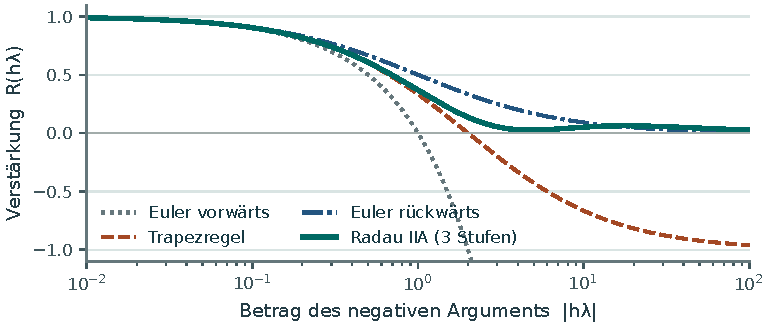
\includegraphics[width=.88\linewidth,height=49mm,keepaspectratio]{stabil.pdf}\par}\capline{Ein Schritt kann die physikalische Dämpfung umkehren.}
\seite{}{Explizite Einschrittverfahren}\anchorpage{2}{abs2-1}{2.1 · Runge–Kutta-Verfahren konstruieren}\ey{ABSCHNITT 2.1}\ptitle{Runge–Kutta-Verfahren konstruieren}
\hypertarget{punkt2-1-1}{}\subt{2.1.1\enspace Zwischenstufen als vorläufige Zustände}
Am beheizten Stab berechnet die erste Stufe die momentane Erwärmung. Mit ihr entwerfen wir einen Zwischenzustand, fragen das physikalische Modell dort erneut und verwenden die Antwort zum Fortschreiben. Die Zwischenzustände sind Versuchswerte. Nur der gewichtete Endwert gelangt in die gespeicherte Bahn.
\hypertarget{punkt2-1-2}{}\subt{2.1.2\enspace Butcher-Tableau und Ordnungsbedingungen}
Ein explizites Tableau speichert \(c_i=\sum_{j<i}a_{ij}\), die Stufen \(k_i=f(t_n+c_ih,y_n+h\sum_{j<i}a_{ij}k_j)\) und die Gewichte \(b_i\). Für konstantes Feld muss \(\sum b_i=1\) gelten. Für \(y'=t\) ist die Steigung linear, ihre exakte Fläche erzwingt \(\sum b_ic_i=1/2\). Ordnung drei verlangt zusätzlich \(b^Tc^2=1/3,\ b^TAc=1/6\), wobei \(c^2\) komponentenweise gilt. Die beiden Bedingungen unterscheiden Zeitkrümmung von einer geschachtelten Rückkopplung.
\hypertarget{punkt2-1-3}{}\subt{2.1.3\enspace Heun, Kutta dritter Ordnung und klassisches RK4}
Heun mittelt Startsteigung und Steigung am Euler-Endpunkt. Kutta-3 verwendet \(c=(0,1/2,1)\), Stufenzeilen \((1/2)\), \((-1,2)\) und Gewichte \((1,4,1)/6\). Bei RK4 folgen auf die Startsteigung zwei Mittelpunktssteigungen und eine Endsteigung. Die Gewichte sind \((1,2,2,1)/6\). Die vier Stufen am realen Heizmodell stehen auf S.\,\pagelink{zeit}. Für \(y'=-y,\ y_0=1,\ h=1\) liefern die drei Verfahren \(1/2,1/3,3/8\). Der Vergleichswert \(e^{-1}\) zeigt, weshalb ein guter erster Schritt noch keine beobachtete Ordnung beweist.
\seite{Rechenbeispiel}{Explizite Einschrittverfahren}\anchorpage{2}{kap4}{Wie baut man aus Steigungen einen Zeitschritt?}\ptitle{Wie baut man aus Steigungen einen Zeitschritt?}


\lernziel{Sie können Euler und Heun selbst ausführen und erklären, wann Genauigkeit, Stabilität oder der Aufwand eines impliziten Schritts die Solverwahl bestimmt.}
Ein Wagen ruht. Während der nächsten Sekunde nimmt seine Beschleunigung gleichmäßig von 0 auf \(2\unitm{m/s^2}\) zu. Was zeigt der Tacho am Ende? Zeichnen Sie die Beschleunigung über der Zeit. Die gesuchte Geschwindigkeitsänderung ist die Fläche unter der Geraden.
\subt{Zwei Rechenregeln, eine unabhängige Kontrolle}
Euler benutzt die Beschleunigung am Anfang. Der Beitrag ist \(1\unitm s\cdot0\unitm{m/s^2}=0\). Für Heun schätzen wir zunächst das Ende mit Euler, werten dort die Beschleunigung aus und mitteln beide Steigungen. Hier hängt die Beschleunigung nur von der Uhr ab. Der Mittelwert ist \((0+2)/2=1\unitm{m/s^2}\), also zeigt der Tacho \(1\unitm{m/s}\).

Die Dreiecksfläche ist unabhängig davon \(\tfrac12\cdot1\cdot2=1\unitm{m/s}\). Heun trifft sie in diesem Sonderfall genau, weil eine Gerade die beiden Messpunkte exakt verbindet. Beim Prüfwagen mit Luftwiderstand hängt die Steigung zusätzlich vom erreichten Tempo ab. Dort müssen wir den Fehler messen.
\notebox{Versuchen Sie einen kleineren Schritt}{Teilen Sie die Sekunde in zwei gleiche Teile. Welche Beschleunigungen sieht Euler an deren Anfängen? Aus \(0{,}5\cdot0+0{,}5\cdot1=0{,}5\unitm{m/s}\) wird sichtbar, was die zweite Auswertung verbessert und welcher Flächenanteil weiterhin fehlt.}
\subt{Wann lohnt die zusätzliche Rechnung?}
Bei einem steilen Abklingen kann ein zu großer Schritt eine abklingende Bewegung sogar wachsen lassen. Die spätere Kontrollrechnung vergleicht deshalb auch den Fehler und die Zahl der nötigen Auswertungen.

\srcs{\textbf{Kernweg}\enspace\see{zeit}{Euler, Heun und RK4}\quad\textbf{Vertiefung}\enspace\see{radau}{Radau-Kollokation}\quad\see{ueb4}{Selbst prüfen}. · \see{pyregler}{In Python ausführen}}

\lektion{Einen Schritt aus Steigungen bauen}{zeit}{Kernweg}{Zeitintegration}
\vorhersage{4}{Ein Wagen steht. Die Zugkraft beginnt bei null und wächst. Was meldet Euler nach seinem ersten Schritt?}{kontrolleA}
Halten Sie die Wärmebilanz des Stabs fest und ändern Sie nur die Schrittregel. Für den Temperaturüberschuss gilt \(\theta(0)=0,\ f(\theta)=(10-\theta/4)/120\). Euler übernimmt \(1/12\unitm{K/s}\) für die ganzen \(60\unitm s\). Das liefert \(5\unitm K\), exakt sind es \(4{,}700124\unitm K\). Die wachsende Wärmeabgabe macht die Anfangssteigung im Laufe des Schritts zu groß.
\subt{Zwischenwerte als Rechenhilfe}
Heuns Verfahren berechnet zuerst den Euler-Prädiktor \(5\unitm K\). Die dortige Steigung ist \((10-5/4)/120=0{,}0729167\unitm{K/s}\). Der Mittelwert aus Anfangs- und Endsteigung liefert \(4{,}6875\unitm K\). Das klassische Runge--Kutta-Verfahren vierter Ordnung (RK4) baut vier Steigungen auf.
{\tblstart\begin{tabularx}{\linewidth}{@{}lYrr@{}}\toprule
\hd{Stufe}&\hd{Auswertung}&\hd{Probezustand [K]}&\hd{Steigung [K/s]}\\\midrule
\(k_1\)& \(f(\theta_0)\)&0&0,08333333\\
\(k_2\)& \(f(\theta_0+hk_1/2)\)&2,500000&0,07812500\\
\(k_3\)& \(f(\theta_0+hk_2/2)\)&2,343750&0,07845052\\
\(k_4\)& \(f(\theta_0+hk_3)\)&4,707031&0,07352702\\\bottomrule
\end{tabularx}\par}
\[
 \theta_1=\theta_0+\frac h6(k_1+2k_2+2k_3+k_4)=4{,}700114\unitm K .
\]
Die zwei Probezustände am halben Schritt erfassen, wie sich die Steigung mit der Temperatur ändert.
\subt{Ein Butcher-Tableau lesen}
Allgemein gilt \(k_i=f(t_n+c_i h,\,y_n+h\sum_j a_{ij}k_j)\) und \(y_{n+1}=y_n+h\sum_i b_i k_i\). Bei RK4 sind \(c=(0,1/2,1/2,1)\), \(b=(1,2,2,1)/6\) und die einzigen von null verschiedenen Einträge \(a_{21}=a_{32}=1/2,\ a_{43}=1\). Die strikte untere Dreiecksform ermöglicht die Auswertung von oben nach unten.
\subt{Warum vier Stufen an der linearen Probe helfen}
Für \(y'=\lambda y\) liefert Einsetzen der vier Stufen den Faktor \(R_4(z)=1+z+z^2/2+z^3/6+z^4/24\), \(z=h\lambda\). Die Exponentialreihe stimmt bis zur vierten Potenz überein. Für dieses Testproblem beginnt der lokale Defekt mit \(z^5y_n/120\). Die allgemeine Ordnung vier für nichtlineare Systeme folgt aus den zusätzlichen RK-Ordnungsbedingungen.
\srcs{\refbk{ode}{Hairer, Nørsett und Wanner, Band I} · Vollständige Zahlen in der eingebetteten Datei \texttt{nachrechnen.py}.}

\lektion{Der Prüfwagen als ODE ohne elementare Lösung}{wagenmodell}{Kernweg}{Zeitintegration}
Ein Prüfwagen startet aus der Ruhe. Sein Antrieb erhöht die Zugkraft jede Sekunde um ein Newton. Gesucht ist die Geschwindigkeit nach einer Sekunde. Darf ein Schalter ansprechen, der \(0{,}48\unitm{m/s}\) verlangt? Ohne Widerstand ergäbe sich \(0{,}5\unitm{m/s}\). Ob uns diese Schätzung für den Schalter genügt, hängt vom Kraftgesetz ab.
\subt{Aus den Kräften zur Gleichung}
Wir modellieren den Wagen als Masse \(m=1\unitm{kg}\). Er fährt waagerecht vorwärts. Ein geschwindigkeitsabhängiger Widerstand wirkt der Bewegung entgegen und beträgt \(c\,v|v|\) mit \(c=1\unitm{kg/m}\). Mit \(\kappa=1\unitm{N/s}\) für die Kraftrampe folgt aus Kraft gleich Masse mal Beschleunigung
\[
 m\dot v=\kappa t-cv|v|,\qquad v(0)=0.
\]
Mit \(s=t/(1\unitm s)\) und \(y=v/(1\unitm{m/s})\) ergibt sich \(y'=s-y|y|\). Für \(s\ge0\) bleibt die Bahn nichtnegativ: Bei \(y=0\) ist die Steigung \(s\), nach dem Start wächst die Geschwindigkeit. Auf unserem Zeitintervall gilt damit \(y'=s-y^2\). Beim Pumpenbeispiel war die Rate allein durch die Uhrzeit bestimmt. Hier bestimmt der erreichte Zustand die nächste Steigung mit.
\subt{Zwei Handrechnungen für die erste halbe Sekunde}
Gehen wir vom Start bis \(s=0{,}5\). Euler übernimmt die Steigung am Start, \(k_1=0-0^2=0\), und erhält wieder \(y=0\). Heun prüft zusätzlich die Steigung am vorhergesagten Ende. Dort liefert \(k_2=0{,}5-0^2=0{,}5\). Aus beiden Steigungen folgt
\[
 y_{\rm Heun}=0+0{,}5\,\frac{0+0{,}5}{2}=0{,}125.
\]
Der Unterschied entsteht schon bei fehlerfrei ausgeführten Rechenoperationen. Während des Schritts wächst die Antriebskraft. Euler verwendet diese Information erst beim nächsten Schritt.
\notebox{Erst schätzen}{Mit Widerstand muss die Geschwindigkeit nach einer Sekunde unter \(0{,}5\unitm{m/s}\) liegen. Reicht diese einseitige Schranke für die Entscheidung bei \(0{,}48\unitm{m/s}\)? Prüfen Sie Ihre Vermutung mit der Tabelle auf der nächsten Seite.}
\srcs{\see{zeit}{Heuns Stufen} · \see{wagenreferenz}{Unabhängige Vergleichsrechnung} · \href{https://pi.math.cornell.edu/~hubbard/diffalg1.pdf}{Hubbard und Lundell, Gleichung (1)}.}

\lektion{Eine unabhängige Antwort für den Prüfwagen}{wagenreferenz}{Kernweg}{Zeitintegration}
Welchen Schalter würde jede der beiden Rechnungen freigeben? Beide bekommen denselben Start und dieselbe Antriebskraft. Die Linearisierung des Widerstands \(y|y|\) bei Ruhe hat Steigung null. Mit \(y'=s\) folgt \(y_\mathrm{lin}=s^2/2\). Die Tabelle stellt diesem Modell die Integration der vollständigen Gleichung gegenüber.
{\tblstart\begin{tabularx}{\linewidth}{@{}r r r r r Y@{}}\toprule
\hd{\(t\) [s]}&\hd{Heun 0,5 s}&\hd{Heun 0,25 s}&\hd{DOP853}&\hd{Referenz}&\hd{Linear}\\\midrule
0,5&0,12500&0,12379&0,12346&0,12346&0,12500\\
1&0,46239&0,45604&0,45554&0,45554&0,50000\\
2&1,16122&1,18695&1,19358&1,19358&2,00000\\\bottomrule\end{tabularx}\par}
Alle Ergebnisse sind Geschwindigkeiten in \(\mathrm{m/s}\). Nach einer Sekunde bleibt das nichtlineare Modell mit \(0{,}45554\unitm{m/s}\) unter der Schwelle. Die Linearisierung würde den Schalter freigeben. Der adaptive DOP853-Lauf verwendet \(\mathrm{rtol}=10^{-11}\), \(\mathrm{atol}=10^{-13}\) und höchstens \(0{,}1\unitm s\) je Schritt.
\subt{Woher die Referenzspalte kommt}
Für \(y=w'/w\) gilt \(y'=w''/w-y^2\). Also genügt es, \(w''=s\,w\) mit \(w(0)=1,\ w'(0)=0\) zu lösen. Dies ist die Airy-Gleichung. Ihre beiden unabhängigen Standardlösungen heißen \(\mathrm{Ai}\) und \(\mathrm{Bi}\). Die Kombination
\[
 W(s)=\mathrm{Bi}'(0)\mathrm{Ai}(s)-\mathrm{Ai}'(0)\mathrm{Bi}(s)
\]
erfüllt \(W'(0)=0,\ W(0)\ne0\). Somit ist \(w=W/W(0)\) und \(y=W'/W\). Für \(s\ge0\) bleibt \(w\) positiv: Solange \(w>0\), ist \(w''=sw\ge0\), also wächst \(w'\) ab null und \(w\) kann keinen ersten Nullpunkt erreichen.
\subt{Warum man die elementare Formel vergeblich sucht}
Für \(y'=s-y^2\) haben Hubbard und Lundell bewiesen, dass sich keine Lösung durch elementare Funktionen darstellen lässt. Ihr Satz schließt sogar weiter gefasste Ausdrücke mit wiederholter Integration und Exponentialbildung aus. Die Spezialfunktionen liefern hier eine exakte Referenz. Die Zeitrechnung kann dasselbe Kraftmodell auch dann weiterverwenden, wenn eine gemessene Kraftrampe die Funktion \(\kappa t\) ersetzt.
\srcs{\texttt{python labor.py wagen} · \href{https://pi.math.cornell.edu/~hubbard/diffalg1.pdf}{Hubbard und Lundell, Einleitung und Korollar 8.1} · \href{https://dlmf.nist.gov/9.2}{NIST DLMF, Airy-Gleichung}.}

\seite{}{Explizite Einschrittverfahren}\anchorpage{2}{abs2-2}{2.2 · Lokaler Fehler und eingebettete Paare}\ey{ABSCHNITT 2.2}\ptitle{Lokaler Fehler und eingebettete Paare}
\hypertarget{punkt2-2-1}{}\subt{2.2.1\enspace Vom lokalen Defekt zum globalen Fehler}
Starten wir auf der exakten Bahn, hinterlässt ein Verfahren der Ordnung \(p\) nach einem Schritt den Defekt \(O(h^{p+1})\). Ein vorhandener Fehler \(e_n\) wird zusätzlich transportiert. Gilt \(\|e_{n+1}\|\le(1+hL)\|e_n\|+Ch^{p+1}\), entsteht durch Aufsummieren einer geometrischen Reihe bei \(e_0=0\) die Schranke \(Ch^p(e^{LT}-1)/L\) für feste Endzeit \(T\) und \(L>0\). Halbieren der Schrittweite prüft diese Beziehung im glatten Problem.
\hypertarget{punkt2-2-2}{}\subt{2.2.2\enspace Zwei Endwerte aus denselben Stufen}
Zwei Gewichtszeilen bilden \(y_{n+1}\) und \(\hat y_{n+1}\) aus denselben ausgewerteten Steigungen. Die Differenz \(h\sum_i(b_i-\hat b_i)k_i\) schätzt im asymptotischen Bereich den führenden lokalen Fehler der niedrigeren Formel. Verschwindet dieser Term ausnahmsweise, kann der Schätzer die Schwierigkeit des folgenden Schritts unterschätzen.
\hypertarget{punkt2-2-3}{}\subt{2.2.3\enspace RK23, RK45 und DOP853 unterscheiden}
Bogacki–Shampine führt eine Lösung dritter Ordnung mit eingebetteter zweiter Ordnung fort. Dormand–Prince 5(4) liefert den verbreiteten RK45. DOP853 ist ein eigenes Verfahren achter Ordnung mit Schätzern fünfter und dritter Ordnung. Jede Formel besitzt eigene Koeffizienten und eine passende dichte Ausgabe. Tauscht man nur den Namen in einem Versuchsbericht aus, lässt sich seine Aufrufzahl kaum interpretieren.
\srcs{\href{https://docs.scipy.org/doc/scipy/reference/generated/scipy.integrate.solve_ivp.html}{SciPy, Löserverfahren und dichte Ausgaben} · \refbk{ode}{Hairer, Nørsett und Wanner}.}
\lektion{Vom lokalen zum globalen Fehler}{ordnung}{Vertiefung}{Zeitintegration}
Ein lokal aus der exakten Lösung gestarteter Euler-Schritt hat bei zweimal stetig differenzierbarer Lösung den Defekt
\[
 y(t+h)-y(t)-hf(t,y(t))=\frac{h^2}{2}y''(\xi),\qquad t<\xi<t+h
\]
für eine skalare Komponente. Ein Verfahren der Ordnung \(p\) hat unter den zugehörigen Glattheitsannahmen einen lokalen Schrittdefekt \(O(h^{p+1})\). Beim Durchmarsch über ein festes Intervall wird der Fehler aus jedem früheren Schritt mittransportiert.
\subt{Satz · Stabile Fehlerfortpflanzung kostet eine Ordnung}
Für eine Einschrittabbildung \(\Phi_h\) gelte \(\|\Phi_h(u)-\Phi_h(v)\|\le(1+Lh)\|u-v\|\) und für jeden exakten Start ein Defekt höchstens \(Kh^{p+1}\). Bei exaktem Anfangswert und \(nh\le T\) folgt
\[
 \|e_n\|\le \frac{K}{L}(e^{LT}-1)h^p\quad (L>0).
\]
\proofpart{Addieren und subtrahieren von \(\Phi_h(y(t_n))\) ergibt \(\|e_{n+1}\|\le(1+Lh)\|e_n\|+Kh^{p+1}\). Iteration ab \(e_0=0\) und Summation der geometrischen Reihe liefern \(Kh^p((1+Lh)^n-1)/L\). Wegen \(1+Lh\le e^{Lh}\) folgt die Schranke. Für \(L=0\) ergibt direktes Summieren \(KTh^p\).}
\subt{Ordnung beobachten}
Halbiert man bei festem Endzeitpunkt \(h\), so ergibt \(p_\mathrm{obs}=\log_2(E_h/E_{h/2})\) einen Schätzwert für die Ordnung. Dazu müssen dieselbe Messgröße, dieselbe Referenz und derselbe Endzeitpunkt verwendet werden. Für Euler, Heun und RK4 erwartet man an einem glatten ODE-Problem asymptotisch die Werte 1, 2 und 4.

In einer Stoßrechnung gilt die glatte Fehlerentwicklung nur innerhalb einer Flugphase. Wird der Stoß verspätet behandelt, beginnt die nächste Phase bereits mit einem anderen Anfangswert. Eine kleine lokale Fehlerschätzung ersetzt deshalb keinen Vergleich der Stoßzeiten.
\task{3}{Für \(\dot y=-y,\ y(0)=1\) führt Euler einen Schritt \(h=1\) oder zwei Schritte \(h=1/2\) aus. Berechnen Sie beide Endwerte und Fehler. Wie lautet die exakte Euler-Folge bis \(t=1\) für \(n\) Schritte?}

\lektion{Was eine adaptive Toleranz steuert}{adaptiv}{Kernweg}{Zeitintegration}
Ein eingebettetes Runge--Kutta-Paar nutzt dieselben Stufen mit zwei verschiedenen Endgewichten. Beim Bogacki--Shampine-Paar RK23 hat die fortgeschriebene Lösung Ordnung 3, die Vergleichslösung Ordnung 2. Für ihre Differenz gilt bei glatter Lösung typischerweise \(\delta\sim K h^3\).
\[
 \begin{array}{c|cccc}
 0&&&&\\
 1/2&1/2&&&\\
 3/4&0&3/4&&\\
 1&2/9&1/3&4/9&\\ \hline
 b^{(3)}&2/9&1/3&4/9&0\\
 b^{(2)}&7/24&1/4&1/3&1/8
 \end{array}
\]
Die letzte Stufe liegt am vorgeschlagenen Endzustand. Nach Annahme des Schritts kann die dortige Steigung beim nächsten Schritt wiederverwendet werden, solange die Modellgleichung und der Zustand stetig fortgesetzt werden.
\subt{Zwei Endwerte aus denselben Stufen}
Für \(y'=-y,\ y_0=1,\ h=1/2\) ergibt das Tableau \(k=(-1,-3/4,-23/32,-29/48)\). Einsetzen liefert \(y^{(3)}=1+\tfrac12(2k_1/9+k_2/3+4k_3/9)=29/48\) und \(y^{(2)}=1+\tfrac12(7k_1/24+k_2/4+k_3/3+k_4/8)=463/768\). Die Schätzung ist \(1/768\), die exakte Abweichung der fortgeschriebenen Lösung von \(e^{-1/2}\) beträgt etwa \(0{,}00236\). Bei absoluter Toleranz \(0{,}002\) nimmt der Schätzer den Schritt an.
\subt{Volt und Ampere gemeinsam skalieren}
Eine mögliche gewichtete Norm verwendet
\[
 s_i=\mathrm{atol}_i+\mathrm{rtol}\max(|y_{n,i}|,|y_{n+1,i}|),\qquad
 \eta=\sqrt{\frac1m\sum_{i=1}^m(\delta_i/s_i)^2}.
\]
Die absolute Toleranz hat die Einheit der jeweiligen Komponente, die relative Toleranz ist dimensionslos. Ein Regler akzeptiert etwa bei \(\eta\le1\) und setzt \(h_{\rm neu}\approx0{,}9h\,\eta^{-1/3}\) mit begrenzten Änderungsfaktoren. Bei \(\eta=8\) ergibt das \(0{,}45h\) für den neuen Versuch. Der Exponent kommt aus der dritten Potenz in der Fehlerschätzung.
\subt{Wann RK45 passt}
Dormand--Prince RK45 kombiniert die Ordnungen 5 und 4 für glatte, nichtsteife Probleme. Bei bekannten Sprüngen startet die Integration mit aktualisiertem Modell neu. Messfehler brauchen eine eigene Kontrolle.
\srcs{\refbk{paare}{Bogacki--Shampine und Dormand--Prince} · \refbk{scipy}{SciPy-Dokumentation zu den implementierten Paaren und ihrer dichten Ausgabe}.}

\seite{}{Explizite Einschrittverfahren}\anchorpage{2}{abs2-3}{2.3 · Schrittweitensteuerung und dichte Ausgabe}\ey{ABSCHNITT 2.3}\ptitle{Schrittweitensteuerung und dichte Ausgabe}
\hypertarget{punkt2-3-1}{}\subt{2.3.1\enspace Relative und absolute Fehlerskalen}
Ein Strom nahe null und eine Spannung von zehn Volt benötigen unterschiedliche absolute Fehlerbudgets. Mit \(s_i=\mathrm{atol}_i+\mathrm{rtol}\max(|y_i|,|y_i^+|)\) werden die Differenzen \(d_i\) dimensionslos. Ein verbreitetes Kriterium ist \(E=\sqrt{\sum_i(d_i/s_i)^2/n}\). Ein Maximaltest schützt jede Komponente einzeln. Die gewählte Norm gehört zur Beschreibung des Versuchs.
\hypertarget{punkt2-3-2}{}\subt{2.3.2\enspace I-, PI- und PID-Regelung}
Skaliert der Schätzer wie \(h^r\), folgt aus \(E(h_{neu}/h)^r\approx1\) der I-Vorschlag \(h_{neu}=\eta h E^{-1/r}\). Ein PI-Regler verbindet aktuellen und letzten akzeptierten Fehler, etwa \(h_{neu}/h=\eta E_n^{-0.7/r}E_{n-1}^{0.4/r}\). PID-Varianten nutzen weitere Fehlerhistorie. Nach einem Reset beginnt die Historie neu. Die Koeffizienten sind ein Reglerentwurf und müssen zur Schätzformel passen.

In Logarithmen wird die Wirkung der Historie lesbar. Setzen wir \(e_n=\log E_n\) für positive Fehler. Ein verbreiteter Aufbau kombiniert \(-\beta_1 e_n+\beta_2e_{n-1}-\beta_3e_{n-2}\) mit \(\log\eta\) zu \(\log(h_{n+1}/h_n)\). Exponenzieren liefert drei Fehlerfaktoren. Für den hier verwendeten PI-Fall ist \(\beta_3=0\). Ein PID-Entwurf kann zusätzlich auf eine Änderung des Fehlertrends reagieren. Die Auswahl der Koeffizienten hängt von Verfahren, Fehlerordnung und gewünschter Reglerdämpfung ab.
\hypertarget{punkt2-3-3}{}\subt{2.3.3\enspace Akzeptanz, Verwerfung und Grenzen}
Für \(E\le1\) werden die Kandidatenzeit und der Zustand übernommen. Bei Verwerfung bleiben Zeit, Zustand und akzeptierte Historie erhalten. Der nächste Versuch benutzt einen beschränkten kleineren Schritt. Bei \(E=0\) begrenzt ein Wachstumsfaktor die Vergrößerung. Liegt der notwendige Schritt unter der darstellbaren Zeitauflösung, endet der Lauf mit einer Diagnose. Ein fester Ausgabezeitpunkt ist kein Grund, den lokalen Fehlertest zu umgehen.
\hypertarget{punkt2-3-4}{}\subt{2.3.4\enspace Hermite- und Kollokationspolynome}
Die kubische Hermite-Kurve stimmt in Wert und Ableitung an beiden Schrittenden überein. Für \(s=(t-t_n)/h\) sind ihre Basisfunktionen \(2s^3-3s^2+1,\ s^3-2s^2+s,\ -2s^3+3s^2,\ s^3-s^2\). Sie multiplizieren \(y_n,h f_n,y_{n+1},h f_{n+1}\). Bei Kollokation integrieren wir stattdessen das Stufenpolynom. Beide liefern an Zwischenzeiten eine kontrollierbare Näherung. Kapitel 5 nutzt diese Kurve als Suchintervall für den Stoß.
\lektion{Einen Schritt annehmen oder verwerfen}{pyregler}{Solvertechnik}{Python}
Das Anfangswertproblem sammelt Gleichung, Startzeit, Startzustand und Endzeit. Das Projekt prüft beim Auswerten Dimension und Endlichkeit der zurückgegebenen Raten. Erst der Aufruf von \texttt{solve\_ivp} legt das Verfahren fest.
{\footnotesize\begin{verbatim}
from argesim_benchmarks.ivp import InitialValueProblem
from argesim_benchmarks.runtime import solve_ivp

p = InitialValueProblem(heizstab, 0.0, (0.0,), 60.0)
for name in ("euler", "rk4"):
    r = solve_ivp(p, name, options={"step": 60.0})
    print(name, r.final_state[0], r.stats.rhs_evaluations)
\end{verbatim}}
Für die unabhängige Kontrolle trennen wir die Variablen. Mit \(\theta(0)=0\) folgt \(\theta(t)=40(1-e^{-t/480})\) in Kelvin. Nach einer Minute erwarten wir \(4{,}700123897\unitm K\).
{\tblstart\begin{tabularx}{\linewidth}{@{}Yrrrr@{}}\toprule
\hd{Verfahren}&\hd{\(\theta(60)\) [K]}&\hd{angenommen}&\hd{verworfen}&\hd{Aufrufe}\\\midrule
Euler&5,000000&1&0&1\\
RK4&4,700114&1&0&4\\
RK45 adaptiv&4,700124&3&2&31\\\bottomrule
\end{tabularx}\par}
Für RK45 lauteten die Optionen \texttt{initial\_step=60.0}, \texttt{rtol=1e-8} und \texttt{atol=1e-10} als Einträge des Wörterbuchs \texttt{options}. Das eingebettete Paar schätzt den lokalen Fehler aus zwei Näherungen. Wird die skalierte Toleranz verfehlt, probiert der Solver von der letzten angenommenen Zeit einen kleineren Schritt. Der verworfene Zustand gehört zu keinem gespeicherten Messpunkt.

\subt{Wie erkennt man einen fehlerhaften Callback?}
Ein Zähler der Modellaufrufe darf zu Diagnosezwecken wachsen. Würde derselbe Code dabei eine Pumpe dauerhaft umschalten oder die Modelluhr erhöhen, hingen spätere Raten von verworfenen Versuchen ab. Prüfen Sie die Rate bei identischen Eingaben zweimal sowie die gespeicherten Zeiten separat.
\srcs{\cpcode{argesim_benchmarks/runtime.py}{Auswahl und Optionen} · \cpcode{argesim_benchmarks/solvers/explicit.py}{Schritte und Auswertungen} · \see{kap5}{DAE mit Residuum und konsistentem Start}.}

\lektion{Energie und Phase über viele Perioden}{verlet}{Vertiefung}{Zeitintegration}
Für die reibungsfreie Masse aus Kapitel 1 wählen wir Einheiten mit \(m=k_f=1\), \(F=0\). Aus \(q(0)=1,\ v(0)=0\) folgen \(q=\cos t,\ v=-\sin t\) und \(H=(q^2+v^2)/2=1/2\). Am Ende von etwa 16 Perioden sind Energiedrift und Zeitverschiebung getrennt beobachtbar.
\subt{Störmer--Verlet aus zwei Halbschritten der Kraft}
Zuerst setzt die Feder für einen halben Schritt ihren Impuls um. Dann bewegt sich die Masse mit der so bestimmten Geschwindigkeit. Am neuen Ort wirkt die Feder den zweiten halben Schritt:
\[
 v_{1/2}=v_n-\tfrac h2 q_n,\quad q_{n+1}=q_n+h v_{1/2},\quad
 v_{n+1}=v_{1/2}-\tfrac h2q_{n+1}.
\]
\textbf{Warum bleibt die Energie nahe am Sollwert?} Setzt man \(d=1-h^2/4,\ c=1-h^2/2\), hat der Schritt die Matrix \(\left[\begin{smallmatrix}c&h\\-hd&c\end{smallmatrix}\right]\). Wegen \(c^2+h^2d=1\) gilt exakt
\[
 d(cq+hv)^2+(-hdq+cv)^2=dq^2+v^2 .
\]
Für \(0<h<2\) ist diese quadratische Form positiv definit. Sie weicht von \(q^2+v^2\) nur um einen Term der Ordnung \(h^2\) ab. Vorwärts Euler multipliziert \(q^2+v^2\) dagegen in jedem Schritt mit \(1+h^2\).

{\tblstart\begin{tabularx}{\linewidth}{@{}Yrr@{}}\toprule
\hd{500 Schritte, \(h=0{,}2\)}&\hd{max. rel. Energiefehler}&\hd{Phasenfehler bei \(t=100\) [rad]}\\\midrule
Vorwärts Euler & \(3{,}29\cdot10^8\)& \(-1{,}30222\)\\
RK4 & \(4{,}42\cdot10^{-4}\)& \(-0{,}00131\)\\
Störmer--Verlet & \(1{,}00\cdot10^{-2}\)& \(+0{,}16909\)\\\bottomrule
\end{tabularx}\par}
Die Phase wird aus dem über alle Umdrehungen fortgesetzten Winkel \(\operatorname{atan2}(-v,q)\) bestimmt. In diesem Zeitfenster liefert RK4 die kleineren Fehler. Für Verlet gibt es darüber hinaus den bewiesenen zeitunabhängigen Einschluss durch die modifizierte Energie des linearen Oszillators. Ein gleich großer Schritt bedeutet bei beiden Methoden unterschiedliche Arbeit.
\srcs{\refbk{geom}{Hairer, Lubich und Wanner, Störmer--Verlet} · Eigener Rechenversuch \texttt{oszillator}.}

\werkblatt{2}{Selbst prüfen}{ueb4}{Schrittweite, Ordnung und Stabilität}

\merke{Ein kleiner Fehler bei einem Schritt und stabiles Abklingen über viele Schritte beantworten verschiedene Fragen. Beides lässt sich an einer bekannten Lösung prüfen.}
\subt{A · Zwei Algorithmen am selben Start}
Ein normiertes Signal erfüllt \(\dot z=-4z,\ z(0)=1\), Zeit in Sekunden. Rechnen Sie einen Schritt der Länge \(0{,}25\unitm s\) mit Euler und mit Heun. Zeichnen Sie beim Heun-Schritt einen Pfeil zum vorhergesagten Ende, bevor Sie die zweite Steigung auswerten. Vergleichen Sie beide Resultate mit \(e^{-1}\).
\subt{B · Ein Vorzeichen richtig deuten}
Ein Programm verwendet für dieselbe Gleichung \(h=0{,}4\unitm s\) oder \(h=0{,}6\unitm s\). Berechnen Sie jeweils den Faktor eines Euler-Schritts. Bei welcher Einstellung klingt der Betrag ab? Bei welcher bleiben auch alle Werte positiv? Erklären Sie, warum „stabil“ allein die Form der physikalischen Kurve nicht garantiert.
\subt{C · Eine Schrittweite aus Daten wählen}
Für eine andere glatte Aufgabe sind die absoluten Endfehler gegen eine unabhängige Referenz bei \(h=0{,}20;\ 0{,}10;\ 0{,}05\unitm s\) genau \(0{,}040;\ 0{,}010;\ 0{,}0025\) in der Ausgabeeinheit. Schätzen Sie die beobachtete Ordnung. Welcher der getesteten Schritte ist der größte, der die inklusive Fehlergrenze \(0{,}010\) erreicht? Was könnten Sie daraus über eine zweite Messgröße schließen?
\hilfe{In B genügt ein Faktor pro Schritt, um alle späteren Beträge zu beurteilen. Für C hilft die Potenzregel. Halbiert sich \(h\), dann verändert sich ein Fehler \(Ch^p\) um den Faktor \(2^p\).}

\schreibfeld

\srcs{\see{loesweg4}{Lösungswege A, B und C}\quad·\quad\see{kap4}{Zum Kapitelauftakt}.}

\werkblatt{2}{Lösungswege}{loesweg4}{Schrittweite, Ordnung und Stabilität}

\subt{A · Die zweite Steigung auswerten}
Die Startsteigung ist \(-4\). Euler ergibt \(1+0{,}25(-4)=0\). Heun nimmt dieselbe Null als \emph{vorhergesagten} Endwert. Dort ist die Steigung null. Mit der mittleren Steigung ergibt sich \(1+0{,}25(-4+0)/2=0{,}5\). Der exakte Endwert ist \(e^{-1}\approx0{,}367879\). Die absoluten Fehler betragen rund \(0{,}367879\) und \(0{,}132121\). In diesem Schritt liegt Heun näher an der Referenz.
\subt{B · Abklingen und Positivität einzeln prüfen}
Euler multipliziert mit \(1-4h\). Bei \(h=0{,}4\) ist das \(-0{,}6\). Die Folge wechselt das Vorzeichen, ihr Betrag wird mit jedem Schritt kleiner. Bei \(h=0{,}6\) ist der Faktor \(-1{,}4\), sodass der Betrag wächst. Keine der beiden Einstellungen hält die Werte durchgehend positiv. Dafür muss bei diesem Start \(0\le h<0{,}25\) gelten. Bei \(h=0{,}25\) wird die Folge genau null und bleibt lediglich nichtnegativ.
\subt{C · Eine Ordnung beobachten}
Beide Fehlerquotienten betragen vier. Aus \(2^p=4\) folgt die beobachtete Ordnung \(p=2\) für diese Daten und diese Größe. Der größte getestete zulässige Schritt ist \(0{,}10\unitm s\), da Gleichheit zugelassen war. Der größte der drei Schritte überschreitet das Budget, der kleinste schafft zusätzliche Reserve.
\notebox{Den Vergleich richtig lesen}{Eine andere Messgröße kann empfindlicher reagieren. Bei einem Schalter ist zusätzlich der Zeitpunkt des Übergangs zu prüfen. Eine beobachtete Ordnung aus drei Werten ist noch kein allgemeiner Konvergenzbeweis.}

\srcs{\see{ueb4}{Noch einmal selbst rechnen}\quad·\quad\see{schluss4}{Forschungsstand und Beweisfragen}.}

\kapschluss{2}{Fehlerschätzung ist Teil des Verfahrens}{schluss4}
\subt{Stand der Forschung}
Ranocha und Giesselmann untersuchen explizite Runge--Kutta-Verfahren mit residuenbasierten Fehlerschätzern und Schrittweitenregelung. Sie leiten für die analysierten Kombinationen Stabilitätsaussagen über den Regler her und vergleichen sie mit eingebetteten Fehlerschätzern. Die Wahl der Integrationsformel allein legt das Verhalten des adaptiven Algorithmus damit noch nicht fest.
\subt{Bewiesener Satz und Reichweite}
Auf S.\,\pagelink{ordnung} wurde aus einem lokalen Defekt \(O(h^{p+1})\) und einer Stabilitätsabschätzung der globale Fehler \(O(h^p)\) auf einem festen Zeitintervall hergeleitet. Beim Übergang über einen Stoß ist die dort vorausgesetzte glatte Taylorentwicklung im Allgemeinen nicht über das Ereignis hinweg gültig. Deshalb werden die glatten Phasen und die Lage des Übergangs getrennt geprüft.
\subt{Ergebnis der Nachuntersuchung}
Für den skalaren Regler mit Rate \(a\) und gleichem Startwert erfüllt der Fehler einer stetigen, stückweise differenzierbaren Näherung \(Y\) die Gleichung \(e^\prime=-ae+r\) mit \(r=Y^\prime-f(t,Y)\). Integration ergibt \(|e(t)|\le(1-e^{-at})\sup|r|/a\). Die Nachrechnung schließt den konkreten Fehler der sechs dichten Ausgabekurven auf ganzen Zeitintervallen ein.
\srcs{\see{befund4}{Nachweis und Ergebnis} · \href{https://doi.org/10.1007/s44207-024-00001-0}{Ranocha und Giesselmann (2024), Stability of step size control based on a posteriori error estimates}\enspace·\enspace\see{tracking}{Folgeregler}.}

\lektion{Gilt die Fehlerschranke auch zwischen Zeitpunkten?}{befund4}{Nachweise}{Nachweise zum Modell}
Der steife Folgeregler hat die exakte Lösung \(y(t)=\cos t-e^{-1000t}\). Die dichte Ausgabe eines RK45-, Radau- oder BDF-Schritts ist hier ein Polynom \(P(t)\) vom Grad höchstens fünf. Wir können seinen größten Fehler auf dem \emph{ganzen} Schritt nach oben begrenzen. Dafür brauchen wir die vom Solver gespeicherten Polynomkoeffizienten.
\subt{Von sechs Prüfstellen zur ganzen Kurve}
Teile einen Schritt in Intervalle der Breite \(h\). Interpoliere auf jedem Teilintervall den Fehler \(e=P-y\) an sechs äquidistanten Punkten durch ein Polynom \(B\) vom Grad fünf. Seine Bernstein-Darstellung ist eine gewichtete Summe von sechs Koeffizienten, deren Basisgewichte überall nichtnegativ sind und zusammen eins ergeben. Also gilt \(|B|\le\max_j |b_j|\). Die Interpolationsrestformel ergibt ab dem linken Rand \(a\)
\[
 \sup |P-y|\le \max_j|b_j|+
             \frac{h^6}{720}\bigl(1+1000^6e^{-1000a}\bigr).
\]
Denn \(P^{(6)}=0\); das Produkt der sechs Abstände zu den Stützstellen ist höchstens \(h^6\). Der Rechenlauf wertet auch die Koeffizienten und den Restterm mit nach außen gerundeter Intervallarithmetik aus.
{\tblstart\begin{tabularx}{\linewidth}{@{}Yrr@{}}\toprule
\hd{Solver}&\hd{Obere Grenze bei \(\mathrm{rtol}=10^{-3}\)}&\hd{bei \(\mathrm{rtol}=10^{-6}\)}\\\midrule
RK45&\(2{,}22\cdot10^{-3}\)&\(1{,}19\cdot10^{-6}\)\\
Radau&\(2{,}04\cdot10^{-3}\)&\(2{,}30\cdot10^{-5}\)\\
BDF&\(5{,}44\cdot10^{-4}\)&\(1{,}10\cdot10^{-6}\)\\\bottomrule\end{tabularx}\par}
Die groben Läufe überschreiten das Ziel \(10^{-4}\) bereits an einzelnen Prüfstellen. Für die drei feinen Läufe liegen die oberen Schranken auf dem gesamten Intervall von 0 bis 2 s unter dem Ziel. Die Aussage bezieht sich auf die reellen Polynome aus den gespeicherten Binärkoeffizienten von SciPy 1.17.0. Die erneute Gleitkommaauswertung an einem Gerät kann zusätzlich runden.
\notebox{Übertragen}{Eine garantierte obere Grenze oberhalb des Ziels allein beweist keinen Fehlschlag. Welcher Befund genügt? Ein einziger nachweislich zu großer Punktfehler. Die Datei enthält zu jedem Lauf beide Grenzen.}
\srcs{\see{tracking}{Ursprünglicher Vergleich} · \texttt{kapitel.json}, Abschnitt \texttt{dense}.}
\lektion{Wie ein Regler nach einem Fehlversuch weiterrechnet}{pruefung2}{Herleitung und Gegenprobe}{Kapitel 2}
Eine steile Flanke tritt zwischen zwei geplanten Ausgaben auf. Ein eingebettetes RK-Paar liefert zwei Endwerte aus denselben Stufen. Ihre Differenz \(d\) misst, wie stark sich die beiden Näherungen bei der gewählten Schrittweite trennen. Für die folgende Handrechnung skaliere der Schätzer wie \(h^3\), wie bei einem üblichen 3(2)-Paar in einem glatten Bereich.

Nehmen wir \(E=8\) beim ersten Versuch mit \(h=0{,}1\unitm s\) an. Ein I-Regler mit Sicherheitsfaktor \(0{,}9\) schlägt \(h_{\rm neu}=0{,}1\cdot0{,}9/8^{1/3}=0{,}045\unitm s\) vor. Die neue Schätzung lautet bei gleichbleibendem Fehlerkoeffizienten \(8(0{,}045/0{,}1)^3=0{,}729\). Erst die neu berechneten Stufen entscheiden, ob diese Vorhersage zutrifft. Nach der Annahme darf der Regler \(0{,}729\) als Gedächtniswert verwenden. Die abgewiesene Acht würde den nächsten PI-Vorschlag verfälschen.

Wozu braucht man eine Norm? Für vier Komponenten mögen die bereits durch ihre physikalisch passenden Skalen geteilten Differenzen \((1{,}8,0,0,0)\) betragen. Das quadratische Mittel liefert \(\sqrt{1{,}8^2/4}=0{,}9\), der Maximalwert beträgt \(1{,}8\). Die Entscheidung hängt also auch davon ab, ob jede Komponente einzeln geschützt werden soll. Eine Schaltzeit mit eigenem Budget prüft man anschließend in Sekunden.

\notebox{Achtung, Falle}{Die RMS-Skalierung im Projektmodul \texttt{embedded23.py} gehört dort zu einem I-Regler mit Exponent \(-1/3\). Das PI-Schema auf der folgenden Werkstattseite ist eine alternative Implementierung mit denselben lokalen Fehlerdaten. Am festen Ausgaberaster darf man die Anzahl der verworfenen Versuche nicht ablesen.}
\srcs{\repocurrent{argesim_benchmarks/solvers/embedded23.py}{RK- und ESDIRK-3(2) im Projekt} · \see{alg2}{Regler mit Initialisierung und Wiederholung}.}

\lektion{Ein adaptiver Schritt als Entscheidung}{alg2}{Werkstatt}{Kapitel 2}
Der folgende Regler übernimmt den höherwertigen Kandidaten, sobald sein skalierter lokaler Fehler zulässig ist. \(r\) bezeichnet den Exponenten des Fehlerschätzers. Zu Beginn und nach jedem Modellwechsel ist \texttt{vorher} leer. \texttt{clip} beschränkt seinen ersten Wert auf das angegebene Intervall.
{\small\begin{verbatim}
solange t < ziel:
    h = min(h, h_max, ziel - t)
    wenn t + h <= t: melde fehlenden Zeitfortschritt
    hoch, tief = eingebettetes_paar(t, y, h)
    E = rms((hoch - tief) / skala(y, hoch))
    wenn E nicht endlich oder E > 1:
        wenn h <= h_min: beende mit Toleranzdiagnose
        f = 0.2 falls E nicht endlich sonst 0.9 * E**(-1/r)
        h = max(h_min, h * clip(f, 0.2, 0.9))
        wiederhole ohne Aenderung von t, y und vorher
    f = 5 falls E == 0 sonst 0.9 * E**(-1/r)
    wenn E > 0 und vorher vorhanden:
        f = 0.9 * E**(-0.7/r) * vorher**(0.4/r)
    t, y = t + h, hoch
    vorher = max(E, sehr_kleine_positive_Zahl)
    h = max(h_min, h * clip(f, 0.2, 5))
\end{verbatim}}
Der erfolgreiche Schlussversuch darf kürzer als \(h_{\min}\) sein. Für die RMS-Skala benötigen alle Komponenten positive Nenner. Bei einer verworfenen Stufe gehören auch neue Ausgaben und Ereignisse weiter zum vorläufigen Versuch.
\subt{Selbst rechnen}
Ein Paar mit quadratisch skalierendem Schätzer meldet E=4. Welche Änderung verlangt der reine I-Regler bei Sicherheitsfaktor 0,9?
\notebox{Lösung}{Der Versuch wird verworfen. Der neue Schritt beträgt 0,9 mal vier hoch minus ein Halb, also 0,45 des alten. Bei vergleichbarer Krümmung erwartet man nun einen normierten Fehler von etwa 0,81. Ein weiterer Fehlertest entscheidet über die Annahme.}

\seite{}{Implizite Integratoren}\anchorpage{1}{neu3}{3 · Implizite Integratoren, Radau IIA und BDF}\ey{KAPITEL 3}\ptitle{Implizite Integratoren, Radau IIA und BDF}
Der schnelle Wärmeausgleich ist vorüber. Der Stab nähert sich seinem Gleichgewicht jetzt gemächlich. Trotzdem verwirft ein expliziter Solver lange Schritte. Lohnt sich eine aufwendigere Gleichung pro Schritt, wenn sie die abgeklungene Mode zuverlässig dämpft?
\subt{Der Weg durch das Kapitel}
{\tblstart\begin{tabularx}{\linewidth}{@{}Yr@{}}\toprule
\hyperlink{abs3-1}{3.1 · Stabilität in der komplexen Ebene} & \pagelink{abs3-1}\\[2pt]
\hyperlink{abs3-2}{3.2 · Nichtlineare Gleichungen im Integrationsschritt} & \pagelink{abs3-2}\\[2pt]
\hyperlink{abs3-3}{3.3 · Radau IIA aus der Kollokation} & \pagelink{abs3-3}\\[2pt]
\hyperlink{abs3-4}{3.4 · Rückwärtsdifferenzen und variable Ordnung} & \pagelink{abs3-4}\\[2pt]
\bottomrule\end{tabularx}\par}
\par\vfill{\centering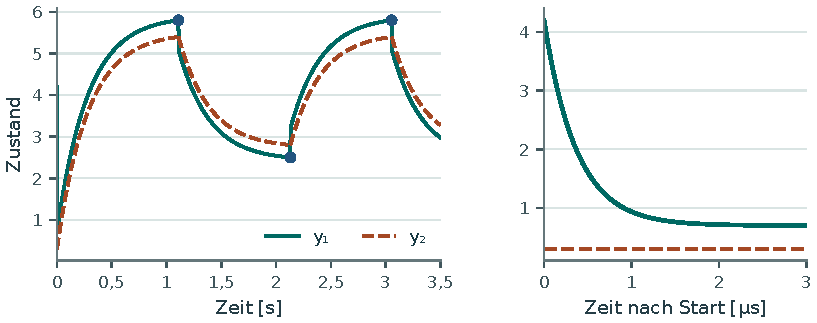
\includegraphics[width=.88\linewidth,height=49mm,keepaspectratio]{c05.pdf}\par}\capline{C05 hat auch nach dem schnellen Einschwingen eine messbare Schaltzeit.}
\seite{}{Implizite Integratoren}\anchorpage{2}{abs3-1}{3.1 · Stabilität in der komplexen Ebene}\ey{ABSCHNITT 3.1}\ptitle{Stabilität in der komplexen Ebene}
\hypertarget{punkt3-1-1}{}\subt{3.1.1\enspace Stabilitätsgebiete lesen}
Für \(y'=\lambda y\) wird aus einem Schritt die Multiplikation mit \(R(z)\), \(z=h\lambda\). Euler liefert \(1+z\). Die Randlinie \(|1+z|=1\) ist ein Kreis um \(-1\) mit Radius eins. Rückwärts-Euler löst \(y^+=y+h\lambda y^+\) und liefert \(R=1/(1-z)\). Ein imaginärer Anteil in \(\lambda\) bedeutet Rotation. Ein Abgleich nur auf der negativen reellen Achse übersieht sie.
\hypertarget{punkt3-1-2}{}\subt{3.1.2\enspace A-, Sektor- und L-Stabilität}
Eine A-stabile Einschrittmethode besitzt \(|R(z)|\le1\) auf der gesamten abgeschlossenen linken Halbebene. Bei \(A(\alpha)\)-Stabilität genügt dort ein Sektor mit Halbwinkel \(\alpha\) um die negative reelle Achse. L-Stabilität verlangt zusätzlich \(R(z)\to0\) für sehr große steife Argumente in der linken Halbebene. Die Trapezregel liefert bei \(z=-100\) den Faktor \(-49/51\), Rückwärts-Euler dagegen \(1/101\). Das Vorzeichen und die Größe erklären das numerische Nachschwingen im ersten Fall.
\notebox{Rechenfrage}{Bei welchem der beiden Ergebnisse ist die schnelle Mode nach zwei Schritten noch fast so groß wie zu Beginn? Quadrieren Sie beide Faktoren.}
\lektion{Rechenversuch · Ein steifer Folgeregler}{tracking}{Kernweg}{Zeitintegration}
Ein normierter Ausgang \(y\) soll einer Führungsgröße \(r(t)=\cos t\) folgen. Eine Vorsteuerung liefert \(\dot r\), eine Rückkopplung korrigiert den Abstand mit Rate \(a=1000\). Dadurch gilt \(\dot y=\dot r+a(r-y),\ y(0)=0\). Für den Folgefehler folgt \((y-r)'=-a(y-r)\). Somit ist \(y(t)=\cos t-e^{-1000t}\) eine unabhängige Referenz. Die Anfangsschicht dauert Millisekunden, der Versuch läuft bis \(2\unitm s\) bei \(t\) in Sekunden.

Alle Läufe verwenden dieselbe Gleichung und \(\mathrm{atol}=\mathrm{rtol}/100\). Für Radau und BDF ist \(J=[-1000]\) vorgegeben. \(E\) ist der größte Betrag des Fehlers der dichten Ausgabe auf einem gemeinsamen Gitter mit zusätzlicher Auflösung in der Anfangsschicht. Das Ziel ist \(E\le10^{-4}\).
{\tblstart\begin{tabularx}{\linewidth}{@{}Yrrrrr@{}}\toprule
\hd{Solver}&\hd{rtol}&\hd{Schritte}&\hd{\(f\)-Aufrufe}&\hd{LU}&\hd{\(E\)}\\\midrule
RK45 & \(10^{-3}\)&610&4226&0&\(1{,}19\cdot10^{-3}\)\\
RK45 & \(10^{-6}\)&731&4394&0&\(7{,}31\cdot10^{-7}\)\\
Radau & \(10^{-3}\)&14&100&28&\(2{,}02\cdot10^{-3}\)\\
Radau & \(10^{-6}\)&56&410&50&\(2{,}12\cdot10^{-5}\)\\
BDF & \(10^{-3}\)&56&144&19&\(5{,}40\cdot10^{-4}\)\\
BDF & \(10^{-6}\)&125&256&28&\(1{,}07\cdot10^{-6}\)\\\bottomrule
\end{tabularx}\par}
\subt{Wie liest man den Vergleich?}
Alle drei feinen Läufe erreichen das gemeinsame Ziel. Keiner der groben Läufe erreicht es. Der feine Radau-Lauf braucht die wenigsten angenommenen Schritte. Der feine BDF-Lauf benötigt weniger Funktionsaufrufe und Faktorisierungen als der feine Radau-Lauf. Der explizite RK45-Lauf hat den kleinsten gemessenen Fehler und die meisten Funktionsaufrufe. Die Rangfolge hängt also von der Messgröße und vom Aufwand pro Operation ab.

Die Gitterpunkte sind die Vereinigung aus \(0\), 501 logarithmischen Zeiten von \(10^{-7}\) bis \(0{,}03\) und 2001 äquidistanten Zeiten von 0 bis 2. Zwischen diesen Punkten kann der Fehler größer sein. Hier wird keine Maximalfehlergarantie und keine Laufzeitrangfolge aus den Zählern abgeleitet.
\srcs{Neu gerechneter Lehrversuch · NumPy 2.3.5, SciPy 1.17.0 · \texttt{nachrechnen.py}, Funktion \texttt{tracking}.}

\seite{}{Implizite Integratoren}\anchorpage{2}{abs3-2}{3.2 · Nichtlineare Gleichungen im Integrationsschritt}\ey{ABSCHNITT 3.2}\ptitle{Nichtlineare Gleichungen im Integrationsschritt}
\hypertarget{punkt3-2-1}{}\subt{3.2.1\enspace Das Newton-Verfahren für Stufengleichungen}
Für Rückwärts-Euler suchen wir die Nullstelle \(G(Y)=Y-y_n-hf(t_n+h,Y)\). Eine Korrektur \(\delta\) soll \(G(Y+\delta)\approx G(Y)+(I-hJ)\delta=0\) erfüllen. Lösen, addieren und neu auswerten ergibt Newton. Beim Beispiel \(y'=-y^2,y_n=h=1\) lautet die Gleichung \(Y^2+Y-1=0\). Aus \(Y=1\) folgt \(\delta=-1/3\), der neue Defekt beträgt nur noch \(1/9\).
\hypertarget{punkt3-2-2}{}\subt{3.2.2\enspace Analytische und numerische Jacobi-Matrizen}
Spalte \(j\) lässt sich über \([f(Y+\epsilon e_j)-f(Y)]/\epsilon\) annähern. Ein sehr großes \(\epsilon\) mittelt die Krümmung, ein sehr kleines verliert Ziffern durch Auslöschung. Eine analytische Ableitung lässt sich mit einem gerichteten Differenzenquotienten an mehreren Zuständen kontrollieren. Ein bekanntes Besetzungsmuster verringert die Arbeit bei großen Gittern.
\hypertarget{punkt3-2-3}{}\subt{3.2.3\enspace Modifiziertes Newton-Verfahren und LU-Wiederverwendung}
Hält man \(J\) im Schritt fest, kann der Solver \(P(I-hJ)=LU\) einmal faktorisieren. Jede Korrektur kostet dann zwei Dreieckslösungen. Das Protokoll unterscheidet Funktionsaufrufe, neue Matrizen, Faktorisierungen und Rücksetzungen. Stagniert das skalierte Residuum, wird die Matrix erneuert oder der Schritt wiederholt. Eine Änderung von \(h\) verändert die Newton-Matrix auch bei unverändertem \(J\).
\lektion{Die Algebra hinter impliziten Schritten}{algebra}{Kernweg}{Zeitintegration}
Beim Vorwärtsschritt kennen wir die Steigung am alten Zustand. Rückwärts Euler verlangt die Steigung am gesuchten neuen Zustand \(Y\). Es entsteht die Gleichung \(G(Y)=Y-y_n-hf(t_{n+1},Y)=0\). \emph{Implizit} bezeichnet hier die Zeitformel. Das zugrunde liegende Modell kann trotzdem eine explizite ODE sein.
\subt{Ein Newton-Schritt im Zahlenbeispiel}
Für \(\dot y=-y^2,\ y_n=1,\ h=0{,}1\) lautet \(G=Y+0{,}1Y^2-1\). Mit Startschätzung \(Y_0=1\) sind \(G(Y_0)=0{,}1\), \(G'(Y_0)=1{,}2\). Newton ergibt \(Y_1=1-0{,}1/1{,}2=0{,}916667\). Das neue Residuum ist etwa \(6{,}94\cdot10^{-4}\). Die positive Lösung der quadratischen Gleichung beträgt etwa \(0{,}916080\). Der exakte ODE-Wert ist \(1/1{,}1=0{,}909091\). Selbst eine bis auf Rundung gelöste Zeitformel hat noch Diskretisierungsfehler.

Bei mehreren Komponenten löst Newton \(J_G\,\Delta Y=-G\). Die \emph{LU-Zerlegung} faktorisiert die Matrix, gegebenenfalls nach Zeilenvertauschungen, in eine untere und eine obere Dreiecksmatrix. Bei gleicher Matrix können mehrere rechte Seiten mit denselben Faktoren durch Vorwärts- und Rückwärtseinsetzen gelöst werden. Die Zahl der Funktionsauswertungen und die Zahl solcher Faktorisierungen messen verschiedene Arten von Aufwand.
\subt{Wie aus Steigungen eine Kurve wird}
Eine \emph{Interpolation} wählt eine Funktion, die vorgegebene Werte an ausgewählten Punkten trifft. Für Punkte \(c_i\) ist \(\ell_j(c)=\prod_{i\ne j}(c-c_i)/(c_j-c_i)\) am Knoten \(c_j\) eins und an allen anderen Knoten null. Ein Polynom \(p(c)=\sum_j p_j\ell_j(c)\) nimmt so den Wert \(p_j\) bei \(c_j\) an. Bei der \emph{Kollokation} verlangt man von einem Ansatzpolynom, dass es die Differentialgleichung an bestimmten Knoten erfüllt. Radau IIA verwendet genau diese Idee.
\srcs{\refbk{stiff}{Hairer und Wanner, implizite Verfahren}\enspace·\enspace\see{radau}{Kollokationsrechnung für Radau IIA}.}

\seite{}{Implizite Integratoren}\anchorpage{2}{abs3-3}{3.3 · Radau IIA aus der Kollokation}\ey{ABSCHNITT 3.3}\ptitle{Radau IIA aus der Kollokation}
\hypertarget{punkt3-3-1}{}\subt{3.3.1\enspace Gauß-, Radau- und Lobatto-Knoten}
Eine Ersatzkurve soll an ausgewählten Punkten der Modellgleichung folgen. Gauß-Knoten liegen im Inneren, bei Radau ist ein Randpunkt enthalten, bei Lobatto beide. Für die rechte Radau-Variante ist die letzte Stufe eine Rechnung am Schrittende. Ihre Lage und die Gewichte bestimmen gemeinsam das Verhalten bei einer Bindung.
\hypertarget{punkt3-3-2}{}\subt{3.3.2\enspace Drei Stufen, fünfte Ordnung}
Für \(r=\sqrt6\) sind \(c_1=(4-r)/10, c_2=(4+r)/10, c_3=1\). Zu diesen Knoten seien \(\ell_j\) die Lagrange-Basispolynome. Integrieren der interpolierten Ableitung liefert \(a_{ij}=\int_0^{c_i}\ell_j(s)\,ds\), \(b_j=\int_0^1\ell_j(s)\,ds\). Das Tableau lautet
\[
\begin{array}{c|ccc}
c_1&(88-7r)/360&(296-169r)/1800&(-2+3r)/225\\
c_2&(296+169r)/1800&(88+7r)/360&(-2-3r)/225\\
1&(16-r)/36&(16+r)/36&1/9\\\hline
 &(16-r)/36&(16+r)/36&1/9
\end{array}
\]
Die Radau-Quadratur mit drei Knoten integriert Polynome bis Grad vier exakt. Die zugehörige Kollokationsmethode hat für hinreichend glatte ODEs globale Ordnung fünf.
\hypertarget{punkt3-3-3}{}\subt{3.3.3\enspace Stiff Accuracy und algebraische Bindungen}
Da \(a_{3j}=b_j\), ist der berechnete Endwert exakt der letzten Stufe gleich. Dies heißt \emph{stiffly accurate}. Eine in der Stufe gelöste Bindung geht damit bis zur Lösertoleranz in den Endwert ein. Eine Endstufe bei \(c_s=1\) allein garantiert das Gleichsetzen der Gewichte noch nicht. Die zugrunde liegende DAE muss regulär und passend initialisiert sein.
\lektion{Radau IIA aus einer Kollokationsidee}{radau}{Vertiefung}{Zeitintegration}
Können wir eine Kurve für den ganzen Schritt suchen und ihre Steigung an mehreren Stellen prüfen? Das dreistufige Radau-IIA-Verfahren wählt ein Polynom \(p\) vom Grad höchstens drei auf \([t_n,t_n+h]\) mit \(p(t_n)=y_n\). An den drei Prüfstellen muss die Steigung des Polynoms die Modellgleichung erfüllen.
\[
 p'(t_n+c_i h)=f(t_n+c_i h,p(t_n+c_i h)),\quad
 c_{1,2}=(4\mp\sqrt 6)/10,\quad c_3=1 .
\]
Interpolieren die Lagrange-Polynome \(\ell_j\) auf diesen drei Knoten die Stufensteigungen, so liefert Integration \(a_{ij}=\int_0^{c_i}\ell_j(s)\dg s\) und \(b_j=\int_0^1\ell_j(s)\dg s\). Weil \(c_3=1\), ergibt die letzte Stufe bereits den Endzustand. Diese Eigenschaft heißt \emph{stiffly accurate}. Das klassische dreistufige Verfahren besitzt für glatte ODEs globale Ordnung 5.
\subt{Dämpfung am Testproblem}
Für dieses Radau-Verfahren ist die Stabilitätsfunktion
\[
 R(z)=\frac{1+\frac25z+\frac1{20}z^2}
 {1-\frac35z+\frac3{20}z^2-\frac1{60}z^3}.
\]
Das Verfahren ist A-stabil. Der höhere Nennergrad erklärt darüber hinaus den Grenzwert null und damit die L-Stabilität. Bei \(z=-10\) liefert Radau \(0{,}05172\), rückwärts Euler \(0{,}09091\) und die Trapezregel \(-0{,}66667\). Die exakte Verstärkung beträgt \(e^{-10}=0{,}0000454\). Ein stabiler großer Schritt kann also für eine interessierende Anfangsschicht immer noch zu grob sein.
\subt{Wofür bezahlt man?}
Die unbekannten Stufen \(Y_i=y_n+h\sum_j a_{ij}f_j\) sind gekoppelt. Newton-Schritte verwenden Blöcke vom Typ \(\delta_{ij}I-h a_{ij}J_j\) mit \(J_j=\partial f/\partial y\). Lineare Algebra, Skalierung und Wiederverwendung von Faktorisierungen beeinflussen die Kosten. Bei großen räumlichen Gittern macht die dünn besetzte Jacobi-Matrix einen wesentlichen Unterschied.
\notebox{Implementierung}{SciPys \texttt{Radau} integriert eine ODE in der Form \(\dot y=f(t,y)\). Für eine allgemeine Residual-DAE braucht man eine Schnittstelle, die \(F(t,y,\dot y)=0\) entgegennimmt. Diese Unterscheidung wird auf S.\,\pagelink{indexeins} durchgerechnet.}
\srcs{\refbk{stiff}{Hairer und Wanner} · \refbk{scipy}{SciPy Radau} · \refbk{radtab}{Koeffizienten und Stabilitätsfunktion}.}

\seite{}{Implizite Integratoren}\anchorpage{2}{abs3-4}{3.4 · Rückwärtsdifferenzen und variable Ordnung}\ey{ABSCHNITT 3.4}\ptitle{Rückwärtsdifferenzen und variable Ordnung}
\hypertarget{punkt3-4-1}{}\subt{3.4.1\enspace BDF1 bis BDF6 konstruieren}
Der Integrator besitzt bereits frühere Zustände. Legen wir ein Polynom durch den gesuchten neuen Wert und \(k\) frühere Werte und differenzieren es am neuen Ende, entsteht bei konstantem Schritt \(h f_{n+1}=\sum_{j=0}^k\alpha_j y_{n+1-j}\). Die folgende Tabelle gibt die Zähler in zeitlich rückwärts laufender Reihenfolge an. Division durch den letzten Spaltenwert ergibt alle \(\alpha_j\).
{\tblstart\begin{tabularx}{\linewidth}{@{}rYr@{}}\toprule
\hd{Ordnung}&\hd{Zähler ab dem neuen Zustand}&\hd{Teiler}\\\midrule
1&1, \ensuremath{-}1&1\\2&3, \ensuremath{-}4, 1&2\\3&11, \ensuremath{-}18, 9, \ensuremath{-}2&6\\4&25, \ensuremath{-}48, 36, \ensuremath{-}16, 3&12\\5&137, \ensuremath{-}300, 300, \ensuremath{-}200, 75, \ensuremath{-}12&60\\6&147, \ensuremath{-}360, 450, \ensuremath{-}400, 225, \ensuremath{-}72, 10&60\\\bottomrule\end{tabularx}\par}
Setzen Sie eine konstante Kurve ein. Jede Zeilensumme ergibt null. Setzen Sie danach eine Gerade ein. Die Formel muss ihre Steigung liefern. Variable Schrittweiten erfordern neu bestimmte Differenzengewichte.
\hypertarget{punkt3-4-2}{}\subt{3.4.2\enspace Dahlquist-Barrieren und Ordnungswechsel}
Für ein konvergentes A-stabiles lineares Mehrschrittverfahren ist die Ordnung höchstens zwei. BDF1 und BDF2 sind A-stabil, die Ordnungen drei bis sechs besitzen kleinere Stabilitätssektoren. Ab BDF7 scheitert bereits die Nullstabilität der klassischen konstanten Schrittfolge. Ein adaptiver Solver vergleicht Fehler- und Kostenschätzungen benachbarter Ordnungen. Er braucht genügend glatte Historie, um höher zu schalten. Ein Stoß erzwingt deren Neustart. Die SciPy-Implementierung nutzt die Ordnungen eins bis fünf.
\srcs{\href{https://docs.scipy.org/doc/scipy/reference/generated/scipy.integrate.BDF.html}{SciPy BDF} · \refbk{ode}{Hairer, Nørsett und Wanner}.}
\lektion{Wie BDF, ESDIRK und Rosenbrock einen Schritt berechnen}{bdf}{Vertiefung}{Zeitintegration}
\subt{BDF2 verwendet einen früheren Zustand}
Eine BDF (Backward Differentiation Formula) approximiert die neue Steigung mit zurückliegenden Werten. Die Ableitung des quadratischen Interpolationspolynoms durch \(y_{n-1},y_n,y_{n+1}\) am neuen Zeitpunkt ergibt bei konstanter Schrittweite
\[
 \frac{3y_{n+1}-4y_n+y_{n-1}}{2h}=f(t_{n+1},y_{n+1}).
\]
Für \(y'=-ay\) wird daraus \((3+2ha)y_{n+1}=4y_n-y_{n-1}\). Bei einem nichtlinearen Modell muss pro Schritt eine nichtlineare Gleichung gelöst werden. Das Verfahren nutzt die Vorgeschichte. Ein Starter, etwa rückwärts Euler, erzeugt den fehlenden Anfangswert. Nach einem Zustandsreset muss die Historie passend neu aufgebaut werden.

BDF1 und BDF2 sind A-stabil. Höhere klassische BDF-Ordnungen besitzen eingeschränkte Stabilitätssektoren. Produktionssolver variieren Ordnung und Schrittweite. Für glatte lange Abschnitte kann sich diese Historie lohnen. Bei häufigen Neustarts oder genauer Ereigniszeit lohnt ein Vergleich mit Radau.
\subt{ESDIRK löst die Stufen nacheinander}
Beim explizit gestarteten, einfach diagonalen impliziten RK-Verfahren ist die erste Stufe explizit, die folgenden haben denselben Diagonalkoeffizienten \(\gamma\). Die untere Dreiecksstruktur erlaubt nacheinander kleinere nichtlineare Lösungen. Bei vereinfachtem Newton und festgehaltener Jacobi-Matrix lässt sich \(I-h\gamma J\) innerhalb eines Schritts wiederverwenden. Das eingebettete ESDIRK-3(2)-Paar der Studie kombiniert diese Struktur mit einer Fehlerkontrolle.
\subt{Rosenbrock linearisiert bereits im Verfahren}
Beim Rosenbrock--Euler-Schritt eines autonomen Systems löst man \((I-hJ_n)k=f(y_n)\) und setzt \(y_{n+1}=y_n+hk\). Das ist eine Linearisierung des impliziten Euler-Schritts und bei linearem \(f\) exakt dessen Schritt. Mehrstufige Rosenbrock-Verfahren erreichen höhere Ordnung. Sie sind Kandidaten für steife ODEs mit gut zugänglichem \(J\), besonders wenn eine nichtlineare Stufeniteration teuer wäre.
\notebox{Vergleichsmaß}{Gezählt werden angenommene Schritte, Auswertungen von \(f\), Jacobi-Matrizen und LU-Faktorisierungen. Ein einziges dichtes lineares System kann mehr kosten als viele Auswertungen eines lokalen Flusses.}
\srcs{\refbk{stiff}{Hairer und Wanner} · \refbk{esdirk}{Kværnø, eingebettete ESDIRK-Paare} · \refbk{ida}{BDF beim Residualsolver IDA}.}
\lektion{Der implizite Schritt am Newton-Protokoll}{alg3}{Werkstatt}{Kapitel 3}
Ein Newton-Schritt liefert eine Korrektur, ein Integrationsschritt einen neuen Zeitpunkt. Beide dürfen nicht verwechselt werden. Das Schema verwendet eine feste Näherung der Jacobi-Matrix pro Versuch.
{\small\begin{verbatim}
Y = Praediktor(t, y, h)
M = I - h * Jacobi(t + h, Y)
P, L, U = faktorisiere(M)
wiederhole:
    G = Y - y - h * f(t + h, Y)
    wenn Defekt_und_Korrektur_klein: beende_Iteration
    delta = loese_mit_LU(P, L, U, -G)
    Y = Y + delta
bei Stagnation: Matrix erneuern oder h verkleinern
\end{verbatim}}
\subt{Selbst rechnen}
Für den impliziten Schritt bei \(y'=-y^2\) und h=y=1 sei die Ableitung am Start festgehalten. Welcher zweite Näherungswert entsteht?
\notebox{Lösung}{Nach der ersten Korrektur ist Y=2/3 und der Defekt 1/9. Die feste Matrix ist 3. Also folgt Y=2/3\ensuremath{-}1/27=17/27. Ein frisch differenzierender Newton-Schritt würde die Matrix 7/3 benutzen. Vergleichen Sie die Defekte beider Werte mit dem exakten positiven Zielwert (\(\sqrt5\)\ensuremath{-}1)/2.}

\seite{}{DAEs und Bindungen}\anchorpage{1}{neu4}{4 · Differential-algebraische Gleichungen und Zwangsbedingungen}\ey{KAPITEL 4}\ptitle{Differential-algebraische Gleichungen und Zwangsbedingungen}
Ein Pendelgewicht darf einen Kreis entlanglaufen. Sein Ort kann die richtige Länge haben, obwohl seine Geschwindigkeit quer aus dem Kreis zeigt. Ein Schaltkreis kennt dieselbe Schwierigkeit in anderer Gestalt. Zwei gewählte Anfangsspannungen können die Maschenregel verletzen. Welche Daten dürfen wir frei vorgeben, und wie hält ein Integrator sie während der Bewegung miteinander verträglich?
\subt{Der Weg durch das Kapitel}
{\tblstart\begin{tabularx}{\linewidth}{@{}Yr@{}}\toprule
\hyperlink{abs4-1}{4.1 · Vom physikalischen Zwang zur Gleichung} & \pagelink{abs4-1}\\[2pt]
\hyperlink{abs4-2}{4.2 · Index und konsistente Bewegung} & \pagelink{abs4-2}\\[2pt]
\hyperlink{abs4-3}{4.3 · Indexreduktion, Drift und Projektion} & \pagelink{abs4-3}\\[2pt]
\hyperlink{abs4-4}{4.4 · Direkte DAE-Integration} & \pagelink{abs4-4}\\[2pt]
\bottomrule\end{tabularx}\par}
\par\vfill{\centering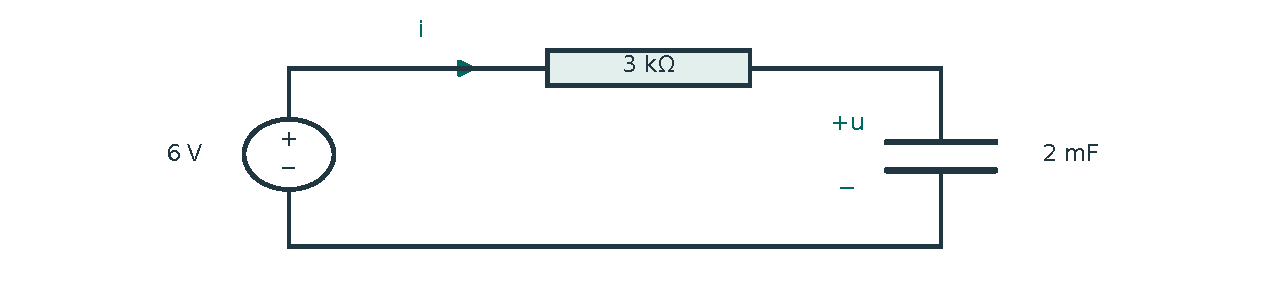
\includegraphics[width=.88\linewidth,height=49mm,keepaspectratio]{masche.pdf}\par}\capline{Die Maschengleichung hält die elektrischen Größen am selben Zeitpunkt zusammen.}
\seite{}{DAEs und Bindungen}\anchorpage{2}{abs4-1}{4.1 · Vom physikalischen Zwang zur Gleichung}\ey{ABSCHNITT 4.1}\ptitle{Vom physikalischen Zwang zur Gleichung}
\hypertarget{punkt4-1-1}{}\subt{4.1.1\enspace Mehrkörpermechanik und Kirchhoffsche Netze}
Der Faden zieht in radialer Richtung. Seine Spannung ist eine unbekannte Reaktion, die die vorgeschriebene Länge durchsetzt. Im elektrischen Knoten erzwingt die Ladungsbilanz eine Beziehung zwischen Zweigströmen. In beiden Fällen legt ein Gesetz Werte zur selben Zeit fest. Versucht man jede Größe ungeprüft vorwärts zu integrieren, gehen solche Beziehungen verloren.
\hypertarget{punkt4-1-2}{}\subt{4.1.2\enspace Semi-explizite und voll implizite Form}
In \(x'=f(t,x,z),\ 0=g(t,x,z)\) trägt \(x\) die Speicher, \(z\) die algebraischen Unbekannten. Die allgemeine Form \(F(t,y,y')=0\) nimmt auch gekoppelte Ableitungen auf. Beim RC-Kreis ist \(C U_C'-i=0\) die Speicherbilanz und \(U_C+Ri-U_s=0\) die algebraische Masche. Aus \(U_C(0)\) und \(U_s(0)\) folgt für \(R>0\) unmittelbar der zulässige Startstrom.
\seite{Rechenbeispiel}{DAEs und Bindungen}\anchorpage{2}{kap5}{Wer legt den Anfangsstrom fest?}\ptitle{Wer legt den Anfangsstrom fest?}


\lernziel{Sie können an einem Stromkreis entscheiden, welcher Anfangswert frei ist, die Bindung einsetzen und dieselbe Bewegung als DAE und als ODE berechnen.}
Zwei Personen stellen am Prüfplatz Anfangswerte ein. Eine wählt \(3\unitm V\) am Kondensator, die andere wünscht \(2\unitm{mA}\) Strom. In Reihe liegen eine ideale \(6\unitm V\)-Quelle, ein \(3\,\mathrm{k}\Omega\)-Widerstand und der Kondensator. Können beide Wünsche gleichzeitig gelten?
\minifig{masche}{32mm}{Der Strompfeil läuft vom positiven Quellenpol zum Kondensator. Mit diesen Vorzeichen addieren sich Widerstands- und Kondensatorspannung zur Quellenspannung.}
\subt{Die Rechnung vor jedem Zeitschritt}
Bei \(u=3\unitm V\) verbleiben am Widerstand \(6-3=3\unitm V\). Also gilt \(i=3/3000\unitm A=1\unitm{mA}\). Der gewünschte Strom von \(2\unitm{mA}\) würde am Widerstand bereits \(6\unitm V\) benötigen. Zusammen mit dem Kondensator wären das \(9\unitm V\).

Für \(C=2\unitm{mF}\) gilt jetzt \(C\dot u=i\), also \(\dot u=0{,}5\unitm{V/s}\). Das Speichergesetz bewegt die Spannung durch die Zeit. Die Maschengleichung \(0=6-u-3000i\) legt für jede momentane Spannung den Strom fest. Zusammen bilden beide Gleichungen eine differential-algebraische Gleichung, kurz DAE.
\notebox{Wechseln Sie die Sicht}{Setzen Sie \(i=(6-u)/3000\) in das Speichergesetz ein. Es bleibt \(\dot u=(6-u)/6\) für die Zahlenwerte in Volt und Sekunden. Bei \(u=3\) kommt dieselbe Steigung heraus. In einem Netz mit vielen Zweigen kann es leichter sein, die einzelnen Maschengleichungen stehen zu lassen.}

\srcs{\textbf{Kernweg}\enspace\see{rcvergleich}{Zwei Wege zum RC-Schritt}\quad\textbf{Vertiefung}\enspace\see{pendel}{Index des Pendels}\quad\see{ueb5}{Selbst prüfen}.}

\lektion{Eine Masche, zwei Rechenwege, derselbe Zeitschritt}{rcvergleich}{Kernweg}{DAE und Bindungen}
Rechnen Sie den ersten Schritt für einen zweiten Prüfplatz zweimal. Hier gelten \(U=5\unitm V,\ R=2000\,\Omega,\ C=0{,}001\unitm F\), zu Beginn ist der Kondensator ungeladen. Zuerst beseitigen wir den Strom in der Modellgleichung. Dann lassen wir Strom und Spannung als Unbekannte im Zeitschritt stehen. Was sollte sich an der Spannung ändern?
\subt{Weg 1 · Strom vorab eliminieren}
Aus \(i=(U-u)/R\) folgt \(\dot u=(U-u)/(RC)\). Bei \(h=0{,}5\unitm s\) ist \(h/(RC)=1/4\). Für Rückwärts Euler ergibt sich deshalb \(u_{k+1}=(u_k+1{,}25)/1{,}25\). Ein kalter Start \(u_0=0\) liefert zuerst \(1\unitm V\), im zweiten Schritt \(1{,}8\unitm V\).
\subt{Weg 2 · Spannung und Strom simultan bestimmen}
Aus \(C(u_{k+1}-u_k)/h=i_{k+1}\) und \(u_{k+1}+R i_{k+1}=U\) folgt pro Schritt
\[
 \begin{pmatrix}C/h&-1\\1&R\end{pmatrix}
 \binom{u_{k+1}}{i_{k+1}}=\binom{C u_k/h}{U}.
\]
Elimination der zweiten Unbekannten in dieser Matrix ergibt exakt die Rekursion von Weg 1. Umgekehrt rekonstruiert jede Spannung der Rekursion den einzigen passenden Strom. Damit stimmen beide Diskretisierungen für alle \(h>0\) bei identischem Start und exakt gelöstem linearen System überein.
{\tblstart\begin{tabularx}{\linewidth}{@{}rYYY@{}}\toprule
\hd{\(t\) [s]}&\hd{\(u\), beide Wege [V]}&\hd{\(i\) [mA]}&\hd{\(u\) exakt [V]}\\\midrule
0,0 &0,000&2,500&0,0000\\
0,5 &1,000&2,000&1,1060\\
1,0 &1,800&1,600&1,9673\\
2,0 &2,952&1,024&3,1606\\\bottomrule\end{tabularx}\par}
\notebox{Was bleibt zu messen?}{Nach zwei Sekunden beträgt der Fehler beider Rechnungen etwa \(0{,}2086\unitm V\). Das bestätigt zugleich die Gleichwertigkeit der beiden Wege und die endliche Zeitgenauigkeit. Halbieren Sie \(h\), um beides erneut und unabhängig voneinander zu prüfen.}
\srcs{Eigenes Zahlenexperiment \texttt{python labor.py rc}.}

\lektion{Eine Nebenbedingung im ersten Zeitschritt lösen}{dae}{Kernweg}{DAE und Bindungen}
\vorhersage{5}{Ein leerer Kondensator liegt über \(2000\,\Omega\) an \(5\unitm V\). Welchen Anfangsstrom erlaubt das Modell?}{kontrolleA}
Im Stromkreis trennte uns das Speichergesetz von der augenblicklichen Maschenbedingung. Beim Metallstab funktioniert derselbe Gedanke. Wir behalten den Temperaturüberschuss \(\theta_s\) im Kontakt und den abfließenden Wärmestrom \(q\) als eigene Unbekannte. Der Stab speichert Energie bei Temperaturüberschuss \(\theta\). Die drei Gesetze lauten
\[
 C\dot\theta=P-q,\qquad 0=\theta-\theta_s-R_1q,\qquad
 0=\theta_s-R_2q .
\]
Nur die erste Gleichung enthält eine Ableitung. In der Form \(M\dot y=f(t,y)\) ist \(M=\operatorname{diag}(C,0,0)\) für \(y=(\theta,\theta_s,q)\) singulär. Zu \(\theta(0)=0\) gehören \(\theta_s(0)=q(0)=0\). Nach dem Einschalten gilt \(\dot\theta(0^+)=10/120\unitm{K/s}\).
\subt{Rückwärts Euler in Residualform}
Wir ersetzen \(\dot\theta\) durch \((\theta_1-\theta_0)/h\) und erzwingen beide Kontaktgesetze am neuen Zeitpunkt. Bei \(h=60\unitm s\) lautet das lineare System in den zugehörigen SI-Einheiten
\[
 \begin{bmatrix}2&0&1\\1&-1&-1\\0&1&-3\end{bmatrix}
 \begin{bmatrix}\theta_1\\\theta_{s,1}\\q_1\end{bmatrix}
 =\begin{bmatrix}10\\0\\0\end{bmatrix}.
\]
Die unterste Zeile liefert \(\theta_{s,1}=3q_1\), die mittlere \(\theta_1=4q_1\). Oben bleibt \(9q_1=10\). Damit sind \(q_1=1{,}11111\unitm W\), \(\theta_{s,1}=3{,}33333\unitm K\) und \(\theta_1=4{,}44444\unitm K\).
\subt{Zwei voneinander unabhängige Kontrollen}
Das Leistungsresiduum \(C(\theta_1-\theta_0)/h-P+q_1\) verschwindet ebenso wie die beiden Temperaturresiduen. Gegen die analytische Transiente aus Kapitel 1 fehlt nach einer Minute trotzdem \(0{,}25568\unitm K\). Die algebraische Verträglichkeit und die zeitliche Genauigkeit beantworten verschiedene Fragen.
\notebox{Wann lohnt die DAE?}{In einem einzelnen linearen Kontakt ist die Elimination von Hand günstig. In einem Netz aus vielen Bauteilen lassen sich lokale Bilanzen und Koppelgesetze oft einfacher und überprüfbarer direkt als Residuen zusammensetzen.}
\srcs{Lineares Residualsystem zusätzlich mit \texttt{numpy.linalg.solve} nachgerechnet, \texttt{waermespeicher}.}

\seite{}{DAEs und Bindungen}\anchorpage{2}{abs4-2}{4.2 · Index und konsistente Bewegung}\ey{ABSCHNITT 4.2}\ptitle{Index und konsistente Bewegung}
\hypertarget{punkt4-2-1}{}\subt{4.2.1\enspace Differentiationsindex und Störungsempfindlichkeit}
Eine Bindung kann Ableitungen verbergen. Der Differentiationsindex zählt in der üblichen lokalen Konvention die benötigten Ableitungen der Gleichungen bis zu einer expliziten Bestimmung der Ableitungen aller Variablen. Für eine reguläre semi-explizite Bindung mit invertierbarem \(g_z\) erhält man \(z'=-g_z^{-1}(g_t+g_x f)\) nach einmaligem Differenzieren. Der Perturbationsindex fragt dagegen, bis zu welcher Ableitung eine Störung in Abschätzungen eingeht. Für allgemeine DAEs bedürfen beide Aussagen eigener Regularitätsannahmen.
\hypertarget{punkt4-2-2}{}\subt{4.2.2\enspace Das kartesische Pendel als Index-3-System}
Für \(r'=v,\ m v'=F-\lambda r\) bei konstanter Länge \(\ell>0\) gilt \(r\cdot r=\ell^2\). Einmal ableiten ergibt \(r\cdot v=0\). Noch einmal liefert \(v\cdot v+r\cdot(F-\lambda r)/m=0\), also \(\lambda=(m\,v\cdot v+r\cdot F)/\ell^2\). Zwei Ableitungen bestimmen die Kraft, die dritte liefert bei glattem \(F\) ihre Ableitung.
\hypertarget{punkt4-2-3}{}\subt{4.2.3\enspace Index eins, zwei und drei im Vergleich}
Die Positionsbindung ergibt Index drei, ihre Geschwindigkeitsform typischerweise Index zwei, die reguläre Beschleunigungsform mit eindeutig bestimmbarem Multiplikator Index eins. Wer nur die letzte Form integriert, muss Ort und Geschwindigkeit anfangs konsistent wählen. Eine kleine dauernde Verletzung des Geschwindigkeitszwangs summiert sich sonst im Ort auf.
\lektion{Index eins und konsistente Anfangswerte}{indexeins}{Vertiefung}{DAE und Bindungen}
Für \(\dot x=f(t,x,z),\ 0=g(t,x,z)\) sind \(x\) Differentialvariablen, \(z\) algebraische Unbekannte. Ist \(g\) stetig differenzierbar und \(g_z\) am konsistenten Startpunkt invertierbar, liefert der Satz über implizite Funktionen lokal \(z=\varphi(t,x)\). Nach Einsetzen liegt eine ODE für \(x\) vor. Einmaliges Ableiten der Nebenbedingung ergibt explizit
\[
 \dot z=-g_z^{-1}(g_t+g_x f).
\]
Das ist der reguläre semi-explizite Fall mit Differentiationsindex 1. Numerisch löst man das lineare System mit \(g_z\). Ein explizites Bilden seiner Inversen ist entbehrlich. Bei einem nahezu singulären \(g_z\) kann die Reduktion empfindlich werden.
\subt{Eine Masche als Kontrollrechnung}
Eine \(5\unitm V\)-Quelle lädt einen ungeladenen Kondensator \(C_e=1\unitm{mF}\) über \(R_e=2\,\mathrm{k}\symup{\Omega}\). Nach Kirchhoff und dem Kondensatorgesetz gilt \(C_e\dot u=i,\ 0=5-u-R_ei\). Zu \(u(0)=0\) gehört \(i(0)=2{,}5\unitm{mA}\), also \(\dot u(0)=2{,}5\unitm{V/s}\). Ein vorgegebener Startstrom von \(1\unitm{mA}\) ließe ein Spannungsresiduum von \(3\unitm V\).

Elimination liefert \(u(t)=5(1-e^{-t/2})\unitm V\) und \(i(t)=2{,}5e^{-t/2}\unitm{mA}\), für \(t\) in Sekunden. So lassen sich Strom, Spannung und Maschenresiduum unabhängig prüfen.
\minifig{rc}{24mm}{Jeder zulässige Zustand des RC-Kreises liegt auf der Maschengeraden. Die Anfangsspannung legt ihren Startpunkt fest. Die Speicherbilanz bestimmt, wie schnell der Zustand auf der Geraden wandert.}
\subt{Was ein Residualsolver benötigt}
In der Form \(F(t,y,\dot y)=0\) setzt ein BDF-Schritt \(\dot y_{n+1}\approx a_0y_{n+1}+b\) ein. Newton verwendet dann \(F_y+a_0F_{\dot y}\). IDA kann für geeignete Index-1-Probleme konsistente algebraische Startwerte und Differentialableitungen aus einer Startschätzung ermitteln. Die jeweils freigegebenen Unbekannten müssen zum physikalischen Anfangszustand passen. Unterschiedliche Residualeinheiten erhalten eigene Bezugsgrößen.
\task{5}{Berechnen Sie den Zeitpunkt, zu dem der Kondensator \(2{,}5\unitm V\) erreicht, und den zugehörigen Strom. Welche falsche Kurve könnte die Maschengleichung dennoch zu jeder Zeit erfüllen?}
\srcs{\refbk{ida}{SUNDIALS IDA, Anfangswerte und nichtlinearer Schritt} · \see{diode}{C21-Diode in Residualform}.}

\lektion{Ist eine DAE eine besonders steife ODE?}{grenzfall}{Vertiefung}{DAE und Bindungen}
Ein träger Sensor folgt einer Größe \(x\) mit dem Messwert \(z\). In dimensionslosen Einheiten untersuchen wir das Modell
\[
 \dot x=-z,\qquad \varepsilon\dot z=x-z,\qquad \varepsilon>0.
\]
Je kleiner die positive Sensorzeit \(\varepsilon\), desto schneller folgt \(z\) dem Eingang. Für jedes positive \(\varepsilon\) ist das eine ODE in zwei Zuständen. Wir dürfen \(x(0)\) und \(z(0)\) getrennt festlegen. Formales Setzen von \(\varepsilon=0\) ergibt \(\dot x=-z,\ 0=x-z\). Jetzt müssen beide Startwerte gleich sein. Damit ist die Zahl freier Anfangsdaten gesunken.
\subt{Die schnelle Zeitskala ausrechnen}
Einsetzen von \(z=-\dot x\) ergibt \(\varepsilon\ddot x+\dot x+x=0\). Die beiden Exponenten lauten
\[
 \lambda_{\pm}=\frac{-1\pm\sqrt{1-4\varepsilon}}{2\varepsilon}.
\]
Für kleine positive \(\varepsilon\) (hier \(\varepsilon<1/4\)) ergibt Rationalisieren \(\lambda_+=-2/(1+\sqrt{1-4\varepsilon})\to-1\). Aus \(\lambda_++\lambda_-=-1/\varepsilon\) folgt \(\lambda_-\sim-1/\varepsilon\). Die schnelle Mode kann eine unverträgliche Sensorauslenkung in einer kurzen \emph{Anfangsschicht} abbauen.
\subt{Was geschieht beim Start?}
Wähle \(x(0)=1,\ z(0)=0\). Die ODE hat anfangs \(\dot x=0\), \(\dot z=1/\varepsilon\). Die DAE erzwingt zu \(x(0)=1\) den Start \(z(0)=1\) und \(\dot x=-1\). Für die Sensorgröße kann es mit diesen Daten keine gleichmäßige Konvergenz auf einem Intervall \([0,T]\) geben. Schon bei \(t=0\) beträgt ihre Abweichung immer eins. Gleichmäßige Konvergenz würde verlangen, dass der größte Fehler auf dem ganzen Intervall gegen null geht.
\notebox{Zwei verschiedene Operationen}{Die Ordnungsreduktion aus Kapitel 1 ist eine exakte Umbenennung der Unbekannten. Der Grenzübergang \(\varepsilon\to0\) entfernt eine Zeitskala und verändert zulässige Anfangsdaten. Eine DAE kann so entstehen. Andere DAEs folgen unmittelbar aus idealen Zwangs- oder Koppelgesetzen.}
\srcs{\refbk{stiff}{Hairer und Wanner, steife Probleme und singuläre Störungen}.}

\lektion{Eine geometrische Bindung führt zu höherem Index}{pendel}{Vertiefung}{DAE und Bindungen}
Ein Massenpunkt \(m\) hängt an einem starren, masselosen Stab der Länge \(\ell\). Das Lager ist fest und reibungsfrei. Mit Ortsvektor \(r=(x,y)\), Geschwindigkeit \(v\), Schwerebeschleunigung \(\mathbf g=(0,-g)\) und Zwangskraft \(-\lambda r\) gilt
\[
 \dot r=v,\qquad m\dot v=m\mathbf g-\lambda r,\qquad
 0=r^\mathsf T r-\ell^2.
\]
Die Bindung selbst enthält den Multiplikator \(\lambda\) nicht. Deshalb greift die einfache Elimination über \(g_z\) hier nicht.
\subt{Die verborgenen Bedingungen ableiten}
Einmaliges Ableiten des Längenquadrats ergibt \(r^\mathsf T v=0\). Der Start erfordert eine tangentiale Geschwindigkeit. Erneutes Ableiten liefert \(v^\mathsf T v+r^\mathsf T\dot v=0\). Zusammen mit der Bewegungsgleichung ergibt sich auf der Bindungsfläche
\[
 \lambda=\frac{m}{\ell^2}\big(v^\mathsf Tv+r^\mathsf T\mathbf g\big).
\]
Zwei Ableitungen bestimmen also die Zwangskraft. Für eine explizite Gleichung auch für \(\dot\lambda\) ist eine weitere Ableitung nötig. Die kartesische Form mit Positionsbindung hat den klassischen Differentiationsindex 3.

Für \(m=1\unitm{kg},\ \ell=1\unitm m,\ r=(0,-1)\unitm m,\ v=(2,0)\unitm{m/s}\) ist die Stabkraft \(\lambda\ell=13{,}81\unitm N\) nach oben. Gewicht und benötigte Zentripetalkraft addieren sich im Betrag. Dieser Start prüft Vorzeichen und Einheiten.
\subt{Welche Formulierung passt?}
Mit \(r=\ell(\sin\varphi,-\cos\varphi)\) erfüllt jede Winkeltrajektorie die Länge und es folgt \(\ddot\varphi=-(g/\ell)\sin\varphi\). Für das ebene Einzelpendel ist eine ODE in Winkelkoordinaten besonders einfach. Für gekoppelte Mechanismen sind Zwangsformulierungen oft bequemer. Dann kommen Indexreduktion und Projektion oder RATTLE mit Positions- und Geschwindigkeitsbindung infrage. Prüfen Sie Positionsfehler \(r^\mathsf T r-\ell^2\), Tangentialitätsfehler \(r^\mathsf T v\) und die Energie getrennt. Eine Integration nur auf Beschleunigungsebene kann in der Position driften.
\srcs{\refbk{stiff}{Hairer und Wanner, Differential-algebraic equations} · \refbk{geom}{Geometrische Integration}.}

\seite{}{DAEs und Bindungen}\anchorpage{2}{abs4-3}{4.3 · Indexreduktion, Drift und Projektion}\ey{ABSCHNITT 4.3}\ptitle{Indexreduktion, Drift und Projektion}
\hypertarget{punkt4-3-1}{}\subt{4.3.1\enspace Warum die Länge langsam wandert}
Die zweimal abgeleitete Bedingung \(g''=0\) lässt \(g(t)=a+bt\) zu. Ein kleiner Fehler im Anfangswert \(b\) erzeugt selbst bei exakt verschwindendem Beschleunigungsdefekt eine linear anwachsende Längenverletzung. Protokollieren Sie bei jedem Schritt sowohl \(r\cdot r-\ell^2\) als auch \(r\cdot v\).
\hypertarget{punkt4-3-2}{}\subt{4.3.2\enspace Baumgarte-Stabilisierung}
Ersetzt man die Beschleunigungsbedingung durch \(g''+2\alpha g'+\beta^2g=0\), dämpfen positive Parameter einen Bindungsfehler. Bei \(\alpha=\beta\) besitzt das Fehlerpolynom die doppelte Wurzel \(-\alpha\). Sehr große Werte verkürzen die künstliche Zeitkonstante und können ihrerseits die Schrittweite begrenzen. Die Koeffizienten tragen die Einheit \(\mathrm{s}^{-1}\).
\hypertarget{punkt4-3-3}{}\subt{4.3.3\enspace SHAKE, RATTLE und eine einfache Gegenprobe}
Für festen Radius bringt \(r\leftarrow\ell r/\|r\|\) den Ort zurück auf den Kreis. Danach entfernt \(v\leftarrow v-r(r\cdot v)/\ell^2\) den radialen Geschwindigkeitsanteil. Diese einfache Kontrolle erklärt die beiden Defekte. SHAKE und RATTLE bestimmen ihre Korrekturen innerhalb eines konsistenten Zwangsschritts mit Multiplikatoren. Die symplektische Eigenschaft gilt unter den üblichen glatten Hamilton-Annahmen und ausreichend genau gelösten Zwangsgleichungen. Die zwei Kontrollen für das Stiftpendel stehen bei \see{befundrattle}{C07}.

Bei RATTLE für ein separables mechanisches System mit konstanter positiver Massenmatrix \(M\) und regulärer holonomer Bindung \(g(q)=0\) geht der erste Impuls von der alten Lage aus. Man wählt seinen Multiplikator so, dass die mit dem Halbzeitimpuls fortgeschriebene Lage \(q_{n+1}=q_n+hM^{-1}p_{n+1/2}\) die Gleichung \(g(q_{n+1})=0\) erfüllt. In der zweiten Impulshälfte wirkt die Zwangskraft in der Normalenrichtung der neuen Lage. Ihr Multiplikator erzwingt \(g_q(q_{n+1})M^{-1}p_{n+1}=0\). Ein Protokoll mit beiden Defekten deckt auch den Fall auf, dass die Länge stimmt, der Impuls aber noch aus der Tangentialebene zeigt.
\seite{}{DAEs und Bindungen}\anchorpage{2}{abs4-4}{4.4 · Direkte DAE-Integration}\ey{ABSCHNITT 4.4}\ptitle{Direkte DAE-Integration}
\hypertarget{punkt4-4-1}{}\subt{4.4.1\enspace Radau IIA an regulären Bindungen}
Ein Kollokationsschritt sucht Stufenableitungen \(K_i\) mit \(F(t_n+c_i h,Y_i,K_i)=0\) und \(Y_i=y_n+h\sum_j a_{ij}K_j\). Die letzte Stufe liefert den Endzustand. Beim Index eins sichert eine lokal eindeutig lösbare algebraische Gleichung den Ast. Bei Hessenberg-DAEs vom Index zwei sind weitere Rangbedingungen und konsistente Startwerte nötig. Die Fehlerordnung kann für algebraische Größen geringer ausfallen. Kritisch wird ein Schritt, wenn die erforderliche Matrix am Ast singulär wird.
\hypertarget{punkt4-4-2}{}\subt{4.4.2\enspace Der Vertrag von IDA und IDAS}
Für einen BDF-Schritt lässt sich \(y'=\gamma y+d\) schreiben. Das Newton-System verwendet daher \(F_y+\gamma F_{y'}\). Der Nutzer liefert die Residualfunktion, ein kompatibles Paar \((y_0,y'_0)\) oder die für eine unterstützte Initialisierung nötige Aufteilung und Schätzwerte. Die C21-Diode rechnet ein Index-1-Beispiel mit IDAS bis zur nächsten Umschaltung. Bei einem Astwechsel werden Startwerte und Historie neu aufgebaut.
\srcs{\href{https://sundials.readthedocs.io/en/latest/ida/Mathematics_link.html}{SUNDIALS, mathematischer Vertrag von IDA} · \see{diode}{C21-Residualvergleich}.}
\werkblatt{4}{Selbst prüfen}{ueb5}{Strom, Spannung und Bindung}

\merke{Die Bindung entscheidet, welche Momentanwerte zusammenpassen. Das Speichergesetz und der Zeitschritt entscheiden, wie weit der Zustand bis zur nächsten Zeit wandert.}
\subt{A · Dieselbe Schaltung auf zwei Wegen}
Eine ideale \(8\unitm V\)-Quelle, \(R=2\,\mathrm{k}\Omega\) und \(C=1\unitm{mF}\) liegen in Reihe. Zu Beginn gilt \(u_0=2\unitm V\). Bestimmen Sie \(i_0\) und \(\dot u_0\). Berechnen Sie einen Rückwärts-Euler-Schritt von \(0{,}5\unitm s\) einmal durch vorherige Elimination von \(i\) und einmal mit den beiden Gleichungen am Schrittende.
\subt{B · Startdaten auf Verträglichkeit prüfen}
Ein Messprotokoll meldet für dieselbe Quelle zur gleichen Zeit \(u=3\unitm V,\ i=1\unitm{mA}\). Setzen Sie beide Werte in \(r=8-u-Ri\) ein. Darf das ideale Modell exakt mit diesem Wertepaar starten? Wenn Sie der Spannungsmessung vertrauen, welchen Strom brauchen Sie?
\subt{C · Eine nichtlineare Bindung ableiten}
In einem dimensionslosen Modell gilt \(\dot x=-z,\quad z=x^2\). Für \(x_0=2\) bestimmen Sie \(z_0,\dot x_0,\dot z_0\). Bauen Sie eine eigenständige Kontrolle, indem Sie für \(t\ge0\) den Vorschlag \(x(t)=2/(1+2t)\) und \(z(t)=x(t)^2\) in die ursprünglichen Gleichungen einsetzen.
\hilfe{Bei Rückwärts Euler stehen \(i_1\) und \(u_1\) auf der rechten Seite. In C ist \(z\) als Funktion von \(x(t)\) zu lesen.}

\schreibfeld

\srcs{\see{loesweg5}{Lösungswege A, B und C}\quad·\quad\see{kap5}{Zum Kapitelauftakt}.}

\werkblatt{4}{Lösungswege}{loesweg5}{Strom, Spannung und Bindung}

\subt{A · Elimination und gemeinsame Lösung}
Aus \(8-u_0=Ri_0\) folgen \(i_0=3\unitm{mA}\) und \(\dot u_0=i_0/C=3\unitm{V/s}\). Mit \(RC=2\unitm s\) lautet die reduzierte Gleichung \(\dot u=(8-u)/2\). Rückwärts Euler gibt \(u_1=2+0{,}25(8-u_1)\), also \(1{,}25u_1=4\) und \(u_1=3{,}2\unitm V\).

Für die gekoppelte Form gilt \(i_1=C(u_1-2)/h=0{,}002(u_1-2)\) in Ampere. Die Maschengleichung wird \(u_1+2000\cdot0{,}002(u_1-2)=8\). Das liefert \(5u_1=16\), denselben Spannungswert und \(i_1=2{,}4\unitm{mA}\). Am Schrittende sinkt der Strom wie beim Laden zu erwarten.
\subt{B · Einen Widerspruch in Volt ausdrücken}
Der Rest ist \(8-3-2000\cdot0{,}001=3\unitm V\). Diese Startdaten können die ideale Maschengleichung nicht erfüllen. Wird \(3\unitm V\) beibehalten, folgt \(i=(8-3)/2000=2{,}5\unitm{mA}\). Welche Messung am realen Prüfstand vertrauenswürdiger ist, müsste eigens geklärt werden.
\subt{C · Eine abhängige Steigung rekonstruieren}
Für \(x_0=2\) ist \(z_0=4\) und \(\dot x_0=-4\). Differenzieren der Bindung liefert \(\dot z=2x\dot x\), am Start also \(-16\). Für den Lösungsvorschlag gilt \(\dot x=-4/(1+2t)^2=-x^2=-z\). Die zweite Gleichung gilt wegen \(z=x^2\) ebenfalls. Der Vorschlag trifft den konsistenten Start und erfüllt beide ursprünglichen Gleichungen für \(t\ge0\).
\notebox{Ein schneller Gegencheck}{Ein kleines algebraisches Residuum besagt nur, dass die Komponenten zusammenpassen. Auch eine falsche Zeitkurve \(u(t)\) kann zusammen mit \(i(t)=(8-u(t))/R\) jederzeit die Masche erfüllen.}

\srcs{\see{ueb5}{Noch einmal selbst rechnen}\quad·\quad\see{schluss5}{Forschungsstand und Beweisfragen}.}

\kapschluss{4}{Index, Anfangsdaten und Lösungszweig}{schluss5}
\subt{Stand der Forschung}
Kunkel und Mehrmann systematisieren die verschiedenen Regularitäts- und Indexbegriffe. Bolten und Wimmer analysieren 2026 eine spektrale Deferred-Correction-Methode für semi-explizite DAEs vom Index eins. Sie korrigieren Näherungen an mehreren Zeitknoten und erzwingen bei jeder Iteration die algebraischen Bindungen. Die untersuchte Problemklasse und ihre Regularität sind wesentliche Voraussetzungen für die Konvergenzaussage.
\subt{Was ist bewiesen?}
Bei \(g(t,x,z)=0\) und invertierbarem \(g_z\) existiert lokal ein stetig differenzierbarer Ast \(z=\varphi(t,x)\) unter den Voraussetzungen auf S.\,\pagelink{indexeins}. Ist \(g\) von Klasse \(C^k\), so ist der Ast von Klasse \(C^k\). Bei \(g=z-x|x|\) ist \(g_z=1\), doch \(\varphi=x|x|\) ist in null nur einmal differenzierbar, denn \(\varphi^{\prime}=2|x|\). Einsetzen dieses Asts ergibt eine kleinere ODE. Beim linearen RC-Kreis ergab eine direkte Elimination sogar identische Rückwärts-Euler-Schritte. Für das Pendel zeigt die abgeleitete Bedingung \(r^\mathsf Tv=0\), warum eine korrekte Länge allein noch keine zulässige Anfangsgeschwindigkeit garantiert.
\subt{Ergebnis der Nachuntersuchung}
Die Niedrigstromlösung der C21-Diode lässt sich für die Schaltungsparameter des Versuchs auf beiden Seiten der Schaltfläche fortsetzen. Der Nachweis beruht auf einer zeitlich gleichmäßigen Spannungsgrenze und einer unteren Schranke für die algebraische Ableitung.
\notebox{Beim Lesen von Indexangaben}{Fragen Sie nach dem Indexbegriff, der Formulierung und dem betrachteten Gebiet. Dieselbe Bewegung hat im Winkelmodell eine ODE und in kartesischen Ortskoordinaten eine höherindizierte DAE.}
\srcs{\see{befunddiode}{Nachweis und Ergebnis} · \href{https://doi.org/10.4171/ETB/28}{Kunkel und Mehrmann (2024), Differential-Algebraic Equations} · \href{https://doi.org/10.1007/s10915-026-03385-7}{Bolten und Wimmer (2026), Spectral Deferred Corrections for DAEs of Index One}.}
\lektion{Welche Matrix der Residualsolver wirklich löst}{pruefung4}{Herleitung und Gegenprobe}{Kapitel 4}
Am RC-Kreis stellen wir \(R=3000\,\Omega\), \(C=0{,}002\unitm F\) und \(U_s=6\unitm V\) ein. Zu Beginn sei \(u_0=3\unitm V\). Die Masche verlangt \(i_0=(6-3)/3000=1\unitm{mA}\). Wie zwingt ein Zeitschritt die künftige Spannung und den künftigen Strom wieder auf dieselbe Masche?

Wir ordnen die Unbekannten als \(y=(u,i)\) und verwenden die Residuen \(F_1=C\dot u-i\), \(F_2=u+Ri-U_s\). Bei rückwärts Euler ist \(\dot u_1=(u_1-u_0)/h\). Eine Korrektur \(\delta u\) ändert gleichzeitig diesen Differenzenquotienten um \(\delta u/h\). Die Kettenregel liefert für das Newton-System
\[
 F_y+h^{-1}F_{\dot y}=
 \begin{pmatrix}C/h&-1\\1&R\end{pmatrix}.
\]
In der ersten Zeile wird in Ampere, in der zweiten in Volt bilanziert. Für \(h=1\unitm s\) gilt \(i_1=0{,}002(u_1-3)\) bei Zahlenwerten in SI-Einheiten. Setzen wir das in \(u_1+3000i_1=6\) ein, folgt \(7u_1=24\). Daher sind \(u_1=24/7\unitm V\) und \(i_1=6/7\unitm{mA}\). Einsetzen in beide Originalzeilen ergibt null. Das lineare Modell benötigt bei exakter Arithmetik nur eine Newton-Korrektur mit dieser Matrix.

Für eine BDF ersetzt der Koeffizient der aktuellen Unbekannten im Ableitungsansatz den Faktor \(1/h\). Genau diesen Koeffizienten muss die Jacobi-Routine des Residualsolvers berücksichtigen. Die Matrix ist hier wegen \(1+RC/h>0\) für \(h>0\) regulär.
\notebox{Achtung, Falle}{Ein gemeinsames absolutes Abbruchkriterium für Zahlenwerte in Ampere und Volt verändert seine Bedeutung beim Wechsel zu Milliampere. Skalieren Sie die beiden Gleichungen mit benannten Bezugsgrößen und kontrollieren Sie die physikalischen Residuen zusätzlich in Originaleinheiten.}
\srcs{\see{abs4-4}{IDA und konsistente Anfangsdaten} · \see{alg4}{Bindung vor und nach einem Schritt}.}

\lektion{Zwei Gegenproben für einen Bindungsschritt}{alg4}{Werkstatt}{Kapitel 4}
Ein Programm meldet eine exakte Fadenlänge. Im nächsten Schritt wächst sie dennoch wieder. Wie prüfen wir, ob bereits die Geschwindigkeit nach außen zeigt? Der Lehralgorithmus illustriert die Diagnose für einen Kreis mit festem Radius.
{\small\begin{verbatim}
ort = laenge * ort / norm(ort)
radial = dot(ort, tempo) / laenge**2
tempo = tempo - radial * ort
pruefe(dot(ort, ort) - laenge**2)
pruefe(dot(ort, tempo))
\end{verbatim}}
\subt{Selbst rechnen}
Ein normierter Pendelzustand hat r=(1,0) und \(v=(0{,}02;1)\). Was verändert die zweite Zeile der Projektion?
\notebox{Lösung}{Das Skalarprodukt ist 0,02. Abziehen der radialen Komponente ergibt v=(0,1). Der Betrag des Ortes war schon korrekt. Diese Projektion demonstriert den Tangentialtest. Für die Langzeitdynamik folgt der geprüfte RATTLE-Schritt im Pendelversuch.}

\seite{}{Hybride Systeme}\anchorpage{1}{neu5}{5 · Hybride Systeme, Diskontinuitäten und Ereignissteuerung}\ey{KAPITEL 5}\ptitle{Hybride Systeme, Diskontinuitäten und Ereignissteuerung}
Ein Ball fällt. Zwischen zwei gespeicherten Höhen ist er kurz auf den Boden getroffen und bereits wieder aufgestiegen. Ein Modell, das erst am nächsten Ausgabetakt reagiert, kann Energie gewinnen oder den Stoß ganz übersehen. Wie findet man den Augenblick, in dem das Bewegungsgesetz wechselt?
\subt{Der Weg durch das Kapitel}
{\tblstart\begin{tabularx}{\linewidth}{@{}Yr@{}}\toprule
\hyperlink{abs5-1}{5.1 · Zeit- und Zustandsereignisse} & \pagelink{abs5-1}\\[2pt]
\hyperlink{abs5-2}{5.2 · Nullstellen während eines Schritts} & \pagelink{abs5-2}\\[2pt]
\hyperlink{abs5-3}{5.3 · Reset und Neustart} & \pagelink{abs5-3}\\[2pt]
\hyperlink{abs5-4}{5.4 · Chattering und Zeno-Folgen} & \pagelink{abs5-4}\\[2pt]
\bottomrule\end{tabularx}\par}
\par\vfill{\centering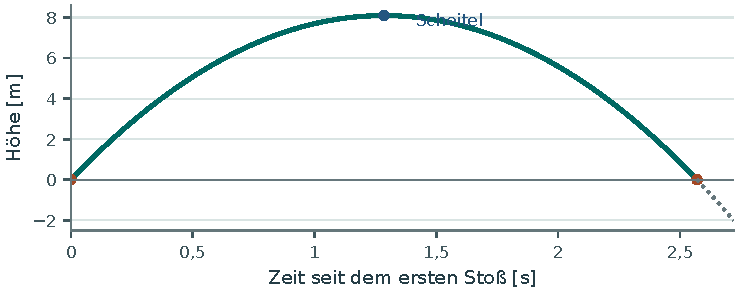
\includegraphics[width=.88\linewidth,height=49mm,keepaspectratio]{ball.pdf}\par}\capline{Jeder glatte Flug endet am gerichteten Kontakt.}
\seite{}{Hybride Systeme}\anchorpage{2}{abs5-1}{5.1 · Zeit- und Zustandsereignisse}\ey{ABSCHNITT 5.1}\ptitle{Zeit- und Zustandsereignisse}
\hypertarget{punkt5-1-1}{}\subt{5.1.1\enspace Welcher Zeitpunkt ist im Voraus bekannt?}
Ein Steuergerät tastet alle zehn Millisekunden ab. Der nächste Takt liegt vor dem Integrationsschritt fest. Wann derselbe Antrieb seinen Anschlag erreicht, hängt von Ort und Geschwindigkeit ab. Planen Sie Kalenderereignisse direkt. Für Zustandsereignisse benötigt man zusätzlich eine Suchregel innerhalb des kontinuierlichen Fluges.
\hypertarget{punkt5-1-2}{}\subt{5.1.2\enspace Wächter, Richtung und Modus}
Ein Bodenwächter lautet \(g(t,y)=q\) mit zulässiger Lage \(q\ge0\). Ein Stoß ist nur für Annäherung, also \(v<0\), aktiv. Derselbe Nullwert unmittelbar nach dem Rückprall darf keinen zweiten Stoß auslösen. Die gerichtete Freigabe und der aktive Modus sind damit Teil des Modells.
\seite{Rechenbeispiel}{Hybride Systeme}\anchorpage{2}{kap7}{Kann eine Schaltung zwischen zwei Messungen verschwinden?}\ptitle{Kann eine Schaltung zwischen zwei Messungen verschwinden?}


\lernziel{Sie können einen Schaltzustand mitführen, eine Ereignisrichtung angeben und erklären, weshalb eine Abfrage nur an Schrittenden Übergänge verpassen kann.}
Eine Routine meldet „kein Ereignis“, weil ihr Signal bei Sekunde 0 und bei Sekunde 1 positiv ist. Sie dürfen einmal dazwischen messen. Zu welchem Zeitpunkt würden Sie messen, um die Meldung an der gezeichneten Kurve zu überprüfen?
\minifig{zweiwurzeln}{37mm}{Ein einziger großer Schritt tastet nur die beiden äußeren Punkte ab. Der zusätzliche Punkt bei einer halben Sekunde liegt auf der anderen Seite der Schwelle.}
\subt{Eine Meldung mit Papier und Bleistift prüfen}
Für den Zahlenwert \(s=t/(1\unitm s)\) sei das Signal \(g=(s-0{,}25)(s-0{,}75)\). An beiden Enden erhalten wir \(+0{,}1875\), in der Mitte \(-0{,}0625\). Wegen der Stetigkeit liegt in jeder Hälfte mindestens eine Nullstelle. Die Faktoren liefern sogar die genauen Zeiten \(0{,}25\) und \(0{,}75\unitm s\).

Soll das Gerät nur beim Eintritt in den negativen Bereich schalten, zählt die erste der beiden Nullstellen. Zur zweiten Zeit verlässt das Signal den Bereich. Ein Ereignis braucht daher auch eine Richtung und eine Regel für das, was anschließend geschieht.
\notebox{Jetzt Sie}{Welche zusätzliche Information braucht ein Thermostat bei genau \(20\,^\circ\mathrm C\), wenn er bei \(19\,^\circ\mathrm C\) einschaltet und bei \(21\,^\circ\mathrm C\) ausschaltet? Prüfen Sie je eine Vorgeschichte von oben und von unten. Der bisherige Schaltzustand entscheidet, ob der Raum jetzt heizt.}

\srcs{\textbf{Kernweg}\enspace\see{hybrid}{Thermostat}\quad\textbf{Vertiefung}\enspace\see{qfehler}{Fehler durch Quantisierung}\quad\see{ueb7}{Selbst prüfen}.}

\lektion{Ein Thermostat als erstes Ereignismodell}{hybrid}{Kernweg}{Hybride Systeme}
\vorhersage{7}{Eine Schaltfunktion ist an beiden Schrittenden positiv. Kann sie dazwischen zweimal das Vorzeichen wechseln?}{kontrolleB}
Bei \(20\,^\circ\mathrm C\) kann dieselbe Heizung gerade ein- oder ausgeschaltet sein. Wir nehmen im warmen Modus eine Rate von \(1\unitm{K/min}\) und im kühlen Modus \(-0{,}5\unitm{K/min}\) an. Bei \(19\,^\circ\mathrm C\) schaltet sie beim Absinken ein, bei \(21\,^\circ\mathrm C\) beim Ansteigen aus. Erst Temperatur und Schaltzustand zusammen reichen zur Vorhersage.
\subt{Fluss, Wächter, Richtung und Übergang}
Im Modus „an“ gilt \(\dot T=1\), im Modus „aus“ \(\dot T=-0{,}5\), mit Zeit in Minuten. Ein \emph{Wächter} ist eine Funktion, deren Nullstelle einen Übergang auslösen kann. Im Heizmodus suchen wir eine steigende Nullstelle von \(T-21\). Der Übergang setzt den Modus auf „aus“ und lässt \(T\) stetig. Im Kühlmodus suchen wir eine fallende Nullstelle von \(T-19\). Die obere und die untere Schwelle verhindern unmittelbares Hin- und Herschalten. Diesen Gedächtniseffekt nennt man Hysterese.

Start bei \(20\,^\circ\mathrm C\), Heizung an. Nach einer Minute sind \(21\,^\circ\mathrm C\) erreicht. Vier Minuten später sind es \(19\,^\circ\mathrm C\), zwei weitere Minuten später erneut \(21\,^\circ\mathrm C\). Startet der gleiche Raum bei derselben Temperatur mit ausgeschalteter Heizung, folgt der erste Übergang schon aus einem anderen Wächter. Die Temperatur allein beschreibt die Zukunft daher nicht vollständig.
\subt{Drei Uhren im Modell}
Ein fester Reglertakt ist vorab bekannt. Die physikalische Schaltzeit ergibt sich aus der aktuellen Bahn. Eine interne Zustandsmeldung eines QSS-Verfahrens entsteht, wenn ein numerisch festgelegter Schwellenabstand erreicht ist. Nur die ersten beiden Zeitarten gehören hier zur technischen Aufgabenstellung.
\notebox{Terminologie}{Der \emph{Reset} ist die Abbildung vom Zustand unmittelbar vor dem Übergang auf den Zustand unmittelbar danach. Er kann Größen unverändert lassen oder sprunghaft ändern. Beim \see{praxisdae}{C07-Stiftpendel am Drehpunktwechsel} springt die Winkelgeschwindigkeit. Aus \(\omega^-=-1\unitm{rad/s}\) wird \(\omega^+=-10/3\unitm{rad/s}\), während die Bahngeschwindigkeit bei \(-1\unitm{m/s}\) bleibt. Beim Kugelstoß springen die Bahngeschwindigkeiten.}

\seite{}{Hybride Systeme}\anchorpage{2}{abs5-2}{5.2 · Nullstellen während eines Schritts}\ey{ABSCHNITT 5.2}\ptitle{Nullstellen während eines Schritts}
\hypertarget{punkt5-2-1}{}\subt{5.2.1\enspace Ein Intervall einklammern}
Ist \(G(t)=g(t,p(t))\) für die dichte Bahn \(p\) stetig und haben die Endpunkte entgegengesetzte Vorzeichen, liegt mindestens eine Nullstelle dazwischen. Monotonie sichert höchstens eine. Ein Vorzeichenwechsel über einen Modussprung besitzt diese Aussagekraft erst nach Trennung der glatten Abschnitte.
\hypertarget{punkt5-2-2}{}\subt{5.2.2\enspace Bisektion, Regula falsi und Brent}
Bei Bisektion berechnet man die Mitte, wertet dort den Wächter aus und behält die Hälfte mit Wechsel. Nach \(k\) Halbierungen misst die Klammer \(h/2^k\). Regula falsi verwendet den Schnittpunkt der Sekante mit der Zeitachse. Brent kombiniert schnelle Interpolation mit einer abgesicherten Halbierung. Das Abbruchmaß ist die verbleibende Zeitbreite. Ist zusätzlich \(|G'|\ge m>0\) belegt, übersetzt sich ein Wächterfehler \(\varepsilon\) in höchstens \(\varepsilon/m\) Zeitfehler bei passend isolierter Wurzel.
\hypertarget{punkt5-2-3}{}\subt{5.2.3\enspace Zwei Durchgänge oder eine tangentiale Berührung}
Der Wächter \((t-1/4)(t-3/4)\) ist am Anfang und Ende von \([0,1]\) positiv. Er hat zwei Nullen. Der Wächter \((t-1/2)^2\) berührt die Null einmal. Beide Fälle entgehen dem bloßen Endpunkttest. Polynomextrema, Unterteilung oder ein physikalisch begründeter Höchstschritt können geeignete Klammern liefern. Eine endliche Stichprobe allein beweist deren Vollständigkeit nicht.
\lektion{Vertiefung · Eine glatte Lösung ohne Taylor-Darstellung}{flach}{Vertiefung}{Hybride Systeme}
Das Ventil der Einleitung hat einen sichtbaren Knick in der Volumenkurve erzeugt. Könnte man immer eine Potenzreihe verwenden, wenn stattdessen alle Ableitungen existieren? Ein von null anlaufender Zufluss beantwortet diese Frage. Zeit und Menge seien hier dimensionslos. Wir betrachten das Anfangswertproblem
\[
 x'(s)=q(s),\quad x(0)=0,\qquad
 q(s)=
 \begin{cases}
 0,&s\le0,\\
 \exp(-1/s^2),&s>0 .
 \end{cases}
\]
\subt{Was alle Ableitungen am Start ergeben}
Für \(s>0\) ist jede Ableitung von \(q\) ein Polynom in \(1/s\) mal \(\exp(-1/s^2)\). Dies folgt durch wiederholtes Ableiten. Alle diese Produkte gehen für \(s\downarrow0\) gegen null, denn \(r^m e^{-r^2}\to0\) für \(r\to\infty\) und jedes feste \(m\). Dasselbe gilt nach Division durch \(s\). Induktion mit dem Differenzenquotienten liefert deshalb \(q^{(j)}(0)=0\) für jede Ordnung \(j\). Von links ist die Funktion ohnehin null.
\subt{Eine Vorhersage und ihr Gegenbeweis}
Die eindeutige Lösung lautet \(x(s)=\int_0^s q(u)\dg u\). Damit verschwinden \(x(0)\) und alle Ableitungen von \(x\) am Start. Die Taylorreihe um null ist also die Nullreihe. Für jedes \(s>0\) integriert man jedoch eine positive Funktion über ein Intervall positiver Länge, folglich ist \(x(s)>0\). Die Reihe stimmt in keiner Umgebung von null mit der Lösung überein. Diese ODE hat eine eindeutige, beliebig oft differenzierbare Lösung und besitzt am Start keine reell-analytische Lösung.
\notebox{Was ein Zeitschritt hier anders macht}{Ein Verfahren, das den Zufluss auch innerhalb eines Schritts auswertet, sieht dort positive Werte. Beginnt die Rechnung sehr nahe bei null, können diese Werte in endlicher Rechengenauigkeit trotzdem auf null runden. Für ein Zahlenziel braucht man einen passenden Zeitbereich und eine Fehlerkontrolle.}
\srcs{\href{https://www.math.ucdavis.edu/~hunter/m125a/intro_analysis_ch6.pdf}{J. K. Hunter, Taylor’s theorem and power series, glatte und analytische Funktionen} · \see{formelgrenze}{Geschalteter Zufluss} · \see{keinpolynom}{Elementare Darstellbarkeit}.}

\seite{}{Hybride Systeme}\anchorpage{2}{abs5-3}{5.3 · Reset und Neustart}\ey{ABSCHNITT 5.3}\ptitle{Reset und Neustart}
\hypertarget{punkt5-3-1}{}\subt{5.3.1\enspace Zustandssprung und Saltationsmatrix}
Beim idealen Stoß ergibt die Stoßzahl \(e\) den Reset \(q^+=0,\ v^+=-e v^-\). Verschieben wir die Anflugbahn ein wenig, verschiebt sich auch die Trefferzeit. Für eine glatte Resetabbildung \(R(t,x)\) und einen isolierten transversalen Übergang transportiert die Saltationsmatrix die lineare Störung über den Stoß:
\[
 \Xi=R_x+\frac{(f^+-R_x f^- -R_t)\,g_x}{g_t+g_x f^-}.
\]
Hier ist \(g_x\) ein Zeilenvektor, \(f^-\) die Geschwindigkeit unmittelbar vorher und \(f^+\) diejenige unmittelbar nachher. Der Nenner ist die Geschwindigkeit durch die Schaltfläche. Eine streifende Berührung verletzt die Herleitungsannahme.
\hypertarget{punkt5-3-2}{}\subt{5.3.2\enspace Welche Historie gelöscht wird}
Die dichte Ausgabe endet am Ereignis. Der Solver übernimmt den linken Grenzwert, wendet den Reset genau einmal an, bestimmt den aktiven Modus und prüft den rechten Grenzwert. BDF-Historie, gespeicherte Endsteigungen und Reglerhistorie gehören zur alten glatten Bahn. Bei QSS verlieren die Prognosen geänderter Komponenten ihre Gültigkeit. Zu loggen sind Ereigniszeit, Richtung, beide Zustände und die neue Moduskennung.
\seite{}{Hybride Systeme}\anchorpage{2}{abs5-4}{5.4 · Chattering und Zeno-Folgen}\ey{ABSCHNITT 5.4}\ptitle{Chattering und Zeno-Folgen}
\hypertarget{punkt5-4-1}{}\subt{5.4.1\enspace Warum ein Schalter flattert}
Hält sich eine Temperatur nahe einer einzigen Schwelle auf, genügt Messrauschen zum mehrfachen Umschalten. Zwei physikalisch begründete Hystereseschwellen schaffen einen Abstand. Bei einem Gleitmodus kann dagegen gerade das schnelle Wechseln auf eine andere Modellierung hinweisen. Ein willkürlicher Mindestabstand verändert die Schaltzeiten und gehört in die Ergebnisbeschreibung.
\hypertarget{punkt5-4-2}{}\subt{5.4.2\enspace Endlich viel Zeit für unendlich viele Stöße}
Fällt ein Ball aus Höhe \(H\), ist die erste Aufprallgeschwindigkeit \(u=\sqrt{2gH}\). Die folgenden Flüge dauern \(2eu/g,\,2e^2u/g,\ldots\). Für \(0<e<1\) beträgt ihre Gesamtdauer \(2eu/[g(1-e)]\). Ist nach einem Aufprall die Aufwärtsgeschwindigkeit \(v_+\), verbleiben noch \(2v_+/[g(1-e)]\). Diese Zeit und die nächste Gipfelhöhe \(v_+^2/(2g)\) erlauben einen dokumentierten Übergang in Ruhe. Endliche Federkontakte verlangen ein anderes Modell.
\werkblatt{5}{Selbst prüfen}{ueb7}{Schalten und Neuplanen}

\merke{Bei einem hybriden Modell gehören zum kontinuierlichen Gesetz auch der aktive Modus, die Übergangsfläche, die Richtung und die neue Ausgangslage nach dem Wechsel.}
\subt{A · Einen Thermostat von Hand betreiben}
Bei \(20\,^\circ\mathrm C\) und eingeschalteter Heizung startet ein Raum. Er heizt mit \(1\unitm{K/min}\), kühlt mit \(0{,}5\unitm{K/min}\) und schaltet an den Grenzen \(21\) und \(19\,^\circ\mathrm C\) um. Wann liegen die ersten beiden Wechsel? Zeichnen Sie unter die Temperaturkurve eine zweite Zeile für den Modus.
\subt{B · Berührung oder Durchgang?}
Für \(s=t/(1\unitm s)\) lautet ein Sensorsignal \(g(s)=(s-0{,}4)^2\). Ein Programm sucht zwischen \(s=0\) und \(s=1\) nur unterschiedliche Vorzeichen. Entdeckt es die Nullstelle? Formulieren Sie zwei verschiedene technische Auslösebedingungen, bei denen dieselbe Berührung einmal zählt und einmal ohne Wirkung bleibt.
\subt{C · Ein Zustandsereignis neu terminieren}
Ein idealer Quantisierer meldet, wann sich \(x\) gegenüber dem zuletzt gemeldeten Wert um \(0{,}30\) geändert hat. Bei \(t=0\) sind Zustand und Meldung null. Zunächst gilt \(\dot x=2\unitm{s^{-1}}\), ab \(t=0{,}10\unitm s\) gilt \(\dot x=0{,}5\unitm{s^{-1}}\). Wann hätte die erste Meldung ohne Änderung stattgefunden, wann tritt sie tatsächlich ein? Die Änderung der Steigung ist selbst noch keine Zustandsmeldung.
\hilfe{Tragen Sie sich für C beim Wechsel den erreichten Zustand ein. Nur der noch fehlende Abstand zur Quantisierungsgrenze muss mit der neuen Rate durchlaufen werden.}

\schreibfeld

\srcs{\see{loesweg7}{Lösungswege A, B und C}\quad·\quad\see{kap7}{Zum Kapitelauftakt}.}

\werkblatt{5}{Lösungswege}{loesweg7}{Schalten und Neuplanen}

\subt{A · Schaltzeiten und Modi zusammen notieren}
Von 20 bis 21 Grad braucht die Heizung eine Minute. Bei \(t=1\unitm{min}\) wechselt der Modus auf „aus“. Die Abkühlung über zwei Kelvin dauert \(2/0{,}5=4\unitm{min}\). Der nächste Wechsel folgt bei \(t=5\unitm{min}\). Die Temperaturkurve ist durchgehend stetig und hat an beiden Wechseln einen Knick. Die Moduskurve springt dort.
\subt{B · Das technische Ereignis definieren}
An den Enden und beidseits der Nullstelle ist \(g>0\). Ein bloßer Test auf einen Vorzeichenwechsel meldet hier keinen Durchgang. Ein Berührungsschalter mit Auslösung beim ersten Erreichen von \(g=0\) müsste bei \(s=0{,}4\) auslösen. Ein Schalter mit der Anforderung „Eintritt in \(g<0\)“ hat nichts zu melden, weil das Signal nie negativ wird. Welches Verfahren geeignet ist, hängt somit von der vereinbarten Bedingung ab.
\subt{C · Einen Termin nach äußerem Eingriff korrigieren}
Bei unveränderter Rate wäre \(0{,}30/2=0{,}15\unitm s\) die erste Meldung. Zur Zeit \(0{,}10\unitm s\) ist \(x=0{,}20\) erreicht. Es fehlen \(0{,}10\) bis zur Schwelle. Mit der neuen Rate dauert das weitere \(0{,}10/0{,}5=0{,}20\unitm s\). Die erste Meldung erfolgt bei \(t=0{,}30\unitm s\). Die Zeitangabe \(0{,}15\unitm s\) verliert bereits beim Ratenwechsel ihre Grundlage.
\notebox{Eine Spur zum Debuggen}{Protokollieren Sie vor und nach einem Wechsel Zeit, Modus, kontinuierlichen Zustand und neu bestimmten Ereignistermin. Damit wird ein falsch wiederverwendeter Termin sichtbar.}

\srcs{\see{ueb7}{Noch einmal selbst rechnen}\quad·\quad\see{schluss7}{Forschungsstand und Beweisfragen}.}

\kapschluss{5}{Wie empfindlich ist eine Ereigniszeit?}{schluss7}
\subt{Stand der Forschung}
Castro und Mitautoren ordnen die Entwicklung der QSS-Familien und ihre Einsatzgebiete ein. Kong und Mitautoren behandeln die Linearisierung beim Übergang zwischen zwei Modi. Ihre sogenannte Saltationsmatrix berücksichtigt neben dem Reset auch die Verschiebung der Ereigniszeit bei einer kleinen Störung. Eine wichtige Voraussetzung für diese lokale Analyse ist eine transversale, also mit nichtverschwindender Normalgeschwindigkeit durchquerte Ereignisfläche.
\subt{Beweis · Fehler eines einfachen Nulldurchgangs}
Eine glatte Wächterfunktion \(b(t)\) habe die Nullstelle \(t_*\) und in einem Intervall darum \(|b'(t)|\ge m>0\). Eine approximierte Nullstelle \(\hat t\) im selben Intervall erfülle \(|b(\hat t)|\le\varepsilon\). Nach dem Mittelwertsatz gibt es ein \(\xi\) zwischen beiden Zeiten mit \(b(\hat t)-b(t_*)=b'(\xi)(\hat t-t_*)\). Folglich
\[
 |\hat t-t_*|\le\varepsilon/m .
\]
Entscheidend ist das Residuum des \emph{wahren} Wächters an der gemeldeten Zeit. Liefert der Code nur einen interpolierten Wächter, gehört dessen Fehler ebenfalls in \(\varepsilon\).
\subt{Ergebnis der Nachuntersuchung}
Bei \(b(t)=(t-t_*)^2\) erzeugt eine Störung \(-\varepsilon\) zwei Nullstellen im Abstand \(\sqrt{\varepsilon}\) von \(t_*\). Eine Störung \(+\varepsilon\) entfernt sie. Für einen Detektor mit endlich vielen Punktabfragen zeigt die Nachrechnung außerdem, warum ohne zusätzliche Signalannahmen Ereignisse verborgen bleiben können.
\srcs{\see{befundereignis}{Nachweis und Ergebnis} · \refbk{qrev}{Castro u.\,a. (2024), QSS-Übersicht} · \href{https://arxiv.org/abs/2306.06862}{Kong u.\,a. (2024), Saltation Matrices}.}
\lektion{Eine Ereigniszeit halbieren}{alg5}{Werkstatt}{Kapitel 5}
Für einen kontinuierlichen Wächter mit entgegengesetzten Vorzeichen an den Intervallgrenzen bleibt in jeder Runde mindestens eine Wurzel in der Klammer. Vor der Schleife werden Nullstellen genau an den Endpunkten mit der gewünschten Richtungsregel behandelt.
{\small\begin{verbatim}
waehrend rechts - links > zeitbudget:
    mitte = (links + rechts) / 2
    gm = waechter(mitte, dichte_bahn(mitte))
    wenn gm == 0: gib mitte zurueck
    wenn vorzeichen(gm) == vorzeichen(gl):
        links, gl = mitte, gm
    sonst:
        rechts = mitte
gib (links + rechts) / 2 zurueck
\end{verbatim}}
\subt{Selbst rechnen}
Ein 0,1 s breites Intervall soll höchstens 0,1 ms breit sein. Wie oft ist zu halbieren?
\notebox{Lösung}{Nach zehn Halbierungen beträgt die Breite 0,1/1024 s, also rund 0,0977 ms. Der Mittelpunkt ist von einer in der Klammer liegenden Wurzel höchstens die halbe Breite entfernt. Hinzu kommt der Fehler der verwendeten dichten Bahn.}

\seite{}{QSS und DEVS}\anchorpage{1}{neu6}{6 · Zustandsquantisierte Simulation und DEVS-Architektur}\ey{KAPITEL 6}\ptitle{Zustandsquantisierte Simulation und DEVS-Architektur}
In einem Heizungsnetz ändern sich einige Speicher rasch, andere halten ihren Wert über Minuten. Weshalb sollte jede Komponente bei jeder kleinen Änderung ihrer Nachbarin neu berechnet werden? Wir lassen jeden Speicher melden, wann sein eigener Zustand einen vorgegebenen Abstand zurückgelegt hat. Nun muss der Rechner den Zeitpunkt aus der Bewegung vorhersagen.
\subt{Der Weg durch das Kapitel}
{\tblstart\begin{tabularx}{\linewidth}{@{}Yr@{}}\toprule
\hyperlink{abs6-1}{6.1 · Quantisierung des Zustands} & \pagelink{abs6-1}\\[2pt]
\hyperlink{abs6-2}{6.2 · QSS1 bis QSS4 und eine globale Fehlerschranke} & \pagelink{abs6-2}\\[2pt]
\hyperlink{abs6-3}{6.3 · Steifigkeit und Chattering bei QSS} & \pagelink{abs6-3}\\[2pt]
\hyperlink{abs6-4}{6.4 · LIQSS und partitionierte Verfahren} & \pagelink{abs6-4}\\[2pt]
\bottomrule\end{tabularx}\par}
\par\vfill{\centering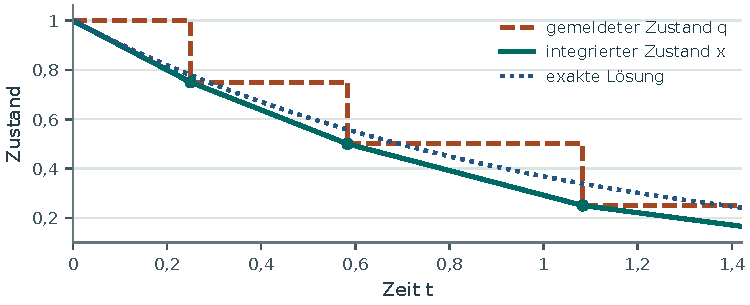
\includegraphics[width=.88\linewidth,height=49mm,keepaspectratio]{qss.pdf}\par}\capline{Die Meldung und der kontinuierliche Zustand haben verschiedene Aufgaben.}
\seite{}{QSS und DEVS}\anchorpage{2}{abs6-1}{6.1 · Quantisierung des Zustands}\ey{ABSCHNITT 6.1}\ptitle{Quantisierung des Zustands}
\hypertarget{punkt6-1-1}{}\subt{6.1.1\enspace Ein Zustand löst eine Meldung aus}
Zeitintegration plant einen Schritt und berechnet den neuen Zustand. QSS führt eine kontinuierliche Näherung \(x\) und ein an das Modell gemeldetes Signal \(q\). Es integriert \(x'=f(q)\) bis zur Grenze des Quantisierungsbandes. Komponenten mit nahezu konstanter Bewegung können lange dieselbe Meldung verwenden. Ob die Implementierung Zeit spart, hängt auch von den Abhängigkeiten und dem Aufwand pro Meldung ab.
\hypertarget{punkt6-1-2}{}\subt{6.1.2\enspace DEVS als Ereignisverwaltung}
Ein atomares DEVS-Modell besitzt Zustand, Ein- und Ausgabe, eine Zeitfortschrittsfunktion sowie interne und externe Übergänge. Der Koordinator wählt das kleinste Fälligkeitsdatum, erstellt die Ausgabe, verteilt Nachrichten und lässt die betroffenen Modelle ihre Termine aktualisieren. Gleichzeitige interne und externe Eingänge benötigen eine festgelegte Konfliktregel. Versionsmarken verhindern, dass ein überholter Eintrag aus der Warteschlange später ausgeführt wird.
\hypertarget{punkt6-1-3}{}\subt{6.1.3\enspace Absolute und relative Quanten}
Für den Speicher in Kelvin sei \(\Delta_i=\max(\Delta_{\min,i},r_i|q_i|)\). Das Band schrumpft beim Abkühlen, der absolute Boden verhindert unendlich kleine Zahlenabstände nahe null. Ein festes Quantum in Metern hat für eine Geschwindigkeit eine andere Bedeutung. Bei einem externen Impuls muss der nächste Termin aus dem neuen Zustand berechnet werden.
\lektion{Wie ein Zustand den nächsten Zeitpunkt bestimmt}{qss}{Kernweg}{Hybride Systeme}
Stellen Sie einer Uhr eine zweite Art von Melder gegenüber. Die Uhr meldet den nächsten vorgegebenen Zeitpunkt. Ein Quantisierer meldet, wann sich eine bestimmte Zustandskomponente um ihr vorgegebenes Quantum geändert hat. Hieraus bauen Quantized-State-System-Verfahren (QSS) eine Integration mit komponentenweise ausgelösten Aktualisierungen. Physikalische Schaltgrenzen kommen bei Bedarf zusätzlich hinzu.
\subt{QSS1 an einem Entladevorgang}
Ein normierter Speicher entlädt sich nach \(y'=-y,\ y(0)=1\). QSS1 integriert \(x'=-q\) und meldet einen konstanten Wert \(q\), bis \(|x-q|=\Delta\) erreicht ist. Beim eigenen Ereignis wird \(q\) auf \(x\) gesetzt. Für \(\Delta=1/4\) gilt zunächst \(x=1-t,\ q=1\). Bei \(t=1/4\) wird \(q=3/4\). Mit der neuen Steigung \(-3/4\) dauert das nächste Viertel im Zustand \(1/3\) Zeiteinheiten. Das zweite Ereignis liegt also bei \(t=7/12\). Die Zeitabstände folgen aus der lokalen Dynamik.
\fig{qss}{.9}{Die gemeldete Treppe bestimmt die Steigung der integrierten Kurve. Die gepunktete Referenz ist \(e^{-t}\). Auch wenn \(x\) und \(q\) nahe beieinanderliegen, ist die Abweichung von der exakten Lösung eine andere Größe.}
\subt{Woher der Ereignismechanismus kommt}
DEVS (\emph{Discrete Event System Specification}) beschreibt einen Baustein mit Zustand, Ein- und Ausgaben, interner und externer Übergangsfunktion, Ausgabefunktion und Zeit bis zum nächsten internen Ereignis. Ein Quantisierer kann so seine nächste Meldung ankündigen. Ändert ein anderer Baustein die Steigung, muss die Vorhersage neu berechnet werden. Für zeitgleiche Ereignisse benötigt das Modell eine eindeutige Regel.
\srcs{\refbk{devs}{Zeigler sowie Zeigler und Lee} · \refbk{qorig}{Kofman und Junco, Quantized-State Systems}.}

\seite{}{QSS und DEVS}\anchorpage{2}{abs6-2}{6.2 · QSS1 bis QSS4 und eine globale Fehlerschranke}\ey{ABSCHNITT 6.2}\ptitle{QSS1 bis QSS4 und eine globale Fehlerschranke}
\hypertarget{punkt6-2-1}{}\subt{6.2.1\enspace QSS1 hält die gemeldete Größe konstant}
Für \(x'=-q\) mit \(x(0)=q(0)=1\) und \(\Delta=0{,}2\) sinkt \(x\) zunächst linear mit Steigung \ensuremath{-}1. Die erste Meldung erfolgt nach 0,2 Zeiteinheiten bei \(x=0{,}8\). Die zweite Flugzeit beträgt \(0{,}2/0{,}8=0{,}25\). Der kontinuierliche Zustand bewegt sich auch zwischen den Meldungen.
\hypertarget{punkt6-2-2}{}\subt{6.2.2\enspace Polynome und die nächste positive Wurzel}
QSS2 meldet eine Gerade, QSS3 ein quadratisches und QSS4 ein kubisches Polynom. Der integrierte Zustand hat im idealen Taylor-Verfahren jeweils einen Grad mehr. Man bildet \(x_i(s)-q_i(s)\mp\Delta_i\), sucht die kleinste zulässige positive Wurzel und prüft die Richtung. Eine Wurzel nahe null unmittelbar nach einer Meldung braucht eine eigene Behandlung. Der konkrete QSS2-Termin steht auf S.\,\pagelink{qzahl}.
\hypertarget{punkt6-2-3}{}\subt{6.2.3\enspace Beweis am stabilen linearen Speicher}
Sei \(y'=-ay+u,\ x'=-aq+u,\ a>0\) und überall \(|q-x|\le\Delta\). Mit \(e=x-y\) folgt \(e'=-ae-a(q-x)\). Multiplikation mit \(e^{at}\) und Integration liefert
\[
 |e(t)|\le e^{-at}|e(0)|+a\Delta\int_0^te^{-a(t-s)}\,ds
 = e^{-at}|e(0)|+(1-e^{-at})\Delta .
\]
Die Schranke gilt für alle Zeiten des glatten Abschnitts. Sie beschreibt die gedämpfte Fehlerantwort. Zusätzliche numerische Ableitungs- und Resetfehler müssen separat eingehen.
\notebox{Merksatz}{Für einen stabilen linearen Vektorspeicher mit \(\|e^{At}\|\le M e^{-\gamma t}\), \(\gamma>0\), gilt bei \(\|q-x\|\le\Delta\) und \(e=x-y\) die Gleichung \(e'=Ae+A(q-x)\). Variation der Konstanten und Integration von \(e^{-\gamma(t-s)}\) ergeben \(\|e(t)\|\le M e^{-\gamma t}\|e(0)\|+M\|A\|\Delta(1-e^{-\gamma t})/\gamma\). Für gekoppelte Speicher kann der Verstärkungsfaktor größer als eins sein.}
\lektion{Wie der Quantisierungsfehler die Lösung stört}{qfehler}{Vertiefung}{Hybride Systeme}
Die diskrete Meldung \(q\) verändert die rechte Seite. Das Quantum hat die Einheit des zugehörigen Zustands. Ein Quantum von einem Millimeter bei der Position und eines von einem Ampere beim Strom sind ohne getrennte Skalierung unvergleichbar.
\subt{Satz · Fehlergrenze für einen stabilen skalaren Speicher}
Es gelte \(y'=-ay,\ x'=-aq,\ a>0,\ x(0)=y(0)\) und während des gesamten Versuchs \(|x-q|\le\Delta\). Dann gilt
\[
 |x(t)-y(t)|\le\Delta(1-e^{-at}).
\]
\proofpart{Mit \(e=x-y,\ \delta=x-q\) ergibt sich \(e'=-ae+a\delta\). Variation der Konstanten liefert \(e(t)=a\int_0^t e^{-a(t-s)}\delta(s)\dg s\). Der Betrag ist höchstens \(a\Delta\int_0^t e^{-a(t-s)}\dg s\). Auswerten des Integrals ergibt die Behauptung.}
Die Abschätzung nutzt die dämpfende skalare Gleichung. In gekoppelten Systemen wirkt ein Quantisierungsfehler über die Dynamik auf andere Komponenten. Ein kleines Quantum allein garantiert keine bestimmte Stoßzeit. Liegt ein Wächter fast tangential zur Bahn, kann schon eine kleine Zustandsabweichung die geschätzte Zeit stark verschieben.
\subt{Ein äußerer Eingang widerruft einen Termin}
Für \(x'=u\), \(x(0)=q(0)=0\), \(\Delta=1/4\), \(u=1\) ist die erste Meldung bei \(t=1/4\) vorgesehen. Bereits bei \(t=1/8\) springt der Eingang auf \(-1\). Dann steht \(x=1/8,\ q=0\). Die neue Grenze liegt bei \(-1/4\), also noch \(3/8\) Zeiteinheiten entfernt. Der nächste Meldetermin ist \(t=1/2\). Eine unverändert ausgelöste Meldung beim alten Termin wäre ein Fehler in der Ablaufsteuerung.
\notebox{Lokale Arbeit}{Ein Zustandsereignis verändert nur jene rechten Seiten, die den gemeldeten Zustand tatsächlich verwenden. Ein dünn besetzter Abhängigkeitsgraph spart Arbeit, wenn der Simulator lokale Aktualisierungen umsetzt und die Komponenten zu unterschiedlichen Zeiten aktiv sind. Der Python-Referenzcode im Projekt verwendet auch dichte Auswertungen.}
\srcs{\refbk{qorig}{QSS-Grundlage} · \refbk{qrev}{Übersicht zu QSS} · \repo{docs/SOLVER_SELECTION.md}{Implementierung und Kosten}.}

\lektion{Vom Quantum zur nächsten Meldung}{qzahl}{Rechenversuch}{Nachweise zum Modell}
\subt{QSS2 · Ein Fehlerpolynom von Hand auswerten}
Für \(x'=-q,\ x(0)=1\) meldet QSS2 anfangs Wert und Steigung, also \(q(t)=1-t\). Integration liefert \(x(t)=1-t+t^2/2\). Bei \(\Delta=0{,}02\) erreicht \(|x-q|=t^2/2\) erstmals im Zeitpunkt \(t=0{,}2\) das Quantum. Direkt davor gelten \(x=0{,}82\) und \(q=0{,}8\). QSS3 benutzt analog eine quadratische Meldung und eine kubische Bahn, bei der QSS4-Erweiterung steigen beide Grade um eins.
\subt{Drei Regeln am stabilen Speicher}
Für \(x'=-q\) und \(x(0)=100\) frieren wir die Meldung jeweils bis zum ersten Termin ein oder wählen vorab ihren Zielwert:
\begin{itemize}\zerolist
\item Relatives QSS1 meldet zunächst \(q=100\). Mit \(\max(0{,}01;0{,}1|x|)=10\) wird nach \(0{,}1\) bei \(x=90\) neu gemeldet. Dann beträgt das Quantum 9.
\item CQSS1 mit Zellbreite 10 meldet anfangs den Mittelpunkt 100. Die untere Fläche liegt bei 95. Sie wird nach \(0{,}05\) erreicht, dann meldet die folgende Zelle ihren Mittelpunkt 90.
\item BQSS1 prüft vor der Integration die Richtung und wählt für Quantum 10 das vorausliegende Ziel 90. Damit gilt \(x'=-90\), und das Ziel wird nach \(1/9\) erreicht. Zeigt die dort ausgewertete Steigung in einem gekoppelten Versuch weg vom Ziel, hält die Implementierung die Komponente bis zur nächsten möglichen Änderung an.
\end{itemize}
\srcs{\see{qkatalog}{Verfahrensübersicht} · \repocurrent{argesim_benchmarks/solvers/backward_qss.py}{Zielwahl und Halteregel}.}

\seite{}{QSS und DEVS}\anchorpage{2}{abs6-3}{6.3 · Steifigkeit und Chattering bei QSS}\ey{ABSCHNITT 6.3}\ptitle{Steifigkeit und Chattering bei QSS}
\hypertarget{punkt6-3-1}{}\subt{6.3.1\enspace Wenn ein schnelles Rückstellglied zu viele Meldungen erzeugt}
Liegt das Gleichgewicht einer stark gedämpften Komponente mitten im Band, kann die eingefrorene Steigung den Zustand darüber hinaustragen. Beim Melden wechselt das Vorzeichen. Der Speicher pendelt numerisch, obwohl das physikalische System rasch in Ruhe käme. Ein typischer Diagnoseversuch zeichnet \(x_i,q_i\) und die Meldedichte zusammen auf und verkleinert dann das Quantum. Numerische Meldungen und physikalische Schaltungen sind getrennte Zähler.

Rechnen Sie einen solchen Umlauf selbst. Für \(x'=-a q\), \(a>0\), verwendet QSS1 die Aktualisierung \(q\leftarrow x\), sobald \(|x-q|=\Delta\). Starten wir mit \(q=x=\Delta/2\). Die Steigung beträgt \(-a\Delta/2\). Um bis \(-\Delta/2\) zu reisen, muss \(x\) die Strecke \(\Delta\) zurücklegen. Das dauert \(\Delta/(a\Delta/2)=2/a\). Jetzt kehrt die Steigung ihr Vorzeichen um. Nach weiteren \(2/a\) ist der Ausgangswert wieder erreicht. Bei diesem gewählten Start halbiert ein halb so großes Band samt halbiertem Startwert die Schwingungsamplitude. Die Periodendauer \(4/a\) bleibt gleich. Die exakte Lösung \((\Delta/2)e^{-at}\) fällt dagegen fortlaufend.
\seite{}{QSS und DEVS}\anchorpage{2}{abs6-4}{6.4 · LIQSS und partitionierte Verfahren}\ey{ABSCHNITT 6.4}\ptitle{LIQSS und partitionierte Verfahren}
\hypertarget{punkt6-4-1}{}\subt{6.4.1\enspace Lokale implizite Rückkopplung}
LIQSS nähert die eigene Abhängigkeit als \(x_i'\simeq a_{ii}x_i+u_i\) an. Im Dämpfungsfall \(a_{ii}<0\) gibt \(-u_i/a_{ii}\) das lokale Gleichgewicht an. Die Quantisierungsentscheidung berücksichtigt es und kann die unphysikalische Banddurchquerung vermeiden. Bei zwei stark rückgekoppelten Zuständen enthält die Diagonale nur einen Teil der Dynamik. Eine Paarbehandlung oder ein Blocksolve kann angemessener sein.
\hypertarget{punkt6-4-2}{}\subt{6.4.2\enspace eLIQSS und die Bandbreite}
Erweiterte Quantisierer wählen das Startpolynom so, dass seine Differenz zum fortgeführten Zustand einen größeren zulässigen Teil des Bandes ausnutzt. Die erwartete Flugzeit wird unter den örtlichen Modellannahmen verlängert. Eine externe Nachricht kann jede Prognose vorzeitig beenden. Im Projekt ergeben eLIQSS1 und CheQSS1 dieselbe mathematische Aktualisierung.
\hypertarget{punkt6-4-3}{}\subt{6.4.3\enspace LIQSS–BDF über eine Blockgrenze}
In der Projektvariante übernimmt LIQSS2 die quantisierten Komponenten, BDF1/2 den angegebenen steifen Block. An der gemeinsamen Zeit müssen beide Blöcke mit verträglichen Kopplungswerten rechnen. Scheitert die Kopplungsiteration, darf kein Teilzustand vorzeitig festgeschrieben werden. Für den Vergleich zählen auch diese Iterationen, Neuplanungen und verworfenen Versuche.
\srcs{\repocurrent{docs/SOLVER_METHODS.md}{Quantisierer im Projekt} · \refbk{qorig}{Literatur zur Zustandsquantisierung}.}
\lektion{Die quantisierten Methoden im Vergleich}{qkatalog}{Vertiefung}{Hybride Systeme}
Die Ordnungszahl beschreibt die Konstruktion auf glatten Abschnitten. Bei explizitem QSS der Ordnung \(p\) hat der gemeldete Verlauf typischerweise Grad \(p-1\) und der integrierte Verlauf Grad \(p\). QSS2 kann damit eine freie Bewegung mit konstanter Geschwindigkeit auf dem jeweiligen Abschnitt darstellen. Ein physikalischer Kontakt muss weiterhin lokalisiert werden.
{\tblstart\begin{tabularx}{\linewidth}{@{}P{28mm}Y@{}}\toprule
\hd{Familie}&\hd{Rechenidee und geeigneter Versuch}\\\midrule
QSS1 bis QSS4&Konstante, lineare, quadratische oder kubische Meldung. Höhere Ordnung lohnt auf glatten Abschnitten, sofern zusätzliche Ableitungsarbeit und Nullstellensuche sich auszahlen.\\
CQSS1&Zentrierte Zelle ohne Hysterese. Für geeignete geometrische Systeme interessant. An Zellgrenzen können unmittelbare Rückwechsel den Zeitfortschritt verhindern.\\
LIQSS1 bis 3&Lokale lineare Selbstkopplung über den Diagonaleintrag der Jacobi-Matrix. Eine schnelle Komponente kann einem nahen Gleichgewicht folgen.\\
mLIQSS1 bis 3&Stark rückgekoppelte Paare werden gemeinsam behandelt. Das erhöht den Aufwand je Meldung. Die Variante dritter Ordnung ist eine experimentelle Projekterweiterung.\\
eLIQSS1 bis 3&Nutzt den vom Fehlerpolynom erlaubten Teil des Quantisierungsbands bis zum nächsten geplanten Ereignis.\\
CheQSS1 bis 3&Verteilt den Fehler mit verschobenen Tschebyscheff-Polynomen. In erster Ordnung ist die Aktualisierung dieselbe wie bei eLIQSS1.\\
LIQSS-BDF&Teilt Zustände in eine quantisierte und eine implizit zeitintegrierte Gruppe. Auf der BDF-Seite dienen rückwärts Euler und BDF2 als Schritte. Partition und Austausch müssen zur Kopplung passen.\\\bottomrule
\end{tabularx}\par}
Die Acht-Fälle-Matrix enthält damit 18 registrierte QSS-Namen. Die spätere Auswahlstudie ergänzt BQSS1, das vorwärts liegende Gitterwerte anhand der Bewegungsrichtung auswählt, sowie QSS1/2 mit logarithmischer Quantisierung. Dabei wird die Breite bei einem eigenen Update aus \(\max(\Delta_\mathrm{abs},\Delta_\mathrm{rel}|x_i|)\) bestimmt. Relative Quanten helfen bei großen Dynamikbereichen. Die absolute Untergrenze ist nahe null entscheidend.
\srcs{\repo{QSS_SOLVERS.md}{Methodenkatalog des Projekts} · \refbk{liq}{Migoni u.\,a., LIQSS} · \see{matrix}{alle 18 Namen und ihre Trefferzahlen} · \see{qzahl}{Drei Quantenregeln und der erste QSS2-Termin}.}
\lektion{Zwei Quantisierer melden gleichzeitig}{pruefung6}{Herleitung und Gegenprobe}{Kapitel 6}
Zwei Speicher werden mit der gleichen konstanten Rate geladen. Beide melden nach \(0{,}2\unitm s\) einen Banddurchgang. Ein dritter Baustein erhält die Differenz \(q_1-q_2\). In der richtigen Trajektorie ist diese Differenz null. Wenn das Programm die erste Meldung schon wirksam macht und erst später die zweite einsammelt, erzeugt es eine künstliche Zwischenstufe. Wie legt man fest, was „gleichzeitig“ im Rechner bedeutet?

Für diesen Lehrversuch sei \(x'_1=x'_2=1\), \(x'_3=q_1-q_2\) und \(x(0)=q(0)=0\) bei einheitlich skalierten Zuständen. QSS1 hält \(q_1,q_2\) zwischen ihren Meldungen konstant. Das Quantum sei jeweils \(0{,}2\). Bei \(t=0{,}2\) sind die kontinuierlichen Zustände \(x_1=x_2=0{,}2\). Beide quantisierten Ausgänge wechseln im gleichen Ereigniszeitpunkt auf \(0{,}2\). Für das anschließende offene Zeitintervall ist also \(x'_3=0\). Bei \(t=0{,}4\) wiederholt sich die Rechnung. Wer nach der ersten Meldung \(x'_3=0{,}2\) findet, muss beim zweiten Eingang am gleichen Zeitpunkt die Prognose erneut bilden. Für das Fortschreiben von \(x_3\) ist dabei null physikalische Zeit vergangen.

Der Koordinator sammelt alle für denselben Termin gültigen internen Ausgaben aus dem alten Zustand, verteilt sie als Eingabemenge und führt erst dann die Zustandsübergänge aus. Treffen interne und externe Termine eines Bausteins zusammen, legt seine konfluente Übergangsfunktion die gemeinsame Verarbeitung fest. Zeitstempel mit einem zusätzlichen Mikroindex ordnen Folgereaktionen bei derselben physikalischen Zeit.
\notebox{Achtung, Falle}{Das willkürliche Zusammenziehen numerisch naher, tatsächlich verschiedener Zeiten kann die Ereignisfolge ändern. Im Versuch lassen sich die gemeinsamen Termine über denselben ganzzahligen Taktindex erzeugen. Prüfen Sie die dritte Trajektorie noch einmal bei umgekehrter Einfügereihenfolge der Meldungen.}
\srcs{\see{alg6}{Veraltete Termine im Kalender} · \see{qfehler}{Vom Quantenband zur globalen Fehlerschranke}.}

\lektion{Eine überholte QSS-Meldung erkennen}{alg6}{Werkstatt}{Kapitel 6}
Eine alte Prognose kann beim Eintreffen einer Nachricht noch in der Prioritätswarteschlange liegen. Verwaltet jeder Speicher eine fortlaufende Versionsnummer, erkennt der Koordinator veraltete Einträge, bevor sie den Zustand verändern.
{\small\begin{verbatim}
(t, i, version) = fruehester_Eintrag()
wenn version != aktuell[i]: ueberspringe_Eintrag
sammle_alle_gueltigen_Meldungen_zur_selben_Zeit(t)
fuehre_Polynome_bis(t)
sende interne Ausgaben aus den Zustaenden vor dem Wechsel
sammle fuer jedes Modell alle eintreffenden Eingaben
intern und extern: verwende die konfluente Modellregel
sonst: verwende den internen oder externen Uebergang
fuer jede betroffene Komponente j:
    aktuell[j] += 1
    plane(neuen_Banddurchgang(j), j, aktuell[j])
\end{verbatim}}
\subt{Selbst rechnen}
Ein Speicher erwartet den nächsten Durchgang bei 0,45 s. Um 0,3 s setzt eine externe Nachricht seine Steigung auf null. Wann darf der alte Durchgang den Zustand verändern?
\notebox{Lösung}{Mit der neuen Version ist der Termin bei 0,45 s ungültig. Bleibt der Zustand strikt im Band und die Steigung null, ist die nächste interne Zeit unendlich. Erst eine weitere Eingabe kann einen neuen endlichen Termin erzeugen.}

\seite{}{Räumliche Diskretisierung}\anchorpage{1}{neu7}{7 · Räumliche Diskretisierung partieller Differentialgleichungen}\ey{KAPITEL 7}\ptitle{Räumliche Diskretisierung partieller Differentialgleichungen}
Ein Ende eines Stabes wird heiß, das andere bleibt kühl. Ein einziges Thermometer kann den Wärmestrom zwischen beiden nicht bestimmen. Was ändert sich, wenn wir immer mehr Thermometer im Stab verteilen, und an welcher Stelle im Rechenweg erfordert die feinere Ortsauflösung plötzlich kürzere Zeitschritte?
\subt{Der Weg durch das Kapitel}
{\tblstart\begin{tabularx}{\linewidth}{@{}Yr@{}}\toprule
\hyperlink{abs7-1}{7.1 · Linienmethode und Randbedingungen} & \pagelink{abs7-1}\\[2pt]
\hyperlink{abs7-2}{7.2 · Finite Differenzen und diffusive Zeitskalen} & \pagelink{abs7-2}\\[2pt]
\hyperlink{abs7-3}{7.3 · Finite Volumen und hyperbolischer Transport} & \pagelink{abs7-3}\\[2pt]
\hyperlink{abs7-4}{7.4 · Finite Elemente und schwache Form} & \pagelink{abs7-4}\\[2pt]
\bottomrule\end{tabularx}\par}
\par\vfill{\centering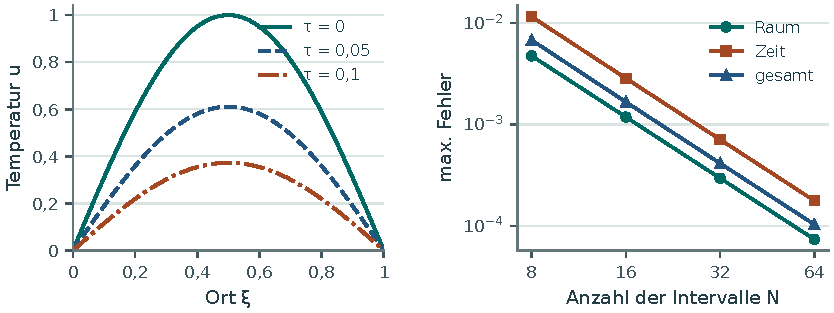
\includegraphics[width=.88\linewidth,height=49mm,keepaspectratio]{mol.pdf}\par}\capline{Nach der Ortsdiskretisierung wird jeder innere Knoten zu einer Zustandskomponente.}
\seite{}{Räumliche Diskretisierung}\anchorpage{2}{abs7-1}{7.1 · Linienmethode und Randbedingungen}\ey{ABSCHNITT 7.1}\ptitle{Linienmethode und Randbedingungen}
\hypertarget{punkt7-1-1}{}\subt{7.1.1\enspace Orts- und Zeitdiskretisierung trennen}
Schneiden wir den Stab in kleine Abschnitte. Jede Temperatur erhält eine Speicherbilanz, jeder Kontakt eine Austauschregel. So entsteht aus \(u_t=\kappa u_{xx}\) nach Wahl der Ortsdiskretisierung das System \(U'=A_hU+b(t)\). Erst jetzt fällt die Wahl des Zeitintegrators. Ein zweiter Versuch mit gleichem Ortsgitter und engeren Zeittoleranzen untersucht gezielt den Zeitfehler.
\hypertarget{punkt7-1-2}{}\subt{7.1.2\enspace Dirichlet, Neumann, Robin und Geisterpunkte}
Ein Bad hält die Randtemperatur fest (Dirichlet), eine Isolierung setzt den Wärmestrom auf null (Neumann), die Kühlung an Luft verknüpft Temperatur und Strom (Robin). Für zentrierte Differenzen an einem Randknoten und \(u_x(0)=0\) folgt aus \((U_1-U_{-1})/(2h)=0\) der Geisterwert \(U_{-1}=U_1\). Am zellzentrierten Rand liegt die Wand eine halbe Zelle entfernt. Dieselbe Indexformel hätte dort eine andere Geometrie.
\seite{Rechenbeispiel}{Räumliche Diskretisierung}\anchorpage{2}{kap6}{Was verraten drei Temperatursensoren?}\ptitle{Was verraten drei Temperatursensoren?}


\lernziel{Sie können eine Temperatur an einem Gitterpunkt fortschreiben, die Einheiten kontrollieren und begründen, warum die räumliche Auflösung den Zeitintegrator beeinflusst.}
Ein Sensor im Innern eines Stabes zeigt \(30\,^\circ\mathrm C\). Ein Zentimeter links davon messen wir \(20\,^\circ\mathrm C\), ein Zentimeter rechts \(24\,^\circ\mathrm C\). Der Heizer ist aus. Wird der mittlere Sensor als Nächstes wärmer oder kälter?
\minifig{dreipunkte}{29mm}{Die Nachbarn sind kälter als die Mitte. Der linke Temperaturunterschied ist größer. Beide Seiten tragen zum Abkühlen der Mitte bei.}
\subt{Was die Nachbarn zur nächsten Steigung beitragen}
Bei konstanter Temperaturleitfähigkeit \(\alpha=0{,}10\unitm{cm^2/s}\) schätzen wir die zweite Ortsableitung durch die Differenz der benachbarten Steigungen. Für die Mitte liefert das
\[
 \dot T_0\approx\alpha\frac{[(24-30)-(30-20)]\unitm K}{(1\unitm{cm})^2}
                 =-1{,}6\unitm{K/s}.
\]
Ein expliziter Euler-Schritt von einer Sekunde ergibt \(28{,}4\,^\circ\mathrm C\). Für alle inneren Punkte gleichzeitig entstehen solche Zeitgleichungen. Genau dieser Übergang von einem räumlichen Feld zu einem System von Zeitgleichungen heißt \emph{Linienmethode}.
\notebox{Vor dem Weiterblättern}{Erhöhen wir alle drei Messwerte um \(5\unitm K\), welche Zahl ändert sich? Die Differenzen und die Steigung bleiben gleich. Nur die neue Temperatur steigt ebenfalls um fünf Kelvin. Eine Rechnung, die jetzt schneller abkühlt, verletzt die angenommene Wärmeleitung.}

\srcs{\textbf{Kernweg}\enspace\see{mol}{Ortsgitter von Hand}\quad\see{molweg}{MOL und Methodenwahl}\quad\see{schwach}{Schwache Form}\quad\see{ueb6}{Selbst prüfen}.}

\lektion{Feld, Randwert und räumliche Ableitung lesen}{feldsprache}{Kernweg}{Felder und Linienmethode}
Eine Messsonde fährt nicht durch den Stab, sie bleibt an ihrem Ort \(x\). Ihre Anzeige im Lauf der Zeit ist \(T(x,t)\) bei festem \(x\). Die Änderung pro Sekunde heißt \(T_t\). Eine Reihe von Sensoren zur gleichen Zeit misst dagegen eine räumliche Steigung \(T_x\) in \(\mathrm{K/m}\). Die Änderung dieser Steigung pro Ortslänge heißt \(T_{xx}\) in \(\mathrm{K/m^2}\). Beim Profil \(T=20+ax^2e^{-bt}\) ergeben sich \(T_x=2ax e^{-bt}\) und \(T_{xx}=2ae^{-bt}\).
\subt{Was wird am Rand vorgegeben?}
Ein \emph{Dirichlet-Rand} schreibt einen Feldwert vor, etwa \(T(0,t)=20\,^\circ\mathrm C\). Ein \emph{Neumann-Rand} schreibt den Normalgradienten bzw. bei bekannter Leitfähigkeit den Fluss vor. Eine isolierte Stirnfläche hat verschwindenden Wärmefluss. Ein \emph{Robin-Rand} verbindet Wert und Fluss, beispielsweise \(-kA T_x(L,t)=G(T(L,t)-T_a)\). Diese Gleichungen beschreiben verschiedene Befestigungen des gleichen Körpers.
\subt{Vom Punkt zum kleinen Volumen}
In mehreren Dimensionen sammelt der \emph{Gradient} \(\nabla T\) alle räumlichen ersten Ableitungen. Die \emph{Divergenz} eines Flusses \(\mathbf j\) ist \(\nabla\cdot\mathbf j=\sum_i\partial j_i/\partial x_i\). Sie misst den lokalen Nettoausfluss pro Volumen. Bei konstanter Leitfähigkeit beschreibt \(\Delta T=\nabla\cdot\nabla T\) die Summe der zweiten Ableitungen. In einer Raumdimension ist das einfach \(T_{xx}\).

Bei Integration über eine Zelle werden die räumlichen Ableitungen zu Randflüssen. In einer Dimension ist das der Hauptsatz \(\int_a^b j_x\dg x=j(b)-j(a)\). In mehreren Dimensionen verknüpft der Gaußsche Integralsatz das Volumenintegral der Divergenz mit dem nach außen gerichteten Fluss durch die Oberfläche. Deshalb kann man im Finite-Volumen-Verfahren jede Zellgrenze genau einmal berechnen und mit entgegengesetzten Vorzeichen verbuchen.
\notebox{Ein Modell ist erst mit seinen Daten bestimmt}{Für die Wärmeleitung im Stab gehören das ganze anfängliche Temperaturprofil und die beiden Randbedingungen zum Problem. Zwei Anfangstemperaturen an den Enden legen die anfängliche Temperatur in der Mitte noch nicht fest.}

\lektion{Aus einer lokalen Bilanz wird ein Feldmodell}{pde}{Kernweg}{Felder und Linienmethode}
\vorhersage{6}{Wir halbieren die Zellbreite bei eindimensionaler Wärmeleitung. Wie ändert sich die Schrittgrenze für nichtnegative Euler-Gewichte?}{kontrolleA}
Schneiden Sie gedanklich ein kurzes Stück \([x,x+\Delta x]\) aus dem Stab. Im Innern speichern Masse und Wärmekapazität ungefähr \(\rho c A\Delta x\,T\) an Energie relativ zu einem festen Bezug. Von links kommt \(q(x)=-kA T_x(x)\), rechts geht \(q(x+\Delta x)\) ab. Hinzu kommt \(P\Delta x/L\) vom Heizer. Teilen durch die Stücklänge und der Grenzübergang liefern die lokale Bilanz
\[
 \rho cA\,T_t=-q_x+P/L=kA\,T_{xx}+P/L .
\]
Jeder Term hat die Einheit Watt pro Meter. Anfangs gilt \(T(x,0)=T_a\). Der isolierte linke Rand liefert \(T_x(0,t)=0\) (Neumann). Rechts liefert die Kontaktkette \(-kA T_x(L,t)=(T(L,t)-T_a)/R\) (Robin). Eine fest vorgegebene Endtemperatur wäre eine Dirichlet-Bedingung.
\subt{Die stationäre Lösung liefert einen unabhängigen Prüfwert}
Im Gleichgewicht gilt \(kA T''=-P/L\). Die linke Randbedingung ergibt \(T'(x)=-Px/(kAL)\). Rechts tritt deshalb genau \(P\) aus. Die Robin-Bedingung liefert \(T(L)=T_a+PR\). Nochmalige Integration ergibt
\[
 T(x)=T_a+PR+\frac{P}{2kAL}(L^2-x^2).
\]
Mit den Daten aus Kapitel 1 sind das \(60{,}00\,^\circ\mathrm C\) am Kontakt zum Stab und \(61{,}25\,^\circ\mathrm C\) an der isolierten Stirnseite. Räumliches Mitteln liefert \(60{,}8333\,^\circ\mathrm C\). Der masselose Zwischenkontakt hat weiterhin \(50\,^\circ\mathrm C\). Alle vier Werte beschreiben verschiedene Messorte oder Mittelungen.
\notebox{Entscheidung}{Gilt am heißen Ende eine zulässige Modellabweichung von \(0{,}5\unitm K\), genügt die Ein-Speicher-Näherung im Dauerbetrieb nicht. Ein beliebig genauer Zeitintegrator für dieses eine Temperaturmodell würde weiterhin \(60\,^\circ\mathrm C\) liefern.}
\srcs{\see{speicher}{Aufwärmkurve des konzentrierten Modells} · \refbk{fnc}{Driscoll und Braun, Linienmethode}.}

\lektion{Die Linienmethode von Hand}{mol}{Kernweg}{Felder und Linienmethode}
Wir richten einen gesonderten Prüfstand für das Ortsgitter ein. Der Heizer wird ausgeschaltet und \emph{beide} Enden werden jetzt auf Umgebungstemperatur gehalten. Mit \(\xi=x/L,\ \tau=\alpha t/L^2,\ \alpha=k/(\rho c)\) und \(u=(T-T_a)/\Delta T\) mit positivem Bezugshub \(\Delta T\) lautet die dimensionslose Wärmegleichung
\[
 u_\tau=u_{\xi\xi},\quad u(0,\tau)=u(1,\tau)=0,\quad
 u(\xi,0)=\sin(\pi\xi).
\]
Einsetzen bestätigt \(u(\xi,\tau)=e^{-\pi^2\tau}\sin(\pi\xi)\). Mit diesen geänderten Randdaten besitzt auch die zeitabhängige Rechnung eine exakte Referenz.
\subt{Erst den Ort diskretisieren}
Auf \(N\) gleich langen Intervallen sei \(\Delta\xi=1/N,\ U_j(\tau)\approx u(j\Delta\xi,\tau)\). Addieren der Taylorreihen um \(\xi_j\) hebt die ungeraden Potenzen auf. Damit ist
\[
 \frac{u(\xi_j-\Delta\xi)-2u(\xi_j)+u(\xi_j+\Delta\xi)}{\Delta\xi^2}
 =u''(\xi_j)+\frac{\Delta\xi^2}{12}u^{(4)}(\xi_j)+O(\Delta\xi^4)
\]
für hinreichend glatte Profile. Die inneren \(N-1\) Werte erfüllen jetzt \(\dot U_j=(U_{j-1}-2U_j+U_{j+1})/\Delta\xi^2\) bei \(U_0=U_N=0\). Die Zeit ist weiterhin kontinuierlich. Diese Trennung heißt Linienmethode (\emph{method of lines}, MOL).
\subt{Dann einen Zeitschritt ausrechnen}
Für vier Intervalle ist \(U(0)=(\sqrt2/2,1,\sqrt2/2)^\mathsf T\). Wir wählen vorwärts Euler mit \(\Delta\tau=0{,}025\), also \(r=\Delta\tau/\Delta\xi^2=0{,}4\). Der mittlere Wert wird zu \(1+0{,}4(\sqrt2-2)=0{,}765685\). Der linke und der rechte Innenwert werden jeweils \(0{,}541421\). Alle liegen zwischen null und eins.
\minifig{gitter4}{25mm}{Vier Intervalle ergeben drei dynamische Innenwerte. Die offene Punktreihe zeigt die Anfangswerte, die Quadrate die drei neuen Werte und die beiden festen Randwerte.}
\notebox{Wo entsteht eine DAE?}{Für den ursprünglichen Stab kann man Flüsse und die unbekannte Kontakttemperatur auf dem Gitter mitführen. Ihre algebraischen Kontaktgleichungen erzeugen Nullzeilen im zeitlichen Massenoperator. Werden sie vorab eliminiert, entsteht hier ein reines ODE-System.}
\srcs{\refbk{fnc}{FNC, The method of lines} · \see{fem}{Massenmatrix bei finiten Elementen}.}

\lektion{Zwei Zellen und ein masseloser Rand}{molrand}{Vertiefung}{Felder und Linienmethode}
Nun kombinieren wir am beheizten Originalstab die Linienmethode mit der algebraischen Kontaktbedingung. Zwei gleich große Kontrollvolumen haben je \(C/2=60\unitm{J/K}\) und erhalten je \(P/2=5\unitm W\). Ihre Temperaturüberschüsse \(U_1,U_2\) sitzen in den Zellzentren. Zwischen den Zentren ergibt Fourier \(q_{12}=(U_1-U_2)/R_{12}\) mit \(R_{12}=\Delta x/(kA)=0{,}125\unitm{K/W}\).

Rechts liegt vom zweiten Zentrum bis zur Stirnfläche noch eine halbe Zelle. Ihr Wärmewiderstand ist \(R_h=\Delta x/(2kA)=0{,}0625\unitm{K/W}\). Damit entsteht die semidiskrete DAE
\[
 \begin{aligned}
 60\dot U_1&=5-q_{12},& 60\dot U_2&=5+q_{12}-q_R,\\
 U_2-\theta_s&=(R_h+R_1)q_R,& \theta_s&=R_2q_R .
 \end{aligned}
\]
Der Zwischenstrom hebt sich beim Addieren beider Speicherbilanzen auf. Startwerte sind \(U_1=U_2=\theta_s=q_R=0\). Eliminiert man die masselosen Kontaktgrößen, folgt \(q_R=U_2/(R_h+R_1+R_2)=U_2/4{,}0625\). Die verbleibenden zwei Gleichungen sind eine ODE.
\subt{Ein Schritt mit Zahlen}
Nach einem Rückwärts-Euler-Schritt von \(60\unitm s\) folgt
\[
 \begin{bmatrix}9&-8\\-8&9+1/4{,}0625\end{bmatrix}
 \begin{bmatrix}U_1\\U_2\end{bmatrix}=\begin{bmatrix}5\\5\end{bmatrix}.
\]
Einsetzen liefert \(U_1=4{,}48759\unitm K,\ U_2=4{,}42354\unitm K\) und \(q_R=1{,}08887\unitm W\). Der rechte Zellmittelpunkt ist kälter, wie die einseitige Kühlung erwarten lässt. Die Speicher nehmen zusammen \(8{,}91113\unitm W\) auf. Mit dem Randstrom sind dies die zugeführten \(10\unitm W\), bis auf Rundung.
\notebox{Modellentscheidung im Detail}{MOL legt hier die räumliche Darstellung fest, die Zeitschrittformel setzt den Zeitfehler. Die Entscheidung, am Rand \(q_R,\theta_s\) gemeinsam zu lösen oder explizit einzusetzen, verändert die Solver-Schnittstelle. Die eliminierte und die simultan gelöste diskrete Form liefern bei exakter linearer Lösung dieselben Temperaturen.}

\lektion{Welche Entscheidung trifft die Linienmethode?}{molweg}{Methodenwahl}{Vom Feld zum Solver}
\textbf{Auftrag.} Für einen dünnen Stab sollen die Temperaturen in der Mitte und nahe dem rechten Ende als Funktion der Zeit berechnet werden. In der Feldgleichung \(T_t=\alpha T_{xx}\) bezeichnet \(T(x,t)\) noch eine Temperatur an jedem Ort und zu jeder Zeit.
\subt{Was übergeben wir an den Zeitintegrator?}
Wählen wir drei gleich weit entfernte innere Messorte und halten beide Enden bei \(0\,^{\circ}\mathrm C\), so wird aus dem Feld ein Vektor \(U=(T_1,T_2,T_3)^\top\). Die \emph{method of lines} (MOL, Linienmethode) ersetzt die räumlichen Ableitungen. An jedem festen Ort bleibt eine stetige Zeitvariable. Für zentrale Differenzen ergibt sich
\[
 \dot U=\frac{\alpha}{\Delta x^2}
 \begin{pmatrix}-2&1&0\\1&-2&1\\0&1&-2\end{pmatrix}U.
\]
Bei \(U=(0,10,0)^\top\,\mathrm K\) als Überschuss und \(\alpha/\Delta x^2=0{,}1\,\mathrm{s}^{-1}\) liefert die Modellfunktion \((1,-2,1)^\top\,\mathrm{K/s}\). Erst Euler etwa mit \(h=1\,\mathrm s\) erzeugt den nächsten Zustand \((1,8,1)^\top\,\mathrm K\).
\subt{Andere Raumdarstellungen führen zur selben Zeitfrage}
{\tblstart\begin{tabularx}{\linewidth}{@{}P{27mm}YY@{}}\toprule
\hd{Raumverfahren}&\hd{Was wird gespeichert?}&\hd{Woran prüfe ich das Ergebnis?}\\\midrule
Differenzen&Knotenwerte. Steigungen aus Nachbarn.&Fehlerabnahme bei Gitterverfeinerung.\\
Finite Volumen&Zellmittelwerte. Flüsse über gemeinsame Flächen.&Zu- und Abfluss jeder Zelle.\\
Finite Elemente&Koeffizienten lokaler Basisfunktionen in der schwachen Form.&Randbedingungen, Energie und Gitterfehler.\\
Spektralverfahren&Koeffizienten globaler Moden.&Abklingen hoher Moden bei glatten Daten.\\\bottomrule
\end{tabularx}\par}
Mit finiten Elementen entsteht oft \(M\dot U=r(t,U)\). Ist die Massenmatrix \(M\) invertierbar, ergibt das Lösen eines linearen Systems die Rate. Bleibt ein masseloser Rand als algebraische Unbekannte erhalten, gehören eine Nebenbedingung und passende Anfangswerte zum DAE-Problem.
\srcs{\href{https://fncbook.com/methodlines/}{Driscoll und Braun, Method of Lines} · \see{molrand}{Ein Rand mit algebraischer Bindung} · \see{schwach}{Schwache Form}.}

\lektion{Parabolisch, hyperbolisch oder elliptisch?}{pdearten}{Kernweg}{Felder und Linienmethode}
Der stationäre Temperaturverlauf des Stabs und seine Aufheizkurve haben verschiedene mathematische Strukturen. Auch die Ausbreitung eines Signals kann ein Feldmodell verlangen. Für die folgenden klassischen Prototypen gibt die Physik den ersten Hinweis.
{\tblstart\begin{tabularx}{\linewidth}{@{}P{27mm}Y@{}}\toprule
\hd{Prototyp}&\hd{Daten, Verhalten und numerische Folge}\\\midrule
Diffusion, parabolisch \(u_t=\alpha u_{xx}\)&Anfangsprofil und passende Randdaten. Kurze Wellen klingen besonders schnell ab. Nach MOL wächst der Betrag des schnellsten Eigenwerts wie \(\Delta x^{-2}\).\\
Welle, hyperbolisch \(u_{tt}=a^2u_{xx}\)&Auslenkung und Geschwindigkeit zu Beginn, dazu passende Randbedingungen. Signale laufen mit endlicher Geschwindigkeit. Phasengang und Energie sind Prüfgrößen.\\
Poisson, elliptisch \(-\nabla\cdot(k\nabla u)=f\)&Randwertproblem im Raum. Eine stationäre Temperatur braucht keine physikalische Anfangszeit. Nach der Diskretisierung wird ein algebraisches Gleichungssystem gelöst.\\\bottomrule
\end{tabularx}\par}
\subt{Ein Netzgleichgewicht konkret lösen}
Beim Stab im Dauerbetrieb verschwindet die Speicherrate. In der FEM-Darstellung bleibt \(KU=b\). Als Beispiel genüge ein lineares Element über die gesamte Länge. Sein Wärmeleitwert beträgt \(kA/L=4\unitm{W/K}\), bei \(k=200\unitm{W/(m\,K)}\) als Wärmeleitfähigkeit des Materials. Bei doppelter Länge und unverändertem Querschnitt beträgt der Leitwert \(2\unitm{W/K}\). Mit \(G=0{,}25\unitm{W/K}\) und gleich verteilter Leistung \(P=10\unitm W\) entsteht
\[
 \begin{bmatrix}4&-4\\-4&4{,}25\end{bmatrix}
 \begin{bmatrix}\theta_0\\ \theta_L\end{bmatrix}
 =\begin{bmatrix}5\\5\end{bmatrix}.
\]
Addition der Zeilen liefert \(0{,}25\theta_L=10\). Rückeinsetzen gibt \(\theta_0=41{,}25\unitm K,\ \theta_L=40\unitm K\). Beide Knotenwerte treffen hier die exakte Lösung. Dazwischen verbindet das Element sie linear, während das exakte Profil quadratisch ist. Ein Vergleich allein an den Randknoten übersieht den Fehler im Inneren.
\notebox{Alternative zum Zeitmarsch}{Bei einer positiv definiten stationären Matrix passen Cholesky oder vorkonditionierte konjugierte Gradienten. Ein rein isolierter Stab mit positiver dauernder Heizleistung besitzt kein stationäres Gleichgewicht. Eine Verträglichkeitsprüfung gehört vor die Wahl des Lösers.}

\seite{}{Räumliche Diskretisierung}\anchorpage{2}{abs7-2}{7.2 · Finite Differenzen und diffusive Zeitskalen}\ey{ABSCHNITT 7.2}\ptitle{Finite Differenzen und diffusive Zeitskalen}
\hypertarget{punkt7-2-1}{}\subt{7.2.1\enspace Der zentrale Diffusionsoperator}
Die Flüsse von links und rechts unterscheiden sich um eine weitere Differenz. Für den inneren Punkt gilt \(U'_j=\kappa(U_{j-1}-2U_j+U_{j+1})/h_x^2\). Einsetzen eines konstanten Profils ergibt null. Einsetzen von \(x^2\) ergibt exakt \(2\kappa\). Die Taylor-Reste der Nachbarn zeigen für glatte Profile einen Ortsfehler zweiter Ordnung.
\hypertarget{punkt7-2-2}{}\subt{7.2.2\enspace Warum Halbieren des Gitters vier Schritte kostet}
Der alternierende Gittermodus \((1,-1,1,-1,\ldots)\) trägt auf dem periodischen geraden Gitter den Eigenwert \(-4\kappa/h_x^2\). Damit fordert Vorwärts-Euler \(h_t\le h_x^2/(2\kappa)\). Halbiert man \(h_x\), vervierfacht sich die Zahl der Zeitschritte auf demselben Intervall. Ein impliziter Integrator kann diese Stabilitätsgrenze überwinden. Die räumliche Genauigkeit und das Budget für die linearen Lösungen bleiben zu prüfen.
\lektion{Warum ein feineres Gitter steifer wird}{gitterstabil}{Kernweg}{Felder und Linienmethode}
Wie groß darf ein Zeitschritt sein, wenn keine neue heißeste oder kälteste Stelle entstehen soll? Sammeln wir am Innenknoten alle Koeffizienten der alten Temperaturen. Der explizite Diffusionsschritt lautet
\[
 U_j^{n+1}=rU_{j-1}^n+(1-2r)U_j^n+rU_{j+1}^n .
\]
Für \(0\le r\le1/2\) sind alle Gewichte nichtnegativ und addieren sich zu eins. Jeder neue Wert liegt damit im Bereich seiner Nachbarn einschließlich des eigenen alten Werts. Per Induktion bleiben die globalen Extremwerte bei homogenen Dirichlet-Rändern durch die Extremwerte aus Start und Rand beschränkt. Das ist das diskrete Maximumprinzip.
\subt{Beweis der spektralen Schranke}
Die Gitterfunktion \(v_j=\sin(k\pi j/N)\) verschwindet an beiden Enden. Aus \(\sin(a-b)+\sin(a+b)=2\sin(a)\cos(b)\) folgt
\[
 (D_{xx}v)_j=\lambda_k v_j,\qquad
 \lambda_k=-4N^2\sin^2\!\left(\frac{k\pi}{2N}\right),\quad 1\le k<N.
\]
Die Sinusmoden bilden eine orthogonale Basis. Jede Amplitude wird durch Euler mit \(1+\Delta\tau\lambda_k\) multipliziert. Die größtmögliche Frequenz \(k=N-1\) bestimmt deshalb die exakte Stabilitätsgrenze in der euklidischen Norm:
\[
 r\le\frac{1}{2\cos^2(\pi/(2N))}.
\]
Für ein endliches Gitter liegt sie geringfügig über \(1/2\). Die einfachere Schranke \(r\le1/2\) sichert zusätzlich das Maximumprinzip. Wenn \(\Delta\xi\) halbiert wird, muss für diese explizite Bedingung \(\Delta\tau\) geviertelt werden.
\subt{Was ein impliziter Schritt ändert}
Bei rückwärts Euler wird \((I-\Delta\tau D_{xx})U^{n+1}=U^n\) gelöst. Die Matrix ist tridiagonal. Radau und BDF können dieselbe lokale Kopplungsstruktur nutzen. Die implizite Dämpfung befreit von der obigen linearen Euler-Schranke. Soll gerade der Abbau einer schnellen Mode genau aufgelöst werden, bleibt ihre Zeitskala wichtig.
\task{4}{Für \(\alpha=10^{-4}\,\mathrm{m^2/s}\) und \(\Delta x=2\unitm{cm}\) bestimmen Sie einen maximalen Euler-Schritt nach dem Maximumprinzip. Was gilt bei halbem Gitterabstand?}

\lektion{Raum- und Zeitfehler einzeln messen}{raumfehler}{Kernweg}{Felder und Linienmethode}
Wir beobachten den sinusförmigen Prüfstand bei \(\tau_f=0{,}1\). Die PDE liefert \(u^*(\xi)=e^{-\pi^2\tau_f}\sin(\pi\xi)\). Für jedes Gitter kennen wir außerdem die \emph{exakte Lösung des räumlich diskreten Systems}, \(U_j^h=e^{\lambda_1\tau_f}\sin(\pi j/N)\). Schließlich berechnet vorwärts Euler \(U_j^{h,k}\) bei \(r=0{,}4\). Damit stehen zwei unabhängige Vergleiche zur Verfügung.
{\tblstart\begin{tabularx}{\linewidth}{@{}rrYYY@{}}\toprule
\hd{\(N\)}&\hd{Schritte}&\hd{Raumfehler}&\hd{Zeitfehler}&\hd{Gesamtfehler}\\\midrule
8&16&\(4{,}733\cdot10^{-3}\)&\(1{,}150\cdot10^{-2}\)&\(6{,}762\cdot10^{-3}\)\\
16&64&\(1{,}182\cdot10^{-3}\)&\(2{,}846\cdot10^{-3}\)&\(1{,}663\cdot10^{-3}\)\\
32&256&\(2{,}955\cdot10^{-4}\)&\(7{,}097\cdot10^{-4}\)&\(4{,}142\cdot10^{-4}\)\\
64&1024&\(7{,}386\cdot10^{-5}\)&\(1{,}773\cdot10^{-4}\)&\(1{,}034\cdot10^{-4}\)\\\bottomrule
\end{tabularx}\par}
\capline{Maximumnorm über alle inneren Knoten. Raumfehler \(\|U^h-u^*\|_\infty\), Zeitfehler \(\|U^{h,k}-U^h\|_\infty\), Gesamtfehler \(\|U^{h,k}-u^*\|_\infty\).}
\fig{mol}{.95}{Links bleibt die Form der Grundmode erhalten. Rechts sinken die Fehler bei Gitterverdopplung etwa auf ein Viertel. Hier wird gleichzeitig der Zeitschritt geviertelt.}
\subt{Weshalb der Gesamtfehler kleiner als der Zeitfehler ist}
Für die Grundmode ist \(|\lambda_1|<\pi^2\), das Ortsgitter dämpft also zu schwach. Euler dämpft diese Mode im gewählten Bereich zu stark, denn \(0<1+z<e^z\) bei \(-1<z<0\). Die Fehler wirken gegeneinander. Aus dem Gesamtfehler allein ließe sich diese Kompensation nicht erkennen. Die beobachtete Ordnung nahe zwei gegenüber \(\Delta\xi\) ist mit dem Zeitfehler erster Ordnung bei \(\Delta\tau=0{,}4\Delta\xi^2\) vereinbar.
\srcs{Eigener Rechenversuch · expliziter Dreipunktoperator in \texttt{molexperiment}, gegengeprüft mit der analytischen Verstärkung jeder Rechnung.}

\lektion{Ein Energiebeweis für die Wärmegleichung}{waermebeweis}{Vertiefung}{Felder und Linienmethode}
Könnten zwei verschiedene Temperaturfelder dieselbe Geometrie, Heizleistung, Anfangstemperatur und Randbedingung erfüllen? Für hinreichend glatte Lösungen \(T_1,T_2\) betrachten wir ihre Differenz \(w=T_1-T_2\). Die Quelle fällt heraus. Links bleibt \(w_x(0,t)=0\), rechts \(-kAw_x(L,t)=G w(L,t)\) mit \(G=1/R>0\).
\subt{Satz · Eindeutigkeit bei gekühltem Rand}
Zwei solche Lösungen mit gleichem Anfangsprofil stimmen im gesamten Zeitintervall überein.
\proofpart{Multipliziere \(\rho c A w_t=kA w_{xx}\) mit \(w\) und integriere über den Stab. Für das nichtnegative quadratische Funktional \(\mathcal E=\frac12\int_0^L \rho c A w^2\dg x\) folgt durch partielle Integration
\[
 \dot{\mathcal E}
  = kA[ww_x]_0^L-kA\int_0^L w_x^2\dg x
  =-G w(L,t)^2-kA\int_0^L w_x^2\dg x\le0 .
\]
Bei gleichen Anfangsdaten ist \(\mathcal E(0)=0\). Das Funktional bleibt zugleich nichtnegativ und höchstens null. Daher ist \(w=0\) und wegen der angenommenen Stetigkeit sind beide Felder überall gleich.}
\subt{Wie man den Beweis im Code nutzt}
Für zwei Lösungen des linearen FEM-Systems bei gleichem Eingang erfüllt der Differenzvektor \(W\) die Gleichung \(M\dot W+KW=0\). Damit folgt \(\dd(W^\mathsf TMW/2)/\dd t=-W^\mathsf TKW\le0\). Ein Test kann zufällige Gittervektoren einsetzen und die Vorzeichen der beiden quadratischen Formen prüfen. Eine falsche Orientierung am Robin-Rand verändert genau den Randterm dieses Beweises.

Dieses Funktional misst die quadratische Abweichung zweier Temperaturfelder. Die physikalische Wärmebilanz des Originalstabs verwendet dagegen \(\int_0^L \rho c A(T-T_a)\dg x\); sie ist linear in der Temperaturdifferenz. Ein Solver sollte beide Strukturen entsprechend dem jeweiligen Versuch abbilden.
\srcs{\see{pde}{Kontinuierliche Bilanz} · \see{fem}{schwache Form und Massenmatrix} · \see{lyapunov}{mechanische Energiebilanz}.}

\lektion{Transport explizit, Diffusion implizit?}{imex}{Vertiefung}{Felder und Linienmethode}
In einer geraden Leitung mit konstanter Geschwindigkeit \(a>0\) und Dispersion \(D>0\) ist der Gesamtfluss \(ac-Dc_x\). Die Stoffbilanz ergibt \(c_t+ac_x=Dc_{xx}\). Wir betrachten ein periodisches Gitter, um Randfehler auszuschließen. Das Feld werde durch Zellmittel dargestellt. Für den nach rechts gerichteten Transport wählen wir den Aufwindfluss, für die Diffusion eine zentrale Differenz des Gradienten.
\subt{Zwei Schranken wirken im selben Schritt}
Der vollständig explizite Euler-Schritt lässt sich schreiben als
\[
 c_j^{n+1}=(\nu+r)c_{j-1}^n+(1-\nu-2r)c_j^n+r c_{j+1}^n,\qquad
 \nu=\frac{a h}{\Delta x},\quad r=\frac{Dh}{\Delta x^2}.
\]
Die Gewichte addieren sich zu eins. Eine konvexe Kombination entsteht für \(\nu+2r\le1\). Bei \(a=1\unitm{m/s},\ D=0{,}01\unitm{m^2/s}\) und \(\Delta x=0{,}01\unitm m\) folgt \(h\le1/300\unitm s\). Die isolierten Einzelgrenzen wären \(0{,}01\unitm s\) und \(0{,}005\unitm s\). Selbst deren Minimum macht den mittleren Koeffizienten im gemeinsamen expliziten Schritt bereits negativ.
\subt{IMEX · Eine Schrittformel, zwei Behandlungen}
Bezeichne \(A_h\) den räumlichen Advektionsoperator und \(D_h\) den räumlichen Diffusionsoperator. Ein IMEX-Euler-Schritt lautet
\[
 (I-hD_h)c^{n+1}=c^n+hA_h c^n .
\]
Bei \(\nu\le1\) ist die rechte Seite ein nichtnegatives Gemisch der alten Zellen. Der implizite Diffusionsschritt erhält hier die Nichtnegativität: Wäre der kleinste neue Wert negativ, ergäbe die zugehörige Zeile von \((I-hD_h)c^{n+1}\) höchstens diesen negativen Wert. Das widerspricht einer nichtnegativen rechten Seite. Im Beispiel sind so Schritte bis \(0{,}01\unitm s\) unter diesem Kriterium möglich. Die Zeitgenauigkeit bleibt erster Ordnung.
\subt{Alternative · Operatoraufspaltung}
Bei der Strang-Aufspaltung folgen eine halbe Diffusionsphase, eine volle Transportphase und eine halbe Diffusionsphase. Bei glatten Lösungen und hinreichend genauen Teilflüssen ist die Zusammensetzung unter den üblichen Regularitätsbedingungen zweiter Ordnung. Für konstante Koeffizienten und die hier gewählten periodischen Operatoren kommutieren die Matrizen. Bei exakten Teilflüssen verschwindet dann der reine Aufspaltungsfehler. Variable Koeffizienten und Ränder erfordern eine neue Prüfung.
\srcs{\href{https://doi.org/10.1016/S0168-9274(97)00056-1}{Ascher, Ruuth und Spiteri, IMEX} · \href{https://doi.org/10.1137/0705041}{Strang, Operatoraufspaltung} · \see{c19}{Advektion und Dispersion bei C19R}.}

\seite{}{Räumliche Diskretisierung}\anchorpage{2}{abs7-3}{7.3 · Finite Volumen und hyperbolischer Transport}\ey{ABSCHNITT 7.3}\ptitle{Finite Volumen und hyperbolischer Transport}
\hypertarget{punkt7-3-1}{}\subt{7.3.1\enspace Eine Grenzfläche, ein gemeinsamer Fluss}
Ein Wasserpaket, das die rechte Seite einer Zelle verlässt, tritt links in die Nachbarzelle ein. Mit Zellmittelwerten gilt \(\bar u_j^{n+1}=\bar u_j^n-\Delta t(F_{j+1/2}-F_{j-1/2})/\Delta x\). Beim Aufsummieren heben sich alle inneren Flüsse paarweise auf. Randflüsse und Quellen bestimmen die globale Bilanz.
\hypertarget{punkt7-3-2}{}\subt{7.3.2\enspace Upwind, zentrale Approximation und Wellenform}
Für \(f(u)=au,\ a>0\) nimmt Upwind den linken Zustand am Übergang. Der Update \((1-C)u_j+Cu_{j-1}\) ist bei \(0\le C=a\Delta t/\Delta x\le1\) eine konvexe Mischung. Ein scharfer Sprung verschmiert. Eine zentrale Ortsableitung mit Vorwärts-Euler ist für lineare Advektion instabil. Zentrierte Verfahren mit geeigneter Zeitdiskretisierung können stattdessen dispersive Über- und Unterschwinger zeigen.
\hypertarget{punkt7-3-3}{}\subt{7.3.3\enspace TVD, Minmod und Superbee}
Die diskrete Gesamtvariation lautet \(TV(u)=\sum_j|u_{j+1}-u_j|\). Ein TVD-Schritt vergrößert sie unter seinen CFL- und Randannahmen nicht. Minmod setzt gegensinnige Steigungen auf null und wählt bei gleichem Vorzeichen die betragskleinere. Für das Steigungsverhältnis \(r\) gilt \(\phi_{MM}=\max(0,\min(1,r))\) und \(\phi_{SB}=\max(0,\min(2r,1),\min(r,2))\). Superbee lässt steilere Fronten zu. Eine konstante Nachbarschaft muss die Implementierung ohne Division durch null behandeln.
\lektion{Finite Volumen und Charakteristiken für Transport}{fvm}{Kernweg}{Felder und Linienmethode}
Ein Stoff mit Konzentration \(c(x,t)\) bewegt sich in einer geraden Leitung mit konstanter Geschwindigkeit \(a>0\). Querschnitt, Dichte und Geschwindigkeit seien konstant. Reaktion und Diffusion fehlen. Die Stoffmenge einer Zelle ändert sich genau um Zufluss minus Abfluss. Das führt auf \(c_t+(ac)_x=0\). Am Eintritt ist die Konzentration vorzugeben. Bei reinem Transport nach rechts benötigt der Austritt keine zusätzliche Konzentrationsbedingung.
\subt{Zellmittel und gemeinsame Flüsse}
Für Zellmittel \(\bar c_j\) folgt durch Integration über eine Zelle
\[
 \dot{\bar c}_j=-\frac{F_{j+1/2}-F_{j-1/2}}{\Delta x}.
\]
Der Aufwindfluss \(F_{j+1/2}=a\bar c_j\) übernimmt die Konzentration stromaufwärts. Summiert man die Gleichung über alle Zellen, heben sich alle inneren Flüsse paarweise auf. Die Gesamtmenge ändert sich nur durch die beiden äußeren Flüsse. Dieser Erhaltungsbeweis gilt für jeden gemeinsamen numerischen Fluss.

Mit vorwärts Euler lautet der Schritt \(\bar c_j^{n+1}=(1-\nu)\bar c_j^n+\nu\bar c_{j-1}^n,\quad\nu=a\Delta t/\Delta x\). Bei \(a=2\unitm{m/s},\ \Delta x=0{,}04\unitm m\) folgt \(\Delta t\le0{,}02\unitm s\) aus \(0\le\nu\le1\). Bei \(\nu=1\) rückt jedes Zellmittel exakt um eine Zelle weiter. Bei \(\nu=1/2\) wird eine Sprungfront auf Nachbarzellen verteilt.
\subt{Eine alternative Rechnung entlang der Bewegung}
Entlang \(x(t)=x_0+at\) gilt \(\dd c(x(t),t)/\dd t=c_t+ac_x=0\). Diese Charakteristik liefert die exakte Lösung als verschobenes Anfangsprofil, bis eine vom Einlass eintreffende Information die Stelle erreicht. Semi-Lagrange-Verfahren verfolgen eine Charakteristik rückwärts und interpolieren am Fußpunkt. Konservative Varianten benötigen eine entsprechende Fluss- oder Rekonstruktionsvorschrift.
\notebox{Methodenwahl}{Bei scharfen Fronten und einer Mengenbilanz ist ein konservatives Finite-Volumen-Verfahren mit geeignetem Fluss und Begrenzer naheliegend. Bei einem glatten Wärmefeld auf einem regelmäßigen Gitter genügt oft schon die zentrale finite Differenz.}
\srcs{\refbk{fv}{LeVeque, Finite Volume Methods for Hyperbolic Problems}.}

\lektion{Kann ein erhaltendes Verfahren negative Werte liefern?}{laxtransport}{Rechenversuch}{Transport}
Markierstoff bewegt sich in einem periodischen Kanal mit konstanter Geschwindigkeit \(a>0\). Vier gleich große Zellen enthalten anfangs die normierten Mittelwerte \((0,1,1,0)\). Während eines Schritts bewegt sich das Profil um eine halbe Zelle. Die dimensionslose Courant-Zahl ist damit \(C=ah/\Delta x=1/2\). Die linke Nachbarin von Zelle 1 ist Zelle 4.
\subt{Zwei Regeln, dieselben Daten}
Das Upwind-Verfahren nimmt den zufließenden Wert von links. Lax--Wendroff berücksichtigt zusätzlich die Krümmung aus beiden Nachbarn. Für die lineare Transportgleichung \(u_t+a u_x=0\) lauten beide vollständig diskreten Regeln
\begin{align*}
 U_j^{n+1}&=U_j^n-C(U_j^n-U_{j-1}^n),\\
 V_j^{n+1}&=V_j^n-\tfrac C2(V_{j+1}^n-V_{j-1}^n)
             +\tfrac{C^2}2(V_{j+1}^n-2V_j^n+V_{j-1}^n).
\end{align*}
{\tblstart\begin{tabularx}{\linewidth}{@{}Yrrrrr@{}}\toprule
\hd{Nach einem Schritt}&\hd{Zelle 1}&\hd{2}&\hd{3}&\hd{4}&\hd{Summe}\\\midrule
Upwind&0&0,5&1&0,5&2\\
Lax--Wendroff&$-0{,}125$&0,625&1,125&0,375&2\\\bottomrule
\end{tabularx}\par}
In Zelle 1 ist die Konzentration nach Lax--Wendroff negativ. Eine höhere Genauigkeitsordnung für glatte Daten beantwortet die Frage nach Positivität an einem Sprung also noch nicht. In diesem einen Schritt liefert Upwind sogar die exakten Zellmittel des um eine halbe Zelle verschobenen, ursprünglich stückweise konstanten Profils. Wiederholtes Mitteln verbreitert die Front.
\subt{Was können wir für beliebige Eingaben beweisen?}
\proofpart{Upwind bildet bei \(0\le C\le1\) die konvexe Kombination \((1-C)U_j+C U_{j-1}\). Sie liegt zwischen den Nachbarwerten. Bei periodischer Summation heben sich in beiden Regeln alle Differenzen auf. Beide erhalten daher die Gesamtmenge \(\Delta x\sum_j U_j\).}
\srcs{\href{https://www.clawpack.org/fvmhp_materials/}{LeVeque, Finite Volume Methods for Hyperbolic Problems} · \texttt{python methodenlabor.py} · \see{schluss6}{Fragen zur Methodenwahl}.}

\seite{}{Räumliche Diskretisierung}\anchorpage{2}{abs7-4}{7.4 · Finite Elemente und schwache Form}\ey{ABSCHNITT 7.4}\ptitle{Finite Elemente und schwache Form}
\hypertarget{punkt7-4-1}{}\subt{7.4.1\enspace Von der Wärmebilanz zur Galerkin-Projektion}
Multipliziert man \(u_t=\kappa u_{xx}\) mit einer Testfunktion \(v\) und integriert partiell, entsteht \(\int v u_t+\int \kappa v_xu_x=[v\kappa u_x]_{\partial\Omega}\). Für die Ortsanteile genügen quadratintegrable Funktionen mit quadratintegrabler schwacher erster Ableitung, der Sobolev-Raum \(H^1\). Vorgegebene Dirichlet-Werte schränken den Lösungsraum ein, die zugehörigen Testfunktionen verschwinden dort.
\hypertarget{punkt7-4-2}{}\subt{7.4.2\enspace Massen- und Steifigkeitsmatrix}
Im Ansatz \(u_h=\sum_j U_j\varphi_j\) wählt Galerkin \(v=\varphi_i\). Somit gilt \(M\dot U+KU=b\), mit \(M_{ij}=\int\varphi_i\varphi_j\) und \(K_{ij}=\int\kappa\varphi'_i\varphi'_j\). Die Hutfunktionen überlappen nur Nachbarn, weshalb beide Matrizen dünn besetzt sind. Eine reguläre Massenmatrix liefert ein ODE-System. Zusätzliche Multiplikatoren oder masselose Freiheitsgrade können eine DAE erzeugen.

Auf einem einzigen Element der Länge \(\ell\) lässt sich jeder Eintrag ausrechnen. Mit \(\xi=x/\ell\) fallen und steigen die beiden Hutfunktionen als \(1-\xi\) und \(\xi\). Daher ist \(M_{11}=\ell\int_0^1(1-\xi)^2\,\mathrm d\xi=\ell/3\) und \(M_{12}=\ell\int_0^1(1-\xi)\xi\,\mathrm d\xi=\ell/6\). Die räumlichen Ableitungen sind konstant \(-1/\ell\) und \(1/\ell\). Für eine konstante Diffusivität \(\kappa\) folgt
\[
 M_e=\frac{\ell}{6}\begin{pmatrix}2&1\\1&2\end{pmatrix},\qquad
 K_e=\frac{\kappa}{\ell}\begin{pmatrix}1&-1\\-1&1\end{pmatrix}.
\]
Beim Zusammenbau werden die Beiträge beider angrenzenden Elemente am gemeinsamen Knoten addiert. Eine konstante Temperatur ohne Randantrieb muss die Steifigkeitsmatrix auf null abbilden. Genau das zeigen die verschwindenden Zeilensummen von \(K_e\).
\lektion{Vier Raumverfahren an einem warmen Mittelpunkt}{raumwahl}{Kernweg}{Felder und Linienmethode}
Ein dimensionsloser Stab reicht von 0 bis 1. Beide Enden bleiben bei null, die anfängliche Temperatur ist \(u(\xi,0)=\sin(\pi\xi)\). Für \(u_\tau=u_{\xi\xi}\) schätzen wir, wie schnell die Temperatur an der Mitte fällt. Ein sehr grobes Gitter hat nur den inneren Wert \(U(0)=1\) zwischen zwei Randwerten null. Was ändert sich, wenn wir den Ort verschieden beschreiben?
\subt{Differenzen und Volumen liefern hier dieselben Zahlen}
Bei \(\Delta\xi=1/2\) ergibt die zweite Differenz \((0-2U+0)/(1/2)^2=-8U\). Nehmen wir stattdessen ein \emph{knotenzentriertes Kontrollvolumen} von der Stelle \(1/4\) bis \(3/4\), fließen bei linear angenäherten Randgradienten links \(2U\) und rechts \(2U\) hinaus. Der Inhalt ist näherungsweise \(U/2\). Seine Bilanz \(\dot U/2=-4U\) liefert wiederum \(-8U\). Der Punkt über \(U\) bezeichnet hier die Ableitung nach \(\tau\).
\subt{Was die übrigen Darstellungen speichern}
Bei linearen finiten Elementen tragen die beiden Randknoten null. Der einzige freie Koeffizient multipliziert eine Hutfunktion \(\phi\), die in der Mitte eins und an den Rändern null ist. Es gilt \(\int_0^1\phi^2\,\mathrm d\xi=1/3\) und \(\int_0^1(\phi')^2\,\mathrm d\xi=4\). Die Wärmebilanz in schwacher Form liefert also \((1/3)\dot U=-4U\). Eine Spektralmethode kann stattdessen genau die hier vorgegebene Sinusform als Basisfunktion benutzen.
{\tblstart\begin{tabularx}{\linewidth}{@{}Yl@{}}\toprule
\hd{Raumbeschreibung}&\hd{Steigung anfangs in der Mitte}\\\midrule
Finite Differenzen oder obiges Kontrollvolumen&\(-8\)\\
Lineare Elemente mit konsistenter Massenmatrix&\(-12\)\\
Passende Sinusbasis, zugleich exakte Referenz&\(-\pi^2\approx-9{,}87\)\\\bottomrule\end{tabularx}\par}
Die Gittermodelle teilen den Anfangswert am Mittelpunkt, stellen das Anfangsprofil zwischen den Punkten aber verschieden dar. Dieselbe Zeitroutine könnte alle drei Zeitgleichungen integrieren. Der Unterschied entsteht bereits vor deren erstem Schritt.
\srcs{\see{fvm}{Zellflüsse für Transport} · \see{schwach}{Herleitung der schwachen Form} · \see{fem}{Elemente und Spektralverfahren}.}

\lektion{Von der Wärmebilanz zur schwachen Form}{schwach}{Vertiefung}{Felder und Linienmethode}
Zeichnen Sie zwei Geradenstücke, die mit einem Knick zusammentreffen. Am Knick existiert keine gewöhnliche zweite Ableitung. Trotzdem sind solche stückweise linearen Profile für die Temperaturrechnung brauchbar. Dazu übersetzen wir die punktweise Forderung der \emph{starken Form} in eine Bilanz mit weniger Ableitungen.
\subt{Mit einer Testfunktion gewichten}
Betrachten wir stationär \(-kT''=s\) auf \([0,L]\), zunächst mit einer an den Enden verschwindenden glatten Testfunktion \(v\). Multiplikation und Integration ergeben \(-\int_0^L kvT''\dg x=\int_0^L vs\dg x\). Partielle Integration folgt aus der Produktregel \((vT')'=v'T'+vT''\). Der Randterm verschwindet mit \(v\). Somit gilt
\[
 \int_0^L k v'T'\dg x=\int_0^L vs\dg x .
\]
In dieser \emph{schwachen Form} genügt unter dem Integral eine erste Ortsableitung. Sind Randwerte nicht vorgeschrieben, kann ein Randterm verbleiben. Der gekühlte Rand des Stabs auf der folgenden Seite zeigt das konkret.
\subt{Eine Hutfunktion von Hand zeichnen}
Auf drei aufeinanderfolgenden Knoten sei \(\phi\) links null, in der Mitte eins und rechts wieder null. Dazwischen verläuft sie linear, außerhalb ebenfalls null. In einer finiten Elementdarstellung werden solche Formen mit den gesuchten Knotentemperaturen gewichtet und addiert. Als Testfunktion wählen wir nacheinander denselben Satz von Hüten. So entsteht eine Zeile des algebraischen Gleichungssystems pro unabhängigem Knoten.
\subt{Warum eine Matrix positiv sein kann}
Eine reelle symmetrische Matrix \(K\) heißt positiv definit, falls \(w^\mathsf T K w>0\) für jeden \(w\ne0\) gilt. Für solche Matrizen kann eine Cholesky-Zerlegung \(K=LL^\mathsf T\) das lineare System lösen. Das Verfahren der konjugierten Gradienten sucht die Lösung iterativ in aufeinander aufbauenden Richtungen. Eine \emph{Vorkonditionierung} löst dabei ein einfacher handhabbares Hilfssystem, um die Iteration zu beschleunigen. Im Wärmebeispiel verrät die Energiebilanz, unter welchen Randbedingungen die stationäre Matrix diese Positivität besitzt.
\srcs{\refbk{fem}{Dokken, Wärmegleichung und finite Elemente}.}

\lektion{Finite Elemente, Spektralmethoden und Modellklasse}{fem}{Vertiefung}{Felder und Linienmethode}
Beim ursprünglichen Stab ist die Randbedingung eine Wärmeabfuhr über \(R\). Schreibe \(\theta=T-T_a,\ G=1/R\). Multiplikation der PDE mit einer Testfunktion \(v\), Integration über den Stab und partielle Integration des Leitungsflusses ergeben
\[
 \int_0^L \rho cA\,v\,\dot\theta\dg x
 +\int_0^L kA\,v'\theta'\dg x
 +Gv(L)\theta(L)=\int_0^L v\,P/L\dg x .
\]
Der Robin-Term folgt unmittelbar aus der Randbilanz. Mit stückweise linearen Hutfunktionen \(\phi_i\) auf dem Gitter und \(\theta_h=\sum_j U_j\phi_j\) wählt man nacheinander \(v=\phi_i\). Die Elementmatrizen einer Zelle der Länge \(\ell\) sind
\[
 M_e=\frac{\rho cA\ell}{6}\begin{bmatrix}2&1\\1&2\end{bmatrix},\qquad
 K_e=\frac{kA}{\ell}\begin{bmatrix}1&-1\\-1&1\end{bmatrix}.
\]
Auf dem Referenzelement \(0\le s\le1\) sind die Basisfunktionen \(1-s\) und \(s\). Die Integrale \(\int_0^1 s^2\dg s=1/3\) und \(\int_0^1 s(1-s)\dg s=1/6\) erklären die beiden Gewichte der Massenmatrix. Für konstante Heizleistung entfällt pro Element auf jeden Knoten \(P\ell/(2L)\). Beim Zusammenbauen addiert man die Beiträge benachbarter Zellen. \(G\) kommt auf den letzten Diagonaleintrag von \(K\). Es entsteht \(M\dot U+KU=b\). Für jeden von null verschiedenen Koeffizientenvektor \(w\) gilt \(w^\mathsf TMw=\int\rho c A(\sum_iw_i\phi_i)^2\dg x>0\). Somit ist \(M\) invertierbar, die Semidiskretisierung eine ODE.
\subt{Andere Fragen brauchen andere Raumverfahren}
{\tblstart\begin{tabularx}{\linewidth}{@{}P{26mm}Y@{}}\toprule
\hd{Verfahren}&\hd{Was spricht für die Wahl?}\\\midrule
Finite Differenzen&Ein regelmäßiges Gitter und ein glatter Feldverlauf geben einen kurzen, günstigen Differenzenoperator.\\
Finite Volumen&Geteilte Grenzflüsse erhalten die Zellbilanz. Fronten, Ein- und Ausstrom lassen sich direkt prüfen.\\
Finite Elemente&Die schwache Form passt zu unregelmäßigen Geometrien, variablen Stoffwerten und gemischten Randbedingungen.\\
Spektralverfahren&Für glatte, periodische Felder zerlegt eine Fourierbasis lineare Ableitungen in Moden. Sprünge erzeugen Gibbs-Schwingungen.\\\bottomrule
\end{tabularx}\par}
\srcs{\refbk{fem}{Dokken, Wärmegleichung in schwacher Form} · \refbk{fnc}{Driscoll und Braun}.}

\werkblatt{7}{Selbst prüfen}{ueb6}{Nachbarn, Zeitschritt und Erhaltung}

\merke{Nach der räumlichen Diskretisierung trägt jeder innere Gitterpunkt eine Zeitgleichung. Die Kopplungen zwischen den Punkten enthalten die Zellweite und die Physik.}
\subt{A · Eine neue Temperatur berechnen}
Drei benachbarte Gitterwerte eines homogenen Stabes sind \(10,\ 16,\ 14\,^\circ\mathrm C\). Wir untersuchen den mittleren Punkt. Für einen Euler-Schritt betrage \(r=\alpha h/\Delta x^2=0{,}2\). Berechnen Sie die neue Temperatur aus \(T_0^{\rm neu}=T_0+r(T_- -2T_0+T_+)\). Liegt sie zwischen den bisherigen Extremwerten?
\subt{B · Ein feineres Gitter kann ein kälteres Minimum erzeugen}
Die Zellweite wird halbiert, \(h\) bleibt zunächst gleich. Bestimmen Sie das neue \(r\). Prüfen Sie die Werte \(0,\ 10,\ 0\,^\circ\mathrm C\) für einen Schritt. Wie muss \(h\) verändert werden, wenn der ursprüngliche Faktor \(r=0{,}2\) wieder gelten soll?
\subt{C · Erhaltung in einem anderen Raummodell prüfen}
Zwei nach außen isolierte Körper mit \(C_1=2\unitm{J/K}\) und \(C_2=1\unitm{J/K}\) sind durch einen Wärmeleitwert \(G=1\unitm{W/K}\) verbunden. Sie starten bei \(20\) und \(14\,^\circ\mathrm C\). Bestimmen Sie die beiden Anfangssteigungen und die gemeinsame Endtemperatur. Welche gewichtete Summe muss Ihr Code während der Rechnung erhalten?
\hilfe{In C erhält ein Körper genau die Leistung, die der andere verliert. Temperatursummen ohne die zugehörigen Wärmekapazitäten haben diese Eigenschaft im Allgemeinen nicht.}

\schreibfeld

\srcs{\see{loesweg6}{Lösungswege A, B und C}\quad·\quad\see{kap6}{Zum Kapitelauftakt}.}

\werkblatt{7}{Lösungswege}{loesweg6}{Nachbarn, Zeitschritt und Erhaltung}

\subt{A · Den neuen Wert einordnen}
Die zweite Differenz ist \(10-2\cdot16+14=-8\unitm K\). Der neue Wert beträgt \(16-0{,}2\cdot8=14{,}4\,^\circ\mathrm C\). Er liegt zwischen 10 und 16 Grad. Man kann die Vorschrift auch als \(0{,}2T_-+0{,}6T_0+0{,}2T_+\) lesen. Die nichtnegativen Gewichte summieren sich zu eins, also kann dieser Schritt kein neues Extrem erzeugen.
\subt{B · Die Schrittweite an die Zellgröße anpassen}
Durch \(\Delta x/2\) wächst \(r\) bei festem \(h\) von \(0{,}2\) auf \(0{,}8\). In der Testreihe wird der mittlere Wert \(10+0{,}8(0-20+0)=-6\,^\circ\mathrm C\). Das unterschreitet beide kalten Nachbarn. Setzen wir \(h_{\rm neu}=h/4\), so ergibt sich \(r_{\rm neu}=r\). Die Ursache liegt in der quadrierten Zellweite im Nenner.
\subt{C · Eine Bilanz mit zwei Speichern}
Von Körper 1 nach 2 fließen am Start \(G(T_1-T_2)=6\unitm W\). Ihre Temperatursteigungen sind damit \(-6/2=-3\unitm{K/s}\) und \(+6/1=6\unitm{K/s}\). Für einen festen Temperaturbezug bleibt \(C_1T_1+C_2T_2\) konstant, weil sich die beiden Leistungen aufheben. Das ergibt im Endzustand
\[
 T_{\rm end}=(2\cdot20+1\cdot14)/(2+1)=18\,^\circ\mathrm C.
\]
Die anfangs größere Wärmekapazität des wärmeren Körpers verschiebt die Endtemperatur über den einfachen Mittelwert \(17\,^\circ\mathrm C\).
\notebox{Übertragen}{In einer Finite-Volumen-Rechnung spielen benachbarte Zellen die Rolle der beiden Körper. Derselbe innere Fluss muss mit entgegengesetztem Vorzeichen in den Nachbarbilanzen stehen.}

\srcs{\see{ueb6}{Noch einmal selbst rechnen}\quad·\quad\see{schluss6}{Forschungsstand und Beweisfragen}.}

\kapschluss{7}{Erhaltung, Maximumprinzip und Gitterfehler}{schluss6}
\subt{Stand der Forschung}
Hochordentliche Raumverfahren sollen steile Profile scharf auflösen und zugleich physikalisch unmögliche Werte vermeiden. Die Facharbeit zu konservativen Differenzenverfahren für konvektionsdominierte Diffusion kombiniert hochordentliche Approximationen mit Maßnahmen zur Einhaltung eines Maximumprinzips. Eine andere Forschungslinie nutzt konvexe Begrenzung in Finite-Elemente-Verfahren. Beide untersuchen Eigenschaften des vollständigen Diskretisierungsschemas.
\subt{Was aus den Rechnungen folgt}
Bei der eindimensionalen Diffusion und Vorwärts Euler sind die neuen Gitterwerte für \(0\le r\le1/2\) konvexe Kombinationen alter Werte. Die Nichtnegativität der Koeffizienten und ihre Summe eins beweisen das diskrete Maximumprinzip. Der Energiebeweis auf S.\,\pagelink{waermebeweis} sichert dagegen Eindeutigkeit hinreichend glatter Lösungen der kontinuierlichen Aufgabe mit gekühltem Rand. Diese Aussagen betreffen verschiedene Objekte und haben eigene Voraussetzungen.
\subt{Ergebnis der Nachuntersuchung}
Die Nachrechnung leitet eine Schrittbedingung für die Positivität des tatsächlichen Euler-Teilschritts her. Sie prüft die RK4-Stufen in acht Transportläufen und gibt ein Gegenbeispiel zur unbedingten Positivität an.
\srcs{\see{befundtransport}{Nachweis und Ergebnis} · \href{https://doi.org/10.4208/nmtma.OA-2023-0165}{Maximum-Principle-Preserving High-Order Conservative Difference Schemes for Convection-Dominated Diffusion Equations} · \href{https://doi.org/10.1137/17M1149961}{Guermond u.\,a., konvexe Begrenzung für die Euler-Gleichungen}.}
\lektion{Was ein Flussbegrenzer an einer steilen Front entscheidet}{pruefung7}{Herleitung und Gegenprobe}{Kapitel 7}
Ein rechteckiger Konzentrationspuls fährt in einer Rohrleitung nach rechts. Ein geradliniger Anstieg im Innern lässt sich innerhalb einer Zelle fortsetzen. Auf dem Gipfel würde dieselbe Konstruktion neue Konzentrationswerte oberhalb des Maximums erzeugen. Aus welchen Nachbarwerten kann ein Verfahren entscheiden, wo es seine Steigung zurücknimmt?

Seien \(\bar u_j\) die Mittelwerte gleich breiter Zellen und \(a>0\) die konstante Geschwindigkeit. Bilden wir die ungeteilten Differenzen \(d_-=\bar u_j-\bar u_{j-1}\) und \(d_+=\bar u_{j+1}-\bar u_j\). Minmod liefert bei gleichem Vorzeichen die betragskleinere Differenz mit diesem Vorzeichen, sonst null. Der rekonstruierte linke Zustand an der rechten Zellfläche ist \(\bar u_j+\tfrac12\operatorname{minmod}(d_-,d_+)\). Der zugehörige Upwind-Fluss ist \(a\) mal dieser Zustand.

Für die drei Zellmittel \(0,1,3\) sind die Differenzen \(1,2\). Die Frontseite aus der mittleren Zelle erreicht den Wert \(1{,}5\). Beim Tripel \(0,1,0\) ergeben sich \(1,-1\). An diesem Gipfel wird die Steigung null, beide Seiten der mittleren Zelle bleiben bei eins. Links und rechts einer gemeinsamen Fläche muss dann genau derselbe Flusswert im Speicher stehen. Denn bei
\[
 \bar u_j'=-\big(F_{j+1/2}-F_{j-1/2}\big)/\Delta x
\]
taucht jeder innere Fluss mit entgegengesetzten Vorzeichen in benachbarten Bilanzen auf. Nach Summation bleiben nur die Randflüsse.
\notebox{Zwei getrennte Kontrollen}{Prüfen Sie die Gesamtmasse durch Teleskopieren und die Gesamtvariation \(TV=\sum_j|\bar u_{j+1}-\bar u_j|\) am fertigen Zeitschritt. Die Rekonstruktion allein gibt für einen beliebigen Zeitintegrator keine TVD-Garantie. Dazu gehören ein geeigneter Zeitschritt, eine geeignete Zeitintegration und die Randvorschrift.}
\srcs{\see{abs7-3}{Flusswahl und Begrenzer} · \see{alg7}{Kontrollvolumina im Rechenprotokoll}.}

\lektion{Eine konservative Flussbilanz programmieren}{alg7}{Werkstatt}{Kapitel 7}
Am gemeinsamen Rand zweier Zellen wird derselbe Zahlenwert einmal abgezogen und einmal addiert. Separate Neuberechnungen mit vertauschten Vorzeichen können diesen Zusammenhang verdecken.
{\small\begin{verbatim}
fuer jede Grenzflaeche j:
    F[j] = numerischer_Fluss(linker_Wert, rechter_Wert)
fuer jede Zelle j:
    neu[j] = alt[j] - dt/dx * (F[j+1] - F[j])
pruefe(Summe(neu) - Summe(alt), Randfluss)
\end{verbatim}}
\subt{Selbst rechnen}
Ein positiver Strom trägt bei periodischem Rand die Zellmittel \((0;1;1;0)\) bei Courant-Zahl 1/2 weiter. Welche vier Mittelwerte liefert Upwind?
\notebox{Lösung}{Es entstehen \((0;0{,}5;1;0{,}5)\). Ihre Summe bleibt 2. Ein negativer Wert wäre hier ein Fehler, weil jede neue Zelle eine konvexe Mischung zweier alter Zellen ist. Das Vier-Zellen-Labor prüft auch ein höher auflösendes Gegenbeispiel.}

\seite{}{Lattice-Boltzmann}\anchorpage{1}{neu8}{8 · Mesoskopische Strömungssimulation mit der Lattice-Boltzmann-Methode}\ey{KAPITEL 8}\ptitle{Mesoskopische Strömungssimulation mit der Lattice-Boltzmann-Methode}
Der Deckel schiebt die oberste Flüssigkeitsschicht nach rechts. Weiter unten beginnt das Fluid erst später zu kreisen. Ein Gitterpunkt kann die Bewegung seiner Nachbarn weitergeben, obwohl er nur eine Handvoll Zahlen speichert. Welche Information müssen diese Zahlen tragen, damit aus ihren Verschiebungen Dichte, Impuls und ein Wirbel entstehen?
\subt{Der Weg durch das Kapitel}
{\tblstart\begin{tabularx}{\linewidth}{@{}Yr@{}}\toprule
\hyperlink{abs8-1}{8.1 · Von der kinetischen Beschreibung zur Strömung} & \pagelink{abs8-1}\\[2pt]
\hyperlink{abs8-2}{8.2 · Das D2Q9-Gittermodell} & \pagelink{abs8-2}\\[2pt]
\hyperlink{abs8-3}{8.3 · Kollision und Streaming} & \pagelink{abs8-3}\\[2pt]
\hyperlink{abs8-4}{8.4 · Wände und Einheiten} & \pagelink{abs8-4}\\[2pt]
\bottomrule\end{tabularx}\par}
\par\vfill{\centering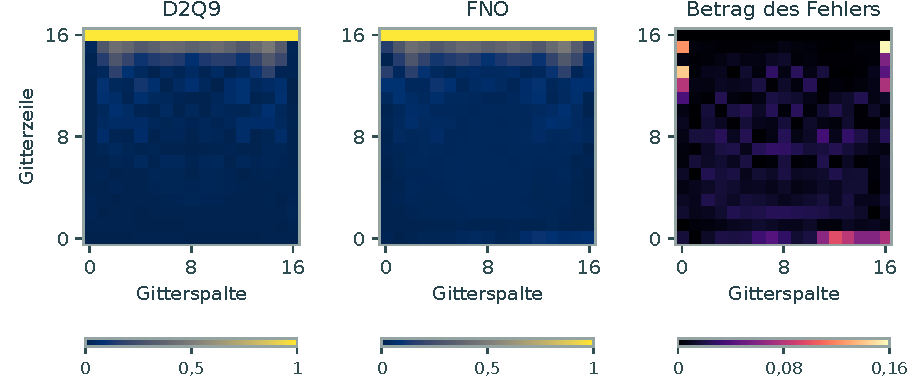
\includegraphics[width=.88\linewidth,height=49mm,keepaspectratio]{cp2kavitaet.pdf}\par}\capline{Der bewegte Deckel setzt das Innere der Kavität in Bewegung.}
\seite{}{Lattice-Boltzmann}\anchorpage{2}{abs8-1}{8.1 · Von der kinetischen Beschreibung zur Strömung}\ey{ABSCHNITT 8.1}\ptitle{Von der kinetischen Beschreibung zur Strömung}
\hypertarget{punkt8-1-1}{}\subt{8.1.1\enspace Verteilungen über Geschwindigkeiten}
Stellen Sie sich eine kleine Messzelle vor. Zwei Teilchenpakete können gleich viel Masse enthalten und doch mit sehr verschiedenen Geschwindigkeiten eintreffen. Die Verteilung \(f(x,\xi,t)\) beschreibt, wie viel Masse am Ort \(x\) einer Geschwindigkeit \(\xi\) zugeordnet ist. Ohne äußere Kraft lautet ihre Transportgleichung \(\partial_t f+\xi\cdot\nabla_x f=\Omega(f)\). Freier Transport verschiebt die Verteilung, Stöße verändern ihre Form.
\hypertarget{punkt8-1-2}{}\subt{8.1.2\enspace BGK-Relaxation und hydrodynamische Grenze}
BGK ersetzt den komplizierten Stoßoperator durch \(-(f-f^{eq})/\tau_{phys}\). Kleines positives \(\tau_{phys}\) führt rasch zum örtlichen Gleichgewicht. Dichte und Impuls sind die niedrigsten Momente. Unter geeigneter Skalierung, kleinen Knudsen- und Mach-Zahlen und hinreichender Gitterisotropie liefern ihre Bilanzen die makroskopische Strömungsdynamik. Der folgende Gitteralgorithmus benutzt eine dimensionslose Relaxationszeit in Schritten.
\seite{}{Lattice-Boltzmann}\anchorpage{2}{abs8-2}{8.2 · Das D2Q9-Gittermodell}\ey{ABSCHNITT 8.2}\ptitle{Das D2Q9-Gittermodell}
\hypertarget{punkt8-2-1}{}\subt{8.2.1\enspace Neun Richtungen und ihre Gewichte}
In der Mitte bleibt ein Anteil liegen, vier ziehen längs der Achsen, vier diagonal. Die Gewichte betragen \(4/9,1/9,1/36\) je Richtung der jeweiligen Gruppe. Ihre Summe ist eins. Gegenrichtungen wie Ost und West heben sich im ersten Moment eines ruhenden Gleichgewichts auf. In Gittereinheiten gilt \(c_s^2=1/3\).
\hypertarget{punkt8-2-2}{}\subt{8.2.2\enspace Das diskrete Gleichgewicht bei kleiner Mach-Zahl}
Eine Entwicklung der Maxwell-Verteilung bis zum Quadrat in \(u\) liefert
\[
 f_i^{eq}=w_i\rho\left(1+\frac{c_i\cdot u}{c_s^2}
 +\frac{(c_i\cdot u)^2}{2c_s^4}-\frac{u\cdot u}{2c_s^2}\right).
\]
Dreht sich das Fluid nach Osten, wächst die ostwärts gerichtete Population relativ zur westwärts gerichteten. Die quadratischen Terme sorgen für das passende zweite Moment im Arbeitsbereich der Näherung.
\hypertarget{punkt8-2-3}{}\subt{8.2.3\enspace Dichte, Impulsdichte und Impulsfluss}
Ohne äußere Kraft gilt \(\rho=\sum_i f_i\) und \(\rho u=\sum_i c_i f_i\). Der Impulsfluss ist der Tensor \(\Pi=\sum_i(c_i\otimes c_i)f_i\). Schon die Einheiten unterscheiden Masse pro Volumen, Impuls pro Volumen und Impulstransport über eine Fläche. Im Labor ändern wir die Populationen bei unveränderten ersten beiden Momenten.
\lektion{Neun Zahlen in einer einzigen Zelle}{zellenlbm}{Rechenversuch}{Lattice-Boltzmann}
\lernziel{Sie können vorhersagen, wie eine Lattice-Boltzmann-Zelle auf eine kleine Störung reagiert und was die Nachbarzelle im nächsten Schritt erhält.}
Die Einträge \(f_i\) verteilen die lokale Dichte auf mögliche Bewegungsrichtungen. Für Flüssigkeit in Ruhe bei \(\rho=1\) hat der D2Q9-Gleichgewichtszustand in Gittereinheiten die folgenden Werte.
{\tblstart\begin{tabularx}{\linewidth}{@{}Yrr@{}}\toprule
\hd{Richtung}&\hd{Anzahl}&\hd{Wert je Richtung}\\\midrule
Ruhe, \(\mathbf c=(0,0)\)&1&4/9\\
Ost, Nord, West, Süd&4&1/9\\
Diagonalen&4&1/36\\\bottomrule
\end{tabularx}\par}
Die Dichte ist \(4/9+4/9+4/36=1\). Gegenüberliegende Richtungen haben gleiches Gewicht. Ihre Impulse heben sich auf, also ist die mittlere Geschwindigkeit null. In einer gleichmäßig ruhenden Flüssigkeit wiederholt sich dieser Zustand nach Kollision und Transport.
\subt{Ein Schritt außerhalb des Gleichgewichts}
Geben Sie Ost und West je \(0{,}02\) zusätzlich und nehmen Sie dem Ruheanteil \(0{,}04\) weg. Dichte und Impuls bleiben gleich. Trotzdem hat sich der Zustand geändert. Wählen wir für die Handrechnung \(\omega=1/2\), halbiert die BGK-Kollision jede Abweichung vom Gleichgewicht. Der Ostanteil geht von \(1/9+0{,}02=0{,}131111\ldots\) auf \(1/9+0{,}01=0{,}121111\ldots\) zurück. Der Ruheanteil bleibt um \(0{,}02\) unter \(4/9\).

Beim anschließenden Transport wandert der neue Ostanteil in die östliche Nachbarzelle. Dort muss seine Dichtewirkung mit den acht anderen ankommenden oder ruhenden Anteilen zusammengezählt werden. Erst daraus lässt sich eine Geschwindigkeit an diesem Ort bestimmen. Am Deckel greift zusätzlich die vorgeschriebene Randregel.
\notebox{Probe}{Welchen Unterschied hätte eine einzige gespeicherte Geschwindigkeit vor der Kollision gezeigt? Beide Zustände haben Geschwindigkeit null. Die neun gespeicherten Anteile bewahren zusätzlich das Richtungsungleichgewicht.}
\srcs{\href{https://benchpress.readthedocs.io/autodoc_benchmarks/lattice_boltzmann_D2Q9.html}{D2Q9-Gewichte im Rechenbeispiel von Jonas Latt} · \texttt{python methodenlabor.py} · \see{schluss13}{Lokaler Erhaltungsbeweis}.}

\seite{}{Lattice-Boltzmann}\anchorpage{2}{abs8-3}{8.3 · Kollision und Streaming}\ey{ABSCHNITT 8.3}\ptitle{Kollision und Streaming}
\hypertarget{punkt8-3-1}{}\subt{8.3.1\enspace Lokale Kollision}
Alle neun Eingangswerte stammen aus der gleichen Zelle. Nach der Momentenbildung berechnet man \(f_i^*=f_i-(f_i-f_i^{eq})/\tau\). Für \(\tau=2\) halbiert die Kollision jede Abweichung vom aktuellen Gleichgewicht. Die Ausgangswerte gehören weiter zur selben Zelle.
\hypertarget{punkt8-3-2}{}\subt{8.3.2\enspace Transport in den Nachbarpuffer}
Mit Gitterzeit eins schreibt Streaming \(f_i(x+c_i,t+1)=f_i^*(x,t)\). Eine doppelte Pufferung verhindert, dass ein frisch geschriebener Wert im selben Takt ein zweites Mal reist. Gegenprobe mit einem einzigen markierten Ostanteil: Nach einem Takt muss der Wert genau eine Spalte weiter im Ostkanal erscheinen.
\hypertarget{punkt8-3-3}{}\subt{8.3.3\enspace Beweis der lokalen Erhaltung}
Die D2Q9-Symmetrien liefern \(\sum w_i=1,\ \sum w_ic_i=0,\ \sum w_ic_ic_i^T=c_s^2I\), und alle ungeraden dritten Momente verschwinden. Einsetzen in das Gleichgewicht ergibt \(\sum f_i^{eq}=\rho\) und \(\sum c_if_i^{eq}=\rho u\). Daher haben die Kollisionskorrekturen sowohl Summe als auch erstes Moment null. Beim Streaming wandert Masse zwischen den Zellen. Eine periodische Gesamtbilanz bleibt erhalten, eine bewegte Wand kann Impuls zuführen.
\seite{}{Lattice-Boltzmann}\anchorpage{2}{abs8-4}{8.4 · Wände und Einheiten}\ey{ABSCHNITT 8.4}\ptitle{Wände und Einheiten}
\hypertarget{punkt8-4-1}{}\subt{8.4.1\enspace Bounce-back an einer ruhenden Wand}
Eine Population, die im nächsten Schritt in eine feste Wand liefe, kehrt in die Gegenrichtung zurück. Vollweg- und Halbweg-Varianten verorten die Rückgabe unterschiedlich. Damit ändern sich die effektive Wandlage und möglicherweise die Konvergenz. Die Lage des geometrischen Randes gehört deshalb zum Vergleich zweier Gitter.
\hypertarget{punkt8-4-2}{}\subt{8.4.2\enspace Geschwindigkeitsrand und bewegter Deckel}
Bei Zou–He werden fehlende einlaufende Populationen aus den Zielmomenten und einer Schließungsannahme für den Nichtgleichgewichtsanteil rekonstruiert. Nach diesem Update müssen Normalmassenstrom und gewünschte Tangentialgeschwindigkeit zusammenpassen. CP2 benutzt im hier reproduzierten Algorithmus Vollweg-Reflexion an ruhenden Wänden und vorgegebene Gleichgewichtspopulationen an der Deckelzeile. Ein Wechsel der Randvorschrift ist ein neuer Versuch.
\hypertarget{punkt8-4-3}{}\subt{8.4.3\enspace Physikalische und Gittereinheiten}
Bei Gitterweite \(\Delta x\) und Zeittakt \(\Delta t\) gilt \(u_{lat}=u_{phys}\Delta t/\Delta x\), \(\nu_{lat}=\nu_{phys}\Delta t/\Delta x^2=c_s^2(\tau-1/2)\). Die Reynolds-Zahl \(UL/\nu\) bleibt unter konsistenter Umrechnung gleich. Positive BGK-Viskosität erfordert \(\tau>1/2\). Für einen belastbaren Lauf prüfen wir außerdem Mach-Zahl, Massenbilanz und die Mittellinienprofile.
\srcs{\href{https://arxiv.org/abs/comp-gas/9611001}{Zou und He, Geschwindigkeits- und Druckränder} · \see{pylbm}{CP2-Kavität}.}
\lektion{Eine D2Q9-Zelle Schritt für Schritt}{alg8}{Werkstatt}{Kapitel 8}
Zwei Gitterpuffer trennen ankommende Populationen von gerade fortgeschriebenen. Beim Streaming muss eine nach Osten auslaufende Population der westlichen Nachbarzelle im Ostkanal der Zielzelle erscheinen.
{\small\begin{verbatim}
fuer jede Zelle x:
    rho = summe(f[x])
    u = impuls(f[x]) / rho
    fuer jede Richtung i:
        eq = gleichgewicht(i, rho, u)
        stern[x,i] = f[x,i] - (f[x,i] - eq) / tau
fuer jede fluide Verbindung (x, i):
    neu[x + c[i], i] = stern[x, i]
behandle_Wandverbindungen_nach_der_Randregel()
\end{verbatim}}
\subt{Selbst rechnen}
Ein ruhendes Gitter besitzt je Zelle Dichte eins. Ost und West erhalten jeweils 0,02 zusätzlich, vom Ruheanteil werden 0,04 abgezogen. Wie sieht die Störung nach einer BGK-Kollision bei \(\tau=2\) aus?
\notebox{Lösung}{Dichte und Impuls bleiben unverändert. Dadurch bleibt auch das Gleichgewicht gleich. Der Kollisionsschritt halbiert jede Abweichung, also +0,01 im Ost- und Westkanal und \ensuremath{-}0,02 im Ruhekanal. Erst das Streaming verteilt diese Störung auf Nachbarn.}

\seite{}{Scientific Machine Learning}\anchorpage{1}{neu9}{9 · Scientific Machine Learning und Operator Learning}\ey{KAPITEL 9}\ptitle{Scientific Machine Learning und Operator Learning}
Eine Saite wird heute in ihrer Mitte, morgen ein Stück weiter links gezupft. Für jede Anfangsform kann ein klassischer Solver die ganze Bewegung erneut berechnen. Könnte ein Netz stattdessen die Abbildung von einer vollständigen Anfangsform zur späteren Form lernen? Eine Messung in der Mitte genügt zur Antwort nicht. Sie übersieht jeden Fehler, der sich dort gerade aufhebt.
\subt{Der Weg durch das Kapitel}
{\tblstart\begin{tabularx}{\linewidth}{@{}Yr@{}}\toprule
\hyperlink{abs9-1}{9.1 · Surrogate, Residuen und Operatoren} & \pagelink{abs9-1}\\[2pt]
\hyperlink{abs9-2}{9.2 · Eine Fourier-Neural-Operator-Schicht} & \pagelink{abs9-2}\\[2pt]
\hyperlink{abs9-3}{9.3 · Physikalischer Basissolver und gelernte Korrektur} & \pagelink{abs9-3}\\[2pt]
\bottomrule\end{tabularx}\par}
\par\vfill{\centering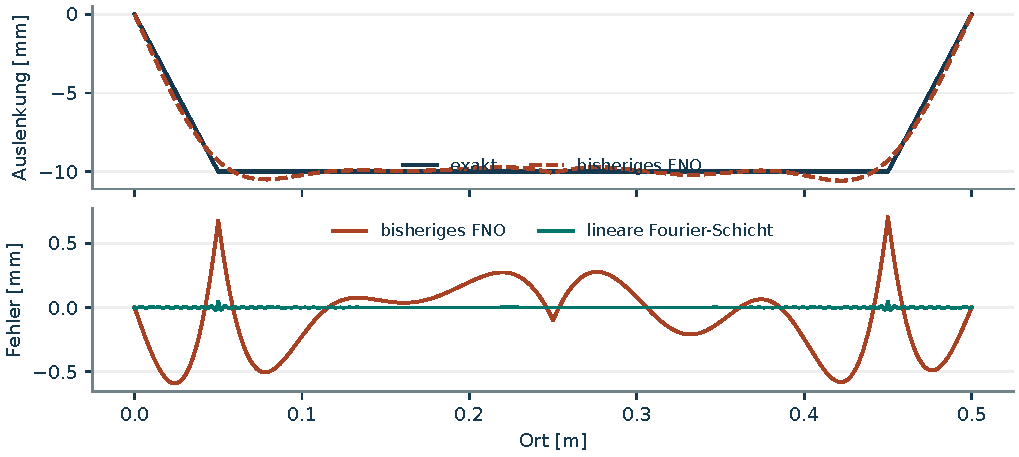
\includegraphics[width=.88\linewidth,height=49mm,keepaspectratio]{fno_saite_feld.pdf}\par}\capline{Das örtliche Fehlerprofil unterscheidet Modelle, die an einem Messpunkt fast übereinstimmen.}
\seite{}{Scientific Machine Learning}\anchorpage{2}{abs9-1}{9.1 · Surrogate, Residuen und Operatoren}\ey{ABSCHNITT 9.1}\ptitle{Surrogate, Residuen und Operatoren}
\hypertarget{punkt9-1-1}{}\subt{9.1.1\enspace Was bildet das Modell ab?}
Ein gewöhnliches Surrogat kann etwa die maximale Auslenkung aus einer einzigen Zugposition schätzen. Bei einer Feldvorhersage sind Eingabe und Ausgabe dagegen ganze Funktionen. Die Messorte, die Norm und die Verteilung der Trainingseingaben legen fest, welche Unterschiede im Lernverfahren überhaupt sichtbar werden.
\hypertarget{punkt9-1-2}{}\subt{9.1.2\enspace Physikalisch informierte neuronale Netze}
Ein PINN setzt eine differenzierbare Netzfunktion in die Differentialgleichung ein. Der Verlust kombiniert PDE-Residuen an Kollokationspunkten mit Anfangs-, Rand- und gegebenenfalls Messfehlern. Eine nahezu konstante falsche Lösung der Wärmegleichung kann einen kleinen inneren Defekt haben, während sie die Randwerte verfehlt. Auch starke Gewichtung einzelner Terme ersetzt keine unabhängige Prüfung zwischen Messpunkten.
\hypertarget{punkt9-1-3}{}\subt{9.1.3\enspace DeepONet und FNO}
Ein DeepONet verknüpft typischerweise Merkmale der Eingabefunktion aus einem Zweignetz mit Ortsmerkmalen eines zweiten Netzes. Ein FNO mischt räumliche Information über spektrale Operatoren. Beide approximieren eine Abbildung zwischen Funktionenräumen auf endlich vielen Beispielen. Ein Test auf neuen Eingabefamilien verlangt eine eigene Stichprobe.
\lektion{Wie lernt ein einzelnes Neuron?}{nnrechnen}{Einstieg}{Neuronale Netze}
\lernziel{Sie können eine Vorhersage, einen Fehler und eine Gewichtsänderung selbst berechnen.}
Stellen Sie sich einen normierten Sensor vor. Für den Eingang \(x=2\) wurde als Ziel \(y=1\) gemessen. Ein künstliches Neuron bildet eine gewichtete Summe und wendet eine Funktion darauf an. Wir verwenden \(\hat y=\max(0,wx)\). Die Funktion \(\max(0,z)\) heißt \emph{ReLU}. Zur ersten Handrechnung setzen wir die sonst häufig verwendete additive Verschiebung auf null.
\subt{Vorhersagen und bewerten}
Wir starten bei \(w=1\). Die Vorhersage ist \(\hat y=2\). Als Verlust dient die Hälfte des quadratischen Fehlers \(L(w)=\tfrac12(\hat y-y)^2\), hier also \(0{,}5\). Der Verlust misst an diesem Trainingsbeispiel, wie gut das Gewicht passt.
\subt{Ein Schritt, der den Verlust verkleinert}
Auf dem positiven Ast der ReLU ist \(\hat y=wx\). Nach der Kettenregel ist \(L'(w)=(wx-y)x=2\). Mit Lernrate \(\eta=0{,}1\) geht der Gradientenabstieg entgegen der positiven Ableitung:
\[
 w_{\rm neu}=w-\eta L'(w)=0{,}8,\qquad
 \hat y_{\rm neu}=1{,}6,\qquad L(w_{\rm neu})=0{,}18 .
\]
Ein Netz verknüpft viele solcher Einheiten zu Schichten. Beim Training werden die Ableitungen mit der Kettenregel von der Ausgabe zurück zu den Gewichten gerechnet (Backpropagation). In der Vorhersage bleiben die gewählten Gewichte fest. Ob das Modell für andere Eingaben taugt, wird an zurückgehaltenen Beispielen geprüft.
\notebox{Eine eigene Gegenprobe}{Bei \(x=-2\) wäre für die Regel \(y=x/2\) das Ziel \(-1\). Die ReLU am Ausgang kann nur Werte ab null liefern. Für eine schwingende Saite muss die Netzausgabe beide Vorzeichen zulassen. Für den Betrag einer Strömungsgeschwindigkeit passt eine nichtnegative Ausgabe.}
\srcs{\texttt{python methodenlabor.py} · \see{pyfno}{Von einzelnen Zahlen zu ganzen Feldern} · \see{netzarten}{Drei Arten, Physik und Lernen zu verbinden}.}

\lektion{PINN, DeepONet oder Fourier-Operator?}{netzarten}{Methodenwahl}{Neuronale Verfahren}
Bei der Saite kann man zwei verschiedene Fragen stellen. Wie schwingt \emph{diese} Anfangsform? Wie ändern sich die späteren Profile, wenn wir die Anfangsform austauschen? Der Auftrag bestimmt die Eingaben eines Netzes und die Information, aus der es lernt.
\subt{Ein physikinformiertes Netz für eine feste Saite}
Ein Physics-Informed Neural Network (PINN) bekommt hier Ort und Zeit und gibt \(u_\theta(x,t)\) aus. Wir bewerten an ausgewählten Punkten den Gleichungsrest \(r=u_{\theta,tt}-c^2u_{\theta,xx}\). Automatische Differentiation leitet dafür die im Netz ausgeführten Operationen ab. In den Verlust gehen außerdem die Fehler bei Anfangsauslenkung, Anfangsgeschwindigkeit und Randwerten ein. Die Nullfunktion hat überall Rest null und erfüllt die festen Ränder. Für eine ausgelenkte Saite verfehlt sie die Anfangsform. Dieser Gegenversuch erklärt, warum die einzelnen Verlustanteile nötig sind.
\subt{DeepONet lernt aus einer Familie von Anfangsformen}
Ein Teilnetz liest Messwerte der Eingabefunktion \(g\) an festgelegten Sensororten und liefert Koeffizienten \(b_k(g)\). Ein zweites Teilnetz liest den abzufragenden Ort und die Zeit und liefert Basiswerte \(t_k(x,t)\). Ihre Summe von Produkten \(\sum_k b_k(g)t_k(x,t)\) gibt die Vorhersage. Für die Familie \(g(x)=a\sin(\pi x/L)\) genügt ein Produkt bereits exakt: Der Mittensensor liefert \(a\), der zweite Faktor ist \(\sin(\pi x/L)\cos(\pi ct/L)\). Gegenaufgabe bei \(t=0\): Vergleichen Sie \(g_1=0\) mit \(g_2=a\sin(2\pi x/L)\), \(a\ne0\). Am Mittensensor liefern beide null. Bei \(L/4\) liefern sie 0 bzw. \(a\). Gleiche Sensoreingaben können daher verschiedene Ausgaben verlangen.
\subt{FNO liefert im CP2-Versuch ganze Gitterprofile}
Unser FNO bekommt das Eingabefeld auf dem Gitter. Es mischt räumliche Frequenzen und lokale Merkmale. Die Trainingsziele stammen für die Saite aus der Modenlösung und für die Kavität aus dem D2Q9-Code. PINN und DeepONet sind hier Entwurfsalternativen. Die gemessenen CP2-Netzfehler gelten für das tatsächlich trainierte FNO.
\srcs{\href{https://doi.org/10.1016/j.jcp.2018.10.045}{Raissi u.\,a. (2019), PINNs} · \href{https://www.nature.com/articles/s42256-021-00302-5}{Lu u.\,a. (2021), DeepONet} · \see{pyvergleich}{Gemessene FNO-Fehler}.}

\seite{}{Scientific Machine Learning}\anchorpage{2}{abs9-2}{9.2 · Eine Fourier-Neural-Operator-Schicht}\ey{ABSCHNITT 9.2}\ptitle{Eine Fourier-Neural-Operator-Schicht}
\hypertarget{punkt9-2-1}{}\subt{9.2.1\enspace Eine Faltung über das ganze Feld}
Für einen translationsinvarianten Kern \(k(x-y)\) ist die Faltung \(\int k(x-y)v(y)\,dy\) im periodischen Fall im Fourierraum eine Multiplikation. Eine tiefe Operatorarchitektur lernt diesen globalen Anteil und kann über einen lokalen Term und Nichtlinearitäten komplexere Abbildungen darstellen.
\hypertarget{punkt9-2-2}{}\subt{9.2.2\enspace Von der FFT zurück in den Ortsraum}
Eine Schicht berechnet \(v^+=\sigma(Wv+b+\mathcal F^{-1}(R_k\widehat v_k))\). Zuerst transformiert die FFT jeden Eingangskanal. Für die behaltenen Moden mischt die komplexe Matrix \(R_k\) die Kanäle. Andere Moden des spektralen Zweigs werden auf null gesetzt. Nach der inversen FFT addiert man die punktweise affine Abbildung. Für ein reelles Feld müssen die Fourierkoeffizienten die konjugierte Symmetrie erfüllen. Zeichnen Sie die zwei parallelen Wege und markieren Sie den einzigen Schritt, der über alle Orte koppelt.
\hypertarget{punkt9-2-3}{}\subt{9.2.3\enspace Übertragung auf ein feineres Gitter}
Dieselben Gewichte können auf kompatiblen Gittern dieselben physikalischen Moden ansprechen. Dafür müssen Intervall, Randbehandlung, Normierung und Modenzuordnung passen. Ein auf einem groben Gitter unaufgelöster Knick bleibt eine Herausforderung. Der Test vergleicht dieselbe Eingangsfunktion auf zwei Gittern gegen eine unabhängige Lösung und nennt für jedes Gitter den Feldfehler.
\srcs{\href{https://arxiv.org/abs/2010.08895}{Li und andere, Fourier Neural Operator} · \see{fnotransfer}{CP2-Gitterwechsel}.}
\lektion{Was lernt ein neuronaler Operator?}{pyfno}{Verfahren}{Neuronale Operatoren}
Ein gewöhnliches künstliches Neuron bildet Eingaben \(z_j\) auf \(a=\sigma(b+\sum_j w_j z_j)\) ab. Die Gewichte \(w_j\) und der Versatz \(b\) werden gelernt. \(\sigma\) ist eine vorgegebene, gewöhnlich nichtlineare Aktivierungsfunktion. Ein \emph{Operator} ordnet hier einer ganzen Eingabefunktion eine oder mehrere Ausgabefunktionen zu. An einem Gitter sehen wir diese Funktionen als Zahlenfelder.
\subt{Eine Schicht des Fourier Neural Operator}
Ein FNO zerlegt seine internen Felder mit einer diskreten Fouriertransformation in räumliche Frequenzen. Für ausgewählte Frequenzen mischt er die Merkmale mit lernbaren Matrizen. Nach der Rücktransformation addiert er einen lokalen Beitrag und wendet eine Aktivierung an. Aus mehreren solchen Schichten entsteht in der Saite die Abbildung \(g(\cdot)\mapsto (u(\cdot,5),u(\cdot,8))\). Die analytische Kontrollrechnung verwendet bekannte Wellengesetze; die Matrizen des Netzes werden an Beispielen bestimmt.
\subt{Woher kommen richtige Trainingsantworten?}
Für die Saite ziehen wir unabhängige Anfangsprofile aus acht Sinusmoden. Die \(k\)-te Mode wird mit \(\cos(k\pi ct/L)\) multipliziert. Für die Kavität variieren wir die anfängliche Dichte sanft um eins, bei ruhender Flüssigkeit und gleichem Deckel. Für jedes Eingabefeld erzeugt D2Q9 das Ziel \(|\mathbf u|/u_\mathrm{Deckel}\). Ein Betrag am Netzausgang erzwingt nichtnegative Vorhersagen. Bei der Saite erzwingt eine ungerade Projektion verschwindende Randwerte.
\subt{Welche Daten darf das Netz sehen?}
Je Fall dienen 96 ganze Felder zum Optimieren der Gewichte. Nach jeder Epoche bewerten wir 16 weitere Felder und speichern die besten Gewichte. Erst danach werten wir 24 andere Felder aus. Bei der Saite kommen Dreiecksform und feineres Gitter als zusätzlicher Transfer hinzu, bei der Kavität der gleichförmige Ruhezustand. Eine Aufteilung einzelner Gitterpunkte derselben Trajektorie könnte dasselbe Experiment in beiden Mengen erscheinen lassen.
\srcs{\href{https://github.com/neuraloperator/neuraloperator}{NeuralOperator, Python-Paket neuraloperator} · \href{https://openreview.net/pdf?id=c8P9NQVtmnO}{Li u.\,a. (2021), Fourier Neural Operator} · \cpcode{argesim_benchmarks/experiments/cp2_fields.py}{Erzeugung der Referenzfelder}.}

\lektion{Saite · Wie lernt eine Fourier-Schicht?}{fnosaite}{Labor}{CP2 · Saite}
Denken Sie sich die gezupfte Saite aus einfachen Schwingungsformen zusammengesetzt. Die \(k\)-te Form \(\sin(k\pi x/L)\) verschwindet an beiden Enden. Bei einer idealen linearen Saite bleibt jede Form für sich erhalten; nur ihre Amplitude ändert sich. Ein trainierbarer Faktor \(m_k(t)\) pro Mode genügt daher. Wie groß er sein soll, lernt die Fourier-Schicht aus Paaren von Eingangs- und Ausgangsamplituden.
\[
 \widehat m_k(t_i)=
 \frac{\sum_j a_{jk}(0)\,a_{jk}(t_i)}{\sum_j a_{jk}(0)^2}.
\]
Mit angeregter Mode folgt die Formel aus der Ableitung der Fehlerquadratsumme. Die 96 Profile liefern Faktoren für 192 Moden und 321 Zeiten von 0 bis 8 s. Dazwischen interpolieren wir linear. Für die Referenz gilt \(m_k(t)=\cos(ck\pi t/L)\). Setzt man \(a_{jk}(t_i)=a_{jk}(0)\cos(\omega_kt_i)\) ein, kürzt sich die Summe der Quadrate. Im Kontrolllauf ersetzen wir nur die Faktoren durch diesen Kosinus, bei gleicher Modenzahl und Interpolation. Die Sinustransformation entspricht der Fourier-Transformation der ungeraden Fortsetzung.
\minifig{fno_saite_feld}{59mm}{Mittig gezupfte Saite auf 501 Knoten. Oben stehen die Profile für 5 und 8 s, unten die lokalen Fehler auf derselben Millimeterskala. Das ursprüngliche FNO glättet die Knicke.}
\subt{Der Vergleich am selben Dreieck}
Nach 5 s fällt der relative Fehler von \(3{,}0009\,\%\) auf \(0{,}04303\,\%\), nach 8 s von \(0{,}8816\,\%\) auf \(0{,}01416\,\%\). Die analytische Kontrollschicht erzielt ebenfalls \(0{,}04303\,\%\) und \(0{,}01416\,\%\). Ihr größter Profilabstand zur gelernten Schicht liegt unter \(5\cdot10^{-14}\unitm m\). Der neue absolute RMS beträgt \(4{,}00\) bzw. \(4{,}05\,\mu\mathrm m\). Newmark erreicht \(0{,}3745\) bzw. \(0{,}1519\,\%\), Störmer--Verlet \(0{,}2313\) bzw. \(0{,}0946\,\%\) bei den Einstellungen der vorangehenden Studie.
\srcs{Eine Auswertung derselben Gewichte mit \href{https://neuraloperator.github.io/dev/modules/generated/neuralop.layers.spectral_convolution.SpectralConv.html}{NeuralOperator · SpectralConv} unterscheidet sich hier um höchstens \(1{,}23\cdot10^{-8}\unitm m\) von der Sinusauswertung.}

\lektion{Welche Fehlergrenze lässt sich beweisen?}{fnobeweis}{Vertiefung}{CP2 · Operatortheorie}
Schreiben wir die Anfangsform in einer orthonormalen Sinusbasis als \(g=\sum_k a_k e_k\). Orthogonalität bedeutet hier \(\|g\|_2^2=\sum_k |a_k|^2\). Eine präzise Annahme an die Glattheit lautet \(\sum k^{2s}|a_k|^2\le R^2\), \(s>0\). Große \(s\) begrenzen die Energie schneller räumlicher Wechsel stärker.
\subt{Satz für die trainierte lineare Schicht}
Seien \(K\) die behaltenen Moden, \(\omega_k=ck\pi/L\), \(d\) der größte Abstand zweier Zeitstützstellen und \(\epsilon\) der größte Fehler eines gespeicherten Faktors an einer Stützstelle. Für \(0\le t\le8\) gilt
\[
 \|(\widehat S(t)-S(t))g\|_2 \le R\max\!\left\{
 \max_{1\le k\le K}\frac{\epsilon+\omega_k^2d^2/8}{k^s},
 (K+1)^{-s}\right\}.
\]
\proofpart{Der Fehler linearer Interpolation einer zweimal differenzierbaren Funktion ist höchstens \(d^2\max|m''|/8\). Für den Kosinus ist \(\max|m_k''|\le\omega_k^2\); ein konvexes Mittel zweier Stützfehler hat Betrag höchstens \(\epsilon\). Ab Mode \(K+1\) ist der Betrag des ausgelassenen Multiplikators höchstens eins. Quadrieren, in der orthonormalen Basis summieren und den größten gewichteten Faktor ausklammern liefert die Behauptung.}
Eine Intervallauswertung aller 61\,632 gespeicherten Faktoren ergibt \(\epsilon<1{,}36\cdot10^{-13}\). An den Stützzeiten entfällt der Interpolationsterm. Auf einem festen Gitter gilt die Rechnung für dessen diskrete Sinuskoeffizienten mit \(K\le N-2\). Bei einer abgetasteten kontinuierlichen Form kommt der Fehler ihrer räumlichen Darstellung hinzu. Die Gitterstudie misst ihn mit.
\subt{Was lässt sich über das frühere mehrschichtige FNO sagen?}
Für das frühere Netz liefert die Verkettung von Schichtnormen \(\|F(g)-F(h)\|_2\le24\,217\|g-h\|_2\). Jede Fourier-Matrix wird durch ihre Frobeniusnorm beschränkt, die GELU-Ableitung durch \(1{,}13\); bei parallelen Zweigen addieren sich Grenzen. Ungerade Projektion macht \(F(0)=0\). Für jede einzelne Ausgabe und eine diskrete Eingabekugel mit Radius \(R\) folgt so \(24\,218R\) als konservative absolute Fehlergrenze. Die genauere modale Schranke oben nutzt wesentlich mehr Modellstruktur.
\srcs{\texttt{scripts/cp2\_accuracy/operator\_bounds.py} prüft die festen binären Gewichte als reelle Koeffizienten mit nach außen gerundeter Intervallarithmetik. Die Laufzeitrundung einer GPU ist eine eigene Fehlerquelle.}

\seite{}{Scientific Machine Learning}\anchorpage{2}{abs9-3}{9.3 · Physikalischer Basissolver und gelernte Korrektur}\ey{ABSCHNITT 9.3}\ptitle{Physikalischer Basissolver und gelernte Korrektur}
\hypertarget{punkt9-3-1}{}\subt{9.3.1\enspace Welchen Anteil übernimmt das Netz?}
Für eine grobe Vorhersage \(B(a)\) und eine feine Referenz \(G(a)\) kann das Lernziel \(G(a)-B(a)\) sein. Dann ergibt sich \(\hat G=B+N_\theta\). Ein sauberes Experiment enthält den unveränderten Basissolver, eine analytische Korrektur, soweit vorhanden, und die Netzkorrektur auf identischen Testfeldern. So wird bei der Saite sichtbar, was bereits die Modenwahl und die Randfortsetzung leisten.
\hypertarget{punkt9-3-2}{}\subt{9.3.2\enspace Fehlertransport und Verallgemeinerung}
Wird ein gelernter Einzelschritt immer wieder eingesetzt, kann sich ein Defekt \(\delta\) unter einer Lipschitz-Schranke \(K\) zu \(\|e_n\|\le K^n\|e_0\|+\delta\sum_{j=0}^{n-1}K^j\) aufsummieren. Eine direkte Vorhersage zu einem festen Endzeitpunkt hat einen anderen Fehlerweg. In CP2 prüfen gespiegelte Zupfstellen die Symmetrie. Eine neue Reynolds-Zahl der Kavität prüft dagegen den Transfer auf einen anderen Betriebspunkt.
\notebox{Gegenprobe}{Teilen Sie die Testdaten nach physikalischer Eingabefamilie. Werden Nachbarn derselben Trajektorie auf Training und Test verteilt, beantwortet der gemessene Fehler eine wesentlich leichtere Frage.}
\lektion{Was ist beim Methodenvergleich noch offen?}{forschungsmethoden}{Forschung}{Methodenvergleich · November 2026}
\subt{Klassische Diskretisierung und Lattice-Boltzmann}
Am Transportbeispiel lassen sich Erhaltung, Positivität und Genauigkeit einzeln testen. Für die CP2-Saite ist die Schrittgrenze der expliziten Diskretisierung herleitbar. Der Gitterversuch für die Fourier-Schicht vergleicht die geknickte Saite bereits an \(6\cdot4\cdot99=2\,376\) Kombinationen aus Zupfposition, Gitter und Zeit (S.\,\pagelink{fnoabl}). Offen bleibt das genaue kontinuierliche Maximum des absoluten RMS-Fehlers für diese Dreiecke auf \([0,8]\unitm s\). Die Schranke auf S.\,\pagelink{fnobeweis} gilt unter ihren dort angegebenen Regularitätsannahmen.

Eine Untersuchung von LBM-Randregeln aus dem Jahr 2024 vergleicht Varianten an laminaren Strömungen mit bekannten Referenzen. Das ist für CP2 wichtig, weil unser Deckel seine Geschwindigkeit vorschreibt. Für die stationäre Kavität publizierten Ghia, Ghia und Shin Vergleichsdaten. Der \see{fnolang}{vollständige Kavitätslauf} prüft inzwischen beide Geschwindigkeitskomponenten, die Annäherung an den stationären Zustand und drei Gitterweiten.
\subt{Was zeigt die Forschung zu gelernten Operatoren?}
Herde u.\,a. untersuchten 2024 mit Poseidon ein vortrainiertes Modell an 15 nachgelagerten PDE-Aufgaben. Park u.\,a. verglichen 2026 in einem Preprint kurze und lange Vorhersagefolgen mehrerer Modelle. In ihrer Untersuchung wuchs der Fehler bei vielen längeren Folgen. Beide Studien betreffen andere Daten und Architekturen als unser CP2-Praktikum.
\subt{Wie groß ist der Gewinn auf unabhängigen Daten?}
Die anschließende Studie prüft sechs Zupfpositionen, absolute und relative Fehler sowie veränderte Deckelgeschwindigkeiten, Zeitschritte und Gitter. Zwei Rechnungen zeigen, welcher Anteil der Verbesserung von der Modellstruktur und welcher vom neuronalen Anteil stammt. Eine bewiesene Fehlergrenze nutzt die lineare Wellengleichung.
\srcs{\href{https://doi.org/10.1016/j.camwa.2024.08.009}{LBM-Randbedingungen (2024)} · \href{https://doi.org/10.1016/0021-9991(82)90058-4}{Ghia u.\,a. (1982)} · \href{https://proceedings.nips.cc/paper_files/paper/2024/hash/84e1b1ec17bb11c57234e96433022a9a-Abstract-Conference.html}{Herde u.\,a. (NeurIPS 2024)} · \href{https://arxiv.org/abs/2610.31935}{Park u.\,a. (Preprint, Oktober 2026)}.}

\lektion{Eine Spektralschicht ohne verdeckte Achsen}{alg9}{Werkstatt}{Kapitel 9}
Wir nehmen ein reelles Eingangsfeld mit einer Kanalachse und einer räumlichen Achse. Für diesen Lehrschritt ist die Länge N fest, und K überschreitet die Zahl der verfügbaren reellen FFT-Moden nicht. Randfortsetzung und Normierung müssen schon zur Datenerzeugung passen.
{\small\begin{verbatim}
v_hat = rfft(v, axis=Ort)
z_hat = komplexe_Nullen(Ausgabekanaele, N//2 + 1)
fuer k in den ersten K Moden:
    z_hat[:,k] = R[k] @ v_hat[:,k]
spektral = irfft(z_hat, n=N, axis=Ort)
v_neu = Aktivierung(spektral + W @ v + bias)
\end{verbatim}}
\subt{Selbst rechnen}
Ein Eingang enthält nur eine Mode oberhalb der behaltenen K Moden. Was kann dieser einzelne lineare spektrale Pfad übertragen?
\notebox{Lösung}{In diesem Pfad ist die Ausgabe null. Der lokale Pfad W kann den Eingang trotzdem weiterreichen. Nach einer Nichtlinearität können zusätzliche Frequenzen entstehen. Deshalb belegt die Modenabschneidung eines Zweiges allein keine Bandbegrenzung des gesamten Netzes.}
\bilanz{I}{Von der Modellfrage zur zulässigen Solverform}{finalI}
\subt{Stand der Forschung im Zusammenhang}
Die klassische Theorie der Anfangswertprobleme liefert klare Aussagen über umgeformte ODEs. Forschung zur symbolischen Indexreduktion und zur Schrittsteuerung behandelt zwei nachgelagerte Schwierigkeiten: das Erkennen verborgener Bindungen und das zuverlässige Einhalten eines Fehlerziels. Bei hybriden Übergängen kommt die Lokalisierung der Ereigniszeit hinzu. Die drei Aufgaben benutzen unterschiedliche Voraussetzungen.
{\tblstart\begin{tabularx}{\linewidth}{@{}P{34mm}YY@{}}\toprule
\hd{Operation}&\hd{Was im Buch bewiesen ist}&\hd{Welche Bedingung entscheidet}\\\midrule
\(q^{(n)}\) umformen&Eins-zu-eins-Zuordnung der glatten Lösungen.&Die höchste Ableitung ist auf dem gewählten Zweig bestimmbar.\\
Algebraik eliminieren&Lokale Rekonstruktion bei regulärem Index 1, identische diskrete RC-Rechnung.&Konsistenter Start und invertierbares \(g_z\).\\
Ort diskretisieren&Diskretes Maximumprinzip der Diffusion und Stabilitätsgrenze.&Gitter, Zeitschritt, Randdaten und Vorzeichen der Gewichte.\\
Ereignis lokalisieren&Zeitfehler höchstens Wächterfehler dividiert durch Mindeststeigung.&Wahre einfache Nullstelle im betrachteten Intervall.\\\bottomrule\end{tabularx}\par}
\subt{Ein offener Nachweis als Brücke zum Labor}
Kombiniert man eine räumlich diskretisierte PDE, eine algebraische Randbedingung und einen schaltenden Regler, reicht keiner der Einzelsätze für eine Gesamtgarantie. Erforderlich wären gemeinsame Schranken für die Semidiskretisierung und die algebraische Lösung sowie ein von null getrennter Nulldurchgang. Im Praktikum untersuchen wir diese Mechanismen an getrennten Fällen. Ein Beweis für ihre volle Kopplung bleibt eine klar abgegrenzte Erweiterung.
\srcs{\see{schluss2}{Ordnungsreduktion} · \see{schluss4}{Schrittsteuerung} · \see{schluss5}{DAE} · \see{schluss6}{Gitter} · \see{schluss7}{Ereigniszeit}.}

\seite{}{TEIL II}\anchorpage{0}{praxisteil}{TEIL II · Die didaktischen ARGESIM-Leitbenchmarks}\ey{TEIL II}\ptitle{Die didaktischen ARGESIM-Leitbenchmarks}
Ein Modellname legt noch keine Referenzgröße fest. Wir bestimmen zuerst, was gemessen wird. Danach führen wir das Ergebnis auf ein Ereignis, eine Bilanz, eine exakte Lösung oder ausgewiesene Referenzdaten zurück.
{\tblstart\begin{tabularx}{\linewidth}{@{}Yr@{}}\toprule
\hyperlink{neu10}{10 · Das ARGESIM-Benchmark-Framework und seine Methodik} & \pagelink{neu10}\\[2pt]
\hyperlink{neu11}{11 · C05 – Zwei Zustände, Hysterese und schnelle Relaxation} & \pagelink{neu11}\\[2pt]
\hyperlink{neu12}{12 · C12 und C21 – Stöße, Kontakte und Zeno-Kollaps} & \pagelink{neu12}\\[2pt]
\hyperlink{neu13}{13 · C07 und C21 – Stiftpendel, Diodenkennlinie und DAEs} & \pagelink{neu13}\\[2pt]
\hyperlink{neu14}{14 · C09 und C13 – abgetastete Tanks und Lastpulse am Kran} & \pagelink{neu14}\\[2pt]
\hyperlink{neu15}{15 · C19R – Schadstofftransport im Grundwasser} & \pagelink{neu15}\\[2pt]
\hyperlink{neu16}{16 · CP2 – Deckel-Kavität, Saite und gelernte Feldoperatoren} & \pagelink{neu16}\\[2pt]
\hyperlink{neu17}{17 · Synthese und Entscheidungsmatrix der 456 Konfigurationen} & \pagelink{neu17}\\[2pt]
\bottomrule\end{tabularx}\par}
\seite{}{Benchmark-Methodik}\anchorpage{1}{neu10}{10 · Das ARGESIM-Benchmark-Framework und seine Methodik}\ey{KAPITEL 10}\ptitle{Das ARGESIM-Benchmark-Framework und seine Methodik}
Zwei Programme liefern zum Versuchsende dieselbe Kugelgeschwindigkeit. Im ersten stimmt auch der Trefferzeitpunkt. Im zweiten kollidiert die Kugel zu spät. Welcher Lauf erfüllt den Auftrag? Ein Vergleich beginnt mit der Beobachtung, die in der Anwendung zählt. Erst dann lassen sich Zahlen verschiedener Solver sinnvoll zusammenbringen.
\subt{Der Weg durch das Kapitel}
{\tblstart\begin{tabularx}{\linewidth}{@{}Yr@{}}\toprule
\hyperlink{abs10-1}{10.1 · Phänomen und Prüfaufgabe} & \pagelink{abs10-1}\\[2pt]
\hyperlink{abs10-2}{10.2 · Toleranzvertrag, Modellhärte und Methodenvergleich} & \pagelink{abs10-2}\\[2pt]
\hyperlink{abs10-3}{10.3 · Aufgaben ausführen und Ergebnisse diagnostizieren} & \pagelink{abs10-3}\\[2pt]
\bottomrule\end{tabularx}\par}
\seite{}{Benchmark-Methodik}\anchorpage{2}{abs10-1}{10.1 · Phänomen und Prüfaufgabe}\ey{ABSCHNITT 10.1}\ptitle{Phänomen und Prüfaufgabe}
\subt{10.1.1\enspace Aus der Leitfrage wird eine beobachtbare Größe}
Ein Prüfstand braucht dieselbe Aufgabe für jede Kandidatin. Die offizielle ARGESIM-Definition bestimmt Modell, Parameter und Aufgaben. Die Projektstudie kann ein kleineres Problemfenster wählen, etwa vier gleiche Kugeln statt einer vollständigen stochastischen Stoßkette. Dann muss das Ergebnis gerade dieses Fenster nennen.
\subt{10.1.2\enspace Systemdarstellung und Referenz}
Ein Eingang, ein Modell und ein Beobachter bilden den Versuch. Der Beobachter kann einen Zustand, eine Schaltzeit, ein Profil oder eine Verteilung liefern. Ein algebraischer Erhaltungssatz prüft eine andere Eigenschaft als eine unabhängig hergeleitete Lösung. Hängt eine Referenz von derselben rechten Seite ab, belegt Übereinstimmung in erster Linie die Integration dieser Gleichung.
\seite{}{Benchmark-Methodik}\anchorpage{2}{abs10-2}{10.2 · Toleranzvertrag, Modellhärte und Methodenvergleich}\ey{ABSCHNITT 10.2}\ptitle{Toleranzvertrag, Modellhärte und Methodenvergleich}
\subt{10.2.1\enspace Härtefälle vor dem Lauf festhalten}
Ein Stoß verlangt gerichtete Wächter, eine algebraische Falte eine Astprüfung, ein Feld mehrere Gitter. Bei Zustandsgrößen unterschiedlicher Größenordnung erhalten Strom, Weg und Zeit jeweils eine eigene Einheit und ein eigenes positives Budget. Fehlende Ereignisse lassen sich auch bei kleinem Endfehler feststellen.
\subt{10.2.2\enspace Vom Solverparameter zur unabhängigen Zielgröße}
Die Integratortoleranzen \(\mathrm{rtol},\mathrm{atol}\) steuern lokale Fehlerschätzer, das Quantum \(\Delta_i\) den Abstand im Zustandsraum. Der äußere Akzeptanztest lautet \(S=\max_j |Q_j-Q_j^*|/b_j\) mit \(b_j>0\). Eine um zwei Millisekunden verspätete Kollision bei einem erlaubten Fehler von einer Millisekunde liefert \(S=2\). Vor dem Zahlenvergleich müssen Anzahl und Zuordnung der Ereignisse stimmen. Ein ausgefallener Lauf erhält einen eigenen Status.
\seite{}{Benchmark-Methodik}\anchorpage{2}{abs10-3}{10.3 · Aufgaben ausführen und Ergebnisse diagnostizieren}\ey{ABSCHNITT 10.3}\ptitle{Aufgaben ausführen und Ergebnisse diagnostizieren}
\subt{10.3.1\enspace Pflichtaufgaben, Versuchsfenster und Abnahme}
Im Repository registriert \texttt{argesim\_benchmarks} die ausführbaren Teilaufgaben. Mit \texttt{python -m argesim\_benchmarks run C05 validate} prüfen Sie die Schaltreferenz. Der Vergleich auf 3,5 Sekunden hat eigene Beobachtungen und Budgets. Die Zielerfüllung bei \(S\le1\) gilt für die benannten Messungen und Einstellungen. Eine allgemeine Auszeichnung des Solvers folgt daraus nicht.
\subt{10.3.2\enspace Diagnoseprotokoll}
Sichern Sie Modellrevision, Einheiten, Parametersatz, Anfangswerte und Reihenfolge gleichzeitig eintreffender Ereignisse. Nach dem Lauf gehören akzeptierte und verworfene Schritte, Funktionsaufrufe, Ereigniszahl, Referenz, Rohfehler und Wandzeit ins Protokoll. Bei Zeitüberschreitung bleibt der Score leer. Ein Median macht Einzelmessungen vergleichbar, er ersetzt die Streuung und die Rechnerbeschreibung nicht.
\clearpage\anchorpage{1}{laborstart}{Erster Laborversuch mit Bleistift und Python}\ey{VOR DEM PRAKTIKUM}\ptitle{Eine Laborrechnung in fünf Zeilen}
Für das erste Programm genügt Python 3. Erstellen Sie eine Datei \texttt{start.py}, übernehmen Sie die fünf Zeilen und starten Sie sie mit \texttt{python start.py} (unter vielen Linux-Installationen \texttt{python3 start.py}). Wer auf Papier arbeitet, kann die vier Durchläufe von Hand nebeneinanderschreiben.
\subt{Vorhersagen}
Ein normiertes Signal erfüllt \(\dot x=-2x,\ x(0)=1\). Wir verwenden vier Euler-Schritte von je \(0{,}25\unitm s\). Wird \(x\) im ersten Schritt halbiert, verdoppelt oder auf null gesetzt? Begründen Sie Ihre Wahl vor dem Start.
{\small\begin{verbatim}
x = 1.0
h = 0.25
for k in range(4):
    x = x + h * (-2 * x)
    print(k + 1, x)
\end{verbatim}}
Die Einrückung gehört zum Programm. Zuerst verwendet die rechte Seite das alte \(x\), danach ersetzt die Zuweisung diesen Wert. Der Bildschirm zeigt nach den Schritten \(0{,}5;\ 0{,}25;\ 0{,}125;\ 0{,}0625\). Nach insgesamt einer Sekunde beträgt der unabhängige exakte Wert \(e^{-2}\approx0{,}135335\). Das Programm hat die vereinbarte Rechenregel richtig ausgeführt und doch eine Abweichung erzeugt.
\subt{Jetzt eine Einstellung ändern}
Setzen Sie \(h=0{,}125\) und die Schrittzahl auf 8, damit die Endzeit identisch bleibt. Erwartet wird \(0{,}75^8\approx0{,}100113\). Die Abweichung zum exakten Endwert sinkt. Würden Sie bei vier Schritten bleiben, verglichen Sie zwei verschiedene Endzeiten.
\notebox{Die größeren Versuche starten}{Die Dateien des Begleitmaterials in denselben Ordner entpacken. \texttt{python kapitelproben.py} prüft die kurzen Rechnungen mit der Standardbibliothek. Für \texttt{python labor.py c05} und die weiteren Labore brauchen Sie auch NumPy und SciPy. Befehle und Referenzversionen stehen auf S.\,\pagelink{rechnen}.}

\seite{Rechenbeispiel}{Benchmark-Methodik}\anchorpage{2}{kap13}{Wer ruft das Modell auf?}\ptitle{Wer ruft das Modell auf?}

\lernziel{Sie können dieselbe Modellfunktion an verschiedene Integratoren übergeben und erklären, was sich bei einem Gittermodell und bei einem trainierten Feldoperator an den Ein- und Ausgaben ändert.}
Ein Heizstab startet auf Umgebungstemperatur. Ein Student baut für Euler einen „Euler-Heizstab“ und für Runge--Kutta einen zweiten Heizstab. Nach einer Änderung der Heizleistung liefern die Programme verschiedene Gleichgewichtstemperaturen. Wie müsste der Code aufgebaut sein, damit beide Versuche dieselbe physikalische Annahme prüfen?

\subt{Vom Bauteil zur Funktion}
Der Temperaturüberschuss \(\theta\) wird in Kelvin gemessen. Die Wärmekapazität des Stabes beträgt \(120\unitm{J/K}\), der Heizer liefert \(10\unitm W\), der Wärmeverlust beträgt \(\theta/4\) Watt, wenn \(\theta\) in Kelvin eingesetzt wird. Die Bilanz aus Kapitel 2 liefert \(\dot\theta=(10-\theta/4)/120\) in Kelvin pro Sekunde. Die Modellfunktion nimmt die aktuelle Zeit und den Zustand entgegen und gibt einen Vektor von Änderungsraten zurück.
{\small\begin{verbatim}
def heizstab(t, zustand):
    theta, = zustand
    return ((10.0 - theta / 4.0) / 120.0,)
\end{verbatim}}
Das Komma in einem Tupel mit einem Element ist wichtig. Ein Modell mit zwei Zuständen liefert entsprechend zwei Raten. Hier kann dieselbe Uhrzeit mit verschiedenen angenommenen Temperaturen aufgerufen werden. Das kommt bei Zwischenstufen tatsächlich vor.

\subt{Warum ohne Klammern?}
\texttt{heizstab} ist das Funktionsobjekt. Python kann es wie eine Zahl an eine andere Funktion übergeben. \texttt{heizstab(0.0, (0.0,))} führt die Funktion sofort aus und ergibt das Tupel \((1/12,)\) in K/s. In C kann ein Funktionszeiger dieselbe Rolle übernehmen. Im Projekt heißt die Python-Typangabe für diese aufrufbare rechte Seite \texttt{Rhs}.
\notebox{Erst ausprobieren}{Setzen Sie \(40\unitm K\) in die rechte Seite ein. Die Rate muss null sein, unabhängig vom später gewählten Solver. Damit haben Sie bereits einen Test für das Modell.}
\srcs{\see{zeit}{Handrechnung am Heizstab} · \cpcode{argesim_benchmarks/ivp.py}{InitialValueProblem und Rhs} · \see{pyregler}{Solveraufruf} · \see{ueb13}{Aufgaben}.}

\lektion{Laborjournal · Zwei Einstellungen fair vergleichen}{labjournal}{Labor}{Solververgleich}
Stellen Sie sich vor, eine andere Laborgruppe soll Ihre Wahl morgen aus denselben Angaben nachrechnen. Welche Zeile dürfte in Ihrem Protokoll keinesfalls fehlen? Das Beispiel legt vor dem Vergleich den Auftrag für das Stiftpendel fest.
{\tblstart\begin{tabularx}{\linewidth}{@{}P{39mm}Y@{}}\toprule
\hd{Eintrag}&\hd{Beispiel C07 A(i)}\\\midrule
Frage und Einheit&Zu welchen Zeiten in Sekunden berührt oder verlässt der Faden den Stift bis \(t=10\unitm s\)?\\
Formulierung&Nichtlineare Winkel-ODE pro Modus, Übergang mit konstanter gerichteter Bahngeschwindigkeit.\\
Referenz und Ziel&Publikation Tabelle 3, Spalte F. Genau acht gerichtete Übergänge, jeder höchstens \(1\unitm{ms}\) vom publizierten Wert entfernt.\\
Konfiguration&Verfahrensname, Version, Toleranzen, Startwerte, Einheiten, Schrittobergrenze und Behandlung der Nullstelle.\\
Gegenversuch&Zweites Verfahren und unabhängiger Grenzwert. Ein erzwungener falscher Reset muss als Fehler sichtbar werden.\\
Ergebnis&Größte absolute Abweichung \(0{,}611\unitm{ms}\). Der achte Übergang bestimmt den Wert.\\\bottomrule\end{tabularx}\par}
\subt{Eine Gegenprobe wirklich ausrechnen}
Ohne Umrechnung bliebe die Winkelgeschwindigkeit bei \(-1{,}248739\unitm{rad/s}\). Die neue Bahngeschwindigkeit wäre \(0{,}3\omega^+=-0{,}374622\unitm{m/s}\). Die vorgeschriebene Bahngeschwindigkeit ist \(-1{,}248739\unitm{m/s}\). Damit verliert das fehlerhafte Modell am Übergang \(1-0{,}3^2=91\,\%\) der kinetischen Energie. Schon eine einzige Übergangsprüfung entlarvt den falschen Reset.
\subt{Welche Art von Evidenz liegt vor?}
Eine analytische Lösung prüft ausgewählte Gleichungen des Modells. Ein zweiter Integrator mit derselben rechten Seite prüft insbesondere deren numerische Behandlung. Ein Publikationsvergleich prüft zusätzlich, ob zwei Implementierungen denselben Versuch reproduzieren. Zur Vorhersage an realen Anlagen braucht man außerdem Messdaten mit Einheiten, Unsicherheiten und dokumentiertem Aufbau.
\srcs{\see{c07labor}{Zeittabelle des Laborversuchs}\enspace·\enspace\href{https://www.argesim.org/benchmarks}{ARGESIM, Aufgaben und Lösungen}.}

\lektion{Rechenpraktikum mit und ohne Projektcode}{rechnen}{Labor}{Solververgleich}
Die neuen Lehrversuche verwenden Python 3.12.14, NumPy 2.3.5 und SciPy 1.17.0. Die im PDF eingebettete Datei \texttt{nachrechnen.py} läuft mit \texttt{python nachrechnen.py}. Die kurzen Aufgabenprüfungen laufen separat mit \texttt{python kapitelproben.py}. \texttt{nachrechnen.py} berechnet RK-Stufen, die thermische Residualgleichung, die vier Gitterrechnungen, Energie und Phase, den Folgeregler sowie analytische Ereigniszeiten. PDF-Programme mit Anlagenansicht können die Datei lokal speichern.
\subt{Eine Gitterzeile nur mit der Standardbibliothek}
Für eine einzelne Sinusmode genügt die folgende, vollständige Rechnung. Sie reproduziert die Zeile \(N=16\) aus Kapitel 7, weil der mittlere Knoten den Wert eins in der Anfangsmode besitzt.
{\small\begin{verbatim}
from math import exp, pi, sin

N, steps, end = 16, 64, 0.1
lam = -4 * N**2 * sin(pi / (2 * N))**2
pde = exp(-pi**2 * end)
mol = exp(lam * end)
euler = (1 + end * lam / steps)**steps
print(abs(mol-pde), abs(euler-mol), abs(euler-pde))
\end{verbatim}}
Erwartet werden gerundet \(0{,}00118216,\ 0{,}00284553,\ 0{,}00166337\). Das eingebettete Skript rechnet zusätzlich auf allen Innenknoten, ohne die modale Formel im Zeitschritt zu verwenden.
\subt{Die ARGESIM-Studie wiederholen}
Im verlinkten Publikationsstand erzeugen diese Aufrufe aus dem Stammverzeichnis zwei neue Ergebnistabellen.
{\footnotesize\begin{verbatim}
python benchmarks/benchmark_solver_extension.py --output acht.csv
python benchmarks/benchmark_solver_selection.py \
    --profile rk23 --output rk.csv
\end{verbatim}}
Beide Versuchsreihen verwenden dieselbe Definition des Scores. Das Manifest nennt CPU, Versionen, Seed und Wiederholungen. Prüfen Sie zuerst Ereignisse, Fehlerstatus und Zähler. Lokale Laufzeiten streuen.
\srcs{\href{https://github.com/5H3LL3H5/argesim-hyperposition-benchmarks/tree/1824c9104152674b82de6cd84d53b0b4f68dca37}{Publikationsstand 1824c91041} · \repo{benchmarks/benchmark_solver_extension.py}{Acht-Fälle-Protokoll} · \repo{benchmarks/benchmark_solver_selection.py}{Auswahlprotokoll}.}

\seite{}{C05 · Steifigkeit}\anchorpage{1}{neu11}{11 · C05 – Zwei Zustände, Hysterese und schnelle Relaxation}\ey{KAPITEL 11}\ptitle{C05 – Zwei Zustände, Hysterese und schnelle Relaxation}
Die Anzeige folgt einer langsam wandernden Sollgröße. Nach einem Moduswechsel ändert sich die Anzeige anfangs fast schlagartig. Wann kann ein Integrator diesen kurzen Vorgang überbrücken und trotzdem den folgenden Schaltaugenblick richtig treffen? Der Wärmeausgleich aus Kapitel 1 liefert die Anschauung. C05 selbst ist das in der Definition angegebene mathematische Zweizustandsmodell.
\par\textsf{\bfseries\color{sea}Phänomen und Leitfrage.} Bei der oberen Schwelle wechselt das System in die abwärts gerichtete Phase, bei der unteren zurück. Die ungleichen Schwellen verhindern sofortiges Zurückschalten. Die gesuchte Größe ist der Zeitpunkt des gerichteten Durchgangs.
\par\textsf{\bfseries\color{sea}Modellbildung.} Innerhalb eines Modus gilt \(y_1'=c_1(y_2+c_2-y_1)\), \(y_2'=c_3(c_4-y_2)\). Zuerst berechnet man \(y_2\) als exponentielle Annäherung an \(c_4\). Einsetzen in die erste Gleichung ergibt zwei Exponentialmoden. Die Separierung liefert eine unabhängige Referenz auch für sehr schnelle Relaxation.
\par\textsf{\bfseries\color{sea}Numerischer Härtefall.} Mit \(c_1=2{,}7\cdot10^6\) und \(c_3=3{,}5651205\) liegen mehr als fünf Größenordnungen zwischen den Raten. Die nach dem Wechsel neue schnelle Komponente ist für explizite Verfahren teuer. Ein versehentlich aktiver alter Wächter kann zusätzliche Schaltungen vortäuschen.
\par\textsf{\bfseries\color{sea}Methodenvergleich.} Die ursprünglichen 57 Einstellungen erreichen hier das physikalische Ziel sämtlich nicht. Die erweiterte Studie findet Treffer mit Radau und BDF. eLIQSS arbeitet auf Zustandsquanten. Seine Kosten und Schaltfehler sind am selben äußeren Test zu vergleichen.
\par\textsf{\bfseries\color{sea}Aufgaben und Akzeptanz.} Das kurze Studienfenster verlangt bis 3,5 s genau drei Schaltungen mit je 1 ms Budget und zwei Endwerte mit je 0,006 Budget. Die vollständigen Standard- und D-Versuche sind separat über die Referenzschaltungen dokumentiert. Ein Zeitlimit ist ein eigener Ausgang.
\par\textsf{\bfseries\color{sea}Diagnose.} Auf jeder Seite eines Wechsels werden Modus, Schwelle, Richtung und \(y_1,y_2\) gespeichert. Prüfen Sie die erste Schaltung bei etwa 1,108306 s, bevor Sie den fünften Übergang untersuchen. Erst dann lässt sich lokaler Integrationsfehler von einer falschen Schaltregel unterscheiden.
\seite{Rechenbeispiel}{C05 · Steifigkeit}\anchorpage{2}{kap8}{C05 · Wie klein ist ein schneller Vorgang?}\ptitle{C05 · Wie klein ist ein schneller Vorgang?}


\lernziel{Sie können im ARGESIM-Fall C05 die schnelle Zeitkonstante abschätzen, eine explizite Schrittweite beurteilen und Schaltzeit und Endzustand getrennt prüfen.}
Eine Kurve auf dem Bildschirm umfasst mehrere Sekunden. Für ein schnell abklingendes Detail nennt das Modell eine Rate von \(a=2{,}7\cdot10^6\unitm{s^{-1}}\). Könnte ein Rechenschritt von einer Mikrosekunde schon zu groß sein? Für diese Vorrechnung betrachten wir eine einzelne Abweichung \(z\) mit \(\dot z=-az\).
\subt{Ein überschaubares Experiment vor dem Benchmark}
Starten wir mit \(z_0=1\), ergibt Euler \(z_1=1-ah\). Bei \(h=1\,\mu\mathrm s\) ist \(ah=2{,}7\). Also springt die Rechnung auf \(-1{,}7\). Eine zweite Anwendung liefert \(+2{,}89\). Der Betrag wächst, obwohl die exakte Abweichung \(e^{-at}\) ständig abnimmt. Nach der ersten Mikrosekunde beträgt sie nur rund \(0{,}0672\).
\subt{Was diese Probe für die Solverwahl liefert}
Probieren Sie \(0{,}25\,\mu\mathrm s\). Der Faktor wird \(0{,}325\). Die Abweichung fällt jetzt. Der Unterschied zur exakten Kurve bleibt eine eigene Frage. Für \(a>0\) ist \(|1-ah|<1\) genau bei \(0<h<2/a\) erfüllt. Das erklärt die Kosten kleiner expliziter Schritte über mehrere Sekunden.
\notebox{Ihr Laborauftrag}{Prüfen Sie beim vollständigen Zweizustandsmodell zuerst Anzahl und Richtung der Schaltvorgänge. Vergleichen Sie danach jeden Zeitpunkt mit der Referenz und erst dann die beiden Endwerte. Ein Foto des Endzustands allein dokumentiert keinen einzigen Schaltzeitpunkt.}
Die Parameter und Schaltregeln des offiziellen Modells folgen auf der nächsten Seite. Die skalare Abklingrechnung hier isoliert einen Teil der Dynamik.

\srcs{\textbf{Kernweg}\enspace\see{arg}{Gleichungen und Schalter}\quad\textbf{Vertiefung}\enspace\see{schluss8}{Exakte Phasen beweisen}\quad\see{ueb8}{Selbst prüfen}.}

\lektion{C05 · Zwei Zeitskalen und drei Schaltungen}{arg}{Labor}{C05}
\vorhersage{8}{Wie schnell klingt eine Störung mit der Rate \(2{,}7\cdot10^6\unitm{s^{-1}}\) um den Faktor \(e\) ab?}{kontrolleB}
Nun gilt das vollständige C05-Modell. Es ist durch Gleichungen vorgegeben. Die schnelle Größe \(y_1\) läuft dem momentanen Ziel \(y_2+c_2\) nach, die langsamere Größe \(y_2\) dem Ziel \(c_4\). Die rechte Seite verbindet jeweils die Abweichung vom Ziel mit dem Faktor für die Zeitskala.
\[
 \dot y_1=a(y_2+c_2-y_1),\qquad \dot y_2=b(c_4-y_2)
\]
modelliert. Die Raten sind \(a=2{,}7\cdot10^6\unitm{s^{-1}}\) und \(b=3{,}5651205\unitm{s^{-1}}\), der Start ist \((4{,}2;\,0{,}3)\). Zuerst gilt \((c_2,c_4)=(0{,}4;\,5{,}5)\). Steigt \(y_1\) auf \(5{,}8\), wird \((-0{,}3;\,2{,}73)\) aktiv. Beim Absinken auf \(2{,}5\) wird zurückgeschaltet. Beide Zustände sind beim Umschalten stetig, ihre Ableitungen können springen.
\subt{Referenz innerhalb einer Phase}
Seien \((y_{10},y_{20})\) der Phasenstart und \(s\) die lokale Zeit. Für \(d=y_{20}-c_4,\ B=ad/(a-b)\) gilt durch Lösung der zweiten Gleichung und Einsetzen in die erste
\[
 y_2=c_4+d e^{-bs},\qquad
 y_1=c_4+c_2+B e^{-bs}+(y_{10}-c_4-c_2-B)e^{-as}.
\]
Eine Nullstellensuche auf der jeweiligen exakten Phase liefert bis \(3{,}5\unitm s\) die Schaltzeiten \(1{,}108306\), \(2{,}129685\) und \(3{,}054153\unitm s\). Die Anfangsschicht hat die Zeitkonstante \(1/a=0{,}37037\,\mu\mathrm s\).
\fig{c05}{.98}{Links zeigt der Verlauf auf der Sekundenskala drei Schaltungen. Rechts sind die ersten drei Mikrosekunden aufgelöst. Ein expliziter Euler-Schritt müsste für die schnelle Mode \(h\le 2/a\approx0{,}741\,\mu\mathrm s\) erfüllen.}
\srcs{\href{https://www.argesim.org/benchmarks/c05}{Offizielle Aufgabe C05} · \repo{argesim_benchmarks/models/c05_two_state.py}{Phasenmodell} · Schaltzeiten aus \texttt{c05\_schaltungen} nachgerechnet.}

\lektion{Labor C05 · Zwei Solver unter derselben Schaltregel}{c05labor}{Labor}{C05}
\subt{Auftrag und Versuchsaufbau}
Berechnen Sie für das \see{arg}{Zweizustandsmodell} alle Schaltzeiten bis \(3{,}5\unitm s\) und den Endzustand. Verwenden Sie für diesen Lehrversuch die Schranken \(10\,\mu\mathrm s\) je Ereignis und \(10^{-5}\) je Zustandskomponente. Diese Grenzwerte sind enger als die des späteren Projektvergleichs. Halten Sie den jeweiligen Modus bis zum gerichteten Übergang fest, lokalisieren Sie die Nullstelle, schalten Sie um und starten Sie den Solver beim gefundenen Zeitpunkt neu. Ein Restart verwirft die Schrittgeschichte des bisherigen Modus.

Radau IIA und BDF erhalten hier \(\mathrm{rtol}=10^{-8}\), \(\mathrm{atol}=10^{-10}\), \(h_\mathrm{max}=0{,}2\unitm s\) sowie die gleiche exakte Jacobi-Matrix \(J=\left(\begin{smallmatrix}-a&a\\0&-b\end{smallmatrix}\right)\). Als dritte, unabhängige Rechnung dienen die analytischen Phasen mit skalarem Nullstellensucher. Diese liefert \(y(3{,}5)=(2{,}97475519,3{,}27475448)^\mathsf T\).
{\tblstart\begin{tabularx}{\linewidth}{@{}lrrYY@{}}\toprule
\hd{Verfahren}&\hd{\(f\)-Aufrufe}&\hd{LU}&\hd{max. Zeitfehler}&\hd{max. Endfehler}\\\midrule
Radau IIA&5\,029&256&\(0{,}0152\,\mu\mathrm s\)&\(2{,}95\cdot10^{-8}\)\\
BDF&1\,690&169&\(1{,}13\,\mu\mathrm s\)&\(2{,}33\cdot10^{-6}\)\\\bottomrule\end{tabularx}\par}
Beide Verfahren liefern alle drei Übergänge und erfüllen beide Ziele. Am Zeitfehler ist Radau hier genauer. BDF benötigt weniger Funktionsauswertungen und Faktorisierungen. Bei einer verschärften Zeitgrenze von \(1\,\mu\mathrm s\) qualifiziert sich in diesen Einstellungen allein Radau. So entscheidet ein geänderter Auftrag bei denselben Rohdaten anders.
\subt{Gegenversuch}
Verwenden Sie gedanklich Vorwärts Euler. Für die schnelle reelle Mode verlangt \(|1-ha|\le1\) bereits \(h\le 2/a=0{,}740740\ldots\,\mu\mathrm s\). Selbst an der Stabilitätsgrenze bräuchte ein gleichmäßiges Gitter über 3,5 Sekunden mindestens 4\,725\,000 Schritte. Bei \(0{,}740\,\mu\mathrm s\) ist \(R=-0{,}998\), bei \(0{,}741\,\mu\mathrm s\) schon \(R=-1{,}0007\). Für eine stabile Proberechnung eignet sich von diesen Werten nur der erste. Die Rechnung erklärt, warum ein naiver expliziter Vergleich hier teuer ist.
\srcs{Neu gerechnet mit \texttt{python labor.py c05}, SciPy 1.17.0. \repo{argesim_benchmarks/models/c05_two_state.py}{Referenz für die Modellparameter}.}

\werkblatt{11}{Selbst prüfen}{ueb8}{Zeitbudgets bei C05}

\merke{Im C05-Versuch können schnelle Abweichungen längst abgeklungen sein, während ein expliziter Integrator für ihre numerische Stabilität weiterhin kleine Schritte benötigt.}
\subt{A · Eine Zeitskala erkennen}
Für eine vereinfachte Abklingprobe sei \(a=4\cdot10^5\unitm{s^{-1}}\) und \(\dot z=-az,\ z(0)=1\). Wie viele Mikrosekunden dauert es bis auf \(1/e\), wie lange bis auf ein Prozent? Schreiben Sie erst die Gleichung für den Restanteil und dann den Zahlenwert.
\subt{B · Einen vermeintlich sicheren Schritt prüfen}
Für dieselbe Probe behauptet jemand, bei \(h=5\,\mu\mathrm s\) bilde Euler das Abklingen gut ab, weil sein Zustandsbetrag begrenzt bleibt. Prüfen Sie die ersten drei Schritte. Untersuchen Sie anschließend \(h=2{,}5\,\mu\mathrm s\). Welches Verhalten zeigt diese Rechnung nach nur einem Schritt im Vergleich zum exakten Rest?
\subt{C · Einen Auftrag für Prüfdaten auswerten}
Für einen Lehrvergleich seien alle drei Ereignisse richtig geordnet und beide Endzustände hinreichend genau. Bei Einstellung A betragen die absoluten Zeitfehler \(0{,}3;\ 0{,}7;\ 0{,}9\,\mu\mathrm s\), bei B \(0{,}2;\ 1{,}4;\ 0{,}4\,\mu\mathrm s\). A benötigt 200, B 120 Auswertungen derselben rechten Seite. Welche Einstellungen erfüllen eine Grenze von \(1\,\mu\mathrm s\) je Ereignis? Wie verändert eine Grenze von \(2\,\mu\mathrm s\) die Wahl, wenn nur diese Auswertungen gezählt werden? Dies sind Übungsdaten.
\hilfe{Bei einer Grenze pro Ereignis ist der größte Einzelwert entscheidend. Rechnen Sie Mikrosekunden vor dem Einsetzen in \(1-ah\) in Sekunden um.}

\schreibfeld

\srcs{\see{loesweg8}{Lösungswege A, B und C}\quad·\quad\see{kap8}{Zum Kapitelauftakt}.}

\werkblatt{11}{Lösungswege}{loesweg8}{Zeitbudgets bei C05}

\subt{A · Beide Restanteile berechnen}
Mit \(z=e^{-at}\) gehört zum Restanteil \(1/e\) die Zeit \(t=1/a=2{,}5\,\mu\mathrm s\). Für \(z=0{,}01\) gilt \(-at=\ln(0{,}01)\). Damit ist \(t=\ln(100)/a\approx11{,}51\,\mu\mathrm s\). Eine Zeitkonstante senkt die Störung also noch lange nicht auf ein Prozent.
\subt{B · Begrenzte Schwingung und richtiges Abklingen}
Für \(5\,\mu\mathrm s\) ist der Euler-Faktor \(1-2=-1\). Aus \(1\) entstehen \(-1,1,-1\). Der Betrag bleibt konstant, die exakte Lösung fällt. Für \(2{,}5\,\mu\mathrm s\) ist der Faktor null. Nun verschwindet die numerische Störung schon im ersten Schritt vollständig. Exakt bleibt \(e^{-1}\approx0{,}3679\). Auch diese andere stabile Wahl erzeugt hier einen großen Fehler.
\subt{C · Erst die Schwelle prüfen, dann zählen}
Die größten absoluten Zeitfehler sind \(0{,}9\) und \(1{,}4\,\mu\mathrm s\). Bei \(1\,\mu\mathrm s\) erfüllt nur A den gesamten Auftrag. Bei \(2\,\mu\mathrm s\) erfüllen ihn beide. B braucht in den vorgegebenen Daten 80 Auswertungen weniger. Das sind bezogen auf A \(80/200=40\,\%\) weniger Auswertungen. Ob die Wanduhr ebenfalls 40 Prozent weniger anzeigt, wurde in dieser Übung nicht gemessen.
\notebox{Bezug zum eigentlichen Labor}{Auch dort gibt es eine analytische Referenz innerhalb jeder Phase. Setzen Sie die Zeitmessung des Ereignisses an der verfeinerten Nullstelle an. Der nächste Ausgabepunkt eines Zeitrasters kann deutlich später liegen.}

\srcs{\see{ueb8}{Noch einmal selbst rechnen}\quad·\quad\see{schluss8}{Forschungsstand und Beweisfragen}.}

\kapschluss{11}{Eine Schaltzeit ist eine eigene Messgröße}{schluss8}
\subt{Stand der Forschung}
C05 gehört zu den frühen ARGESIM-Vergleichen für zustandsabhängiges Schalten. Die neuere Theorie hybrider Sensitivitäten erklärt, warum eine kleine Abweichung in einem kontinuierlichen Zustand den Zeitpunkt eines Wechsels verschieben kann. Untersuchungen zu adaptiven Reglern erklären außerdem, warum Schrittfolgen und Arbeitsaufwand vom implementierten Regler abhängen. Beide Fragen betreffen den vorliegenden Versuch.
\subt{Beweis · Exakte Phasen trotz steifer Mode}
In einem festen Modus ist \(y_2-c_4=d e^{-bs}\). Die erste Gleichung hat die Form \(\dot y_1+ay_1=a(c_4+c_2+d e^{-bs})\). Der Ansatz \(A+B e^{-bs}+C e^{-as}\) liefert durch Koeffizientenvergleich \(A=c_4+c_2,\ (a-b)B=ad\). Aus dem Anfangswert folgt \(C=y_{10}-A-B\). Damit ist die auf S.\,\pagelink{arg} verwendete Phasenreferenz für \(a\ne b\) bewiesen. Bei \(a=b\) benötigt der Resonanzterm stattdessen einen Faktor \(s e^{-as}\).
\subt{Ergebnis der Nachuntersuchung}
Für beide um bis zu \(0{,}005\) veränderten Schaltschwellen lassen sich die ersten vier Übergänge per Intervallarithmetik einklammern. Drei davon liegen sicher innerhalb des Lehrversuchs von \(3{,}5\unitm s\).
\srcs{\see{befundereignis}{Nachweis und Ergebnis} · \href{https://www.argesim.org/benchmarks/c05}{ARGESIM C05} · \href{https://arxiv.org/abs/2306.06862}{Kong u.\,a., Sensitivität an Ereignissen} · \href{https://doi.org/10.1007/s44207-024-00001-0}{Ranocha und Giesselmann, adaptive Schrittweitenkontrolle}.}

\seite{}{C12 und C21 · Kontakte}\anchorpage{1}{neu12}{12 · C12 und C21 – Stöße, Kontakte und Zeno-Kollaps}\ey{KAPITEL 12}\ptitle{C12 und C21 – Stöße, Kontakte und Zeno-Kollaps}
Eine ruhende Kugelreihe bekommt links einen Stoß. Am Ende rollt nur die letzte Kugel. Ein fallender Ball kann dagegen in endlicher Zeit unendlich oft aufsetzen. Was muss die Simulation zwischen Anfang und Ende aufzeichnen, damit beide Geschichten überprüfbar werden?
\par\textsf{\bfseries\color{sea}Phänomen und Leitfrage.} Bei der Kugelreihe wandert ein Impuls durch diskrete Kontakte. Beim Ball verkürzen sich die freien Flüge nach jedem Rückprall. Richtige Endgeschwindigkeiten allein sagen wenig über die Zeiten dieser Kontakte.
\par\textsf{\bfseries\color{sea}Modellbildung.} Für freie Kugeln gilt \(x_i'=v_i,\ v_i'=0\). Am elastischen zentralen Kontakt zweier gleicher Massen tauschen sie ihre Geschwindigkeiten. Der frei fallende Ball erfüllt \(q'=v,\ v'=-g\) und \(v^+=-e v^-\) am Boden. Eine endliche Hertzsche Kontaktphase verlangt ein anderes Kraftgesetz.
\par\textsf{\bfseries\color{sea}Numerischer Härtefall.} Zwei Kollisionen im selben Integrationsintervall können denselben Endpunktwächter herstellen. Bei einer Stoßkaskade verändert ein Reset die nächsten Kandidaten. Über einen Zeno-Grenzpunkt hinaus ist ein Fortsetzungsmodell erforderlich.
\par\textsf{\bfseries\color{sea}Methodenvergleich.} Eine dichte kontinuierliche Bahn erlaubt Bisektion oder Brent im eingeklammerten Intervall. QSS2 beschreibt konstante Geschwindigkeit exakt zwischen Ereignissen. Der Lauf auf vier Kugeln benötigt 36 RHS-Auswertungen gegenüber 148 bei RK45. Beide Zahlen enthalten die Arbeit des untersuchten Protokolls.
\par\textsf{\bfseries\color{sea}Aufgaben und Akzeptanz.} C12 registriert A, B und C. Der Matrixfall ist der reduzierte elastische Test mit Kontakten bei 1, 2 und 3 s sowie Endgeschwindigkeiten bei 4 s. C21 prüft im Ballfenster zwei gerichtete Stöße bis 5 s. Das Zeitbudget beträgt jeweils 1 ms. Die volle Kontaktdynamik besitzt zusätzliche Aufgaben.
\par\textsf{\bfseries\color{sea}Diagnose.} Notieren Sie Abstand vor dem Treffer, Relativgeschwindigkeit links und rechts, Reihenfolge, Impuls sowie Energiebilanz. Ein bei korrektem Impuls um 2 ms verschobener Treffer liefert bereits \(S=2\). Für die Ruheschaltung des Balls ist zusätzlich die verbleibende idealisierte Flugzeit zu begrenzen.
\seite{Rechenbeispiel}{C12 und C21 · Kontakte}\anchorpage{2}{kap9}{C12 · Wann stoßen die Kugeln zusammen?}\ptitle{C12 · Wann stoßen die Kugeln zusammen?}


\lernziel{Sie können den nächsten isolierten Kontakt ausrechnen, die beiden Geschwindigkeiten aktualisieren und eine Simulation mit Impuls, Energie und Ereignisfolge prüfen.}
Zwei gleich schwere Kugeln rollen auf einer Geraden nach rechts. Der freie Spalt zwischen ihren Oberflächen beträgt \(0{,}60\unitm m\). Links läuft die Kugel mit \(0{,}80\unitm{m/s}\), rechts mit \(0{,}20\unitm{m/s}\). Zu welchem Zeitpunkt müssen Sie die freie Bewegung unterbrechen?
\subt{Zuerst die Geometrie, dann der Stoß}
Jede Sekunde holt die linke Kugel \(0{,}80-0{,}20=0{,}60\unitm m\) auf. Im kräftefreien Modell verschwindet der Spalt nach einer Sekunde. Bei einem zentralen, ideal elastischen Einzelstoß gleicher Massen tauschen die Kugeln ihre Geschwindigkeiten. Unmittelbar danach nimmt der Spalt um \(0{,}60\unitm m\) pro Sekunde zu.
\subt{Wie prüft man eine vermeintliche Lösung?}
Für \(m=1\unitm{kg}\) pro Kugel ist der Gesamtimpuls vor und nach dem Tausch \(1{,}00\unitm{kg\,m/s}\). Die kinetische Energie beträgt jeweils \((0{,}8^2+0{,}2^2)/2=0{,}34\unitm J\). Würde ein Programm die beiden Geschwindigkeiten unverändert lassen, stimmten diese Summen ebenfalls. Dann würden die Kugeln ab dem Kontakt ineinander laufen.
\notebox{Jetzt Sie}{Prüfen Sie deshalb auch das Vorzeichen der relativen Geschwindigkeit nach dem Kontakt. Bei einem schon wachsenden Spalt gibt es in dieser freien Phase keinen zukünftigen Stoß desselben Paars. Wie unterscheiden Sie diesen Fall von einer Kollision genau jetzt?}
Im ARGESIM-Fall C12 konkurrieren mehrere Paare um das nächste Ereignis. Beim rückprallenden Ball aus C21 kommt noch die Frage hinzu, wie viele Einzelereignisse in eine endliche Zeit passen.

\srcs{\textbf{Kernweg}\enspace\see{c12labor}{Kontaktzeiten}\quad\textbf{Vertiefung}\enspace\see{schluss9}{Mehrfachkontakt und Grenzzeit}\quad\see{ueb9}{Selbst prüfen}.}

\lektion{Labor C12 · Ein Ereignis aus Abständen ausrechnen}{c12labor}{Labor}{C12 und C21}
Zur Handrechnung setzen wir jede Masse der reduzierten A2-Aufgabe auf \(1\unitm{kg}\). Um unmittelbar mit den freien Spalten zu rechnen, ziehen Sie von jeder Mittelpunktkoordinate die bis dorthin aufsummierten Kugeldurchmesser ab. In diesen verkürzten Koordinaten \(X_i\) bedeutet Gleichheit benachbarter Werte Kontakt. Die Startabstände von einem Meter werden zu \(X(0)=(0,1,2,3)\unitm m\).
\subt{Vom Modell zum Ereigniskalender}
Der freie Spalt eines Paares beträgt \(g_i=X_{i+1}-X_i\). Es schließt sich mit der Rate \(w_i=v_i-v_{i+1}\). Zwischen Stößen bleiben die Geschwindigkeiten konstant, also \(g_i(t+\tau)=g_i(t)-w_i\tau\). Nur für \(w_i>0\) liegt ein künftiger schließender Kontakt bei \(\tau_i=g_i/w_i\ge0\). Der kleinste solche Wert bestimmt den nächsten Übergang. Ohne schließendes Paar folgt freier Flug bis zum Ende.

Zu Beginn hat nur das erste Paar \(w_1=1\unitm{m/s}\). Nach einer Sekunde stößt es. Nach dem Geschwindigkeitstausch bewegt sich Kugel 2 mit \(1\unitm{m/s}\) auf Kugel 3 zu. Der nächste und übernächste Kontakt folgen je eine Sekunde später. Bei \(3{,}5\unitm s\) ergibt sich
\[
 X=(1,2,3,3{,}5)\unitm m,\qquad v=(0,0,0,1)\unitm{m/s}.
\]
Für jede Zeile müssen Gesamtimpuls \(1\unitm{kg\,m/s}\), kinetische Energie \(0{,}5\unitm J\) und nichtnegative Spalte erhalten bleiben.
\subt{Wo ein scheinbar guter Test versagt}
Gibt ein fehlerhafter Simulator nach dem ersten Stoß weiterhin \(v=(1,0,0,0)\) aus, bleiben Gesamtimpuls und Energie ebenfalls richtig. Der Spalt des ersten Paares würde danach negativ. Prüfen Sie deshalb zusätzlich, dass der getroffene Kontakt unmittelbar nach dem Reset öffnet, und protokollieren Sie die Paarindizes.
\notebox{Eigener Versuch}{Vergrößern Sie nur den dritten Anfangsspalt von \(1\) auf \(1{,}2\unitm m\). Der dritte Stoß verschiebt sich auf \(3{,}2\unitm s\). Die ersten beiden Zeiten und sämtliche Geschwindigkeitswechsel bleiben unter diesen Annahmen gleich.}
\srcs{Ereigniskalender \texttt{python labor.py c12}\enspace·\enspace\href{https://www.argesim.org/benchmarks/c12}{ARGESIM C12, Aufgabenfamilie}.}

\lektion{C12 · Stöße in einer Kugelreihe}{kugeln}{Labor}{C12 und C21}
\vorhersage{9}{Eine Kugel trifft zentral und ideal elastisch eine ruhende, gleich schwere Kugel. Welche bewegt sich danach?}{kontrolleB}
Die reduzierte C12-Aufgabe enthält vier gleich schwere Kugeln mit je \(1\unitm m\) freiem Abstand. Nur Kugel 1 bewegt sich anfangs nach rechts mit \(1\unitm{m/s}\). Reibung und äußere Kräfte fehlen. Prüfen Sie nun, warum bei einem zentralen, vollkommen elastischen Einzelstoß gleicher Massen genau die im ersten Beispiel verwendete Tauschregel gilt.
\subt{Die Resetregel aus Erhaltungsgrößen gewinnen}
Seien \(u,v\) die Geschwindigkeiten unmittelbar vor und \(u',v'\) nach dem Stoß. Für gleiche Massen führen Impuls und kinetische Energie auf
\[
 u+v=u'+v',\qquad u^2+v^2=u'^2+v'^2 .
\]
Daraus folgt \(uv=u'v'\). Also haben \(u',v'\) dieselbe Summe und dasselbe Produkt wie \(u,v\) und sind die beiden Wurzeln desselben quadratischen Polynoms. Bei Annäherung wählt die elastische Stoßregel den trennenden Zweig \(u'=v,\ v'=u\).
{\tblstart\begin{tabularx}{\linewidth}{@{}lYY@{}}\toprule
\hd{Zeit}&\hd{Kontakt}&\hd{Geschwindigkeiten danach [m/s]}\\\midrule
\(0\unitm s\)&Start&\((1,0,0,0)\)\\
\(1\unitm s\)&Kugel 1 / Kugel 2&\((0,1,0,0)\)\\
\(2\unitm s\)&Kugel 2 / Kugel 3&\((0,0,1,0)\)\\
\(3\unitm s\)&Kugel 3 / Kugel 4&\((0,0,0,1)\)\\\bottomrule
\end{tabularx}\par}
Die drei Oberflächenspalte \(g_j\) erfüllen in der Flugphase \(\dot g_j=v_{j+1}-v_j\). Damit sind sie stückweise linear. Ein gerichteter Wächter findet \(g_j=0\) bei schließendem Spalt. Nach dem Reset muss eine erneute Auslösung auf derselben Fläche zur Bewegung passen.
\minifig{kontakte}{23mm}{Zieht man die aufsummierten Kugeldurchmesser von den Positionen ab, zeigt der Schnitt benachbarter Bahnen den Kontakt.}
\notebox{Warum QSS2 hier passt}{Lineare Position und konstante Geschwindigkeit beschreiben jeden freien Abschnitt genau. Jeder Kontakt löst einen Neustart aus. Für nachgiebige Kugeln mit schnellen Kontaktmoden wäre ein neuer Vergleich nötig.}
\srcs{\href{https://www.argesim.org/benchmarks/c12}{Offizielle Aufgabe C12} · \repo{benchmarks/benchmark_solver_extension.py}{Definition der reduzierten A2-Aufgabe und ihrer Zielgrößen}.}

\lektion{Wann trifft der Ball zum zweiten Mal auf?}{ball}{Labor}{C12 und C21}
Die C21-Teilaufgabe beginnt mit einem Ball in \(H=10\unitm m\) Höhe und \(v_0=0\). Zwischen Kontakten wirkt die Schwerkraft. Daraus folgt \(\dot y=v,\ \dot v=-g,\ g=9{,}81\unitm{m/s^2}\). Der Boden ist starr. Beim Erreichen von \(y=0\) mit \(v^-<0\) setzt das Modell \(y^+=0,\ v^+=-e\,v^-\) mit \(e=0{,}9\). Masse und Luftwiderstand werden für diese Fallaufgabe nicht benötigt.

Integration liefert \(y=H-gt^2/2\). Beim ersten Stoß ist \(t_1=\sqrt{2H/g}=1{,}427843\unitm s\). Danach gilt mit \(s=t-t_1\) die Parabel \(y=e g t_1s-gs^2/2\). Ihre nächste positive Nullstelle liegt bei \(s=2et_1\). Damit ist \(t_2=(1+2e)t_1=3{,}997961\unitm s\).
\fig{ball}{.89}{Nach dem ersten Reset startet der Wächter genau bei null. Die zweite physikalisch gesuchte Nullstelle liegt auf dem absteigenden Ast. Die gepunktete Fortsetzung würde den Boden durchdringen.}
\subt{Warum der Detektor zur Solverwahl gehört}
Startet ein Schritt auf der Resetfläche, kann die Flugbahn innerhalb desselben großen Schritts aufsteigen und nochmals aufschlagen. Ein Test nur auf unterschiedliche Vorzeichen an den Endpunkten kann dieses Ereignis übersehen. Die archivierte Projektfassung zerlegt bei Koordinatenwächtern den kubischen Hermite-Interpolanten an inneren Extrema und sucht gerichtete Nullstellen auf den Teilintervallen.

Im historischen Lauf \texttt{8332be4d} fehlte der zweite Stoß bei QSS3 und QSS4 auf allen drei Quantenstufen. In der späteren Acht-Fälle-Studie treffen beide Verfahren auf allen drei Stufen die beiden Aufprallzeiten. Das belegt die Verbesserung für diesen Wächter und dieses Flugmodell.
\srcs{\repo{tests/test_hybrid_runtime.py}{Regressionstests für die Ereignissuche} · \repo{docs/evidence/qss-extension.csv}{spätere Messreihe} · \href{https://www.argesim.org/benchmarks/c21}{C21-Aufgabenstellung}.}

\werkblatt{12}{Selbst prüfen}{ueb9}{Zeitpunkt und Stoßregel}

\merke{Zuerst wird bis zum frühesten zulässigen Kontakt fortgerechnet. Danach ändern sich die Geschwindigkeiten und sämtliche möglichen Folgezeiten müssen zur neuen Lage passen.}
\subt{A · Die Ereignisliste für drei Kugeln aufbauen}
Verwenden Sie um die Durchmesser verkürzte Koordinaten, in denen gleiche Nachbarkoordinaten Kontakt bedeuten. Drei gleich schwere Kugeln starten bei \(X=(0;\,0{,}4;\,1{,}1)\unitm m\) und \(v=(1;\,0;\,0)\unitm{m/s}\). Jeder isolierte Stoß ist ideal elastisch. Notieren Sie beide ersten Kontaktzeiten, die jeweils beteiligten Kugeln und die Geschwindigkeiten unmittelbar danach.
\subt{B · Eine unzureichende Prüfung widerlegen}
Ein Simulator lässt alle Kugeln kräftefrei durchlaufen und speichert bloß Gesamtimpuls und Gesamtenergie. Können beide Prüfwerte für das Experiment A stimmen? Finden Sie einen Zeitpunkt und ein Paar, an dem eine geometrische Prüfung den Fehler sicher entdeckt.
\subt{C · Auf einen anderen Stoß übertragen}
Zwei gleich schwere Kugeln von je \(1\unitm{kg}\) treffen zentral aufeinander. Vorher sind die Geschwindigkeiten \(1\) und \(0\unitm{m/s}\). Der Stoß sei jetzt teilweise elastisch, mit Rückprallzahl \(e=0{,}5\). Nach dem Stoß gilt \(v'_2-v'_1=e(v_1-v_2)\). Berechnen Sie beide Geschwindigkeiten und die verlorene kinetische Energie unter der Annahme, dass kein äußerer Impuls wirkt.
\hilfe{Bei A bewegt sich nach dem ersten Stoß nur die mittlere Kugel. Bei C brauchen Sie die Impulsgleichung und genau eine Gleichung für die relative Geschwindigkeit.}

\schreibfeld

\srcs{\see{loesweg9}{Lösungswege A, B und C}\quad·\quad\see{kap9}{Zum Kapitelauftakt}.}

\werkblatt{12}{Lösungswege}{loesweg9}{Zeitpunkt und Stoßregel}

\subt{A · Die freie Bewegung nach jedem Stoß neu starten}
Der erste Spalt beträgt \(0{,}4\unitm m\), die Annäherungsgeschwindigkeit \(1\unitm{m/s}\). Bei \(t=0{,}4\unitm s\) stoßen Kugel 1 und 2. Danach ist \(v=(0,1,0)\). Kugel 2 muss noch \(1{,}1-0{,}4=0{,}7\unitm m\) überwinden. Bei \(t=1{,}1\unitm s\) stößt sie auf Kugel 3. Es folgt \(v=(0,0,1)\). Die \(0{,}7\) ist eine Dauer ab dem ersten Stoß, keine absolute Uhrzeit.
\subt{B · Eine Prüfung über die Geometrie ergänzen}
Beim fehlerhaften Durchlaufen behält jede Kugel ihre Geschwindigkeit. Die Summen für Gesamtimpuls und Energie bleiben dadurch unverändert. Zur Zeit \(0{,}5\unitm s\) hätte der Simulator jedoch \(X_1=0{,}5\) und \(X_2=0{,}4\unitm m\). Der Spalt \(X_2-X_1=-0{,}1\unitm m\) widerspricht der Reihenfolge und dem undurchdringlichen Kontaktmodell.
\subt{C · Zwei lineare Gleichungen reichen hier aus}
Impulserhaltung verlangt \(v'_1+v'_2=1\), das Rückprallgesetz \(v'_2-v'_1=0{,}5\), jeweils für die Zahlenwerte in \(\mathrm{m/s}\). Addition liefert \(v'_2=0{,}75\) und danach \(v'_1=0{,}25\). Die kinetische Energie sinkt von \(0{,}5\unitm J\) auf \((0{,}25^2+0{,}75^2)/2=0{,}3125\unitm J\). Der Verlust beträgt \(0{,}1875\unitm J\).
\notebox{Welcher Nachweis passt?}{Ein Test auf exakte Energieerhaltung wäre bei C das falsche Kriterium. Prüfen Sie die vorhergesagte Energiedifferenz und den erhaltenen Impuls. Für gleichzeitige Mehrfachstöße ist zudem eine gemeinsame Kontaktregel nötig.}

\srcs{\see{ueb9}{Noch einmal selbst rechnen}\quad·\quad\see{schluss9}{Forschungsstand und Beweisfragen}.}

\kapschluss{12}{Einzelstoß, Mehrfachkontakt und Zeno-Zeit}{schluss9}
\subt{Stand der Forschung}
Die C12-Laboraufgabe enthält getrennte, reibungsfreie Zweierkontakte. Gleichzeitige Kontakte können weitere Modellentscheidungen verlangen. Halm und Posa entwickeln für simultane, reibungsbehaftete und inelastische Starrkörperstöße ein mengenwertiges Modell. Es lässt für eine Ausgangssituation mehrere physikalisch modellierte Ergebnisse zu. Ihre Problemstellung erklärt, warum ein beliebiges Sortieren identischer Ereigniszeiten keine allgemeine Stoßtheorie liefert.
\subt{Beweis · Unendlich viele Stöße in endlicher Zeit}
Beim idealen C21-Ball mit Rückprallfaktor \(0<e<1\) ist die Dauer nach dem ersten Stoß bis zum zweiten \(2et_1\). Nach jedem Stoß wird die Geschwindigkeit erneut mit \(e\) multipliziert. Die folgenden Flugdauern lauten daher \(2e^2t_1,2e^3t_1,\dots\). Die geometrische Reihe konvergiert und ergibt
\[
 T_*=t_1+\frac{2et_1}{1-e}.
\]
Für \(e=0{,}9\) ist \(T_*=19t_1\approx27{,}13\unitm s\). Das Zusammenlaufen unendlich vieler diskreter Ereignisse in endlicher Zeit heißt \emph{Zeno-Verhalten}. Die ersten zwei Stöße im kurzen Benchmarkfenster lassen sich unabhängig davon exakt prüfen.
\subt{Ergebnis der Nachuntersuchung}
Wird der Flug durch ruhenden Kontakt ersetzt, sobald die Abfluggeschwindigkeit unter \(v_{\min}\) liegt, ergeben die geometrische Flugzeitenfolge und der höchste folgende Scheitelpunkt zwei explizite Fehlergrenzen.
\srcs{\see{befundereignis}{Nachweis und Ergebnis} · \href{https://doi.org/10.1177/02783649241236860}{Halm und Posa (2024), Set-valued rigid-body dynamics for simultaneous, inelastic, frictional impacts} · \href{https://www.argesim.org/benchmarks/c21}{ARGESIM C21}.}

\seite{}{C07 und C21 · Bindungen}\anchorpage{1}{neu13}{13 · C07 und C21 – Stiftpendel, Diodenkennlinie und DAEs}\ey{KAPITEL 13}\ptitle{C07 und C21 – Stiftpendel, Diodenkennlinie und DAEs}
Der Pendelfaden legt sich an einen Stift. Die lineare Geschwindigkeit des Gewichts geht stetig durch den Wechsel, der Winkel dreht sich anschließend schneller. In der Diodenschaltung stellt sich eine andere Frage. Welche algebraische Größe lässt sich aus den restlichen Größen überhaupt eindeutig berechnen?
\par\textsf{\bfseries\color{sea}Phänomen und Leitfrage.} Beim Pendel wechselt die wirksame Länge. In der Schaltung kann ein flacher Kennlinienabschnitt die Inversion schlecht konditionieren. Beide Probleme verlangen eine Kontrolle unmittelbar am Übergang.
\par\textsf{\bfseries\color{sea}Modellbildung.} In einer Pendelphase gelten \(q=\ell(\sin\phi,-\cos\phi)\) relativ zum Drehpunkt und die Kreisbindung. Beim Wechsel folgt aus stetigem Tangentialtempo \(\ell^-\omega^-=\ell^+\omega^+\). Die alternativen Diodenformulierungen verwenden denselben physikalischen Strom- und Spannungsverlauf mit unterschiedlichen algebraischen Unbekannten.
\par\textsf{\bfseries\color{sea}Numerischer Härtefall.} Eine Ortsprojektion allein lässt die Radialgeschwindigkeit stehen. Eine Division durch eine fast verschwindende Kennlinienableitung verschlechtert die Kondition. Prüfen Sie am elektrischen Arbeitspunkt den tatsächlich durchlaufenen Ast.
\par\textsf{\bfseries\color{sea}Methodenvergleich.} C07 vergleicht die Winkel-ODE mit der kartesischen Bewegung und RATTLE. Für C21 vergleicht ein unabhängiger IDAS-Lauf die Residualform mit zwei expliziten Reduktionen. Die beiden Modelle liefern damit unterschiedliche Nachweise für den Umgang mit Bindungen.
\par\textsf{\bfseries\color{sea}Aufgaben und Akzeptanz.} Der C07-Matrixfall prüft die ersten zwei Sekunden von A(i), alle Stiftzeiten auf 1 ms und den Endzustand. Für die C21-Diode sind 149 Schaltungen auf 0,5 ms Gesamtzeit dokumentiert. Das maximale Residuum des archivierten IDAS-Laufs beträgt rund \(2{,}2\cdot10^{-10}\) in der verwendeten Skalierung.
\par\textsf{\bfseries\color{sea}Diagnose.} Sichern Sie Festpunkt, Länge, Tangentialtempo und beide Bindungsdefekte für jedes Pendelereignis. Beim Diodenlauf gehören Ast, Residuen und einzeln gepaarte Schaltzeiten ins Protokoll. Eine konsistente Gleichung am Start genügt als Prüfung der späteren Bewegung noch nicht.
\seite{Rechenbeispiel}{C07 und C21 · Bindungen}\anchorpage{2}{kap10}{C07 · Was springt am Stift?}\ptitle{C07 · Was springt am Stift?}


\lernziel{Sie können am C07-Stift vorhersagen, welche Größen stetig bleiben, die neue Winkelgeschwindigkeit berechnen und in C21 eine algebraische Bindung auf ihren Lösungszweig prüfen.}
Der Faden eines Pendels trifft einen Stift. Der wirksame Radius fällt von \(1\unitm m\) auf \(0{,}30\unitm m\). Am Kontakt beträgt die Winkelgeschwindigkeit \(-0{,}60\unitm{rad/s}\). Erhält das Modell beim Wechsel die Winkelgeschwindigkeit oder die tangentiale Geschwindigkeit der Masse? Entscheiden Sie vor der Rechnung.
\subt{Die Masse von außen beobachten}
Unmittelbar vor dem Kontakt beträgt die gerichtete Tangentialgeschwindigkeit \(v^-=\ell\omega^-=-0{,}60\unitm{m/s}\). Beim idealisierten C07-Wechsel sind die Tangenten gleichgerichtet und diese Geschwindigkeit bleibt erhalten. Für den kürzeren Radius braucht man deshalb \(\omega^+=v^-/\ell_s=-2{,}00\unitm{rad/s}\). Ein kleinerer Kreis verlangt bei gleichem Tempo mehr Winkel pro Sekunde.
\subt{Eine falsche Übergangsregel widerlegen}
Ließe man \(\omega\) unverändert, fiele \(|v|\) auf \(0{,}18\unitm{m/s}\). Die kinetische Energie wäre nur noch \((0{,}18/0{,}60)^2=9\,\%\) ihres vorherigen Wertes. Ein solcher Verlust gehört nicht zum vereinbarten Übergang. Diese Rechnung prüft den einzelnen Wechsel. Die Dämpfung während des anschließenden Schwingens wirkt über ein Zeitintervall.
\notebox{Ihr Laborauftrag}{Notieren Sie vor einer Simulation die Position, die gerichtete Tangentialgeschwindigkeit und die Winkelgeschwindigkeit am Kontakt. Prüfen Sie anschließend den Ereigniszeitpunkt separat. Eine korrekte Sprungregel kann am falschen Zeitpunkt ausgeführt worden sein.}
Für die Diode am Ende des Kapitels wird dieselbe Gewohnheit wichtig. Vor dem nächsten Schritt ist zu entscheiden, welcher durch die Gleichungen zugelassene Zustand tatsächlich zur bisherigen Bahn gehört.

\srcs{\textbf{Kernweg}\enspace\see{praxisdae}{Geometrie des Stifts}\quad\textbf{Vertiefung}\enspace\see{c07kart}{Kartesische Bindung}\quad\see{ueb10}{Selbst prüfen}.}

\lektion{C07 · Das Pendel trifft einen Stift}{praxisdae}{Labor}{C07 und C21}
\vorhersage{10}{Der Stift verkürzt den Pendelfaden von \(1\) auf \(0{,}3\unitm m\). Was geschieht mit der Winkelgeschwindigkeit?}{kontrolleB}
Skizzieren Sie bei C07 die Lage der Masse kurz vor dem Stift und im Augenblick des Kontakts. Ab dort dreht sich der untere Teil des Fadens um den Stift. Das Ereignis ändert damit den Drehpunkt und die Gleichungen für die weitere Bewegung. Wir legen Kräfte, Vorzeichen und Bedingung für den Wechsel fest, bevor wir den Solver starten.
\subt{Systemgrenze und Kräfte}
Der Massenpunkt \(m=1{,}02\unitm{kg}\) hängt am masselosen und undehnbaren Faden. Im langen Modus gilt \(\ell=1\unitm m\), im kurzen \(\ell_s=0{,}3\unitm m\). Der Stift liegt \(0{,}7\unitm m\) unterhalb des oberen Drehpunkts entlang der Geraden mit Winkel \(\varphi_p=-\pi/12\) gegen die abwärts gerichtete Vertikale. Positive Winkel zeigen auf eine festgelegte Seite. Die Gewichtskraft zeigt nach unten. Auf die Tangente projiziert ergibt sie \(-mg\sin\varphi\), in radialer Richtung nach außen \(mg\cos\varphi\). Der Widerstand ist tangential. Mit \(g=9{,}81\unitm{m/s^2}\), \(d=0{,}2\unitm{kg/s}\) und aktueller Länge \(L\) lautet die Tangentialbilanz
\[
 mL\ddot\varphi=-mg\sin\varphi-dL\dot\varphi .
\]
Die Fadenspannung wirkt radial nach innen. Im ruhenden Tiefpunkt gilt \(\ddot\varphi=0\), und die Spannung gleicht \(mg\) aus. In jedem festen Modus ist \(x=(\varphi,\omega)^\mathsf T\) mit \(\dot\varphi=\omega,\ \dot\omega=-(g/L)\sin\varphi-(d/m)\omega\) eine explizite ODE erster Ordnung. Start für Aufgabe A(i) ist \((\pi/6,0)\), Laufzeit \(10\unitm s\).
\subt{Was geschieht am Stift?}
Der Wächter lautet \(\varphi-\varphi_p=0\). Fallender Winkel im langen Modus führt zum Kontakt. Steigender Winkel im kurzen Modus führt zur Ablösung. Beim Wechsel ist die Position stetig und die gerichtete Tangentialgeschwindigkeit bleibt im Benchmark erhalten. Da dort beide Tangentialrichtungen zusammenfallen, folgt
\[
 L^- \omega^-=L^+\omega^+,\qquad
 \omega^+=\frac{L^-}{L^+}\,\omega^- .
\]
Die Geschwindigkeit auf der Bahn bleibt beim Kontakt stetig. Die neue Länge verändert ihren Zahlenwert in Winkelkoordinaten. Der Sprung von \(\omega\) gehört deshalb zum Modell.
\srcs{\href{https://www.argesim.org/benchmarks/c07}{Originalaufgabe C07}\enspace·\enspace\repo{argesim_benchmarks/models/c07_constrained_pendulum.py}{Parameter und Übergänge in der Projektfassung}.}

\lektion{Labor C07 · Acht Ereigniszeiten nachmessen}{c07labor}{Labor}{C07 und C21}
Halten Sie \(L\) während jeder Integration fest. Stoppen Sie am gerichteten Wächter, rechnen Sie \(\omega\) um und setzen Sie bei derselben Zeit mit der anderen Länge fort. Wir verwenden DOP853, ein explizites Runge--Kutta-Verfahren achter Ordnung, mit \(\mathrm{rtol}=10^{-11}\), \(\mathrm{atol}=10^{-13}\) und \(h_\mathrm{max}=0{,}05\unitm s\). Die veröffentlichte MATLAB-Spalte F liefert eine unabhängige numerische Vergleichsreihe. Zeiten in Sekunden, Differenzen gerundet in Millisekunden.
{\tblstart\begin{tabularx}{\linewidth}{@{}rYrrr@{}}\toprule
\hd{Nr.}&\hd{Übergang}&\hd{Lehrversuch}&\hd{Veröffentlichung F}&\hd{Differenz [ms]}\\\midrule
1&Kontakt&0,703459&0,703427&+0,032\\
2&Ablösung&1,151780&1,151778&+0,002\\
3&Kontakt&2,590418&2,590338&+0,080\\
4&Ablösung&2,990529&2,990403&+0,126\\
5&Kontakt&4,542741&4,542705&+0,036\\
6&Ablösung&4,867488&4,867492&$-$0,004\\
7&Kontakt&6,648707&6,648731&$-$0,024\\
8&Ablösung&6,720384&6,720995&$-$0,611\\\bottomrule\end{tabularx}\par}
\minifig{c07kurven}{54mm}{Der Winkel bleibt am Stift stetig. Die Winkelgeschwindigkeit springt. Die Detailansicht hebt Kontakt 7 und Ablösung 8 aus der Tabelle hervor. Die kurze Phase dauert \(71{,}7\unitm{ms}\).}
Alle acht Unterschiede bleiben unter \(1\unitm{ms}\). Ein zweiter Lauf mit RK45, \(\mathrm{rtol}=10^{-8}\), \(\mathrm{atol}=10^{-10}\) und gleichem Schrittmaximum unterscheidet sich hier von DOP853 in den Ereigniszeiten um höchstens \(9{,}43\cdot10^{-8}\unitm s\). Die größere Abweichung zur Publikation bleibt als eigener Befund stehen. Ein Vergleich zweier numerischer Kurven ergibt keine exakte physikalische Zeit.
\srcs{Eigenes Labor \texttt{python labor.py c07} · \href{https://doi.org/10.11128/sne.31.bne07.10589}{Grujic u.\,a., SNE 31(4), Tabelle 3, Spalte F}.}

\lektion{C07 · Reicht die Linearisierung für die Schaltzeit?}{c07modell}{Labor}{C07 und C21}
Eine Steuerung soll jede Berührung und Ablösung des Fadens auf \(10\unitm{ms}\) genau vorhersagen. Das ist ein hier gewähltes Lehrziel. Als Referenz verwenden wir die geprüfte nichtlineare Modellrechnung auf S.\,\pagelink{c07labor}. Der Startwinkel ist \(30^\circ\). Dämpfung, Stiftwinkel, Längen und Übergangsregel bleiben in beiden Rechnungen gleich. Nur das rücktreibende Glied wechselt von \(\sin\varphi\) zu \(\varphi\).
\subt{Was sich zwischen zwei Kontakten analytisch lösen lässt}
Im linearen Modell ist in jeder Phase \(L\) fest. Schreiben wir \(\alpha=d/(2m)\), \(\beta=\sqrt{g/L-\alpha^2}\) und \(s\) für die seit dem letzten Wechsel verstrichene Zeit, so gilt für Phasenanfangswerte \(\varphi_i,\omega_i\)
\[
 \varphi(s)=e^{-\alpha s}\!\left[\varphi_i\cos(\beta s)+
 \frac{\omega_i+\alpha\varphi_i}{\beta}\sin(\beta s)\right].
\]
Wir suchen die nächste gerichtete Nullstelle von \(\varphi(s)-\varphi_p\) zwischen zwei benachbarten Extremstellen oder Phasengrenzen. Am Treffer berechnen wir die neue Winkelgeschwindigkeit und setzen die Phasenformel neu an.
{\tblstart\begin{tabularx}{\linewidth}{@{}rYrrr@{}}\toprule
\hd{Nr.}&\hd{Übergang}&\hd{Linear [s]}&\hd{Nichtlinear [s]}&\hd{Vorlauf linear [ms]}\\\midrule
1&Kontakt&0,692023&0,703459&11,44\\
2&Ablösung&1,120545&1,151780&31,23\\
3&Kontakt&2,540860&2,590418&49,56\\
4&Ablösung&2,931799&2,990529&58,73\\
5&Kontakt&4,465755&4,542741&76,99\\
6&Ablösung&4,790786&4,867488&76,70\\
7&Kontakt&6,532058&6,648707&116,65\\
8&Ablösung&6,652995&6,720384&67,39\\\bottomrule\end{tabularx}\par}
\subt{Die Rechnung von der Modellwahl trennen}
Die lineare Phasenformel und die numerisch integrierte lineare Gleichung liefern alle acht Zeiten mit weniger als \(10^{-8}\unitm s\) Unterschied. Die Abweichung von den publizierten linearen Zeiten in Spalte J bleibt unter drei Mikrosekunden. Dennoch liegt bereits der erste lineare Kontakt \(11{,}44\unitm{ms}\) vor der nichtlinearen Referenz. Die Ereigniszahl stimmt im Zehnsekundenfenster für beide Modelle. Für das gewählte Zeitziel verwenden wir die nichtlineare Dynamik.
\srcs{Eigenes Labor \texttt{python labor.py c07linear} · \href{https://doi.org/10.11128/sne.31.bne07.10589}{Grujic u.\,a., Tabelle 3, Spalten F und J}.}

\lektion{C07 · Was die kartesische DAE zusätzlich enthält}{c07kart}{Vertiefung}{C07 und C21}
In einer festen Phase sei \(p\in\mathbb R^2\) der Drehpunkt und \(r\) die kartesische Position der Masse. Mit \(s=r-p,\ v=\dot r,\ \mathbf g=(0,-g)\) und Fadenkraft \(-\lambda s\) lautet eine Zwangsformulierung
\[
 \dot r=v,\qquad m\dot v=m\mathbf g-dv-\lambda s,\qquad s^\mathsf T s=L^2 .
\]
Dabei gilt die Dämpfung tangential, weil \(s^\mathsf Tv=0\) für die zulässige Bewegung. Am Phasenstart müssen Länge und Tangentialität stimmen. Die Zwangskraft folgt aus der zweiten Ableitung der Bindung wie auf S.\,\pagelink{pendel}. Diese Gleichungen gelten bei festem \(p,L\), der diskrete Wechsel wird gesondert beschrieben.
\subt{Beweis der Übereinstimmung mit der Winkel-ODE}
Setze \(e_r=(\sin\varphi,-\cos\varphi)^\mathsf T\), \(e_t=(\cos\varphi,\sin\varphi)^\mathsf T\). Dann gilt \(r=p+Le_r,\ v=L\omega e_t\) und \(\dot v=L\dot\omega e_t-L\omega^2e_r\). Skalarmultiplikation der Kraftgleichung mit \(e_t\) entfernt \(\lambda\), da \(e_t^\mathsf T e_r=0\). Es bleibt \(mL\dot\omega=-mg\sin\varphi-dL\omega\), die Winkelgleichung des Versuchs. Die radiale Projektion bestimmt umgekehrt \(\lambda=m(g\cos\varphi+L\omega^2)/L\). Für eine feste reguläre Phase heben sich Rekonstruktion und Projektion lokal auf.
\subt{Eine Zahl als Prüfstein}
Beim ersten Kontakt ist \(\omega^-=-1{,}248739\unitm{rad/s}\), danach \(\omega^+=-4{,}162463\unitm{rad/s}\). Das Produkt mit der jeweiligen Länge ergibt beidseits rund \(-1{,}248739\unitm{m/s}\). Im globalen Koordinatensystem bleibt \(v\) am Stift gleich. Die neue Bindung beschreibt einen Kreis um \(p_\mathrm{neu}=p_\mathrm{alt}+0{,}7e_r(\varphi_p)\). Beide Kreise haben am Berührungspunkt dieselbe Tangente.
\notebox{Was der Vergleich prüft}{Die Äquivalenz ist für glatte Phasen analytisch hergeleitet. Die Zahlen auf S.\,\pagelink{c07labor} stammen aus der Winkel-ODE. Der ergänzende RATTLE-Versuch löst die kartesischen Bindungen mit wechselndem Drehpunkt auf S.\,\pagelink{befundrattle}.}

\lektion{C07 · Zwei Bindungen in jedem Rechenschritt}{befundrattle}{Labor}{Nachweise zum Modell}
Ein Pendel der Länge \(\ell\) mit Drehpunkt \(p\) muss zwei Bedingungen erfüllen. Mit \(s=r-p\) lauten sie \(s\cdot s=\ell^2\) und \(s\cdot v=0\). Die RATTLE-Methode bestimmt die Zwangskorrekturen bei Ort und Geschwindigkeit getrennt. Für Dämpfung verwenden wir je einen exakten halben Dämpfungsschritt vor und nach dem konservativen Teilschritt.
\subt{Wie lässt sich die Ortsbindung lösen?}
Nach halber Dämpfung, halbem Schwerkraftstoß und freier Drift ergäbe sich ein Versuchspunkt \(w\) relativ zum Drehpunkt. Der Zwangsstoß wirkt in der bisherigen Seilrichtung \(n=s/\ell\). Der orthogonale Anteil \(w_\perp=w-(w\cdot n)n\) bleibt beim Korrigieren unverändert. Die kontinuierlich anschließende Lösung des quadratischen Ortszwangs ist
\[
 s^+=w_\perp+\sqrt{\ell^2-\|w_\perp\|^2}\,n.
\]
Anschließend bestimmen die korrigierte Ortsdifferenz, der zweite halbe Schwerkraftstoß und eine orthogonale Projektion auf die neue Tangente die Geschwindigkeit. Beim Erreichen der Stiftrichtung klammert eine Teilung des Schritts die Zeit ein. Der neue Drehpunkt muss auf derselben Strahlgeraden liegen, damit die aktuelle Position und Tangente zu beiden Kreisen passen.
{\tblstart\begin{tabularx}{\linewidth}{@{}Yrr@{}}\toprule
\hd{Schrittweite}&\hd{erkannte Wechsel}&\hd{größter Zeitfehler}\\\midrule
\(0{,}0100\unitm s\)&8&\(474{,}4\,\mu\mathrm s\)\\
\(0{,}0050\unitm s\)&8&\(115{,}4\,\mu\mathrm s\)\\
\(0{,}0025\unitm s\)&8&\(28{,}7\,\mu\mathrm s\)\\\bottomrule\end{tabularx}\par}
Referenz ist die separat integrierte kartesische Beschleunigungsform, die bereits an der Winkelrechnung geprüft wurde. In allen drei RATTLE-Läufen blieb der maximale Längenfehler unter \(4{,}45\cdot10^{-16}\unitm m\). Beim Halbieren der Schrittweite schrumpft hier der Zeitfehler um etwa den Faktor vier. Dass die Bindung bei allen drei Gittern auf Rundungsniveau erfüllt ist, macht die Unterschiede der Ereigniszeiten besonders gut sichtbar.
\srcs{\see{befundereignis}{Kontrolle der Moduswechsel} · \texttt{rattle.json} · \texttt{constrained\_pendulum.py}.}

\lektion{C21 · Eine Diodenspannung als algebraische Unbekannte}{diode}{Labor}{C07 und C21}
Eine andere C21-Aufgabe enthält einen elektrischen Schwingkreis mit Diode. Spule und Kondensator speichern Energie. Als Zustände dienen Spulenstrom \(i\) und Kondensatorspannung \(u_C\), als algebraische Größe die Diodenspannung \(u_D\). In den Vorzeichen des Projektmodells und mit Zeit in Sekunden lauten die Residuen
\[
 \begin{aligned}
 0&=L\dot i+R_1 i+u_D+u_e(t),\\
 0&=C_e\dot u_C-i-i_D(u_D),\\
 0&=u_D-u_C-R_2(i+i_D(u_D)).
 \end{aligned}
\]
Die Quelle ist sinusförmig mit Amplitude \(1\unitm V\) und \(150\unitm{kHz}\). Im Modell gelten \(R_1=1000\,\Omega,\ R_2=20\,\Omega,\ L=25{,}3\,\mu\mathrm H,\ C_e=100\unitm{nF}\). Für \(u_D>0\) verwendet es \(i_D=I_S(e^{u_D/U_T}-1)\) mit \(I_S=10^{-8}\unitm A,\ U_T=26\unitm{mV}\), sonst \(i_D=0\). Die drei Unbekannten und die beiden Differentialableitungen starten bei null.
\subt{Wie prüft man die Rechnung?}
Der archivierte Versuch liefert eine IDAS-Residualrechnung und zwei explizit reduzierte Modellvarianten. Das Zeitfenster beträgt \(500\,\mu\mathrm s\). Auf 75\,960 verschiedenen Ausgabezeiten werden Zustände und algebraische Größen abgeglichen. Alle Varianten ergeben 149 Schaltungen.
{\tblstart\begin{tabularx}{\linewidth}{@{}Yrr@{}}\toprule
\hd{Größte Abweichung}&\hd{beobachtet, gerundet}&\hd{zulässig}\\\midrule
Spulenstrom&\(9{,}76\cdot10^{-11}\unitm A\)&\(10^{-7}\unitm A\)\\
Kondensatorspannung&\(1{,}89\cdot10^{-10}\unitm V\)&\(10^{-5}\unitm V\)\\
Diodenspannung&\(2{,}09\cdot10^{-9}\unitm V\)&\(10^{-5}\unitm V\)\\
Zeit zugehöriger Schaltvorgänge&\(9{,}82\cdot10^{-14}\unitm s\)&\(2\cdot10^{-8}\unitm s\)\\\bottomrule
\end{tabularx}\par}
Das Ausgabegitter der Residualrechnung enthält auch die Zeitpunkte der Vergleichslöser. Das verbessert das Einklammern eines Vorzeichenwechsels und begrenzt die Aussage zur unabhängigen Zeitauflösung. Der Vergleich prüft die gewählten Gleichungen. Eine Validierung des realen Bauteils bräuchte Messdaten.
\srcs{\repo{scripts/c21_dae_reference.py}{Modell, Startwerte und Akzeptanzkriterien} · \repo{docs/evidence/c21-idas.json}{archivierter Zahlenabgleich}.}

\lektion{Labor C21 · Wo lässt sich der Diodenstrom eliminieren?}{diodenast}{Vertiefung}{C07 und C21}
Fixieren Sie den Spulenstrom \(i\) und die Kondensatorspannung \(u_C\) am selben Zeitpunkt. Die beiden Speicher sind vorgegeben, die gesuchte Diodenspannung \(z\) muss zur Kennlinie passen. Auf welchen Ästen ist die algebraische Gleichung dafür lokal umkehrbar? Für die Stromrichtung auf S.\,\pagelink{diode} lautet sie
\[
 g(z)=z-u_C-R_2\bigl(i+i_D(z)\bigr)=0 .
\]
Im Sperrbereich \(z<0\) gilt \(i_D=0\), also \(z=u_C+R_2i\), sofern dieser Wert negativ ist. Im leitenden Ast \(z>0\) ist \(g'(z)=1-(R_2I_S/U_T)e^{z/U_T}\). Beidseits des Schaltpunkts existieren einseitige Steigungen. Bei \(z=0\) ist die stückweise Stromkennlinie stetig.
\subt{Eine Grenze der Umformung ausrechnen}
Setze im positiven Ast \(g'(z)=0\). Die Zahlen der Schaltung ergeben
\[
 z_* = U_T\ln\!\left(\frac{U_T}{R_2I_S}\right)
      =0{,}026\ln(130\,000)\unitm V=0{,}306158\unitm V .
\]
Hier versagt das lokale Invertierbarkeitskriterium in dieser Koordinate. Da \(g''(z)<0\) für \(z>0\), hat \(g\) dort ein striktes Maximum. Ob eine vorgegebene Wahl von \(u_C,i\) dort auch \(g=0\) erfüllt, ist eine zweite Bedingung. Schon die Formel zeigt, weshalb ein pauschaler Satz „die Spannung lässt sich überall eindeutig ausrechnen“ zu stark wäre.
\notebox{Zwei positive Nullstellen}{Setzen Sie als Lehrwert \(u_C+R_2i=0{,}2\unitm V\). Links und rechts von \(z_*\) ergeben sich \(z\approx0{,}200446\unitm V\) und \(0{,}352082\unitm V\), mit \(g'\approx+0{,}983\) bzw. \(-4{,}849\). Prüfen Sie beide Nullstellen im Residuum. Zur Fortsetzung braucht man den bisher erreichten Ast oder eine physikalische Auswahlregel.}
\subt{Vom Residuum zum Versuchsprotokoll}
Setzen Sie \(i=u_C=z=0\) bei \(t=0\). Die sinusförmige Quelle und der Diodenstrom sind dort null. Die ersten beiden Gleichungen ergeben \(\dot i=\dot u_C=0\). Für jeden späteren Ausgabepunkt sind die Strombilanz in Ampere, die Maschenbilanz in Volt und der für \(z\) tatsächlich verwendete Zweig separat zu prüfen. Eine gemeinsame unskalierte Fehlersumme hätte keine klare Einheit.
\notebox{Nachweis für die Projektparameter}{Die 149 Schaltungen sind numerisch bestätigt. Eine unabhängige Schranke für die Diodenspannung sichert den Abstand von der Falte über das ganze Zeitfenster, siehe S.\,\pagelink{befunddiode}.}
\srcs{\texttt{python labor.py c21} reproduziert die kritische Spannung. \repo{scripts/c21_dae_reference.py}{Vorzeichen, Skalierung und Residuen der Vergleichsrechnung}.}

\lektion{C21 · Bleibt die Diodenspannung vor der Falte?}{befunddiode}{Beweis}{Nachweise zum Modell}
Für die Schaltung aus Kapitel 13 mit Nullstart und sinusförmiger Einvoltquelle liegt die Falte bei \(z_*=0{,}306158\unitm V\). Wir zeigen für den vom Nullstart erreichten Niedrigstromast, dass \(z\) unter \(0{,}1\unitm V\) bleibt. Damit bleibt die algebraische Gleichung auf diesem Ast invertierbar.
\subt{Ein Widerspruch beim ersten Erreichen}
Setze \(b=u_C+R_2i\) und \(d=i_D\), dann ist \(z=b+R_2d\). Mit \(X=(i,u_C)^\top\) lautet der lineare Schaltungsteil
\[
 X'=AX+B_su_0+B_dd,\quad
 A=\begin{pmatrix}-(R_1+R_2)/L&-1/L\\1/C&0\end{pmatrix},
 \quad B_s=\binom{1/L}{0},\quad B_d=\binom{-R_2/L}{1/C}.
\]
Für \(c^\top=(R_2,1)\) hat jeder Übertragungskern \(c^\top e^{At}B\) die Form \(\sum_j r_j e^{\lambda_jt}\), wobei die beiden verschiedenen Eigenwerte negativ sind. Die Residuen folgen direkt aus \(r_j=c^\top(A-\lambda_\ell I)B/(\lambda_j-\lambda_\ell)\), \(\ell\ne j\).
\proofpart{Für die Sinusquelle beschränkt Integration der komplexen Exponentialfunktion jeden Beitrag durch \(2|r_j|/|\mathrm i\omega-\lambda_j|\). Für beliebigen Diodenstrom liefert die Integration des Betrags \(\sum_j |r_j|/(-\lambda_j)\) als Verstärkungsgrenze. Mit den Schaltungswerten ergeben sich weniger als \(0{,}05915\unitm V\) bzw. \(981\,\Omega\). Bis zum ersten möglichen Erreichen von \(0{,}1\unitm V\) ist \(0\le d\le I_S(e^{0{,}1/U_T}-1)\). Daraus folgt \(|b|<0{,}05960\unitm V\). Zum Erreichen wäre aber \(b=0{,}1-R_2 I_S(e^{0{,}1/U_T}-1)>0{,}09999\unitm V\) nötig.}
Im leitenden Ast ist somit \(g'(z)>0{,}99963\); im Sperrast gilt \(g'=1\). Beide Äste schließen bei null stetig an. Damit entfällt für diese Parameter und diesen Start die bisher fehlende Fortsetzungsgarantie. Eine unabhängige Rechnung mit der reellen Hauptverzweigung der Lambert-\(W\)-Funktion fand in \(500\,\mu\mathrm s\) die 149 späteren Nulldurchgänge. An 6\,013 gesonderten Ausgabezeiten lag das größte \(z\) bei \(0{,}02212\unitm V\) oder darunter.
\srcs{\see{diodenast}{Kennlinie und Falte} · \texttt{kapitel.json} · \see{diodengitter}{Unabhängige Zeitgitter}.}

\lektion{C21 · Wie verändert das Zeitgitter die Schaltzeiten?}{diodengitter}{Labor}{Nachweise zum Modell}
Wir prüfen die Diodenschaltung im Intervall \(0\) bis \(500\,\mu\mathrm s\) auf drei vorab gleichmäßig festgelegten Ausgabezeitgittern. Ein Vorzeichenwechsel des Wächters \(u_C+R_2i\) klammert den Übergang ein. Dann verfeinert Brent die Nullstelle auf der dichten Ausgabe. Die Startnull bei \(t=0\) zählt nicht. Jeder Radau-Lauf begrenzt die Schrittweite auf die Rasterbreite. Ein separat integrierter Lambert-\(W\)-Referenzlauf verwendet \(h_{\max}=80\unitm{ns}\) und engere Toleranzen.
{\tblstart\begin{tabularx}{\linewidth}{@{}Yrrrr@{}}\toprule
\hd{Raster [ns]}&\hd{Wechsel}&\hd{Zeit [s]}&\hd{Strom [A]}&\hd{Diodenspannung [V]}\\\midrule
400&149&\(3{,}91\cdot10^{-14}\)&\(7{,}67\cdot10^{-11}\)&\(1{,}88\cdot10^{-9}\)\\
200&149&\(4{,}79\cdot10^{-14}\)&\(9{,}71\cdot10^{-11}\)&\(2{,}36\cdot10^{-9}\)\\
100&149&\(4{,}47\cdot10^{-14}\)&\(3{,}91\cdot10^{-11}\)&\(7{,}90\cdot10^{-10}\)\\\bottomrule\end{tabularx}\par}
Die letzten drei Spalten geben die maximalen Betragsabweichungen zur Referenz an, bei Strom und Spannung jeweils an den Punkten des festen Rasters. Die Zeitfehler beziehen sich dagegen auf die lokalisierten Übergänge. Alle 149 Zeitpunkte pro Raster stehen im Protokoll. Die Fehlerfolge ist hier nicht monoton. Daraus folgt keine Konvergenzordnung.
\srcs{\texttt{diode\_zeitgitter.json} · \repocurrent{scripts/cp2_accuracy/chapter_checks.py}{Berechnung mit \texttt{--diode-grid}}.}

\lektion{Ereignisse · Vier Fragen mit verschiedenen Antworten}{befundereignis}{Nachweise}{Nachweise zum Modell}
\subt{7 · Kann endlich häufiges Abfragen jedes Ereignis erkennen?}
Nein. Seien \(t_i\) alle besuchten Stellen eines Detektors beim konstanten Signal eins. Das glatte Signal \(1-A\prod_i(t-t_i)^2\) hat an jeder dieser Stellen denselben Wert und dieselbe erste Ableitung. Durch ein genügend großes \(A\) wird es zwischen zwei Stellen negativ. Es gibt also ununterscheidbare Abfragen mit verschiedenen Nullstellen. Eine Garantie erfordert etwa eine geeignete Monotoniegrenze, eine Einschließung auf dem ganzen Intervall oder eine auswertbare Modellstruktur.
\subt{8 · Bleiben drei C05-Schaltungen bei veränderten Schwellen?}
Ja, für die oberen Schwellen \(5{,}8\pm0{,}005\) und unteren \(2{,}5\pm0{,}005\) bei den Startwerten des Lehrversuchs. Der exakte Phasenfluss hat die Form \(E+A e^{-c_3t}+B e^{-c_1t}\). Seine Ableitung besitzt höchstens eine Nullstelle, da eine Quotientenbildung der beiden Exponentialterme eine streng monotone Funktion liefert. Start und Gleichgewicht liegen auf entgegengesetzten Seiten der aktiven Schwelle. Daher ist die erste positive Durchquerung eindeutig.
Mit nach außen gerundeten Intervallen werden beide Vorzeichen eingeklammert und der Zustandsbereich an die nächste Phase übergeben. Die vier Zeiten liegen in \([1{,}0946;1{,}1227]\), \([2{,}0961;2{,}1654]\), \([3{,}0063;3{,}1048]\), \([4{,}0078;4{,}1476]\unitm s\). Jede Durchquerung hat gerichtete Steigung größer als \(0{,}2307\) pro Sekunde. Bis \(3{,}5\unitm s\) liegen folglich genau drei Schaltungen.
\subt{9 · Wie viel Flugzeit unterschlägt eine Ruhegrenze?}
Sei \(v\le v_{\min}\) die gerade erreichte \emph{Abflug}geschwindigkeit, \(g>0\) und \(0\le e<1\) der Rückprallfaktor. Die verbleibenden Flüge dauern \(2v/g,2ev/g,\ldots\). Ihre Summe ist \(2v/[g(1-e)]\), die größte ausgelassene Höhe \(v^2/(2g)\). Ersetzt man \(v\) durch \(v_{\min}\), erhält man garantierte Obergrenzen. Eine auf die Ankunftsgeschwindigkeit bezogene Regel muss erst mit \(e\) auf den nächsten Abflug umgerechnet werden.
\subt{10 · Ist der C07-Wechsel auch kartesisch konsistent?}
Ein zweiter Integrator führt Ort und Geschwindigkeit mit der aus der Bindung abgeleiteten Beschleunigung. Beim Stiftwechsel versetzt er den Drehpunkt und übernimmt die physische Geschwindigkeit. Über zehn Sekunden wurden alle acht Wechsel geprüft. Längenfehler blieben unter \(1{,}18\cdot10^{-12}\unitm m\), \(|(r-p)\cdot v|\) unter \(5{,}33\cdot10^{-12}\unitm{m^2/s}\). Die größte Zeitabweichung von der Winkelrechnung betrug \(3{,}77\cdot10^{-11}\unitm s\). Der Impulssprung ist beim verwendeten Reset konstruktiv null.
\srcs{\texttt{kapitel.json}, Abschnitte \texttt{thresholds} und \texttt{cartesian} · \see{befunddiode}{C21-Astbeweis}.}

\lektion{C07 und C21 · Wie man den falschen Ast erkennt}{pruefung13}{Messwerte nachrechnen}{Kapitel 13}
Das Pendel trifft den Stift. Seine Tangentialgeschwindigkeit bleibt im idealen Übergang erhalten, der Abstand zum neuen Drehpunkt wird kleiner. Wer die Winkelgeschwindigkeit unverändert übernimmt, macht das Pendel unbemerkt langsamer. In der Diode kann ein anderer Fehler dieselbe Art von Täuschung erzeugen. Zwei algebraische Zustände können die Gleichung gleichermaßen gut erfüllen, obwohl nur einer zur Vorgeschichte der Schaltung passt.

Beim Stift prüft man \(L^-\omega^-=L^+\omega^+\). Im ursprünglichen C07-Fenster sind die Endbudgets \(0{,}001\unitm{rad}\) und \(0{,}004\unitm{rad/s}\). Für jeden Stiftzeitpunkt kommen \(0{,}001\unitm s\) hinzu. QSS2 mit Quantenfaktor \(10^{-3}\) erreicht in zwei Sekunden \(S\approx1{,}583\) bei 910 Funktionsaufrufen. RK45 erreicht \(S\approx3{,}25\cdot10^{-6}\) bei 1611 Aufrufen. Die archivierte Zeile nennt das Maximum. Ohne die einzelnen Rohfehler kann man daraus weder das verantwortliche Ereignis noch die verantwortliche Zustandskomponente zurückrechnen.

Bei der C21-Diode legen wir die Ereignisse beider Lösungen in zeitlicher Reihenfolge nebeneinander. Das IDAS-Archiv enthält 149 Übergänge in \(500\,\mu\mathrm s\). Für die explizite Spannungsreduktion ist der größte zugehörige Zeitunterschied rund \(9{,}82\cdot10^{-14}\unitm s\). Zusätzlich misst die Residualrechnung einen maximalen algebraischen Defekt von rund \(2{,}19\cdot10^{-10}\) in der Modellskalierung. Zeitzuordnung, Bindungsfehler und Trajektorienabweichung prüfen unterschiedliche Eigenschaften.
\notebox{Diagnose}{Speichern Sie beim Pendel den aktiven Radius links und rechts des Ereignisses. Speichern Sie bei der Diode die algebraische Variable und den Ast zu jedem Wechsel. Ein zu kleiner Rang der linearisierten Bindung stellt die lokale Fortsetzbarkeit infrage, selbst wenn der momentane Defekt sehr klein ist.}
\srcs{\see{refC07}{Offizielle Pendelaufgaben} · \repocurrent{docs/evidence/c21-idas.json}{Residualrechnung und explizite Gegenrechnungen}.}

\werkblatt{13}{Selbst prüfen}{ueb10}{Sprungregel und Lösungszweig}

\merke{Ein Wechsel kann eine Koordinate sprunghaft ändern, während der beobachtete physikalische Zustand stetig bleibt. In einem algebraischen Teilmodell entscheidet zusätzlich der gültige Lösungszweig.}
\subt{A · Das Pendel löst sich wieder}
Beim Ablösen in C07 wechselt der wirksame Radius von \(0{,}30\) auf \(1\unitm m\). Unmittelbar davor sei \(\omega^-=+3\unitm{rad/s}\). Berechnen Sie die gerichtete Tangentialgeschwindigkeit und \(\omega^+\). Was geschieht mit der kinetischen Energie unmittelbar beim idealisierten Wechsel?
\subt{B · Einen kartesischen Start prüfen}
Im kurzen Modus ist der Vektor vom Drehpunkt zur Masse \(s=(0;-0{,}30)\unitm m\). Eine numerische Startschätzung setzt \(v=(0{,}60;-0{,}10)\unitm{m/s}\). Erfüllt sie die Geschwindigkeitsbindung? Geben Sie die orthogonale Projektion von \(v\) auf die zulässige Tangente an. Welche Komponente entfernt sie?
\subt{C · Den zulässigen Ast einer Diode wählen}
Als einfache Vorübung zur C21-Diode verwenden wir eine eigene Kennlinie. Für \(z\le0{,}7\unitm V\) ist \(i_D=0\), für \(z>0{,}7\unitm V\) gilt \(i_D=(z-0{,}7\unitm V)/(100\,\Omega)\). Eine Quelle \(U\) speist sie über \(200\,\Omega\). Lösen Sie \((U-z)/(200\,\Omega)=i_D\) zuerst für \(U=1\unitm V\), dann für \(U=0{,}6\unitm V\). Prüfen Sie nach jedem Ansatz die Bereichsbedingung.
\hilfe{Die Ableitung von \(s^\mathsf T s=\ell^2\) verlangt \(s^\mathsf Tv=0\). Bei der Kennlinie darf erst nach dem Einsetzen entschieden werden, ob der benutzte Ast gilt.}

\schreibfeld

\srcs{\see{loesweg10}{Lösungswege A, B und C}\quad·\quad\see{kap10}{Zum Kapitelauftakt}.}

\werkblatt{13}{Lösungswege}{loesweg10}{Sprungregel und Lösungszweig}

\subt{A · Die Geschwindigkeit in die neue Koordinate übertragen}
Vor dem Wechsel beträgt die gerichtete Tangentialgeschwindigkeit \(0{,}30\cdot3=0{,}90\unitm{m/s}\). Direkt danach gilt \(\omega^+=0{,}90/1=0{,}90\unitm{rad/s}\). Die kinetische Energie \(m|v|^2/2\) ist im Augenblick dieses idealisierten Wechsels stetig, weil Masse und Betrag der Geschwindigkeit gleich bleiben.
\subt{B · Die Radialkomponente entfernen}
Das Skalarprodukt beträgt \(0\cdot0{,}60+(-0{,}30)(-0{,}10)=0{,}03\unitm{m^2/s}\). Der Start würde zunächst die Länge ändern. Die Tangente liegt hier waagerecht. Orthogonale Projektion entfernt die vertikale Komponente und ergibt \(v_\mathrm{tan}=(0{,}60;0)\unitm{m/s}\). Eine solche Korrektur verändert den ursprünglichen Geschwindigkeitsbetrag. Ein Programm sollte sie als Korrektur erkennbar machen.
\subt{C · Die Astbedingung gehört zur Lösung}
Für \(U=1\unitm V\) würde der Sperrast \(z=1\unitm V\) erzwingen. Das verletzt \(z\le0{,}7\unitm V\). Auf dem leitenden Ast gilt für die Spannungszahlen \(1-z=2(z-0{,}7)\). Es folgt \(z=0{,}80\unitm V\) und \(i_D=1\unitm{mA}\). Der Ast ist zulässig, und am Vorwiderstand fallen \(0{,}20\unitm V\) ab. Für \(U=0{,}60\unitm V\) erfüllt \(z=0{,}60\unitm V,\ i_D=0\) die Gleichung und die Sperrbedingung.
\notebox{Vom Lehrmodell zum Benchmark}{Die vereinfachte Kennlinie in C macht die Bereichsprüfung auf Papier möglich. Im C21-Versuch können zusätzliche Zweige und ein verschwindender Ableitungswert die Wahl erschweren. Dort müssen auch Vorgeschichte und Modellregeln berücksichtigt werden.}

\srcs{\see{ueb10}{Noch einmal selbst rechnen}\quad·\quad\see{schluss10}{Forschungsstand und Beweisfragen}.}

\kapschluss{13}{Ein Vergleich kann einen fehlenden Beweis präzisieren}{schluss10}
\subt{Stand der Forschung}
Grujic und Mitautoren vergleichen lineare und nichtlineare Pendelmodelle sowie verschiedene Verfahren zur Bestimmung der Ereigniszeiten. Neuere Forschung zur symbolischen Indexreduktion untersucht ergänzend, wie aus strukturierten Gleichungen lösbare Formulierungen entstehen. Bei Modellwechseln müssen die physikalischen Übergangsgesetze zusätzlich begründet werden.
\subt{Was ist für die beiden Anwendungen gesichert?}
Für C07 folgt aus der Tangentialprojektion in einer festen Phase exakt die Winkel-ODE. Am Stift ist \(L^-\omega^-=L^+\omega^+\) eine Modellannahme über die Bahnkomponente. Sie erhält die kinetische Energie, denn \(m(L^-\omega^-)^2/2=m(L^+\omega^+)^2/2\). Die acht verglichenen Zahlen belegen, dass das gewählte Ereignisprotokoll die publizierten Zeiten im vorgegebenen Fenster trifft.

Bei C21 zeigt \(g''(z)<0\) für \(z>0\), dass das gefundene stationäre \(z_*\) ein Maximum der algebraischen Funktion ist. Das ist eine analytische Aussage über die Formulierung. Die 149 Schaltungen der archivierten Studie sind dagegen gemessene Übereinstimmung auf einem einzigen Ablauf.
\subt{Ergebnis der Nachuntersuchung}
Für C07 wurden alle acht Wechsel in zwei kartesischen Rechnungen kontrolliert, darunter eine RATTLE-Rechnung mit beiden Bindungen. Die Fortsetzung der C21-Diode auf ihrem erreichten Ast ist in der Nachrechnung zur Schaltung bewiesen.
\srcs{\see{befundereignis}{Nachweis und Ergebnis} · \href{https://doi.org/10.11128/sne.31.bne07.10589}{Grujic u.\,a. (2021), C07 in MATLAB} · \href{https://doi.org/10.1016/j.cam.2024.115898}{Stocco und Bertolazzi (2024), symbolische Indexreduktion} · \refbk{ida}{IDA-Handbuch}.}

\lektion{Abschlussprojekt · Ein Schaltmodell abnehmen}{projekt}{Projekt}{Solververgleich}
Sie verantworten im Labor eine Simulation des C07-Stiftpendels. Ein Regler benötigt während der ersten zehn Sekunden alle Kontakte und Ablösungen in der richtigen Reihenfolge. Jede Ereigniszeit soll höchstens \(10\unitm{ms}\) von der vereinbarten nichtlinearen Vergleichsrechnung abweichen. Ihr Bericht soll entscheiden, ob die lineare Phasenformel für diesen Auftrag genügt.
\subt{1 · Das Modell vor der Software festlegen}
Skizzieren Sie beide Drehpunkte, beschriften Sie Fadenlängen und Winkelrichtung. Geben Sie an, welche Koordinaten Sie integrieren, welche Schwelle einen Wechsel auslöst und welche Größe beim Übergang erhalten wird. Begründen Sie, wie aus der erhaltenen Größe ein neuer Zahlenwert für die Winkelgeschwindigkeit folgt.
\subt{2 · Einen Vergleich planen und durchführen}
Verwenden Sie die Angaben auf S.\,\pagelink{praxisdae} und die Ereignistabellen auf S.\,\pagelink{c07labor} und \pagelink{c07modell}. Auf dem Rechner reproduzieren \texttt{python labor.py c07} und \texttt{python labor.py c07linear} die beiden Versuche. Auf Papier genügen die Tabellen. Ordnen Sie jede Zeit einem Kontakt oder einer Ablösung zu und bestimmen Sie den größten Betrag der Abweichung.
\subt{3 · Die Ursache des Fehlers eingrenzen}
Welche Referenz kontrolliert die Integration des \emph{linearen} Modells? Welcher Vergleich prüft den Unterschied zwischen Modellannahmen? Konstruieren Sie einen falschen Sprung, den eine Energieprüfung erkennen würde. Entscheiden Sie schließlich in drei Sätzen über die Eignung der linearen Formel für diesen Auftrag.
\notebox{Selbst bewerten}{Je zwei Punkte für nachvollziehbare Modellannahmen, Übergang mit Einheiten, Ereigniszuordnung, Vergleichszahl und eine Entscheidung mit klarer Reichweite. Die \see{projektantwort}{Musterbearbeitung} zeigt zu jedem der fünf Kriterien einen prüfbaren Beleg.}

\lektion{Musterbericht · Welches Pendelmodell erfüllt den Auftrag?}{projektantwort}{Projekt}{Solververgleich}
\subt{Modell und Übergang}
Wir verwenden pro Phase \((\varphi,\omega)\) mit \(L=1\) oder \(0{,}3\unitm m\). Die Schwerkraft und eine tangentiale Dämpfung bestimmen das Gesetz. Beim fallenden Durchgang durch \(\varphi_p=-\pi/12\) im langen Modus erfolgt Kontakt, beim steigenden Durchgang im kurzen die Ablösung. Am Wechsel gilt \(L^-\omega^-=L^+\omega^+\). Das hat auf beiden Seiten die Einheit \(\mathrm{m/s}\). Die Lage ist stetig.
\subt{Messung und Gegenprobe}
Beide Modelle liefern acht Übergänge in derselben abwechselnden Reihenfolge. Beim ersten Kontakt vergleicht man \(0{,}692023\unitm s\) mit \(0{,}703459\unitm s\). Der Betrag beträgt gerundet \(11{,}44\unitm{ms}\) und überschreitet bereits das Ziel. Der größte Zeitunterschied tritt beim siebten Ereignis auf und beträgt \(116{,}65\unitm{ms}\). Das entspricht dem \(11{,}7\)-Fachen des Zeitbudgets.

Die exakte lineare Phasenformel und eine numerische Integration derselben linearen Gleichung stimmen für die acht Zeiten bis auf weniger als \(10^{-8}\unitm s\) überein. Beim nichtlinearen Modell weicht der Lehrversuch von der publizierten Vergleichsspalte um maximal \(0{,}611\unitm{ms}\) ab. Beide Kontrollen erfüllen verschiedene Aufgaben.
\subt{Fehlerprobe und Entscheidung}
Würde man beim Wechsel auf den kurzen Faden \(\omega\) beibehalten, sänke die kinetische Energie auf \(0{,}3^2=0{,}09\) des vorherigen Werts. Das widerspricht dem idealisierten Wechsel. Für diesen Start und das gesetzte Zeitbudget verfehlt die Linearisierung die Anforderung. Die nichtlineare Winkelgleichung mit gerichteter Ereignissuche ist für den Vergleichsauftrag begründet. Eine Übertragung auf einen realen Prüfstand würde zusätzlich gemessene Schaltzeiten mit Unsicherheiten erfordern.
\srcs{\see{projekt}{Zur Aufgabenstellung} · \see{labjournal}{Ausgefülltes Laborjournal} · \href{https://doi.org/10.11128/sne.31.bne07.10589}{Grujic u.\,a., Tabelle 3, Vergleichszeiten zum C07-Pendel}.}

\seite{}{C09 und C13 · Regelung}\anchorpage{1}{neu14}{14 · C09 und C13 – abgetastete Tanks und Lastpulse am Kran}\ey{KAPITEL 14}\ptitle{C09 und C13 – abgetastete Tanks und Lastpulse am Kran}
Eine Pumpe arbeitet noch mit dem alten Stellwert, während der Pegel schon fällt. Am Kran springt dagegen die äußere Kraft zu einem bekannten Zeitpunkt. Welche Größen dürfen unmittelbar springen, und welche muss ein Solver genau bis zur Grenze des Taktes fortführen?
\par\textsf{\bfseries\color{sea}Phänomen und Leitfrage.} Am Tank beobachtet der Regler nur Abtastwerte. Ein kurzer falscher Stellimpuls kann den späteren Pegel stark verschieben. Beim Kran erzeugt ein Rechteckpuls eine neue Beschleunigung, obwohl Position und Geschwindigkeit zunächst stetig bleiben.
\par\textsf{\bfseries\color{sea}Modellbildung.} Für einen Behälter gilt \(A h'=Q_{ein}-Q_{aus}\) mit Torricelli-Abfluss proportional zu \(\sqrt{h}\) unter den entsprechenden Modellannahmen. Der digitale Regler berechnet am Takt einen neuen Stellwert und hält ihn. Die lineare C13-Pulsphase hat die Form \(y'=Ay+b\) bei konstantem \(b\).
\par\textsf{\bfseries\color{sea}Numerischer Härtefall.} Große adaptive Schritte dürfen einen Abtast- oder Pulszeitpunkt nicht ungeteilt überqueren. Die Reihenfolge Messen, Regeln, Halten ist reproduzierbar festzulegen. Gegen null wird der Pegel empfindlich gegenüber falsch fortgesetzten Wurzeltermen.
\par\textsf{\bfseries\color{sea}Methodenvergleich.} DOP853 mit identischem Regler liefert für C09 eine Integrationsreferenz. Beim linearen Kran ermöglicht die Matrixexponentialrechnung eine unabhängige Kontrolle pro Pulsphase. QSS kann kurze lokale Änderungen günstig verfolgen, hat auf dem untersuchten C13-Raster das Genauigkeitsziel verfehlt.
\par\textsf{\bfseries\color{sea}Aufgaben und Akzeptanz.} C09 prüft im kurzen Fenster 16 Einsekundentakte mit 0,5 mm Pegelbudget je Beobachtung. Für die längeren veröffentlichten Reglergrafiken trifft der Lauf eines von drei ausgewerteten Fenstern. C13 prüft fünf Zustände bei 4, 7 und 15 s in Aufgabe A. Zu B und C gehören eigene Brems- und Halteaufgaben.
\par\textsf{\bfseries\color{sea}Diagnose.} Beim Tank sind Sollwert, Stellwert vor und nach dem Takt und Pegel zu speichern. Für den Kran wird der affine Zustand an beiden Pulsgrenzen verglichen. So lässt sich der Fehler bereits der ersten falschen Phase zuordnen.
\lektion{Vom nichtlinearen Tank zum abgetasteten Regelkreis}{abtastung}{Vertiefung}{Modell und System}
Ein offener Tank hat die konstante Querschnittsfläche \(A_t=0{,}04\unitm{m^2}\). Eine Pumpe speist den Volumenstrom \(u\) ein. Bei freiem Ausfluss und konstanter Schwerkraft modellieren wir den Abfluss durch \(c\sqrt H\), wobei \(H>0\) der Füllstand und \(c=0{,}002\,\mathrm{m}^{5/2}/\mathrm s\) der zusammengefasste Ausflusskoeffizient sind. Die Volumenbilanz lautet \(A_t\dot H=u-c\sqrt H\). Bei \(H_*=0{,}25\unitm m\) hält \(u_*=0{,}001\unitm{m^3/s}\) den Stand konstant.
\subt{Die Linearisierung macht den Arbeitspunkt sichtbar}
Für \(x=H-H_*,\ v=u-u_*\) liefert die Taylorentwicklung
\[
 \dot x=-a x+bv,\qquad a=\frac{c}{2A_t\sqrt{H_*}}=0{,}05\unitm{s^{-1}},
 \qquad b=1/A_t=25\unitm{m^{-2}} .
\]
Das ungeregelte System hat eine Zeitkonstante von \(20\unitm s\). Ein kontinuierlicher Regler \(v=-Kx,\ K=0{,}004\unitm{m^2/s}\) verschiebt den Pol auf \(-(a+bK)=-0{,}15\unitm{s^{-1}}\). Im Versuch wirkt die Pumpe nur in der Nähe des Arbeitspunktes linear.
\subt{Was ändert die digitale Abtastung?}
Der Regler misst alle \(T_{\rm ab}\) Sekunden und hält \(v_n=-Kx_n\) dazwischen konstant. Die exakte Integration der linearen Streckengleichung bei konstantem Eingang ergibt
\[
 x_{n+1}=e^{-aT_{\rm ab}}x_n+\frac{b}{a}(1-e^{-aT_{\rm ab}})v_n
       =(3e^{-0{,}05T_{\rm ab}}-2)x_n .
\]
Für \(T_{\rm ab}=5\unitm s\) ist der Faktor \(0{,}3364\), die Störung fällt. Bei \(T_{\rm ab}=25\unitm s\) ist er \(-1{,}1405\), die linearisierte Störung wechselt das Vorzeichen und wächst. Aus \(|3e^{-0{,}05T_{\rm ab}}-2|<1\) folgt für positive Abtastzeiten \(T_{\rm ab}<\ln(3)/0{,}05=21{,}97\unitm s\).
\notebox{Modellzeit und Solverzeit}{Die Abtastzeit gehört zum Regelgesetz. Der Integrator darf innerhalb eines Takts beliebig viele geeignete Schritte ausführen, muss den Reglerwechsel aber am festgelegten Zeitpunkt behandeln. Selbst exakte Integration der Strecke kann die Instabilität einer zu langsam abgetasteten Rückkopplung abbilden.}
\srcs{Eigenständiges Lehrmodell für Abtastung. Der ARGESIM-Fall C09 enthält zwei Tanks und einen anderen Regler, siehe S.\,\pagelink{faelle}.}

\lektion{C09 · Den ersten Reglertakt selbst nachrechnen}{c09takt}{Labor}{Solververgleich}
Zwei Tanks sind über eine Verbindung gekoppelt. Eine Pumpe speist Tank 1, Tank 2 hat einen Ablauf. Die Zustände \(h_1,h_2\) sind die Füllstände in Metern. Ein digitaler Regler liest \(h_2\) im Abstand von einer Sekunde und hält die Pumpenspannung \(u\) dazwischen konstant. Die Reibung in den Ausflüssen führt hier zu Wurzelgesetzen. In den kalibrierten Einheiten des Projektmodells gilt
\[
 \begin{aligned}
 k_{12}&=0{,}06624\cdot0{,}4\,\operatorname{sgn}(h_1-h_2)\sqrt{|h_1-h_2|},\\
 k_a&=0{,}0605\cdot0{,}3\,\beta\sqrt{\max(0,h_2)},\\
 \dot h_1&=0{,}067u-k_{12},\qquad \dot h_2=k_{12}-k_a .
 \end{aligned}
\]
Die Vorzeichenfunktion \(\operatorname{sgn}\) gibt die Strömungsrichtung vor. \(\beta=1{,}2\) gilt unter \(0{,}16\unitm m\), sonst \(\beta=1\). Die Kopplung tritt mit umgekehrten Vorzeichen auf. Die Summe der beiden Modellgleichungen liefert sofort die Kontrolle \(\dot h_1+\dot h_2=0{,}067u-k_a\).
\subt{Warum der Solver nur die Strecke integriert}
Start \(h_1=0{,}503\unitm m,\ h_2=0{,}30\unitm m\), Sollwert \(0{,}30\unitm m\). Der proportionale Fuzzy-Regler kombiniert gewichtete Regeln. In diesem Startpunkt ist nur die Regel für guten Fehler und niedrigen Füllstand aktiv. Der Schwerpunkt ihres Dreiecks ist \(u=(0{,}10+0{,}14+0{,}175)/3=0{,}138333\unitm V\). Damit folgen \(\dot h_1=-0{,}002670\unitm{m/s}\) und \(\dot h_2=0{,}001997\unitm{m/s}\). Nach einem Takt berechnet DOP853 \(h_1=0{,}500398\unitm m,\ h_2=0{,}301913\unitm m\). Erst jetzt wird der Regler erneut aufgerufen.
\notebox{Was die Messreihe tatsächlich erfasst}{Der Archivversuch prüft beide Pegel nach jedem von 16 Takten mit einer Grenze von \(0{,}5\unitm{mm}\). Ab \(t=4\unitm s\) wird zusätzlich \(0{,}1\unitm V\) aufgeschaltet. Der eigenständige Lehrversuch prüft die erste Sekunde und die Bilanz. Eine Reglerauswertung in jeder RK-Stufe würde ein anderes Abtastsystem erzeugen.}
\srcs{\texttt{python labor.py c09} · \href{https://www.argesim.org/benchmarks/c09}{ARGESIM C09} · \repo{argesim_benchmarks/models/c09_fuzzy_tanks.py}{Strecke und Regeln}.}

\lektion{C09 · Was aus der Pumpenaufgabe geworden ist}{c09transfer}{Labor}{Solververgleich}
Der Pumpenbecher der Einleitung hatte einen vorgegebenen Zufluss. Im ARGESIM-Versuch verändern zwei Wasserstände den Durchfluss zwischen den Behältern. Reicht es für den ersten Reglertakt, die zu Beginn gemessenen Änderungen eine ganze Sekunde lang festzuhalten? Schreiben Sie vor der Rechnung auf, bei welchem Becken Sie einen steigenden Pegel erwarten.
\subt{Zwei Vorhersagen für dieselbe Sekunde}
Wir übernehmen die Anfangspegel \(0{,}503\unitm m\) und \(0{,}300\unitm m\) sowie die Pumpenstellung der vorigen Seite. Die einfachste Rechnung verwendet für beide Becken die Anfangsrate. Für Becken 1 ergibt sie \(0{,}503-0{,}00266958=0{,}50033042\unitm m\). Das ist genau ein Vorwärts-Euler-Schritt. Die Referenz integriert die beiden gekoppelten Pegelgleichungen innerhalb dieses Takts.
{\tblstart\begin{tabularx}{\linewidth}{@{}Y r r r@{}}\toprule
\hd{Beobachtung}&\hd{Ein Euler-Schritt}&\hd{DOP853}&\hd{Euler minus Referenz}\\\midrule
Pegel 1 [m]&0,500330&0,500398&\(-0{,}0674\unitm{mm}\)\\
Pegel 2 [m]&0,301997&0,301913&\(+0{,}0834\unitm{mm}\)\\\bottomrule\end{tabularx}\par}
\subt{Wie präzise muss der erste Takt sein?}
Für das in der Studie verwendete Pegelziel von \(0{,}5\unitm{mm}\) liegen beide Abweichungen im ersten Takt innerhalb der Grenze. Wählen wir im Lehrversuch ein strengeres Ziel von \(0{,}05\unitm{mm}\), verfehlt derselbe Schritt es an beiden Becken. Eine Entscheidung über alle 16 Takte erfordert auch die späteren Zustände und die jeweils neu berechnete Reglerausgabe.
\subt{Was der Vergleich mit dem Becher lehrt}
Bei der Pumpe konnten wir den gesamten Flächenfehler mit einer Krümmungsschranke begrenzen. Hier hängt schon die nächste Rate vom vorher berechneten Pegel ab. Zusätzlich muss die Wirkung früher Zustandsfehler erfasst werden. Genau dazu dient die \see{ordnung}{Abschätzung für die Fehlerfortpflanzung}. Die Zahlen in dieser Tabelle sind Abstände zu einem unabhängigen Rechenweg. Eine garantierte globale Fehlerschranke würde einen eigenen Nachweis erfordern.
\srcs{\texttt{python labor.py c09vergleich} · \see{c09takt}{Modell- und Reglergleichungen} · \href{https://www.argesim.org/benchmarks/c09}{ARGESIM C09}.}

\lektion{C13 · Einen Lastpuls ohne Zeitschritt kontrollieren}{c13labor}{Vertiefung}{Solververgleich}
Der lineare Kranversuch verwendet Wagenposition \(q\), Wagengeschwindigkeit \(v\), Lastwinkel \(\alpha\), Winkelgeschwindigkeit \(\omega\) und Antriebskraft \(F\) als Zustand. Zwei Gleichungen zweiter Ordnung für Wagen und Last werden zu vier ersten. Ein Antrieb mit eigener Trägheit ergänzt die fünfte. Der Versuch startet in Ruhe. Die Sollkraft ist \(160\unitm N\), die äußere Lastkraft \(F_d\) ist von 4 bis 7 Sekunden \(-800\unitm N\) und sonst null.

In SI-Einheiten lauten die Projektgleichungen mit den eingesetzten Massen \(10\) und \(100\unitm{kg}\) und Seillänge \(5\unitm m\)
\[
 \begin{aligned}
 \dot q&=v,\qquad \dot\alpha=\omega,\\
 \dot v&=-0{,}05v+98{,}1\alpha+0{,}1F,\\
 \dot\omega&=(0{,}05-0{,}00001)v/5-9{,}81\cdot11\alpha/5
              -0{,}00001\omega-0{,}02F+F_d/500,\\
 \dot F&=-4F+640 .
 \end{aligned}
\]
Für jede Phase ist das eine \emph{affine} Gleichung \(\dot x=Ax+b\), mit einem vom Zustand unabhängigen Zusatz \(b\). Ergänzt man eine konstante sechste Komponente 1, gilt \(\dot z=Bz,\ B=\left(\begin{smallmatrix}A&b\\0&0\end{smallmatrix}\right)\). Deshalb folgt \(z(t+h)=e^{hB}z(t)\) für die ganze Phase. Der Rechner wertet das Matrixexponential numerisch aus. Er muss die Bewegung dafür nicht in Zeitschritte zerlegen.
{\tblstart\begin{tabularx}{\linewidth}{@{}rYYYYY@{}}\toprule
\hd{\(t\) [s]}&\hd{\(q\) [m]}&\hd{\(v\) [m/s]}&\hd{\(\alpha\) [rad]}&\hd{\(\omega\) [rad/s]}&\hd{\(F\) [N]}\\\midrule
4&10,6947&3,7124&$-$0,10830&+0,372565&159,99998\\
7&0,8437&$-$10,1442&$-$0,13276&$-$0,409117&160,00000\\
15&$-$47,6444&1,0016&$-$0,09579&$-$0,252605&160,00000\\\bottomrule\end{tabularx}\par}
Das Skript prüft alle fünf Zustände gegen eine gesondert formulierte DOP853-Rechnung. In der archivierten Acht-Fälle-Studie verfehlen bei C13 alle QSS-Einstellungen den vorgegebenen Score. Schon bei QSS3 sinkt er beim Verfeinern von \(58{,}29\) auf \(9{,}98\) und \(2{,}20\). Für das gesetzte Ziel wäre höchstens 1 erlaubt. Die Aussage betrifft den linearen Lastpuls. Die vollständige Benchmarkfamilie enthält auch den eingebetteten Regler.
\srcs{\texttt{python labor.py c13} · \href{https://www.argesim.org/benchmarks/c13}{ARGESIM C13} · \repo{argesim_benchmarks/models/c13_crane.py}{Modellgleichungen}.}

\seite{}{C19R · Grundwasser}\anchorpage{1}{neu15}{15 · C19R – Schadstofftransport im Grundwasser}\ey{KAPITEL 15}\ptitle{C19R – Schadstofftransport im Grundwasser}
Ein Brunnen misst eine Konzentration. Verdoppelt sich diese Zahl nach einer Gitteränderung, kann das am Transport liegen, aber auch schlicht daran, dass die Quelle plötzlich mehr Masse einspeist. Welche Größen muss man festhalten, bevor eine Verfeinerungsreihe etwas über den Raumfehler aussagt?
\par\textsf{\bfseries\color{sea}Phänomen und Leitfrage.} Die Strömung trägt Stoff mit, Dispersion verbreitert die Fahne. Ein Brunnen ist ein lokaler Beobachter. Er reagiert empfindlicher auf eine verschobene Quelle als eine gebietsweite Gesamtmenge.
\par\textsf{\bfseries\color{sea}Modellbildung.} Eine Bilanz hat bei konstanten Koeffizienten die Form \(c_t+u\cdot\nabla c=\nabla\cdot(D\nabla c)+s\) mit dem zum Versuch gehörenden Abbau oder Behandlungsterm, sofern aktiv. Aus den Raumflüssen entsteht ein gekoppeltes Zeitproblem. Ein Fünf-Punkte-Operator verbindet nur benachbarte Zellen und ermöglicht dünn besetzte Jacobi-Matrizen.
\par\textsf{\bfseries\color{sea}Numerischer Härtefall.} Quellzelle und Messort verschieben sich leicht um eine halbe Zelle. Bei gleicher Gesamtquellrate steigt die volumenbezogene Rate auf feineren Gittern. Ändern sich Außenflächen zusätzlich, enthält der Vergleich einen Geometrieeffekt.
\par\textsf{\bfseries\color{sea}Methodenvergleich.} Auf festem Raumgitter trennt eine Zeitschrittfolge zeitliche von räumlichen Änderungen. Das Labor ergänzt eine Serie mit festen Außenflächen und bilinear verteilter Quelle. Eine unabhängige Integraldarstellung liefert unter ihren Modellannahmen eine zusätzliche Kontrolle am Brunnen.
\par\textsf{\bfseries\color{sea}Aufgaben und Akzeptanz.} Die Aufgaben A, B und C behandeln Profile sowie kontinuierliche und geschaltete Behandlung. Im dokumentierten Quellversuch bleiben nach zehn Tagen die Massenrate 2 mg/s und der Messort \((5,0)\) m gleich. Bei 1, 0,5 und 0,25 m Rasterweite entstehen rund 48\,677, 41\,472 und 44\,134 mg/m³. Die nichtmonotone Reihe trägt keine einfache beobachtete Konvergenzordnung.
\par\textsf{\bfseries\color{sea}Diagnose.} Pro Lauf gehören Außenflächen, Quellmassensumme, Messgewichte, Minimum der Konzentration und getrennte Fehlertabellen ins Journal. Der C19R-Versuch gehört zu den räumlichen Untersuchungen außerhalb der 456-Konfigurationen-Matrix.
\seite{Rechenbeispiel}{C19R · Grundwasser}\anchorpage{2}{kap11}{C19R · Wann erreicht ein Stoff den Sensor?}\ptitle{C19R · Wann erreicht ein Stoff den Sensor?}


\lernziel{Sie können aus einem Wasser- und Stoffvolumen eine Konzentration berechnen, die Transportzeit abschätzen und räumlichen Fehler von Zeit- und Randfehler unterscheiden.}
Eine Messstelle liegt fünf Meter stromabwärts. Das Grundwasser bewegt sich im Modell mit \(0{,}864\unitm{m/Tag}\). Eine Kollegin hält fest, der Sensor zeige am Tag \(5/0{,}864\) erstmals einen Stoffeintrag an. Welcher Teil dieser Aussage lässt sich aus den beiden Zahlen wirklich ableiten?
\subt{Eine Überschlagsrechnung mit geklärter Bedeutung}
Ein mit der mittleren Strömung bewegtes Wasserpaket benötigt \(5/0{,}864\approx5{,}79\) Tage für diese Strecke. Das Modell C19R beschreibt außerdem eine räumliche Ausbreitung um diesen Transportweg. Für den ersten messbaren Ausschlag braucht man die Konzentration am Sensor und dessen Nachweisgrenze. Die reine Reisezeit liefert keine von beiden.
\subt{Eine zweite Rechnung prüft die Quelle}
In einem Rechenfeld von \(1\unitm{m^2}\) Fläche und \(10\unitm m\) Schichtdicke nimmt Wasser ein Viertel des Volumens ein. Es enthält damit \(2{,}5\unitm{m^3}\) Wasser. Ein Eintrag von \(2\unitm{mg/s}\) bewirkt allein durch die Quelle \(0{,}8\unitm{mg/(m^3\,s)}\) Konzentrationszuwachs. Transport in Nachbarzellen kommt gesondert hinzu.
\notebox{Jetzt Sie}{Halbieren Sie die Seitenlänge der quadratischen Zelle. Beim erneuten Multiplizieren von lokaler Konzentrationsrate und neuem Wasservolumen müssen wieder \(2\unitm{mg/s}\) herauskommen. Diese Probe funktioniert auch, wenn keine exakte Konzentration an der Messstelle bekannt ist.}
Der Laborauftrag vergleicht einen festen Zeitpunkt am festen Ort. Zu einer Behauptung über ein ganzes Konzentrationsfeld wären weitere Messgrößen nötig.

\srcs{\textbf{Kernweg}\enspace\see{c19}{Quellbilanz}\quad\textbf{Vertiefung}\enspace\see{c19integral}{Integral als Referenz}\quad\see{ueb11}{Selbst prüfen}.}

\lektion{C19R · Wie erreicht ein Schadstoff die Messstelle?}{c19}{Labor}{C19R}
\vorhersage{11}{Beide Zellbreiten halbieren sich, der Massenstrom einer Punktquelle bleibt gleich. Was ändert sich in der Quellzelle?}{kontrolleB}
Ein Sensor liegt fünf Meter stromabwärts einer ortsfesten Quelle. Der Laborauftrag fragt nach der Konzentration am zehnten Tag. Die Grundwasserschicht sei anfangs sauber und im betrachteten Fall homogen. Die Aufbereitungsanlage bleibt ausgeschaltet. Andere Sensoren, Zeitpunkte und Betriebsarten der offiziellen Aufgabenfamilie ergeben eigene Versuche.
\subt{Aus Volumen, Masse und Flüssen wird die Gleichung}
Wir mitteln über eine Schicht konstanter Dicke \(b\). Ein Bodenstück mit Grundfläche \(\Delta A\) enthält bei wassergefüllter Porosität \(\eta\) das Wasservolumen \(\eta b\,\Delta A\). Seine gespeicherte Stoffmasse ist näherungsweise \(\eta b\,c\,\Delta A\), wobei \(c\) die Konzentration pro Wasservolumen bezeichnet. Der mittlere Wassertransport nimmt Stoff mit der Geschwindigkeit \(\mathbf v=(v,0)\) mit. Die mechanische Dispersion verteilt ihn in Richtung fallender Konzentration. Daher ist der Fluss pro wasserführender Fläche \(\mathbf j=\mathbf v c-D\nabla c\).

Die Stoffbilanz lautet Eintrag minus Nettostoffstrom nach außen. Für einen festen Gebietsausschnitt \(A\) mit der Quelle in seinem Inneren folgt
\[
 \frac{\dd}{\dd t}\int_A\eta b\,c\,\mathrm dA
   =\dot m-\int_{\partial A}\eta b\,\mathbf j\cdot\mathbf n\,\mathrm ds .
\]
\(\partial A\) bezeichnet die Randlinie und \(\mathbf n\) die äußere Einheitsnormale. Liegt die Quelle außerhalb dieser Fläche, entfällt \(\dot m\). Im Inneren quellenfreier Teilgebiete folgt für die konstanten Koeffizienten \(c_t+v c_x=D(c_{xx}+c_{yy})\).
\subt{Zwei Modelle für denselben Prüfpunkt}
Die analytische Vergleichsrechnung nimmt eine unendliche Ebene und fern der Quelle abklingende Konzentration an. Die Gitterrechnung nutzt ein begrenztes Rechteck. Ihre äußeren Nachbarwerte werden für den dispersiven Anteil aus der Randzelle fortgesetzt, sodass der Normalgradient verschwindet. Der konvektive Randtransport bleibt in der Bilanz. In der Quellzelle trägt \(\dot m/(\eta b\Delta A)\) Konzentration pro Zeit ein. Die Halbierung beider Gitterweiten vervierfacht diese lokale Rate bei gleicher eingetragener Masse.
\srcs{\href{https://www.argesim.org/benchmarks/c19}{ARGESIM C19R, Aufgabendefinition} · \repo{argesim_benchmarks/models/c19_groundwater.py}{Kontrollvolumen, Quellzelle und Randflüsse}.}

\lektion{Labor C19R · Einen Kontrollwert unabhängig berechnen}{c19integral}{Vertiefung}{C19R}
Wir verwenden Aufgabe A ohne Aufbereitung. In einer homogenen Schicht von \(b=10\unitm m\) und Porosität \(\eta=0{,}25\) setzt eine ortsfeste Quelle ab \(t=0\) konstant \(\dot m=2\unitm{mg/s}\) frei. Die Porosität ist der wassergefüllte Volumenanteil. Für diesen Fall sind die Dispersivitäten in beiden Richtungen \(\alpha=0{,}05\unitm m\). Bei \(v=10^{-5}\unitm{m/s}\) ergibt das \(D=\alpha v=5\cdot10^{-7}\unitm{m^2/s}\). Es gilt der Geschwindigkeitswert aus Tabelle 1 der Definition, entsprechend \(0{,}864\unitm{m/Tag}\).
\subt{Vom einzelnen Stoffimpuls zur Dauerquelle}
Ein einzelner Punktimpuls verteilt sich auf der unendlichen Ebene als verschobene zweidimensionale Gaußglocke. Für sein Alter \(a>0\) ist die normierte räumliche Dichte
\[
 K(x,y,a)=\frac{1}{4\pi D a}
       \exp\!\left(-\frac{(x-va)^2+y^2}{4Da}\right).
\]
Ihr Mittelpunkt liegt bei \(va\), ihre Varianz pro Koordinate ist \(2Da\). Die über die Fläche integrierte Dichte ist eins. Ein Altersintervall \(\dd a\) trägt die Stoffmasse \(\dot m\dd a\) bei. Division durch \(\eta b\) rechnet Flächenmasse in Konzentration im Porenwasser um. Addition aller Altersbeiträge liefert
\[
 c(x,y,t)=\frac{\dot m}{\eta b}\int_0^t K(x,y,a)\dg a .
\]
\minifig{c19impuls}{35mm}{Längsschnitte desselben Impulses nach zwei, fünf und acht Tagen. Die Höhe sinkt und der Schwerpunkt wandert. Die Messstelle liegt bei \(x=5\unitm m\).}
Für \(t=10\) Tage, \(x=5\unitm m,\ y=0\) ergibt direkte Quadratur \(45\,021{,}6231\unitm{mg/m^3}\). Das Skript integriert über den dimensionslosen Altersanteil \(a/t\). Verschärfung seiner relativen Quadraturtoleranz von \(10^{-8}\) auf \(10^{-12}\) verändert die gerundeten Stellen nicht. So entsteht ein Kontrollwert ohne Raumnetz.
\srcs{\texttt{python labor.py c19r} · \repo{docs/PUBLISHED_REFERENCE_CHECKS.md\#c19r-spatial-and-time-accuracy}{Parameterwahl und Vergleich der unabhängigen Punktquellenrechnungen}.}

\lektion{C19R · Was die Gitterverfeinerung bewirkt}{c19gitter}{Labor}{C19R}
Die archivierte Rechnung misst nach zehn Tagen bei \((5,0)\unitm m\) mit RK4 und \(7200\unitm s\). Die Quelle liegt bei \((0,0)\unitm m\) und liefert \(2\unitm{mg/s}\). Das grobe, mittlere und feine Gitter enthalten \(17\cdot9=153\), \(33\cdot17=561\) und \(65\cdot33=2145\) Zellzentren. Die gesamte Quelle bleibt jeweils einer Zelle zugeordnet. Verglichen wird mit dem unabhängig berechneten Wert für die unendliche Ebene.
{\tblstart\begin{tabularx}{\linewidth}{@{}Yrr@{}}\toprule
\hd{Gitterweite \(\Delta x\)}&\hd{\(c\) [mg/m³]}&\hd{absolute Differenz [mg/m³]}\\\midrule
1,00 m &48\,677,18&3\,655,56\\
0,50 m &48\,251,10&3\,229,48\\
0,25 m &45\,440,70&419,08\\\bottomrule
\end{tabularx}\par}
Alle drei archivierten Läufe verwenden RK4 mit \(7200\unitm s\). Auf dem mittleren Gitter ändert die Halbierung des Zeitschritts allein das Ergebnis um \(0{,}00233\unitm{mg/m^3}\). Die Abweichung zur externen Referenz liegt an diesem Punkt um Größenordnungen höher.
\subt{Interpretation für einen neuen Vergleich}
Die äußeren Zentren liegen bei \(x=-4,12\) und \(y=-4,4\unitm m\). Aus Zentrum \(\pm\Delta x/2\) folgen die Außenflächen \((-4{,}5;12{,}5;-4{,}5;4{,}5)\), \((-4{,}25;12{,}25;-4{,}25;4{,}25)\) und \((-4{,}125;12{,}125;-4{,}125;4{,}125)\), jeweils West, Ost, Süd, Nord in Metern. Die Differenzen enthalten Raum- und Gebietseinfluss. Ein Wiederholungslauf mit festen Außenflächen steht auf S.\,\pagelink{befundgitterfest}. Bei \(0{,}25\unitm m\) und \(3600\unitm s\) ergibt die getrennte Randvariation zweimal \(45\,440{,}69\unitm{mg/m^3}\) am Brunnen (S.\,\pagelink{befundtransport}). Für einen fairen Vergleich von RK gegen QSS fixiert man den räumlichen Operator, die äußeren Flüsse und die Beobachtungspunkte und misst die Arbeit bei gleicher Konzentrationsabweichung. Eine zweite Gitterweite prüft, ob die Schlussfolgerung trägt. Diese Datenreihe selbst vergleicht Gitterweiten unter RK4.
\srcs{\repo{docs/PUBLISHED_REFERENCE_CHECKS.md\#c19r-spatial-and-time-accuracy}{Protokoll der Gitterstudie} · \repocurrent{scripts/c19_profiles.py}{Berechnung} · \href{https://www.argesim.org/benchmarks/c19}{C19/C19R-Aufgabe}.}

\lektion{C19R · Ist der Zeitintegrator der Engpass?}{c19labor}{Labor}{C19R}
\subt{Versuchsauftrag}
Eine Messstelle liegt fünf Meter stromabwärts. Gewünscht sei nach zehn Tagen eine relative Abweichung von höchstens \(1\,\%\) gegenüber der homogenen Referenz auf der unendlichen Ebene. Die finite Rechnung verwendet Zellzentren \(x=-4\ldots12\unitm m,\ y=-4\ldots4\unitm m\). Die Quellmasse muss beim Verfeinern gleich bleiben. Wird einfach der gleiche Konzentrationszuwachs pro Zeitschritt in die Quellzelle geschrieben, verschwindet bei kleinerer Zelle künstlich ein Teil der eingetragenen Masse.
\subt{Rechnung und Entscheidung}
Der Kontrollwert von S.\,\pagelink{c19integral} ergibt mit den drei archivierten Gitterwerten von S.\,\pagelink{c19gitter} relative Abweichungen von \(8{,}12\,\%\), \(7{,}17\,\%\) und \(0{,}931\,\%\). Erst die Gitterweite \(0{,}25\unitm m\) erfüllt das gesetzte Ziel an \emph{dieser} Messstelle. Der Zeitvergleich am mittleren Gitter verschiebt die Konzentration beim Halbieren von \(h\) nur um \(0{,}00233\unitm{mg/m^3}\). Ein alleiniger Wechsel von RK4 zu einem höher geordneten Zeitverfahren hat auf Basis dieser Daten keine belegte Aussicht, die räumliche Abweichung um Größenordnungen zu beseitigen.
\subt{Drei Kontrollrechnungen vor einer Verallgemeinerung}
\textbf{Masse.} Nach zehn Tagen wurden \(\dot m\,t=1\,728\,000\unitm{mg}\) eingebracht. Im unendlichen Gebiet bleibt diese Masse vollständig im Wasser. Im endlichen Gebiet muss man die zeitlich integrierten äußeren Nettoflüsse mitbilanzieren.

\textbf{Weg und Breite.} Der älteste Einzelimpuls ist \(vt=8{,}64\unitm m\) gewandert. Seine Standardabweichung pro Koordinate ist \(\sqrt{2Dt}=0{,}930\unitm m\). Die Dauerquelle besteht zusätzlich aus allen jüngeren, schmaleren Anteilen.

\textbf{Gebiet.} Wiederholen Sie die Rechnung bei gleicher Gitterweite mit weiter entfernten äußeren Grenzen. Erst dieser Vergleich untersucht, wie die unendliche Referenz und der endliche Versuch am Messpunkt zusammenpassen.
\notebox{Grenze der Aussage}{Die 1-Prozent-Entscheidung betrifft Ort, Zeit und homogenes Medium dieses Auftrags. Eine belastbare Konvergenzordnung verlangt eine systematische asymptotische Gitterfolge mit kontrollierter Zeit-, Quellen- und Randabweichung.}

\lektion{C19R · Positivität und Fehler an der Messstelle}{befundtransport}{Nachweise}{Nachweise zum Modell}
Bei nichtnegativen Zellwerten liegt der im Code rekonstruierte östliche Konzentrationswert zwischen null und dem Doppelten des Zellwerts \(c_i\). Das folgt aus der Begrenzung der Steigung durch das Doppelte des jeweiligen Nachbarsprungs. Der von Westen einströmende Wert ist ebenfalls nichtnegativ. Diffusion bringt nichtnegative Nachbarbeiträge, eine positive Quelle fügt Masse hinzu. Für einen Euler-Teilschritt genügt deshalb
\[
 h\left(2v/\Delta x+2D_x/\Delta x^2+2D_y/\Delta y^2+
 \lambda_{\max}\right)\le 1.
\]
Hier sind \(v,D_x,D_y\) bereits um die Retardation skalierte Größen und \(\lambda_{\max}\) begrenzt die lokale Abbaurate. Der verbleibende Koeffizient von \(c_i\) ist dann nichtnegativ. Die örtliche Quellrate wird durch das Zellvolumen geteilt; Multiplikation mit Porenanteil, Dicke und Zellfläche ergibt bei \(R=1\) auf jedem getesteten Gitter \(2\unitm{mg/s}\).
\subt{Wie verhält sich das tatsächlich verwendete RK4?}
In acht Varianten des Zehntageversuchs wurden alle Zwischenstufen und Endwerte auf ihr Minimum geprüft; es lag jeweils bei null. Eine unbedingte RK4-Positivitätsgarantie ist falsch. Auf \(9\times9\) Zellen mit \(0{,}25\unitm m\) Abstand, schachbrettartigem Null-Eins-Start, Quelle außerhalb und \(h=200\,000\unitm s\) erzeugt ein einziger Schritt einen Wert unter \(-12\,535\). Die Euler-Bedingung oben ist eine bewiesene Aussage für Euler.
\subt{Was lässt sich am Brunnen garantieren?}
Bei \(x=5\unitm m,\ y=0\) nach zehn Tagen liegt die unendliche Punktquellenreferenz zwischen \(45\,014{,}84\) und \(45\,028{,}41\unitm{mg/m^3}\). Der Alterskern steigt bis zu einem Maximum und fällt dann; seine totale Variation ist höchstens zweimal die Gipfelhöhe. Damit ist der Fehler der Trapezsumme durch Schrittweite mal totale Variation eingeschlossen. Die Rechnung nutzt 65\,536 Intervalle.
Das \(0{,}25\unitm m\)-Gitter liefert \(45\,440{,}70\), das \(0{,}125\unitm m\)-Gitter im erweiterten Gebiet \(45\,085{,}52\unitm{mg/m^3}\). Die gespeicherten Brunnenwerte liegen damit garantiert innerhalb von \(0{,}95\,\%\) bzw. \(0{,}16\,\%\) der kontinuierlichen Referenz. Auf dem Viertelmetergitter bewirkt Halbierung des Zeitschritts rund \(0{,}006\unitm{mg/m^3}\) Unterschied. Eine breiter verteilte Quelle gleicher Masse verschiebt den Wert auf \(44\,212{,}64\). Am Quellpunkt selbst ist das zweidimensionale Altersintegral wegen \(1/a\) singulär; eine globale punktweise Fehlerschranke über alle Orte wäre schon deshalb ungeeignet.
\srcs{\see{c19integral}{Kern und Einheiten} · \texttt{transport.json} · \texttt{gegenproben.json}.}

\lektion{C19R · Ein Gitterversuch mit festen Außenflächen}{befundgitterfest}{Labor}{Nachweise zum Modell}
Wir fixieren die physischen Grenzen bei \(x\in[-4{,}5;12{,}5]\unitm m\) und \(y\in[-4{,}5;4{,}5]\unitm m\). Das erste bzw. letzte Zentrum liegt um eine halbe Zellweite innerhalb dieser Grenzen. Die vier Flächen ergeben sich für jede Auflösung wieder als äußeres Zentrum plus oder minus halbe Zellweite.
\subt{Quelle und Brunnen behalten ihre Position}
Die Quelle bei \((0,0)\unitm m\) liefert konstant \(2\unitm{mg/s}\). Auf feinen Gittern liegt dieser Punkt zwischen Zellzentren. Wir verteilen die Rate bilinear: Alle Gewichte sind nichtnegativ, summieren sich zu eins und ihr Ortsmittel ist der Quellpunkt. Am Brunnen \((5,0)\unitm m\) interpolieren wir am Tag 10 mit derselben Regel. Der RK4-Schritt beträgt stets \(7200\unitm s\).
{\tblstart\begin{tabularx}{\linewidth}{@{}Yrr@{}}\toprule
\hd{Zellweite [m]}&\hd{Zellzahl \(x\times y\)}&\hd{Brunnenwert [mg/m³]}\\\midrule
1,00&\(17\times9\)&48\,677,18\\
0,50&\(34\times18\)&41\,471,80\\
0,25&\(68\times36\)&44\,134,39\\\bottomrule\end{tabularx}\par}
Die Referenz für die unendliche Ebene beträgt etwa \(45\,021{,}62\unitm{mg/m^3}\). Das feine Gitter liegt wieder näher an dieser Referenz als das mittlere. Die Reihe verändert die Auflösung der Quellprojektion und der Beobachtung. Sie liefert für sich allein keine Konvergenzordnung. Zusätzlich lässt sich die Zeitintegration bei festem Operator, festem Gitter und gleicher Auswertung vergleichen.
\srcs{\repocurrent{scripts/cp2_accuracy/transport_check.py}{Rechnung mit \texttt{--fixed-faces}} · \texttt{transport\_feste\_raender.json} · \see{c19gitter}{Archivierte Gitterreihe}.}

\lektion{C19R · Ein Brunnenwert bekommt ein Fehlerbudget}{pruefung15}{Messwerte nachrechnen}{Kapitel 15}
Wir wollen am zehnten Tag an genau einem Ort eine Entscheidung treffen. Quelle und Messstelle bleiben auf denselben physischen Koordinaten. Die Außenflächen des endlichen Gebiets stehen fest. Für diesen Lehrversuch wählen wir am Brunnen eine Abweichung von höchstens einem Prozent zur Referenz der unendlichen Ebene. Wie fällt das Urteil aus, wenn das Gitter verfeinert wird?

Mit \(Q^*=45\,021{,}62\unitm{mg/m^3}\) ist das absolute Budget \(b=450{,}2162\unitm{mg/m^3}\). Die Reihe mit festen Außenflächen auf S.\,\pagelink{befundgitterfest} liefert folgende Nachrechnung aus den gerundeten Werten.
{\tblstart\begin{tabularx}{\linewidth}{@{}lrrY@{}}\toprule
\hd{Zellweite}&\hd{Brunnenwert}&\hd{\(|Q-Q^*|/b\)}&\hd{Lage zur Referenz}\\\midrule
\(1\unitm m\)&48\,677,18&8,12&zu hoch\\
\(0{,}5\unitm m\)&41\,471,80&7,88&zu niedrig\\
\(0{,}25\unitm m\)&44\,134,39&1,97&zu niedrig\\\bottomrule\end{tabularx}\par}
Alle drei Werte verfehlen dieses Ziel. In der früheren Reihe auf S.\,\pagelink{c19gitter} erreicht das feinste Gitter hingegen einen relativen Fehler von \(0{,}931\,\%\). Dort liegen die äußersten Zellzentren fest, sodass sich die Außenflächen beim Verfeinern verschieben. Die Messung ist jeweils aussagekräftig, sobald Gittergeometrie, Quellprojektion, Interpolation und Referenz zugleich angegeben sind.

Eine zweite Probe führt die \(2\unitm{mg/s}\) eingespeiste Masse über zehn Tage auf \(1\,728\,000\unitm{mg}\) zurück. Bei anfangs leerem Gebiet ohne Abbau oder Entnahme müssen gespeicherte Masse und integrierter Nettoausfluss zusammen diese Menge ergeben. Der Probe liegt eine andere Messgröße zugrunde als dem Einzelwert am Brunnen.
\notebox{Diagnose}{Bleibt die Bilanz beim Verfeinern richtig, während der Sensorwert wandert, untersuchen Sie zuerst Quellverteilung, Auswertestelle, Randnähe und numerische Dispersion. Eine richtige Gesamtmasse schließt einen zu breiten oder verschobenen Konzentrationspuls ein.}
\srcs{\see{refC19R}{Profile und Behandlungsaufgaben} · \see{c19integral}{Unabhängige Referenz auf der Ebene}.}

\werkblatt{15}{Selbst prüfen}{ueb11}{Quelle, Messort und Vergleich}

\merke{Eine Referenz gehört zu einer bestimmten Messgröße, einem Ort, einer Zeit und Randbedingungen. Zeit-, Gitter- und Gebietsfehler lassen sich mit verschiedenen Gegenversuchen untersuchen.}
\subt{A · Den Stoffeintrag bilanzieren}
Eine Quellzelle hat \(0{,}5\unitm m\) Seitenlänge, \(10\unitm m\) Schichtdicke und \(0{,}25\) wassergefüllten Volumenanteil. Die Quelle gibt \(2\unitm{mg/s}\) ab. Welche Konzentrationszunahme in fünf Sekunden folgt aus dem Quellterm allein? Prüfen Sie über die Stoffmasse, ob die Konzentration im richtigen Volumen angegeben ist.
\subt{B · Einen Datenbefund deuten}
An derselben C19R-Messstelle wurden für grobes, mittleres und feines Gitter relative Abweichungen von \(8{,}12\,\%\), \(7{,}17\,\%\) und \(0{,}931\,\%\) zur Referenz der unendlichen Ebene ermittelt. Welche der drei Rechnungen erfüllt hier das Ziel von einem Prozent? Erlauben diese drei Zahlen bereits eine Aussage über die Konzentration an allen anderen Punkten?
\subt{C · Ein Gegenexperiment entwerfen}
Ein Team will den verbleibenden Fehler durch einen neuen Zeitintegrator halbieren. Sie können drei paarweise Vergleiche durchführen. Beschreiben Sie, wie Sie nacheinander den Zeitschritt, die Zellbreite und den Abstand zum Außenrand verändern. Nennen Sie jeweils die Messgröße und eine Bedingung, unter der das Ergebnis mehrdeutig bliebe.
\hilfe{A zählt Masse pro Wasservolumen. Bei C sind gleicher Messort und gleiche Quellenstärke erst der Anfang. Auch Parameter, Anfangsdaten und Definition der Konzentration müssen zusammenpassen.}

\schreibfeld

\srcs{\see{loesweg11}{Lösungswege A, B und C}\quad·\quad\see{kap11}{Zum Kapitelauftakt}.}

\werkblatt{15}{Lösungswege}{loesweg11}{Quelle, Messort und Vergleich}

\subt{A · Eine lokale und eine globale Einheit verbinden}
Die Grundfläche beträgt \(0{,}25\unitm{m^2}\), das gesamte Zellvolumen \(2{,}5\unitm{m^3}\), das Wasservolumen \(0{,}625\unitm{m^3}\). Zehn Milligramm werden in fünf Sekunden freigesetzt. Der Quellterm allein liefert darum \(10/0{,}625=16\unitm{mg/m^3}\). Multiplizieren mit \(0{,}625\unitm{m^3}\) ergibt wieder \(10\unitm{mg}\).
\subt{B · Die Reichweite des Befunds benennen}
Nur das feine Gitter erfüllt mit \(0{,}931\,\%\) die inklusive Ein-Prozent-Grenze. Diese Aussage betrifft den untersuchten Sensor zum untersuchten Zeitpunkt. Nahe der schmalen Quelle kann die Gitterempfindlichkeit anders ausfallen. Für eine Aussage über das ganze Feld wären Daten an mehreren Orten oder eine definierte räumliche Fehlernorm erforderlich.
\subt{C · Drei Vergleiche mit je einer Stellgröße}
\textbf{Zeit.} Lassen Sie Raumgitter, Gebiet und Quellenabbildung gleich und halbieren Sie \(h\). Vergleichen Sie beide Sensorwerte zum selben physikalischen Zeitpunkt. Unterschiede beim Auslesen oder Interpolieren könnten den Zeitvergleich verfälschen.

\textbf{Raum.} Halbieren Sie die Zellweite bei festem Gebiet und kontrolliert kleinem Zeitfehler. Halten Sie die gesamte Quellmasse pro Zeit fest. Eine von der Zellfläche abhängige Gesamtmasse würde ein anderes Modell erzeugen.

\textbf{Gebiet.} Verlegen Sie bei unveränderter Zellweite den Rand weiter nach außen. Quelle und Sensor bleiben an ihrem physischen Ort. Eine Verschiebung des Sensors um eine halbe Zelle könnte wie ein Randeffekt aussehen. Vergleichen Sie in jedem Paar dieselbe Konzentration in \(\mathrm{mg/m^3}\).
\notebox{Entscheidung}{Erst die Größe und Richtung dieser Änderungen helfen zu beurteilen, ob eine Änderung am Zeitintegrator das gewünschte Ziel erreichen kann.}

\srcs{\see{ueb11}{Noch einmal selbst rechnen}\quad·\quad\see{schluss11}{Forschungsstand und Beweisfragen}.}

\kapschluss{15}{Welche Referenz passt zur Transportaufgabe?}{schluss11}
\subt{Stand der Forschung}
Die überarbeitete C19-Definition und die veröffentlichte COMSOL-Lösung bieten für den Grundwasserfall einen weiteren Modellierungsweg mit finiten Elementen. Aktuelle Arbeiten zu konservativen, maximumprinziperhaltenden Verfahren untersuchen die Kombination von Genauigkeit und physikalisch zulässigen Schranken bei konvektionsdominierter Diffusion. Solche allgemeinen Ergebnisse übertragen sich auf den konkreten Quellterm, die Randbehandlung und den Integrator nur unter den jeweiligen Voraussetzungen.
\subt{Beweis · Die Referenz erhält die eingebrachte Masse}
Für \(a>0\) ist \(K\) das Produkt zweier normierter Gaußdichten. Translation um \(va\) verändert deren Integral nicht, also \(\int_{\mathbb R^2}K(x,y,a)\,\mathrm dx\,\mathrm dy=1\). Der Integrand ist nichtnegativ. Daher dürfen wir die Reihenfolge der Orts- und Altersintegration vertauschen und erhalten
\[
 \eta b\int_{\mathbb R^2}c(x,y,t)\,\mathrm dx\,\mathrm dy
   =\dot m\int_0^t 1\dg a=\dot m t .
\]
Derselbe Kontrollwert kann für ein endliches Gebiet erst nach Addition des integrierten Nettoausflusses angewendet werden. Der Beweis für die unendliche Ebene klärt also, welcher Term im praktischen Gitterversuch zusätzlich gemessen werden muss.
\subt{Ergebnis der Nachuntersuchung}
An der festgelegten Messstelle ist der Fehler der gespeicherten Viertel- und Achtelmetergitter gegen die kontinuierliche Punktquellenlösung eingeschlossen. Änderungen von Zeitauflösung, Quellbreite und Außengrenzen sind einzeln nachgemessen. Eine allgemeine Konvergenzordnung für beliebige Messorte erfordert weitere Orts- und Regularitätsannahmen.
\srcs{\see{befundtransport}{Nachweis und Ergebnis} · \href{https://www.argesim.org/benchmarks/c19}{Definition und C19R-Lösungen} · \href{https://www.sne-journal.org/fileadmin/user_upload_sne/benchmarks/C19/C19R-solution-COMSOL.pdf}{Publizierter FEM-Vergleich in COMSOL} · \href{https://doi.org/10.4208/nmtma.OA-2023-0165}{Konservative Verfahren mit Maximumprinzip}.}

\seite{}{CP2 · Kavität und Saite}\anchorpage{1}{neu16}{16 · CP2 – Deckel-Kavität, Saite und gelernte Feldoperatoren}\ey{KAPITEL 16}\ptitle{CP2 – Deckel-Kavität, Saite und gelernte Feldoperatoren}
Eine dünne Wasserschicht folgt dem bewegten Deckel. In der Saite laufen zwei Knicke vom Zupfpunkt weg. Beides ergibt ein Feld auf einem Gitter, aber die physikalischen Fehler sehen völlig verschieden aus. Kann ein gelerntes Feld dieselben Messfragen beantworten wie der klassische Referenzlauf?
\par\textsf{\bfseries\color{sea}Phänomen und Leitfrage.} Der Deckel überträgt Impuls durch die Wand, der Faden reflektiert eine laufende Welle an festen Enden. Die lineare Saite transportiert einen Knick der Auslenkung. Die Strömung wird an Geschwindigkeitskomponenten, Mittellinien und Massenbilanz beurteilt.
\par\textsf{\bfseries\color{sea}Modellbildung.} CP2 enthält drei offizielle Fälle. Fall 1 ist eine Monte-Carlo-Parameterstudie am Feder-Masse-System, Fall 2 ein D2Q9-Kavitätsproblem, Fall 3 die schwingende Saite. Für die ungedämpfte Saite aus Ruhelage liefert die ungerade, periodische Fortsetzung der Anfangsform die d’Alembert-Referenz. Das Projekt verwendet FNO als zusätzlichen Vergleich.
\par\textsf{\bfseries\color{sea}Numerischer Härtefall.} Der Knick fordert hohe räumliche Frequenzen. Nahe einem verschwindenden Referenzfeld wird ein relativer Fehler schlecht konditioniert. Bei der Kavität können richtige Deckelwerte Fehler im Innenraum verdecken. Der Anlauf und die stationäre Strömung bilden verschiedene Zeitfenster.
\par\textsf{\bfseries\color{sea}Methodenvergleich.} Newmark und Verlet integrieren das Saitenmodell, ein FNO prognostiziert Felder, die LBM liefert die Strömungsreferenz der Kavität. Für die mittig gezupfte Saite auf 501 Knoten sinkt der relative Feldfehler bei 5 s vom ursprünglichen FNO mit 3,0009 Prozent auf 0,04303 Prozent beim modalen Ansatz. Die gleich aufgelöste analytische Kontrollschicht erreicht denselben gerundeten Wert. Das benennt den Beitrag des physikalischen Vorwissens.
\par\textsf{\bfseries\color{sea}Aufgaben und Akzeptanz.} Die offiziellen Parallelaufgaben verlangen auch den Vergleich mit serieller Ausführung. Die Feldstudie berichtet daneben Fehlernorm, Feld, Gitter und Zeitpunkt. Für einen reinen Feldfehler gibt es in der 456er-Matrix keinen CP2-Score. Das Kapitel kennzeichnet lokale Laborziele und die ursprünglichen Parallelaufgaben getrennt.
\par\textsf{\bfseries\color{sea}Diagnose.} Zeigen Sie Fehlerprofil und Feld, nicht nur den Mittelpunkt. Vergleichen Sie Trainings-, Test- und Gitterwechsel ausdrücklich. Das Feldlabor verwirft eine genullte Prognose und die Genauigkeitsauswertung eine verdoppelte Referenz.
\lektion{CP2/2 · Wie bewegt ein Deckel die Flüssigkeit?}{pylbm}{Modellierung}{CP2 · Kavität}
Ein quadratischer Behälter ist mit ruhender Flüssigkeit gefüllt. Sein oberer Deckel fährt nach rechts. Die anderen Wände stehen. Gesucht ist die örtliche Geschwindigkeit. Die Lattice-Boltzmann-Methode (LBM) speichert pro Gitterzelle gerichtete Verteilungswerte \(f_i\). \textbf{D2Q9} bedeutet zwei Raumrichtungen und neun mögliche Gittergeschwindigkeiten \(\mathbf c_i\): Ruhe, vier Achsenrichtungen, vier Diagonalen.
\subt{Was ein Schritt wirklich berechnet}
Im Inneren liefern \(\rho=\sum_i f_i\) und \(\rho\mathbf u=\sum_i f_i\mathbf c_i\) die Dichte und den Impuls. Bei der BGK-Kollision nähert sich jede Population mit dem Faktor \(\omega\) ihrem lokalen Gleichgewicht an:
\[
 f_i^*=f_i+\omega(f_i^{\mathrm{eq}}-f_i).
\]
Danach rückt jeder gerichtete Anteil um seinen Gittervektor weiter. An ruhenden Wänden kehren die Richtungen in der implementierten Vollweg-Reflexion um. An der oberen Zeile gibt die Implementierung das Gleichgewicht des bewegten Deckels vor. Ein eigener Ausgaberand setzt den vorgeschriebenen Deckelwert.
\subt{Was lässt sich im kleinen Versuch messen?}
Das Original fordert \(257\times257\) Zellen und 350\,000 Iterationen. Für einen CPU-Lehrversuch verwenden wir \(17\times17\) und 16 Iterationen, \(u_\mathrm{Deckel}=0{,}1\) in Gittereinheiten und \(\mathrm{Re}=1000\). Die Messung betrifft den frühen Anlauf. Eine stationäre Wirbelstruktur würde eine eigene Rechnung erfordern.
\minifig{cp2kavitaet}{48mm}{Geschwindigkeitsbetrag geteilt durch die Deckelgeschwindigkeit. Die erste und zweite Karte haben dieselbe Skala. Die dritte zeigt den absoluten Unterschied. Der Rahmen umfasst die 225 bewerteten Fluidzellen. Das Maximum beträgt dort \(0{,}03546\), auf allen 289 Zellen \(0{,}15761\), jeweils in Einheiten des Deckeltempos. Die Deckelzeile ist vorgegeben.}
\srcs{\href{https://www.sne-journal.org/fileadmin/user_upload_sne/benchmarks/CP/CP2-definition.pdf}{ARGESIM-Definition CP2, Fall 2} · \cpcode{argesim_benchmarks/models/cp2_parallel_and_distributed.py}{D2Q9-Schritt und Randregeln}.}

\lektion{CP2/3 · Wohin wandert ein Knick in der Saite?}{pysaite}{Modellierung}{CP2 · Saite}
Eine an beiden Enden befestigte Saite ist \(L=0{,}5\unitm m\) lang. Ziehen Sie ihre Mitte um \(0{,}05\unitm m\) aus und lassen Sie sie aus der Ruhe los. Für kleine Auslenkungen bei konstanter Spannung und homogener Massendichte gilt
\[
 u_{tt}=c^2u_{xx},\qquad u(0,t)=u(L,t)=0,\qquad u(x,0)=g(x),\quad u_t(x,0)=0 .
\]
Wir verwenden \(c=0{,}06\unitm{m/s}\) aus der korrigierten CP2-Studie. Der Buchversuch fragt nach den Profilen bei fünf und acht Sekunden.
\subt{Eine Referenz ohne Zeit- oder Raumgitterfehler}
Setzen wir die Anfangsform \(g\) ungerade und \(2L\)-periodisch fort, nennen wir diese Fortsetzung \(\tilde g\). Je eine halbe Welle wandert nach links und rechts:
\[
 u(x,t)=\tfrac12[\tilde g(x-ct)+\tilde g(x+ct)] .
\]
Bei \(t=0\) gibt die Formel \(g\) zurück, die beiden Anfangsgeschwindigkeiten heben sich auf. Die ungerade Spiegelung liefert an beiden Enden null. Auf glatten Teilstücken bestätigt zweimaliges Ableiten die Wellengleichung. Die stetige Dreiecksform besitzt am Knick eine schwache Lösung, die dieselbe Verschiebungsformel beschreibt.
\subt{Was wird zum Gleichungssystem?}
Die Linienmethode ersetzt \(u_{xx}\) durch \((u_{j-1}-2u_j+u_{j+1})/\Delta x^2\). Auf 500 Intervallen bleiben 499 innere Auslenkungen. Der vorhandene implizite Newmark-Solver berechnet sie mit \(\Delta t=0{,}01\unitm s\). Verglichen wird am selben Ort zur selben Zeit.
\minifig{cp2seil}{40mm}{Gemessene Netzvorhersage und d’Alembert-Referenz auf 501 Knoten. Nahezu übereinanderliegende Kurven können im Knickbereich noch messbare Unterschiede haben.}
\srcs{\href{https://www.sne-journal.org/fileadmin/user_upload_sne/SNE_Issues_OA/SNE_32_4/articles/sne.32.4.10625.bncp2.OA.pdf}{Jammer, Junglas und Pawletta (2022), korrigierte CP2-Saitendaten} · \see{kap6}{Linienmethode}.}

\lektion{Dieselbe Saite mit Störmer--Verlet}{cpverlet}{Solvertechnik}{CP2 · Saite}
Durch die Linienmethode hat jeder innere Knoten eine Beschleunigung \(A_j(U)=c^2(U_{j-1}-2U_j+U_{j+1})/\Delta x^2\). Bei festen Enden bleiben \(U_0=U_{N-1}=0\). Wie weit kommt eine explizite Rechnung, wenn wir den gleichen Zeitschritt wie für Newmark verwenden?
\subt{Aus Beschleunigung werden neue Auslenkungen}
Für Anfangsruhe lautet der erste Schritt \(U^1=U^0+\tfrac12 h^2 A(U^0)\). Danach berechnet die Ortsform von Störmer--Verlet die nächste Auslenkung aus den beiden vorangegangenen und der aktuellen Beschleunigung:
\[
 U^{n+1}=2U^n-U^{n-1}+h^2 A(U^n).
\]
Die Formel folgt aus der zentralen zweiten Differenz in der Zeit. Bei glatter Lösung bleibt nach Division durch \(h^2\) ein Taylor-Rest der Ordnung \(h^2\). Das dreieckige Anfangsprofil hat einen Knick. Dort muss die Fehlerentwicklung gesondert gemessen werden.
\subt{Die Schrittgrenze vor der Rechnung prüfen}
Für eine Eigenmode mit Kreisfrequenz \(\omega\) lautet die Faktoren-Gleichung \(r^2-(2-h^2\omega^2)r+1=0\). Bei \(0<h\omega<2\) sind die Wurzeln komplex konjugiert und haben Betrag eins. Bei \(h\omega>2\) wächst eine Mode. Die größten Kreisfrequenzen der zentralen Raumdifferenz liegen bei festen Enden unter \(2c/\Delta x\). Daher genügt hier \(C=ch/\Delta x\le1\). Mit \(h=0{,}01\unitm s\) ist \(C=0{,}0768\) auf 65 Knoten und \(0{,}6\) auf 501 Knoten.
{\tblstart\begin{tabularx}{\linewidth}{@{}Yrrr@{}}\toprule
\hd{501 Knoten, relativer Feldfehler}&\hd{Verlet}&\hd{Newmark}&\hd{FNO}\\\midrule
CP2-Dreieck, \(5\unitm s\)&0,231\,\%&0,374\,\%&3,001\,\%\\
CP2-Dreieck, \(8\unitm s\)&0,095\,\%&0,152\,\%&0,882\,\%\\\bottomrule
\end{tabularx}\par}
Die Gegenprobe ist wieder die verschobene und gespiegelte Anfangsform. Bei 65 Knoten beträgt der Verlet-Fehler 2,484\,\% und 0,931\,\%. Prüfen Sie, was bei Beibehaltung von \(h\) und 1001 Knoten geschieht. Dann ist \(C=1{,}2\) und die hier verwendete Stabilitätsbedingung verletzt.
\srcs{\href{https://www.cambridge.org/core/journals/acta-numerica/article/abs/geometric-numerical-integration-illustrated-by-the-stormerverlet-method/E55395D5DD7A4E0526D10EA74DA6C46B}{Hairer, Lubich und Wanner (2003), Störmer--Verlet} · \texttt{python methodenlabor.py} · \see{pyvergleich}{Referenz und Fehlermaß}.}

\lektion{Wie groß ist der Fehler wirklich?}{pyvergleich}{Messung}{CP2}
Für eine Feldvorhersage \(p\) und eine Referenz \(r\ne0\) messen wir den relativen Fehler \(\|p-r\|_2/\|r\|_2\). Die Norm ist die Quadratwurzel aus der Summe der quadrierten Gitterwerte. Beim Mittel zählt jedes unabhängige Feld und bei der Saite jeder Ausgabetermin gleich. Bei der Kavität bewerten wir die \(15\times15\) inneren Fluidzellen. Als einfache Vergleichsvorhersage dient das ortsweise Mittel der Trainingszielfelder.
{\tblstart\begin{tabularx}{\linewidth}{@{}YrP{43mm}@{}}\toprule
\hd{Versuch und Referenz}&\hd{FNO}&\hd{Vergleich}\\\midrule
Saite, 24 glatte Testfelder, exakte Moden&1,54\,\%&Trainingsmittel 101,98\,\%\\
CP2-Dreieck, 501 Knoten, 5 s, d’Alembert&3,00\,\%&Newmark 0,37\,\%\\
CP2-Dreieck, 501 Knoten, 8 s, d’Alembert&0,88\,\%&Newmark 0,15\,\%\\
Kavität, 24 Testfelder, D2Q9&11,98\,\%&Trainingsmittel 14,91\,\%\\
Kavität, einheitliche Dichte, D2Q9&11,59\,\%&17 mal 17, 16 Schritte\\\bottomrule
\end{tabularx}\par}
\subt{Welche Schlussfolgerung trägt der Gitterversuch?}
Beim CP2-Dreieck nach fünf Sekunden ergibt das grobe Gitter mit 65 Knoten für Newmark \(2{,}50\,\%\), für das FNO \(3{,}00\,\%\). Auf 501 Knoten sinkt der gemessene Newmark-Fehler auf \(0{,}37\,\%\). Das auf 65 Knoten trainierte Netz lässt sich mit denselben Gewichten auswerten und bleibt bei ungefähr \(3\,\%\). Einen Datensatz auf mehr Punkten auszugeben und eine numerische Näherung systematisch zu verfeinern sind verschiedene Operationen.
\subt{Welche Genauigkeit reicht für den Auftrag?}
Bei einem Grenzwert von \(1\,\%\) erreicht das Netz die geforderte Saitengenauigkeit auf dem feinen Gitter bei acht Sekunden. Bei fünf Sekunden verfehlt es das Ziel. Obwohl der relative Fehler von \(3{,}001\,\%\) auf \(0{,}882\,\%\) sinkt, steigt der örtliche Spitzenfehler von \(0{,}705\) auf \(0{,}762\unitm{mm}\). Bei begrenztem Abstand zu einem Hindernis zählt der Spitzenfehler. Die Ortsprofile stehen auf S.\,\pagelink{fnosaite}. Für die Kavität ist der Vergleich ein Nachweis der Annäherung an den vorhandenen LBM-Code. Eine unabhängige Strömungsmessung wäre eine zusätzliche Prüfung der physikalischen Güte. Trainingszeit, Erzeugung der Referenzen und Auswertung mit festen Gewichten sind getrennte Kosten.
\srcs{\cpcode{docs/evidence/cp2-operators.json}{Einzelmessungen, Zeiten und Umgebung} · Seed 2027, 80 Epochen, ein CPU-Thread, PyTorch 2.8.0+cpu und NeuralOperator 2.0.0.}

\lektion{Wie würde man ein genaueres FNO erkennen?}{fnoprotokoll}{Labor}{CP2 · unabhängiger Vergleich}
Sie zupfen eine Saite an, zeichnen ihre Form auf und möchten wissen, wo sie nach fünf Sekunden steht. Ein Netz liefert 501 Zahlen. Wie entscheiden Sie, ob eine zweite Version besser geworden ist? Eine größere Zahl von Gewichten gibt darauf noch keine Antwort. Wir behalten die erste Version samt Gewichten und prüfen beide an identischen Eingaben.
\subt{Vor der Rechnung festlegen}
Bei der Saite ist der Eingang die Anfangsauslenkung in Metern bei Anfangsruhe. Die Referenz für ein Dreieck ist die entlang der Charakteristiken fortgesetzte Anfangsform. Bei der Kavität ist der Eingang eine ruhende Dichteverteilung. Hier berechnet der D2Q9-Code die Geschwindigkeit. Für den direkten Vergleich mit dem früheren Netz werten wir deren Betrag in den inneren Zellen aus. Zusätzlich prüfen wir bei den neuen Netzen den Vektor aus beiden Komponenten. So können zwei gleich schnelle, gegensinnige Wirbel unterschieden werden.
\[
 E_{\rm RMS}=\sqrt{\tfrac1m\textstyle\sum_{j=1}^m(p_j-y_j)^2},
 \qquad E_{\rm rel}=\frac{\|p-y\|_2}{\|y\|_2}.
\]
\(p\) ist die Vorhersage, \(y\) das Referenzfeld und \(m\) die Anzahl bewerteter Werte. Bei mehreren Fällen bilden wir zuerst je Feld den relativen Fehler und mitteln anschließend. Bei der Saite berichten wir nur den absoluten Fehler, falls der Referenz-RMS höchstens \(10^{-10}\) der Zupfhöhe beträgt.
\subt{Was darf das Training sehen?}
Die frühere und die verbesserte Kavitätsrechnung nutzen dieselben 96 Trainings-, 16 Validierungs- und 24 Testfelder. Die Validierung bestimmt die Trainingsepoche. Seed 2027 bezeichnet den veröffentlichten Lauf; zwei weitere Initialisierungen prüfen die Streuung. Der Saitenversuch erhält zusätzliche hochfrequente Trainingsbeispiele und Zeitpunkte. Alle sechs Dreieckslagen bleiben bei seiner Anpassung außen vor.
\notebox{Selbst prüfen}{Warum darf die exakte Lösung im Training vorkommen? Eine Paardatei kann die Lösung zu einem Trainingsprofil enthalten. Erst wenn die Prognose für das neue Profil vorliegt, wird sie mit dessen eigener Referenz verglichen.}
\srcs{\see{fnosaite}{Rechnung an der Saite} · \see{fnokav}{Kavitätsversuch} · \texttt{cp2\_genauigkeit/auswerten.py} im Rechenlabor.}

\lektion{Was bringt Nachtraining beim ursprünglichen FNO?}{fnooriginal}{Labor}{CP2 · kontrollierter Architekturvergleich}
Die lineare Fourier-Schicht nutzt feinere Trainingsmoden und die lineare Wellengleichung. Wie viel gewinnt das ursprüngliche FNO durch zusätzliches Training bei gleicher Architektur?
\subt{Ein Versuch am veröffentlichten Modell}
Wir laden dessen Gewichte einschließlich der beiden Ausgabekanäle für 5 und 8 s. Alle Schichten, Modenzahlen und Aktivierungsfunktionen bleiben erhalten. Hinzu kommen 48 glatte Anfangsprofile und 48 Dreiecke mit verschiedenen Lagen, Amplituden und Vorzeichen. Ein Abstand von mindestens \(0{,}012L\) zu den sechs später bewerteten Zupfpositionen hält diese Lagen aus dem Zusatztraining und der Validierung heraus. Die Trainingsschritte wechseln zwischen 65 und 129 Knoten. Kleine Auslenkungen erhalten eine Untergrenze bei der Normierung des Trainingsfehlers.
Nach höchstens 160 Epochen verwenden wir die Epoche mit dem kleinsten Fehler auf 16 separaten Validierungsprofilen. Die drei Wiederholungen starten bei denselben veröffentlichten Gewichten und verändern die Mischfolge der Trainingsbeispiele. Der ausgewiesene Lauf verwendet wie zuvor den vorab festgelegten Seed 2027.
{\tblstart\begin{tabularx}{\linewidth}{@{}Yrrr@{}}\toprule
\hd{Operator}&\hd{Dreieck, 5 s}&\hd{Dreieck, 8 s}&\hd{glatte Testfelder}\\\midrule
Früheres FNO&\(3{,}0009\,\%\)&\(0{,}8816\,\%\)&\(1{,}5376\,\%\)\\
Dasselbe FNO, nachtrainiert&\(2{,}1815\,\%\)&\(0{,}6218\,\%\)&\(0{,}9538\,\%\)\\
Lineare Fourier-Schicht&\(0{,}04303\,\%\)&\(0{,}01416\,\%\)&\(<0{,}00001\,\%\)\\\bottomrule\end{tabularx}\par}
Die Dreiecke in der Tabelle sind mittig gezupft und werden auf 501 Knoten geprüft. Die letzte Spalte mittelt dieselben 24 glatten Testfelder auf 65 Knoten über beide Zeiten. Alle drei Mischfolgen verbessern beide Dreieckswerte. Beim nachtrainierten Netz bleibt dort der größere Fehler gegenüber Newmark und Verlet bestehen. Die lineare Fourier-Schicht erreicht auf dem glatten Test auf das Ausgabeformat bezogen nahezu Rundungsgenauigkeit, da dort ausschließlich acht aufgelöste Sinusmoden vorkommen.
\notebox{Was können wir daraus schließen?}{Für denselben nichtlinearen Netzaufbau hilft das zusätzliche Trainingspaket. Sein Ergebnis allein verrät noch nicht, welcher Anteil auf Dreiecke, Gitterwechsel oder geänderte Fehlergewichtung entfällt. Der stärkste Gewinn im geprüften linearen Modell entsteht durch die modale Darstellung mit breiterer Trainingsabdeckung.}
\srcs{\see{fnospiegel}{Spiegeltest} · \texttt{saite\_nachtraining.json}.}

\lektion{Spiegeltest · Reagiert die Saite symmetrisch?}{fnospiegel}{Labor}{CP2 · Saite}
Wir zupfen zwei Dreiecke mit je \(50\unitm{mm}\) Höhe bei \(0{,}125\unitm m\) und \(0{,}375\unitm m\) auf \(L=0{,}5\unitm m\). Beide beginnen aus Ruhe. Die d’Alembert-Referenzen aus der jeweiligen ungeraden Fortsetzung sind Spiegelbilder. Alle drei Operatoren verwenden ihre veröffentlichten Gewichte und dasselbe Gitter mit 501 Knoten.
{\tblstart\begin{tabularx}{\linewidth}{@{}Yrrrr@{}}\toprule
\hd{Operator}&\hd{Zeit [s]}&\hd{Links [\%]}&\hd{Rechts [\%]}&\hd{Spiegelabweichung [mm]}\\\midrule
Ursprüngliches FNO&5&3,415&3,125&0,342\\
&8&0,887&1,183&0,431\\
Nachtrainiertes FNO&5&2,030&1,951&0,103\\
&8&0,705&0,698&0,113\\
Lineare Fourier-Schicht&5&0,04512&0,04512&\(<3\cdot10^{-14}\)\\
&8&0,01894&0,01894&\(<3\cdot10^{-14}\)\\\bottomrule\end{tabularx}\par}
Links und rechts geben \(100\|p-r\|_2/\|r\|_2\) je Zupfposition an. Die letzte Spalte ist \(\max_i|p_{\mathrm{links},i}-p_{\mathrm{rechts},500-i}|\) in Millimetern. Nach acht Sekunden liegt das ursprüngliche FNO nur links unter einem Prozent. Das nachtrainierte FNO besteht dort bei beiden Lagen, überschreitet die Grenze aber jeweils nach fünf Sekunden. Die lineare Schicht besteht alle vier Vergleiche.
\notebox{Warum spiegelt der lineare Operator korrekt?}{Spiegelung multipliziert jede Sinusmode mit \((-1)^{k+1}\). Der zeitabhängige modale Faktor ist ein Skalar und vertauscht mit dieser Multiplikation.}
\srcs{\texttt{saite\_spiegelung.json} · \repocurrent{scripts/cp2_accuracy/rope_symmetry.py}{Auswertung ohne Training} · \see{fnooriginal}{Mittig gezupfter Vergleich}.}

\lektion{Wo verliert die Saite an Genauigkeit?}{fnoabl}{Labor}{CP2 · Auflösung und Zeit}
Zupfen Sie bei \(x=0{,}13L\). Auf der kurzen Seite steigt das Dreieck steiler an als beim mittigen Zupfen. Eine grobe Abtastung verfehlt den Knick leichter. Deshalb untersuchen wir sechs Zupfstellen zwischen \(0{,}13L\) und \(0{,}81L\), vier Gitter mit 65, 129, 251 und 501 Knoten sowie 99 Zeiten, darunter Zwischenzeiten. Das ergibt 2\,376 einzelne Feldvergleiche.
\minifig{fno_saite_moden}{51mm}{Links variiert die Zupfposition auf 501 Knoten. Rechts bleibt der Zupfpunkt mittig. Jeder Punkt rechts ist der größte RMS-Fehler über 99 Zeiten. Kleinere zeitliche Stützabstände erlauben es, den Gewinn zusätzlicher räumlicher Moden zu nutzen.}
Auf 501 Knoten bleibt der relative Fehler der neuen Schicht an den sechs Positionen nach 5 und 8 s unter \(0{,}065\,\%\); auf 65 Knoten reicht er bis \(0{,}492\,\%\). Der größte absolute RMS über alle 2\,376 Vergleiche beträgt \(68{,}21\,\mu\mathrm m\). Er tritt auf dem gröbsten Gitter bei außermittigem Zupfen auf. Die Werte im Diagramm rechts gelten für das feinste Gitter.
\subt{Was geschieht beim Durchgang durch die Ruhelage?}
Beim mittigen Dreieck sind alle geraden Sinusmoden null. Zum Zeitpunkt \(t=L/(2c)=4{,}1667\unitm s\) haben alle ungeraden Moden den Faktor \(\cos(k\pi/2)=0\). Die exakte Saite ist dann überall gerade, obwohl sie sich bewegt. Auf 501 Knoten beträgt der absolute RMS der Vorhersage rund \(0{,}327\,\mu\mathrm m\). Ein relativer Prozentwert hätte hier keinen definierten physikalischen Nenner.
\notebox{Versuch am Schreibtisch}{Speisen Sie auf 501 Knoten allein Mode 193 ein. Bei \(t=0\) liefert die auf 192 Moden begrenzte Schicht bis auf Rundung das Nullfeld. Der relative Fehler beträgt eins. Die Genauigkeit hängt also von der Klasse der Eingaben ab.}
\srcs{\see{fnobeweis}{Beweis für eine festgelegte Klasse} · \texttt{saite\_zeitreihen.npz} enthält absolute und relative Fehler jeder Rechnung.}

\lektion{Kavität · Was trägt das Netz zusätzlich bei?}{fnokav}{Labor}{CP2 · Strömungsfeld}
Ein bewegter Deckel zieht die Flüssigkeit im Quadrat mit. Wir kennen die Anfangsdichte, suchen aber die beiden Geschwindigkeitskomponenten nach 16 Gitterschritten. Die Trainingsdichten sind kleine Überlagerungen von sechs räumlichen Mustern. Das legt ein erstes Modell nahe. Für jede Zelle lernt eine lineare Regression einen Grundwert \(b\) und sechs Empfindlichkeiten \(B_j\). Das erste Modell liefert \(b+\sum B_j a_j\) für die aus der Eingabedichte bestimmten Amplituden \(a_j\).
\subt{Warum den Rest lernen?}
Wenn zwei Dichtemuster zusammenwirken, kann ihre Antwort von der Summe ihrer Einzelwirkungen abweichen. Wir teilen die verbleibende Differenz durch ihren Trainings-RMS und lassen ein zweischichtiges FNO aus \texttt{neuraloperator} diese Korrektur für beide Geschwindigkeitskomponenten vorhersagen. Die Rückskalierung und Addition ergeben das Feld. Am Deckel gilt der vorgeschriebene Vektor. Das Grundfeld stammt allein aus den Trainingsdaten.
\minifig{fno_kavitaet_feld}{41mm}{Erstes zurückgehaltenes Dichtefeld; gezeigt ist der Betragsfehler mit Vorzeichen auf denselben 15 mal 15 Innenzellen und derselben symmetrisch-logarithmischen Farbskala. Die Skala zeigt \((|\hat{u}|-|u|)/U\) mit Deckeltempo \(U\). Blau bedeutet einen zu kleinen vorhergesagten Geschwindigkeitsbetrag.}
{\tblstart\begin{tabularx}{\linewidth}{@{}Yrr@{}}\toprule
\hd{Modell auf \(17\times17\), Schritt 16}&\hd{Mittel, Betrag}&\hd{Maximum, Betrag}\\\midrule
Früheres FNO&\(11{,}976\,\%\)&\(18{,}013\,\%\)\\
Affines Modell allein&\(0{,}1299\,\%\)&\(0{,}2936\,\%\)\\
Affines Modell mit FNO, Seed 2027&\(0{,}05074\,\%\)&\(0{,}1278\,\%\)\\\bottomrule\end{tabularx}\par}
Jede Spalte umfasst dieselben 24 Testfelder. Alle drei Netzinitialisierungen ergeben mittlere Betragsfehler zwischen \(0{,}0507\) und \(0{,}0527\,\%\). Der Vektorfehler des veröffentlichten Laufs beträgt im Mittel \(0{,}0700\,\%\). Der größte Genauigkeitssprung stammt vom affinen Modell; die trainierte Fourier-Korrektur verringert dessen verbleibenden mittleren Betragsfehler nochmals um rund 61\,\%.
\srcs{\texttt{kavitaet.json} · \see{fnotransfer}{Übertragung auf andere Gitter und Zeiten}.}

\lektion{Kann das Netz ein neues Gitter vorhersagen?}{fnotransfer}{Labor}{CP2 · Übertragbarkeit}
Ein weiteres FNO erhält neben der Dichte drei Eingaben für Knotenzahl, Deckelgeschwindigkeit und Ausgabeschritt. Trainiert wird auf den 27 Kombinationen von \(N=17,25,33\), \(U=0{,}075,0{,}100,0{,}125\) und Schritt \(8,16,24\). Je Kombination dienen 32 Dichten zum Lernen und acht zur Validierung. Zwölf weitere bleiben für die Prüfung reserviert. Ein affines Grundfeld wird für jede Trainingskombination bestimmt.
\subt{Zwei verschiedene Prüfungen}
Bei bekannten Einstellungen und neuen Dichten beträgt der Vektorfehler im Mittel über die 27 Fallmittel \(0{,}186\,\%\). Liegt die Einstellung dazwischen, werden die affinen Gewichte räumlich und zwischen benachbarten Einstellungen interpoliert. Bei \(21^2\), \(U=0{,}1\) und Schritt 16 liegt der mittlere Vektorfehler so bei \(40{,}48\,\%\). Eine neue räumliche Dichtemode außerhalb der sechs Trainingsmuster führt auf dem bekannten \(17^2\)-Gitter ebenfalls zu rund \(24{,}94\,\%\).
\minifig{fno_kavitaet_transfer}{38mm}{Vier vollständig zurückgehaltene Parametereinstellungen. Jeder Punkt mittelt zwölf neue Dichtefelder. Die logarithmische Achse zeigt auch die Unterschiede unter einem Prozent.}
\subt{Was ändern 13 zusätzliche Referenzläufe?}
Wir rechnen am neuen Betriebspunkt die ruhende Einheitsdichte und je eine positive und negative Anregung pro Mode. Ihre zentralen Differenzen ergeben sechs neue Empfindlichkeiten. Hinzu kommt die bereits gelernte FNO-Korrektur, auf das neue Grundfeld zentriert. Auf allen vier Testpunkten liegen die mittleren Vektorfehler dann zwischen \(0{,}128\) und \(0{,}160\,\%\). Beim vierten Punkt ist die affine Kalibrierung allein leicht genauer. Die 13 D2Q9-Läufe können weitere Prognosen derselben Einstellung stützen.
\srcs{\texttt{kavitaet\_familie.json} · \texttt{zielkalibrierung.json} · Rohdaten und trainierte Gewichte im Rechenlabor.}

\lektion{Der vollständige CP2-Kavitätslauf}{fnolang}{Labor}{CP2 · unabhängige Strömungsreferenz}
Nach 16 Schritten wird die Strömung gerade erst angeregt. Wie sieht sie am Ende der offiziellen CP2-Aufgabe aus? Für \(Re=1000\), \(U=0{,}1\) und anfangs ruhende Flüssigkeit wurden auf \(257^2\) Zellen 350\,000 D2Q9-Schritte berechnet. Zwei gröbere Vergleichsgitter enden bei derselben dimensionslosen Zeit \(t^*=\mathrm{Schritte}\,U/(N-1)=136{,}71875\). Der schnelle C++-Kern setzt dieselben Kollisions-, Rand- und Transportregeln wie der skalare Python-Code um. Auf \(17^2\) stimmen Dichte und beide Geschwindigkeitskomponenten bei den Schritten 1, 7 und 16 bis auf \(2{,}45\cdot10^{-15}\) überein.
\minifig{fno_kavitaet_profile}{53mm}{Links die horizontale Geschwindigkeit auf der vertikalen Mittellinie, rechts die vertikale Geschwindigkeit auf der horizontalen Mittellinie. Punkte sind je sechs unabhängige innere Literaturwerte von Ghia, Ghia und Shin. Alle Geschwindigkeiten sind durch \(U\) geteilt.}
{\tblstart\begin{tabularx}{\linewidth}{@{}Yrrr@{}}\toprule
\hd{Gitter und Schritte}&\hd{RMS horizontal}&\hd{RMS vertikal}&\hd{Endmasse / Start}\\\midrule
\(65^2\), 87\,500&0,04440&0,00614&0,90772\\
\(129^2\), 175\,000&0,01986&0,00242&0,95756\\
\(257^2\), 350\,000&0,00961&0,00244&0,98099\\\bottomrule\end{tabularx}\par}
Die horizontale Komponente nähert sich an diesen Messpunkten mit der Verfeinerung der Literaturkurve. Die vertikale RMS-Abweichung steigt vom mittleren zum feinsten Gitter geringfügig. Über die letzten 10\,000 Schritte des feinen Gitters beträgt die relative Änderung des inneren Geschwindigkeitsvektors \(1{,}35\cdot10^{-6}\). Das erfüllt ein nachprüfbares Quasistationaritätskriterium von \(10^{-5}\) über dieses Fenster. Die Gesamtmasse hat sich um \(-1{,}90\,\%\) geändert. Dieser Lauf prüft die LBM-Referenz; die trainierten Kavitätsnetze decken den frühen Zeitraum ab.
\srcs{\href{https://www.sne-journal.org/fileadmin/user_upload_sne/benchmarks/CP/CP2-definition.pdf}{ARGESIM CP2, Aufgabendefinition} · \href{https://doi.org/10.1016/0021-9991(82)90058-4}{Ghia, Ghia und Shin (1982), Tabellen I und II} · \texttt{kavitaet\_stationaer.json}.}

\lektion{CP2 · Was von der Verbesserung an der Saite dem Netz gehört}{pruefung16}{Messwerte nachrechnen}{Kapitel 16}
Am Knick einer gezupften Saite fehlen einer glatten Näherung gerade die kleinen räumlichen Skalen. Kann ein gelerntes Modell diese Information aus der Anfangsform transportieren? Wir prüfen auf 501 Knoten gegen die d’Alembert-Lösung und verwenden in diesem Rechenbeispiel ein selbst gewähltes Feldbudget von \(1\,\%\). Die relative Feldnorm ist \(\|u-u^*\|_2/\|u^*\|_2\) mit \(\|u^*\|_2>0\). Ihr Verhältnis zum Budget ist hier der jeweilige Beitrag zum Score.

Nach fünf Sekunden betragen die relativen Fehler des ursprünglichen FNO \(3{,}0009\,\%\), von Newmark rund \(0{,}374\,\%\) und der modalen Erweiterung \(0{,}04303\,\%\). Ihre Beiträge lauten also \(3{,}0009\), \(0{,}374\) und \(0{,}04303\). Nach acht Sekunden ergeben sich ungefähr \(0{,}8816\), \(0{,}152\) und \(0{,}01416\). Fordern wir beide Zeiten gemeinsam, entscheidet jeweils das größere Verhältnis. Die analytische Kontrollschicht erreicht auf diesem Fall dieselben gerundeten Fehler wie die modale Erweiterung. Der Vorteil gegenüber dem ursprünglichen FNO lässt sich deshalb auf diesem Feld nicht allein den gelernten Gewichten zuschreiben.

Was wäre ein fairer Anschlussversuch? Man verschiebt die Zupfstelle, friert Modell und Gewichtung ein und bestimmt den Fehler am vollständigen Feld einschließlich der Ränder. Für eine Kavität verlangt dieselbe Frage zwei Geschwindigkeitsebenen sowie beide Mittellinien. Eine Wirbelposition oder ein kleines Residuum allein lässt dabei unterschiedliche Felder zu. Ein Vergleich von Rechenzeiten muss außerdem Aufbau der Referenz, Training, Aufwärmläufe und Inferenz einzeln ausweisen.
\notebox{Umfang der offiziellen Aufgabe}{CP2 umfasst Monte Carlo, Kavität und Saite sowie Fragen zur parallelen Ausführung. Der Maximalscore oben gehört zu zwei Beobachtungszeiten der Saitenstudie. Über die parallele Beschleunigung oder den stationären Strömungsfehler sagt er nichts aus.}
\srcs{\see{refCP2}{Die drei Teilaufgaben} · \see{neu9}{Fourier-Operator und analytische Kontrollschicht}.}

\werkblatt{16}{Selbst prüfen}{ueb13}{Den Versuch auf dem eigenen Rechner prüfen}
\subt{Mit gespeicherten Feldern beginnen}
Entpacken Sie das Rechenlabor. Im Ordner \texttt{cp2\_feldlabor} prüft \texttt{python auswerten.py} automatisch die Referenz sowie die gerundeten Feldfehler mit NumPy. Drei Nachkommastellen in Prozent ergeben eine Rundungstoleranz von \(0{,}0005\) Prozentpunkten. Die PDF-Anlage \texttt{CP2\_Feldlabor.zip} enthält dieselben CP2-Daten. Wer trainieren oder neue Felder vorhersagen möchte, verwendet den verlinkten Projektstand und installiert im Checkout die Option \texttt{operators}.
{\footnotesize\begin{verbatim}
python -m pip install -e '.[operators]'
lab=argesim_benchmarks.experiments.cp2_operators
python -m "$lab" train rope --out saite
python -m "$lab" train cavity --out kavitaet
python -m "$lab" predict saite/rope-weights.npz \
    saite/rope-501-input.npy neues_profil.npy
\end{verbatim}}
Die Befehle verwenden eine POSIX-Shell. Die Gewichte im Begleitmaterial können Sie direkt an \texttt{predict} übergeben. Die Saite erwartet ausgelenkte Höhen in Metern einschließlich zweier fester Enden, die Kavität ein positives \(17\times17\)-Dichtefeld bei Anfangsruhe.
\subt{A · Einen Callback kontrollieren}
Welche Rückgabe erwarten Sie für \texttt{heizstab(0.0, (0.0,))} und für \texttt{heizstab(60.0, (40.0,))}? Warum wäre das Fortschalten einer globalen Modelluhr bei jedem Aufruf mit der Tabelle auf S.\,\pagelink{pyregler} unvereinbar?
\subt{B · Eine unwirksame Gegenprobe erkennen}
Ein Student misst nur die Deckelzeile und erhält dort exakt denselben Wert wie D2Q9. Erklären Sie das Ergebnis. Wählen Sie einen Vergleich, der das Feld im Inneren wirklich prüft.
\subt{C · Den technischen Auftrag entscheiden}
Die relative räumliche Abweichung darf an beiden Ausgabeterminen der Saite höchstens \(1\,\%\) betragen. Welche der drei Rechnungen mit Newmark, Störmer--Verlet und dem ursprünglichen FNO auf 501 Knoten erfüllen diesen Auftrag? Prüfen Sie danach die drei Operatorvarianten auf S.\,\pagelink{fnooriginal}. Was müsste für einen Auftrag über alle Zeiten zusätzlich geprüft werden?
\srcs{\see{kap13}{Kapitelanfang} · \see{loesweg13}{Lösungswege} · \cpcode{docs/CP2_NEURAL_OPERATORS.md}{Python-Praktikum mit startfähigen Befehlen}.}

\werkblatt{16}{Lösungswege}{loesweg13}{Von einem Messwert zur Aussage}
\subt{A · Eine Funktion beschreibt die Änderung}
Zu Beginn ist der Verlust null. \(10/120=1/12\) ergibt das Tupel \((0{,}083333\ldots,)\) in K/s. Bei \(40\unitm K\) gleichen sich die \(10\unitm W\) Heizleistung und \(40/4=10\unitm W\) Verlust aus. Die Rückgabe ist \((0,)\). RK45 benötigt für die eine betrachtete Minute 31 Aufrufe, speichert aber nur drei angenommene Schritte. Die Zeit im Callback stammt daher aus seinem Argument. Eine Zählung der Aufrufe ist eine Rechendiagnose.
\subt{B · Einen vorgeschriebenen Rand erkennen}
Für die Deckelzeile setzt die Python-Implementierung \(|\mathbf u|/u_\mathrm{Deckel}=1\) bei Referenz und Netzausgabe. Eine Nullabweichung kann dort ein falsch vorhergesagtes Wirbelzentrum verdecken. Der relative Feldfehler von \(11{,}59\,\%\) bezieht sich auf das Innere. Die Karten auf S.\,\pagelink{pylbm} zeigen, wo die größten absoluten Unterschiede liegen. Aus einem Geschwindigkeitsbetrag allein lassen sich weder die Richtung des Vektors noch die neun Populationen rekonstruieren.
\subt{C · Jede vereinbarte Bedingung einzeln prüfen}
Newmark und Störmer--Verlet erfüllen auf 501 Knoten das Ziel beim CP2-Dreieck für fünf und acht Sekunden (S.\,\pagelink{cpverlet}). Das ursprüngliche FNO besteht nur bei acht Sekunden. Beim Operatorvergleich besteht von den drei Varianten allein die lineare Fourier-Schicht zu beiden Zeiten (S.\,\pagelink{fnooriginal}). Beide Punktprüfungen lassen andere Zeiten frei. Für eine empirische Erweiterung würden wir viele zusätzliche Zeitpunkte ausgeben und getrennt testen. Der hier trainierte FNO gibt genau zwei Zeiten aus. Für eine garantierte Schranke über das ganze Intervall wäre außerdem eine mathematische Abschätzung zwischen den Prüfzeitpunkten nötig.
\notebox{Eine kleine Programmierprobe}{Rufen Sie \texttt{python kapitelproben.py 13} im Rechenlabor auf. Die Standardbibliothek genügt für die Heizrate, die Summe der neun Ruhegewichte und das Vorzeichen einer reflektierten Welle.}
\srcs{\see{ueb13}{Zurück zum Aufgabenblatt} · \see{pyvergleich}{Vergleichstabelle} · \see{schluss13}{Forschung und Beweisfragen}.}

\kapschluss{16}{Welche Aussage kann ein Beweis liefern?}{schluss13}
\subt{Eine exakte Invariante beim lokalen Kollisionsschritt}
Sind die Gleichgewichtspopulationen so normiert, dass \(\sum_i f_i^{\mathrm{eq}}=\sum_i f_i=\rho\), bleibt die Dichte bei der lokalen BGK-Kollision erhalten.
\proofpart{Summation der Kollisionsformel ergibt \(\sum_i f_i^*=\sum_i f_i+\omega(\sum_i f_i^{\mathrm{eq}}-\sum_i f_i)=\rho\).}
Der Schritt beweist eine lokale Eigenschaft im Inneren. Für eine globale Massenbilanz müssen auch Transport und Ränder erfasst werden. Beim reduzierten Kavitätslauf meldete das Programm eine Änderung von \(-0{,}00746\) bei anfänglicher Gittermasse 289. Das FNO gibt hier nur den Geschwindigkeitsbetrag aus und hat keinen entsprechenden Massenmesswert.
\subt{Weshalb ist jede Trainingsmode der Saite überprüfbar?}
Setzen Sie \(u(x,t)=a(t)\sin(k\pi x/L)\) in die Wellengleichung ein. Dann folgt \(a''=-(ck\pi/L)^2a\). Bei Anfangsruhe ist \(a(t)=a(0)\cos(ck\pi t/L)\). Linearität erlaubt die Summe der acht Moden und liefert die Referenzen für den Glatttest. Der Knick des CP2-Dreiecks enthält weitere Frequenzen.
\subt{Stand der Forschung und Beweis für den Lehrfall}
Li und Mitautoren untersuchten FNOs an parametrisierten PDE-Familien. Kovachki und Mitautoren analysierten die Approximation kontinuierlicher Operatoren unter mathematischen Voraussetzungen. Der \see{fnobeweis}{Satz zur Saite} spezialisiert die Fragestellung auf die hier gespeicherten Gewichte und eine festgelegte Eingabeklasse. Der Fall Mode 193 zeigt, welche Genauigkeit ohne Glattheitsannahme verloren geht.
\srcs{\href{https://www.jmlr.org/papers/v24/21-1524.html}{Kovachki u.\,a. (2023), Neural Operator} · \cpcode{tests/test_cp2_operators.py}{Ausführbare Gegenproben} · \see{forschungsmethoden}{Forschungsfragen} · \see{finalII}{Abschluss des Praktikums}.}

\seite{}{Synthese und Solverwahl}\anchorpage{1}{neu17}{17 · Synthese und Entscheidungsmatrix der 456 Konfigurationen}\ey{KAPITEL 17}\ptitle{Synthese und Entscheidungsmatrix der 456 Konfigurationen}
Die Kugelreihe und der schnelle Schalter reagieren beide sprunghaft. Auf dem einen Modell kommt QSS2 mit wenigen Auswertungen ans Ziel, auf dem anderen bleibt der gesamte ursprüngliche Rasterversuch ohne Treffer. Welches Merkmal hilft bei der nächsten Wahl mehr als der bloße Name „hybrid“?
\par\textsf{\bfseries\color{sea}Phänomen und Leitfrage.} Zuerst steht die Messgröße fest. Bei einer Schaltung zählt die Zeit des Durchgangs, bei einem gebundenen Pendel zusätzlich der zulässige Zustand, bei einem Transportproblem die Konzentration am richtigen Ort.
\par\textsf{\bfseries\color{sea}Modellbildung.} Die Matrix umfasst C03, C05, C07, C09, C11, C12, C13 und C21-Ball. Pro Fall liefern 18 quantisierte Verfahrensnamen mit je drei Quanten sowie drei klassische Einstellungen zusammen 57 Zeilen. Achtmal 57 ergibt 456. Zwei der erfassten erstordentlichen Quantisierer teilen dieselbe mathematische Aktualisierung.
\par\textsf{\bfseries\color{sea}Numerischer Härtefall.} Ein Solverfehler, eine falsche Ereigniszahl und ein numerischer Wert außerhalb des Budgets sind verschiedene Befunde. Ein Timeout misst auch die verfügbare Rechenzeit auf der damaligen Maschine. Eine gemischte Rangliste könnte diese Ursachen verdecken.
\par\textsf{\bfseries\color{sea}Methodenvergleich.} Für glatte ODEs beginnen wir mit einem expliziten adaptiven Paar. Begrenzen abklingende schnelle Moden die Schritte, kommt ein impliziter Vergleich hinzu. Isolierte freie Flüge rechtfertigen einen QSS-Versuch. Verbleibt eine algebraische Bindung, sind konsistente Startdaten und ein geeigneter Residualsolver zuerst zu klären. Anschließend entscheidet die gemessene Zielerfüllung.
\par\textsf{\bfseries\color{sea}Aufgaben und Akzeptanz.} 222 Einstellungen bestehen, 151 verfehlen das Genauigkeitsziel, 46 erreichen das Zeitlimit, 20 haben eine abweichende Ereigniszahl und 17 enden mit Solverfehler. Die Bilanz umfasst genau 456 Zeilen. Die ergänzende Auswahlstudie mit Radau und BDF sowie die C21-Diode werden eigenständig ausgewertet.
\par\textsf{\bfseries\color{sea}Diagnose.} Vergleichen Sie Laufzeiten nur innerhalb gleicher Aufgaben und erfolgreicher Genauigkeit. Bei C05 zeigt sich der Einfluss der Kandidatenmenge besonders deutlich. Die spätere Radau-Auswahl erfüllt Ziele, die im ersten Raster durchweg verfehlt wurden. Anhang B.1 nennt jede Einstellung samt Einzelergebnis.
\seite{Rechenbeispiel}{Synthese und Solverwahl}\anchorpage{2}{kap12}{Welcher Solver erfüllt den Auftrag?}\ptitle{Welcher Solver erfüllt den Auftrag?}


\lernziel{Sie können einen Vergleich vor dem Start festlegen, fehlerhafte Läufe einordnen und eine Methodenwahl mit einem nachrechenbaren Genauigkeits- und Aufwandsergebnis begründen.}
Zwei Programme liefern dieselbe Endtemperatur. Das erste braucht nur die Hälfte der Rechenzeit. Sie sollen den schnelleren Solver für einen Regler auswählen, der zusätzlich drei Schaltvorgänge protokollieren muss. Welche Daten fehlen Ihnen vor einer Entscheidung?
\subt{Machen Sie den Auftrag messbar}
Wir verlangen in einem kleinen Lehrversuch drei Ereignisse in der richtigen Reihenfolge, höchstens \(2\unitm{ms}\) Zeitabweichung je Ereignis und höchstens \(0{,}10\unitm K\) Endfehler. Die Laufzeiten stammen in dieser Übung aus demselben angenommenen Versuchsaufbau.
{\tblstart\begin{tabularx}{\linewidth}{@{}Yrrrr@{}}\toprule
\hd{Lauf}&\hd{Ereignisse}&\hd{größter Zeitfehler}&\hd{Endfehler}&\hd{Laufzeit}\\\midrule
A&2 von 3&offen&\(0{,}01\unitm K\)&\(4\unitm{ms}\)\\
B&3 von 3&\(1{,}6\unitm{ms}\)&\(0{,}04\unitm K\)&\(8\unitm{ms}\)\\\bottomrule\end{tabularx}\par}
Nur B erfüllt hier den Auftrag. Ein fehlendes Ereignis kann bei A auch durch eine noch so gute Endtemperatur nicht rekonstruiert werden. Die Daten sind konstruierte Lehrwerte. Die archivierten ARGESIM-Messungen folgen später mit ihren eigenen Grenzwerten.
\notebox{Ändern Sie den Auftrag}{Fordert eine andere Anwendung ausschließlich die Endtemperatur mit derselben Toleranz, dann erfüllen A und B diese Anforderung. Für diesen Versuch benötigt A die kürzere gemessene Zeit. Eine Änderung der Messaufgabe kann eine vernünftige Wahl umkehren.}
Übertragen Sie dieses Vorgehen auf die Acht-Fälle-Auswertung. Ein Methodenname allein legt weder die Schrittweite noch die Behandlung von Ereignissen oder das Fehlerziel fest.

\srcs{\textbf{Kernweg}\enspace\see{c09takt}{Erster Reglertakt}\quad\textbf{Vertiefung}\enspace\see{matrix}{Acht-Fälle-Matrix}\quad\see{ueb12}{Selbst prüfen}.}

\lektion{Eine Solverwahl begründen}{prakt}{Labor}{Solververgleich}
\vorhersage{12}{Der schnellste Lauf trifft den Endwert, überspringt aber eine geforderte Schaltung. Wie ordnen Sie ihn im Vergleich ein?}{kontrolleB}
Eine Modellgruppe fragt nach dem „besten Solver“. Formulieren Sie zuerst den Prüfauftrag. Welche Größe, zu welcher Zeit, in welcher Einheit und mit welchem Fehlerbudget soll stimmen? Die Tabelle verbindet eine solche Frage mit einem ersten Verfahren und einer Gegenprobe. Ihr Versuch entscheidet, ob die Wahl trägt.
{\tblstart\begin{tabularx}{\linewidth}{@{}P{29mm}YY@{}}\toprule
\hd{Modellmerkmal}&\hd{Erster sinnvoller Versuch}&\hd{Was entscheidet?}\\\midrule
Glatte ODE ohne schnelle Abklingmode&RK45 für adaptive Schritte, RK4 als transparente Kontrolle auf festem Gitter.&Zustandsfehler und beobachtete Ordnung beim Verfeinern.\\
Schnelle stabile Mode, langsames Ziel&Radau IIA, BDF oder ESDIRK. Explizites RK als Kostenvergleich.&Fehler in der Anfangsschicht und am verlangten Ausgang, \(f\)-Aufrufe und LU.\\
Konservativer Oszillator&Störmer--Verlet bei separierbarer Mechanik. RK4 bei begrenztem Horizont mitmessen.&Phasenfehler und maximale Energiedrift über den relevanten Zeitraum.\\
Ortsabhängiges Feld&FDM, FVM oder FEM nach Geometrie, Fluss und Glattheit. Danach passende Zeitintegration.&Raum und Zeit getrennt verfeinern. Flüsse und Randbedingungen prüfen.\\
Algebraische Bindung&Bei regulärem Index 1 Elimination gegen IDA/IDAS vergleichen. Bei höherem Index Formulierung prüfen.&Konsistente Starts, skalierte Residuen, unabhängige Zustandsgrößen.\\
Lokale oder schaltende Dynamik&QSS2 sowie einen klassischen Integrator unter identischem Wächter- und Resetvertrag erproben.&Ereignisfolge, Zeiten, Zahl betroffener Komponenten und Arbeit bei zulässigem Fehler.\\\bottomrule
\end{tabularx}\par}
\subt{Wie ein Vergleich fair wird}
Bei einem Solverpaar sind dieselben ODE-Toleranzen nur eine Eingabe. Ein Quantum misst sogar eine andere Größe. Für jeden Kandidaten sucht man eine Einstellung, die das gleiche physikalische Ziel erreicht. Erst die qualifizierten Läufe werden nach Aufwand verglichen. Zeitüberschreitung, Solverfehler, falsche Ereignisfolge und reguläre Zielverfehlung bleiben als unterschiedliche Ergebnisse sichtbar.
\srcs{\see{tracking}{Steifes Folgesystem} · \see{vergleich}{C05 und C12} · \see{raumfehler}{getrennte Fehlerbilanz}.}

\lektion{C05 und C12 am gleichen Fehlerziel vergleichen}{vergleich}{Labor}{Solververgleich}
Ein Lauf qualifiziert sich, wenn Ereigniszahl und Reihenfolge stimmen und jede Messgröße ihre eigene physikalische Schranke \(b_j>0\) einhält. Der dimensionslose Score ist \(S=\max_j|Q_j-Q_j^\star|/b_j\). Bei \(S\le1\) besteht der Lauf. Auf C05 sind die Schranken \(1\unitm{ms}\) je Schaltzeit und \(0{,}006\) je Endzustand. Auf C12 werden Kontaktzeiten und Endgeschwindigkeiten mit \(0{,}001\unitm s\) bzw. \(0{,}001\unitm{m/s}\) geprüft.
{\tblstart\begin{tabularx}{\linewidth}{@{}Yrrr@{}}\toprule
\hd{C05 · Score}&\hd{rtol \(10^{-3}\)}&\hd{rtol \(10^{-5}\)}&\hd{rtol \(10^{-7}\)}\\\midrule
ESDIRK32&6,262&0,08890&0,000947\\
Radau IIA&0,4168&0,006296&0,0000507\\
BDF&16,93&0,1755&0,006925\\
RK23&Budget&Budget&Budget\\\bottomrule
\end{tabularx}\par}
\capline{Archivierte Messwerte des 138er-Versuchs. „Budget“ bedeutet hier, dass RK23 das Limit von 40\,000 Versuchen pro Integratoraufruf ausschöpfte.}

Radau trifft das Ziel auf allen drei Stufen. ESDIRK32 und BDF treffen es erst ab der mittleren Stufe. Die implizite Stufe erleichtert den Umgang mit dem schnellen Modus. Die geforderte Präzision der Schaltzeiten und Endwerte ergibt sich erst aus dem Vergleich mit der exakten Phasenlösung.
{\tblstart\begin{tabularx}{\linewidth}{@{}Yrrrr@{}}\toprule
\hd{C12 · erste Stufe}&\hd{QSS2}&\hd{RK23}&\hd{RK45}&\hd{ESDIRK32}\\\midrule
Auswertungen der rechten Seite&36&139&148&414\\
Einstellungen im Ziel (von 3)&3&3&3&3\\\bottomrule
\end{tabularx}\par}
Für die freie Kugelreihe reichen QSS2 wenige Auswertungen. Die nativen Zähler umfassen hier auch Ereignisarbeit und gegebenenfalls numerische Jacobi-Matrizen. Das Zählverfahren des jeweiligen Backends sowie die Kosten einer Faktorisierung sind bei einem Vergleich mit anderen Bibliotheken mitzulesen. Aus einem Zähler allein folgt keine allgemeine Laufzeitrangfolge.
\task{6}{Ein C05-Lauf trifft die drei Schaltungen in Reihenfolge. Sein größter Zeitfehler beträgt \(0{,}4\unitm{ms}\), die Endfehler sind 0,0024 und 0,0072. Bestimmen Sie den Score. Was passiert bei einer zusätzlichen Schaltung?}
\srcs{\repo{docs/evidence/rk23-devs.csv}{Archivierte Einzelwerte} · \repo{docs/evidence/rk23-devs.json}{Rechenumgebung und Prüfsumme}.}

\lektion{Was die acht Anwendungsfälle tatsächlich prüfen}{faelle}{Labor}{Solververgleich}
Lesen Sie die Kurzbezeichnung zusammen mit dem tatsächlich geprüften Ausschnitt. Ein Pendelversuch über zwei Sekunden und einer über zehn Sekunden können verschiedene Ereignisse enthalten. Jede Zeile nennt deshalb Modell, Zeitfenster oder Messgröße und Referenz.
{\tblstart\begin{tabularx}{\linewidth}{@{}P{22mm}Y@{}}\toprule
\hd{Fall}&\hd{Modellbildung, Vergleich und Reichweite}\\\midrule
C03 · Verstärker&Idealer Schalter im Class-E-Verstärker. Vier Zustände bei 5 und 10\,\(\mu\mathrm s\) gegen separat aufgestellte affine Phasenmatrizen. Endliche Schaltflanken liegen außerhalb dieser Reihe.\\
C05 · Schaltung&Zwei stabile Relaxationen, umgeschaltet an Zustandsgrenzen. Drei Schaltzeiten und zwei Endwerte bis 3,5 s gegen analytische Phasen.\\
C07 · Pendel&Anschlagstift verändert die wirksame Pendelgeometrie. Stiftübergänge und Endwinkel/-geschwindigkeit in den ersten 2 s gegen separate Bewegungsgleichungen und DOP853.\\
C09 · Tanks&Volumenbilanzen mit abgetastetem Fuzzy-Regler. 16 Reglertakte à 1 s. Beide Wasserstände gegen DOP853 bei gleicher Regelung, Grenze 0,5 mm.\\
C11 · Roboter&Neun Zustände des SCARA-Antriebs nach 0,1 ms, noch vor der Strombegrenzung. Referenz ist Radau bei derselben rechten Seite.\\
C12 · Kugeln&Vier gleiche Massen mit drei elastischen Kontakten. Analytische Impulsübertragung liefert Zeiten, Reihenfolge und Endgeschwindigkeiten.\\
C13 · Kran&Lineares Zustandsmodell mit Lastpuls von \(-800\unitm N\). Fünf Zustände bei 4, 7 und 15 s gegen unabhängig übertragene affine Phasenmatrizen.\\
C21 · Ball&Freier Fall, starrer Boden und Rückprall. Zwei analytische Aufprallzeiten innerhalb der ersten 5 s mit einer Schranke von je 1 ms.\\\bottomrule
\end{tabularx}\par}
Die acht Fälle ergeben 456 Konfigurationen. Die ältere 399er-Reihe umfasste unter anderem C01, C15, C17R, CP1 und ein auf drei innere Knoten reduziertes CP2-Seil. Die spätere 520er-Auswahlstudie verbindet analytische Prüfmodelle mit gezielten Wiederholungen. Die 138er-Reihe ergänzt insbesondere RK23 und ESDIRK32. Solche Reihen haben verschiedene Versuchsraster und Nenner.
\srcs{\repo{docs/evidence/qss-extension.csv}{Acht-Fälle-Reihe} · \repo{docs/evidence/qss-baseline.csv}{399er-Reihe} · \repo{docs/evidence/qss-selection.csv}{520er-Auswahl} · \repo{ARGESIM_COVERAGE.md}{Katalogabdeckung}.}

\lektion{Die vollständige Acht-Fälle-Matrix}{matrix}{Labor}{Solververgleich}
Jede Zahl zählt bestandene Einstellungen. Für jeden QSS-Namen wurden drei Quantenfaktoren \(0{,}005,\ 0{,}001,\ 0{,}0002\) mal Komponentenskala geprüft. Euler, RK4 und RK45 haben hier je eine Einstellung pro Fall. Fettdruck bedeutet, dass alle geprüften Einstellungen dieser Zelle bestehen.
{\sffamily\fontsize{9.3}{11.3}\selectfont\renewcommand{\arraystretch}{1.10}
\par\noindent\begin{tabular*}{\linewidth}{@{}l@{\extracolsep{\fill}}*{8}{c}@{}}\toprule
\hd{Verfahren}&\hd{C03}&\hd{C05}&\hd{C07}&\hd{C09}&\hd{C11}&\hd{C12}&\hd{C13}&\hd{C21}\\\midrule
\texttt{qss1} & {\color{mute}0} & {\color{mute}0} & 1 & \textbf{\color{sea}3} & \textbf{\color{sea}3} & \textbf{\color{sea}3} & {\color{mute}0} & 1 \\
\texttt{qss2} & {\color{mute}0} & {\color{mute}0} & 1 & \textbf{\color{sea}3} & \textbf{\color{sea}3} & \textbf{\color{sea}3} & {\color{mute}0} & \textbf{\color{sea}3} \\
\texttt{qss3} & {\color{mute}0} & {\color{mute}0} & 1 & \textbf{\color{sea}3} & \textbf{\color{sea}3} & \textbf{\color{sea}3} & {\color{mute}0} & \textbf{\color{sea}3} \\
\texttt{qss4} & {\color{mute}0} & {\color{mute}0} & 2 & \textbf{\color{sea}3} & \textbf{\color{sea}3} & \textbf{\color{sea}3} & {\color{mute}0} & \textbf{\color{sea}3} \\
\texttt{cqss1} & {\color{mute}0} & {\color{mute}0} & \textbf{\color{sea}3} & \textbf{\color{sea}3} & \textbf{\color{sea}3} & \textbf{\color{sea}3} & {\color{mute}0} & \textbf{\color{sea}3} \\
\addlinespace[2pt]
\texttt{liqss1} & {\color{mute}0} & {\color{mute}0} & {\color{mute}0} & \textbf{\color{sea}3} & 2 & 2 & {\color{mute}0} & {\color{mute}0} \\
\texttt{liqss2} & {\color{mute}0} & {\color{mute}0} & 1 & 2 & \textbf{\color{sea}3} & \textbf{\color{sea}3} & {\color{mute}0} & \textbf{\color{sea}3} \\
\texttt{liqss3} & {\color{mute}0} & {\color{mute}0} & 1 & 2 & 2 & \textbf{\color{sea}3} & {\color{mute}0} & {\color{mute}0} \\
\addlinespace[2pt]
\texttt{mliqss1} & {\color{mute}0} & {\color{mute}0} & {\color{mute}0} & \textbf{\color{sea}3} & \textbf{\color{sea}3} & 2 & {\color{mute}0} & {\color{mute}0} \\
\texttt{mliqss2} & {\color{mute}0} & {\color{mute}0} & 1 & 2 & \textbf{\color{sea}3} & \textbf{\color{sea}3} & {\color{mute}0} & \textbf{\color{sea}3} \\
\texttt{mliqss3} & {\color{mute}0} & {\color{mute}0} & 1 & 2 & 2 & \textbf{\color{sea}3} & {\color{mute}0} & {\color{mute}0} \\
\addlinespace[2pt]
\texttt{eliqss1} & 1 & {\color{mute}0} & \textbf{\color{sea}3} & 2 & \textbf{\color{sea}3} & 2 & {\color{mute}0} & \textbf{\color{sea}3} \\
\texttt{eliqss2} & {\color{mute}0} & {\color{mute}0} & 1 & 2 & \textbf{\color{sea}3} & \textbf{\color{sea}3} & {\color{mute}0} & \textbf{\color{sea}3} \\
\texttt{eliqss3} & 1 & {\color{mute}0} & 2 & 2 & 2 & \textbf{\color{sea}3} & {\color{mute}0} & {\color{mute}0} \\
\addlinespace[2pt]
\texttt{cheqss1} & 1 & {\color{mute}0} & \textbf{\color{sea}3} & 2 & \textbf{\color{sea}3} & 2 & {\color{mute}0} & \textbf{\color{sea}3} \\
\texttt{cheqss2} & {\color{mute}0} & {\color{mute}0} & 1 & 2 & \textbf{\color{sea}3} & \textbf{\color{sea}3} & {\color{mute}0} & \textbf{\color{sea}3} \\
\texttt{cheqss3} & {\color{mute}0} & {\color{mute}0} & 1 & 2 & 2 & \textbf{\color{sea}3} & {\color{mute}0} & {\color{mute}0} \\
\addlinespace[2pt]
\texttt{liqss-bdf} & {\color{mute}0} & {\color{mute}0} & \textbf{\color{sea}3} & 2 & \textbf{\color{sea}3} & \textbf{\color{sea}3} & {\color{mute}0} & \textbf{\color{sea}3} \\
\addlinespace[2pt]
\midrule
\texttt{euler} & {\color{mute}0} & {\color{mute}0} & {\color{mute}0} & \textbf{\color{sea}1} & \textbf{\color{sea}1} & \textbf{\color{sea}1} & {\color{mute}0} & {\color{mute}0} \\
\texttt{rk4} & \textbf{\color{sea}1} & {\color{mute}0} & \textbf{\color{sea}1} & \textbf{\color{sea}1} & \textbf{\color{sea}1} & \textbf{\color{sea}1} & \textbf{\color{sea}1} & \textbf{\color{sea}1} \\
\texttt{rk45} & \textbf{\color{sea}1} & {\color{mute}0} & \textbf{\color{sea}1} & \textbf{\color{sea}1} & \textbf{\color{sea}1} & \textbf{\color{sea}1} & \textbf{\color{sea}1} & \textbf{\color{sea}1} \\
\bottomrule\end{tabular*}\par}
Von 456 Läufen bestehen 222. Weitere 151 verfehlen die Toleranz, 20 haben die falsche Ereigniszahl, 46 erreichen das Zeitlimit und 17 enden mit Solverfehler oder Arbeitsbudget. Alle 20 Ereigniszahlfehler betreffen C05. Eine Null fasst verschiedene Ursachen zusammen.

C13 zeigt die Bedeutung des Prüffensters. RK4 und RK45 treffen alle 15 Zustandsbeobachtungen. Der beste QSS-Lauf (QSS3) liegt bei etwa 2,20 zulässigen Fehlern. C09, C11 und C12 sehen in der Matrix ähnlich aus. Reglertakt, sehr kurzes Zeitfenster und lineare Flugsegmente erklären die Treffer dort aus jeweils anderen Gründen.
\srcs{Aus den 456 archivierten Einzelzeilen ausgewertet · \repo{docs/evidence/qss-extension.csv}{Rohmessungen} · Projektstand \texttt{1824c91041}.}

\lektion{Wählt der schnellste Solver das nächste Modell?}{befundwahl}{Labor}{Nachweise zum Modell}
Ein Solver ist für eine neue Modellfamilie auszuwählen, bevor wir deren Zeiten kennen. Als einfache Regel betrachten wir die 17 Einstellungen, die für alle acht archivierten C-Modelle vorliegen. Wir lassen jeweils ein Modell vollständig außen vor. Auf den sieben übrigen Modellen minimieren wir zuerst die Zahl der Fehlschläge und anschließend die mittlere Laufzeit relativ zur schnellsten erfolgreichen Einstellung je Modell. Ein Gleichstand wird nach dem Methoden- und Einstellungsnamen entschieden.
\subt{Was passiert am zurückgehaltenen Modell?}
In allen acht Durchgängen wählt diese Regel RK45. Er erreicht 7 von 8 Zielen. Mehr ist unter diesen 17 Kandidaten unmöglich: Bei C05 enden 14 mit Solverfehler und 3 außerhalb des Fehlerziels. Drei Radau- und zwei BDF-Einstellungen außerhalb der Schnittmenge bestehen bei C05. In C21 dauert sein erfolgreicher Lauf rund \(10{,}29\)-mal so lange wie der schnellste zugelassene. Das Verfahren benutzt die bereits bekannte Studie rückblickend, hält jedoch die Testzeilen im jeweiligen Auswahlalgorithmus zurück.
\subt{Zwei zusätzliche Systeme mit bekannten Lösungen}
Als separate Gegenprobe fixieren wir dieselbe Wahl und rechnen ein erzwungenes Duffing-System mit exakter Schwingung und ein steifes gekoppeltes System mit exaktem Verlauf \((\cos t,e^{-t})\). Für alle drei Solver gelten \(\mathrm{rtol}=10^{-6}\), \(\mathrm{atol}=10^{-8}\), maximal \(10^{-4}\) gemessener Fehler auf 1\,001 Ausgabezeiten und höchstens 8\,000 Aufrufe der rechten Seite im Laufprotokoll.
{\tblstart\begin{tabularx}{\linewidth}{@{}Yrrr@{}}\toprule
\hd{Modell}&\hd{RK45}&\hd{Radau}&\hd{BDF}\\\midrule
Erzwungene Schwingung&98&208&90\\
Schnelle gekoppelte Mode&50\,300&148&89\\\bottomrule\end{tabularx}\par}
Zellen nennen \texttt{nfev}; Faktorisierungen stehen separat in der Datei. RK45 überschreitet beim gekoppelten System das Aufrufbudget. Radau und BDF erfüllen hier beide Ziele. Die beiden Gegenproben sind eigenständige Läufe mit fester Toleranz und eigenem Budget. Sie gehen in die 7-von-8-Quote nicht ein. Eine nutzbare Regel muss ihre Modellfamilie, die Fehlergröße und das Budget mit angeben.
\notebox{Welche Frage verlangt Außendaten?}{Genauigkeit und Sensorort (Kapitel 1) verlangen Messdaten vom Bauteil und eine kalibrierte Messkette.}
\srcs{\repo{docs/evidence/qss-selection.csv}{Archiv mit 520 Konfigurationen} · \texttt{kapitel.json} · \texttt{gegenproben.json}.}

\lektion{Aus 456 Zeilen eine Entscheidung nachrechnen}{pruefung17}{Messwerte nachrechnen}{Kapitel 17}
Angenommen, Sie wählen einen Solver für eine neue Koppelstange mit Kontakt. Ein Kollege schlägt QSS2 vor, weil der elastische C12-Fall mit 36 Funktionsaufrufen und \(S=0\) auskommt. Das ist ein konkreter Startpunkt. Wie belastbar ist seine Übertragung auf eine andere Kontaktgeometrie und auf schnelle Rückkopplung?

Wir halten für den Vergleich den Quantenfaktor \(10^{-3}\) fest. Bei C07 (Stiftpendel) erreicht QSS2 \(S\approx1{,}583\), bei C09 (abgetastete Tanks) \(0{,}01169\), bei C12 (Kugelreihe) null und bei C13 (Lastkran) \(33{,}68\). Im C05-Fenster endet dieselbe Einstellung mit einem Timeout. Die Unterschiede ergeben sich auch daraus, dass Spaltweiten bei C12 zwischen den Stößen exakt linear sind, während beim Pendel die Krümmung und der Wechsel der Koordinaten wirksam werden. Ein günstiger Kontaktversuch ersetzt die Messung am vorgesehenen Modell also nicht.

Von den 456 archivierten Einstellungen liefern 373 eine vollständige numerische Bewertung, denn \(222+151=373\). Weitere \(20+46+17=83\) enden mit falscher Ereignisfolge, Zeitlimit oder Solverfehler. Die Anteile \(222/456=48{,}7\,\%\) und \(222/373=59{,}5\,\%\) sind beide nachrechenbar. Der erste zählt alle begonnenen Einstellungen, der zweite nur vollständige Bewertungen. Keine der beiden Zahlen ist eine Erfolgswahrscheinlichkeit an zukünftigen Modellen. Die acht Fälle und die Quantenstufen sind gezielt ausgewählt.

\notebox{Entscheidung am neuen Problem}{Legen Sie die Kontaktkennungen und die zulässigen Zeitfehler vorab fest. Rechnen Sie eine vereinfachte Bewegung exakt, prüfen Sie im vollen Modell eine unabhängige Referenz, zählen Sie verworfene Schritte und physikalische Kontakte einzeln. Vergleichen Sie anschließend ausschließlich innerhalb der erreichten Genauigkeitsklasse den Aufwand auf demselben Rechner.}
\srcs{\see{matrix}{Ergebnisse nach Methoden} · \see{runs}{Alle 456 Einträge mit Status und Aufwand}.}

\werkblatt{17}{Selbst prüfen}{ueb12}{Aus Messwerten entscheiden}

\merke{Die Genauigkeitsanforderung legt fest, welche Läufe für die Aufgabe brauchbar sind. Erst innerhalb dieser Menge lässt sich eine definierte Aufwandsgröße vergleichen.}
\subt{A · Eine Auswahl schriftlich begründen}
Alle drei Lehrläufe melden die richtige Ereignisfolge. Gefordert sind höchstens \(0{,}5\unitm{ms}\) Zeitfehler und \(0{,}020\) absoluter Endfehler. Die Messungen sind als Tripel aus Zeitfehler in ms, Endfehler und Laufzeit in ms angegeben. Für die drei Läufe gelten \(A=(0{,}3;\,0{,}018;\,90)\), \(B=(0{,}6;\,0{,}002;\,40)\), \(C=(0{,}4;\,0{,}010;\,110)\). Welchen Lauf wählen Sie für die kürzeste Zeit? Entscheiden Sie erneut bei \(0{,}75\unitm{ms}\) Zeitfehlergrenze.
\subt{B · Aufwand lesen, ohne die Messgröße zu wechseln}
Ein expliziter Lauf benötigt 300 Auswertungen der rechten Seite. Ein impliziter Lauf benötigt 90 und zusätzlich 15 Matrixfaktorisierungen. Beide treffen das Ziel. Genügt das für eine Entscheidung über die Laufzeit? Geben Sie zwei mögliche Kostenmodelle an, bei denen sich die Reihenfolge umkehrt.
\subt{C · Eine kleine Studie selbst zusammenfassen}
Vier Aufgaben haben dasselbe Abnahmeschema. Die Laufzeiten von A sind \(1,\ 2,\ \text{Ausfall},\ 3\) und die von B \(2,\ 2,\ 4,\ 6\) in einer gemeinsamen Zeiteinheit. Ein Lauf zählt, wenn er erfolgreich ist und höchstens das 1,5-Fache der besten erfolgreichen Zeit \emph{derselben Aufgabe} kostet. Welchen Anteil aller vier Aufgaben erreicht jede Methode? Wie groß ist ihr jeweiliger Anteil für einen sehr großen Zeitfaktor?
\hilfe{Der Ausfall zählt bei der Mindestzeit des einzelnen Falls nicht mit. Für den Gesamtanteil bleiben alle vier Aufgaben im Nenner.}

\schreibfeld

\srcs{\see{loesweg12}{Lösungswege A, B und C}\quad·\quad\see{kap12}{Zum Kapitelauftakt}.}

\werkblatt{17}{Lösungswege}{loesweg12}{Aus Messwerten entscheiden}

\subt{A · Ein Lauf mit kleinem Endfehler kann ausscheiden}
A und C erfüllen die beiden ursprünglichen Fehlergrenzen. B verfehlt mit \(0{,}6\unitm{ms}\) die Zeitgrenze. Für minimale gemessene Laufzeit unter den zulässigen Kandidaten gewinnt A mit \(90\unitm{ms}\). Bei \(0{,}75\unitm{ms}\) Zeitfehlergrenze qualifiziert sich auch B und übernimmt mit \(40\unitm{ms}\) den ersten Platz.
\subt{B · Die fehlende Messung durch Gegenmodelle sichtbar machen}
Setzen wir die Kosten einer Auswertung auf eine Einheit. Kostet eine Faktorisierung fünf Einheiten, ergeben sich für den impliziten Lauf \(90+15\cdot5=165\) gegenüber 300. Kostet sie zwanzig Einheiten, sind es \(90+15\cdot20=390\). Dieselben Zähler führen zu beiden Rangfolgen. Ein Laufzeitvergleich braucht deshalb Messungen auf einer vergleichbaren Umgebung oder ein begründetes Kostenmodell.
\subt{C · Erst pro Fall normieren, dann zählen}
Die besten erfolgreichen Zeiten in den vier Spalten sind \(1,2,4,3\). Für A ergeben sich die Faktoren \(1,1,\infty,1\), für B die Faktoren \(2,1,1,2\). Der unendliche Eintrag kennzeichnet den Ausfall. Bei Faktor \(1{,}5\) zählen für A drei der vier Aufgaben und für B zwei der vier. Für jeden endlichen Faktor ab 2 erreicht B alle vier, während A bei drei bleibt.
\notebox{Ihr eigener Methodensatz}{Ein präziser Schlusssatz nennt die Aufgabenmenge, die geforderte Genauigkeit, die Erfolgsquote und die gemessene Aufwandsgröße. In diesem Beispiel kann A auf drei Fällen am schnellsten sein, während B alle Fälle löst.}

\srcs{\see{ueb12}{Noch einmal selbst rechnen}\quad·\quad\see{schluss12}{Forschungsstand und Beweisfragen}.}

\kapschluss{17}{Was eine Ergebnismatrix belegen kann}{schluss12}
\subt{Stand der Forschung}
Dolan und Moré führen Leistungsprofile für Algorithmenvergleiche ein. Ein Profil beschreibt, auf welchem Anteil einer festgelegten Fallmenge ein Verfahren innerhalb eines vorgegebenen Faktors zum besten Ergebnis liegt. In der ODE-Praxis stellen Aufwand-Genauigkeits-Diagramme für jede Solverkonfiguration gemessenen Fehler und Rechenarbeit gegenüber. Beide Darstellungen brauchen klar definierte Referenzen und eine festgelegte Behandlung fehlerhafter Läufe.
\subt{Beweis · Warum Trefferzahlen allein keine Rangfolge ergeben}
Ein Solver liege in zwei gleich gewichteten Aufgaben um Faktoren \(1\) und \(3\) über den minimalen Kosten, ein anderer um \(2\) und \(1\). Beide erfüllen beide Genauigkeitsziele. Werden die Aufgaben mit Gewichten \(p\) und \(1-p\) versehen, sind die gemittelten Faktoren \(3-2p\) und \(1+p\). Der erste ist günstiger genau für \(p>2/3\), der zweite für \(p<2/3\). Bei identischer Erfolgszahl kann also schon das Gewicht der Anwendungsfälle die Entscheidung umkehren.
\subt{Ergebnis der Nachuntersuchung}
Die Nachrechnung hält nacheinander jedes der acht Modelle von der Auswahl zurück und prüft die gewählte Methode anschließend an zwei zusätzlich definierten Gleichungssystemen. Die Auswahlregel, ihre Fehlwahl und die Rechenbudgets sind dokumentiert.
\srcs{\see{befundwahl}{Nachweis und Ergebnis} · \href{https://doi.org/10.1007/s101070100263}{Dolan und Moré (2002), Benchmarking optimization software with performance profiles} · \href{https://docs.sciml.ai/SciMLBenchmarksOutput/stable/}{SciMLBenchmarks, reproduzierbare Aufwand-Genauigkeits-Vergleiche} · \see{matrix}{ARGESIM-Matrix}.}

\bilanz{II}{Was wir aus den Benchmarks gelernt haben}{finalII}
\subt{Stand der Forschung und der Messungen}
Die ARGESIM-Definitionen und publizierten Lösungen machen unterschiedliche Implementierungen vergleichbar. Welcher Solver einen technischen Auftrag erfüllt, hängt weiterhin von Modellfenster, Formulierung und Messgröße ab. C05 besitzt im festen Modus eine analytische Referenz. Bei C07 ergänzt eine Fachpublikation die selbst berechneten Ereigniszeiten. Bei C19R ist sogar die Wahl des räumlichen Referenzgebiets Teil der Fragestellung.
{\tblstart\begin{tabularx}{\linewidth}{@{}P{23mm}YY@{}}\toprule
\hd{Fall}&\hd{Gesichert im beschriebenen Versuch}&\hd{Was darüber hinaus offen ist}\\\midrule
C05&Genau drei Übergänge bis \(3{,}5\unitm s\) für die Schwellen \(5{,}8\pm0{,}005\), \(2{,}5\pm0{,}005\) (S.\,\pagelink{befundereignis}).&Wie groß darf das Schwellenintervall werden?\\
C12 / C21&Geschwindigkeitstausch bei zwei Kugeln. Für den idealen Ball mit \(0\le e<1\) sind ausgelassene Flugzeit und Höhe begrenzt (S.\,\pagelink{befundereignis}).&Simultane Mehrfachkontakte, Reibung und geschwindigkeitsabhängiger Rückprall.\\
C07&Acht Wechsel in 10 s, unabhängige kartesische Rechnung und RATTLE (S.\,\pagelink{befundereignis} und \pagelink{befundrattle}).&Wie robust sind Kontaktzahl und Zeitgenauigkeit bei variiertem Stiftwinkel?\\
C21-Diode&Bei Nullstart und Einvolt-Sinusquelle gilt \(z<0{,}1\unitm V<z_*\) (S.\,\pagelink{befunddiode}).&Welche höheren Quellamplituden bleiben sicher vor der Falte?\\
C19R&Für den Brunnen bei \((5,0)\unitm m\) nach zehn Tagen liegt der Gesamtfehler bei höchstens \(0{,}95\,\%\) bzw. \(0{,}16\,\%\) (S.\,\pagelink{befundtransport}).&Schranken an weiteren Orten und für verteilte Quellen.\\
CP2&Fehlerschranke für die lineare Saite aus Ruhelage mit \(\sum k^{2s}|a_k|^2\le R^2\), \(s>0\), und linearem Fourier-Operator (S.\,\pagelink{fnobeweis}).&Andere Wellengeschwindigkeiten, Anfangsgeschwindigkeiten und nichtlineare Netze gesondert prüfen.\\\bottomrule\end{tabularx}\par}
\subt{Eine weiterführende Abschlussarbeit}
Wählen Sie eine Zeile. Formulieren Sie eine Behauptung mit Quantoren, Parameterbereich und den benötigten Daten. Verdoppeln oder halbieren Sie zunächst eine numerische Auflösung und suchen Sie gezielt ein Gegenbeispiel. Ist die Behauptung weiterhin plausibel, benennen Sie, welche Abschätzung aus den Theoriekapiteln noch fehlt. Ein wiederholbarer Versuch und ein Beweis können auf diese Weise dieselbe, vorher präzise festgelegte Frage beantworten.
\srcs{\href{https://www.argesim.org/benchmarks}{ARGESIM, offizieller Benchmarkkatalog}\enspace·\enspace\see{schluss12}{Aussagekraft des Solververgleichs}.}

\seite{}{TEIL III}\anchorpage{0}{refteil}{TEIL III · ARGESIM-Referenzkatalog}\ey{TEIL III}\ptitle{ARGESIM-Referenzkatalog}
Anhang A beginnt mit den vierzehn Referenzblättern zu den im Studiengang ausgewählten Familien. Zehn weitere Blätter schließen die übrigen Einträge des Projektkatalogs ein. Offizielle Aufgabe, lokal implementierter Teil und beobachtete Zielerfüllung sind je Modell benannt.
{\tblstart\begin{tabularx}{\linewidth}{@{}Yr@{}}\toprule
\hyperlink{refCP1}{A.1 · CP1 · Parallele Simulationstechniken} & \pagelink{refCP1}\\[2pt]
\hyperlink{refC01}{A.2 · C01 · Lithiumcluster unter Elektronenbeschuss} & \pagelink{refC01}\\[2pt]
\hyperlink{refC03}{A.3 · C03 · Geschalteter Klasse-E-Verstärker} & \pagelink{refC03}\\[2pt]
\hyperlink{refC05}{A.4 · C05 · Steifes Zweizustandsmodell mit Hysterese} & \pagelink{refC05}\\[2pt]
\hyperlink{refC07}{A.5 · C07 · Stiftpendel} & \pagelink{refC07}\\[2pt]
\hyperlink{refC09}{A.6 · C09 · Fuzzy-Regelung zweier Tanks} & \pagelink{refC09}\\[2pt]
\hyperlink{refC11}{A.7 · C11 · SCARA-Roboter mit strombegrenzten Antrieben} & \pagelink{refC11}\\[2pt]
\hyperlink{refC12}{A.8 · C12 · Stoßprozesse in einer Kugelreihe} & \pagelink{refC12}\\[2pt]
\hyperlink{refC13}{A.9 · C13 · Portalkran mit eingebetteter Regelung} & \pagelink{refC13}\\[2pt]
\hyperlink{refC15}{A.10 · C15 · Clearance-Identifikation} & \pagelink{refC15}\\[2pt]
\hyperlink{refC17R}{A.11 · C17R · SIR-Dynamik mit ODE und zellulärem Automaten} & \pagelink{refC17R}\\[2pt]
\hyperlink{refC19R}{A.12 · C19R · Transport im Grundwasser} & \pagelink{refC19R}\\[2pt]
\hyperlink{refC21}{A.13 · C21 · Zustandsereignisse und strukturvariable Systeme} & \pagelink{refC21}\\[2pt]
\hyperlink{refCP2}{A.14 · CP2 · Parallele und verteilte Simulation} & \pagelink{refCP2}\\[2pt]
\bottomrule\end{tabularx}\par}
\seite{Orientierung}{Anhang A}\anchorpage{1}{katalogrest}{Weitere Benchmarks im Projektkatalog}\ptitle{Weitere Benchmarks im Projektkatalog}
{\tblstart\begin{tabularx}{\linewidth}{@{}Yr@{}}\toprule
\hyperlink{refC02}{A.15 · C02 · Flexible Montageanlage} & \pagelink{refC02}\\[2pt]
\hyperlink{refC04}{A.16 · C04 · Speisende Philosophen} & \pagelink{refC04}\\[2pt]
\hyperlink{refC06}{A.17 · C06 · Notaufnahme und Folgebehandlung} & \pagelink{refC06}\\[2pt]
\hyperlink{refC08}{A.18 · C08 · Kanal und Schleuse} & \pagelink{refC08}\\[2pt]
\hyperlink{refC10}{A.19 · C10 · Speisende Philosophen II} & \pagelink{refC10}\\[2pt]
\hyperlink{refC14}{A.20 · C14 · Lieferkette} & \pagelink{refC14}\\[2pt]
\hyperlink{refC16}{A.21 · C16 · Restaurantdynamik} & \pagelink{refC16}\\[2pt]
\hyperlink{refC18}{A.22 · C18 · Identifikation nichtlinearer Dynamik} & \pagelink{refC18}\\[2pt]
\hyperlink{refC20}{A.23 · C20 · Komplexe Produktionsanlage} & \pagelink{refC20}\\[2pt]
\hyperlink{refC22}{A.24 · C22 · Warteschlangen mit Sonderregeln} & \pagelink{refC22}\\[2pt]
\bottomrule\end{tabularx}\par}
\srcs{\repocurrent{ARGESIM_COVERAGE.md}{Projektkatalog und Aufgabenregister} · \href{https://www.argesim.org/benchmarks}{ARGESIM-Übersicht}.}
\seite{Referenzblatt}{Anhang A}\anchorpage{2}{refCP1}{A.1 · CP1 · Parallele Simulationstechniken}\ey{ANHANG A.1 · CP1}\ptitle{Parallele Simulationstechniken}
\subt{1 · Phänomen und Leitfrage}
Ein Team verteilt tausend Feder-Masse-Versuche auf mehrere Kerne. Kommt dieselbe Lösung heraus und welche Arbeit bleibt seriell?
\subt{2 · Modellbildung}
A variiert die Dämpfung eines Federwagens. B koppelt zehn Populationsgleichungen. C diskretisiert die angeregte Saite in Ortsrichtung.
\subt{3 · Numerischer Härtefall}
Bei A sind Läufe unabhängig. Bei C benötigen benachbarte Teilgebiete Randwerte. Eine andere Summationsreihenfolge kann kleine Gleitkommaabweichungen erzeugen.
\subt{4 · Methodenvergleich}
Vergleichen Sie serielles RK4 und die zerlegte Rechnung bei gleicher Schrittweite. Der Speed-up ist die serielle Zeit geteilt durch die parallele Zeit.
\subt{5 · Aufgaben und Validierung}
A, B, C und die Projektprüfung B-validate sind registriert. Die zehn Endwerte von B werden bei t=100 mit der Definition verglichen. Eine Laufzeitaussage braucht eine eigene Messung.
\subt{6 · Diagnoseprotokoll}
Reihenfolge der Parameter, Zahl der Prozesse, Kommunikationszeit und Komponentenfehler speichern. Ein schnellerer Lauf mit fehlenden Fällen ist unvollständig.
\srcs{\href{https://www.argesim.org/benchmarks/cp}{ARGESIM, Definition und Referenzen} · \repocurrent{ARGESIM_COVERAGE.md}{Aufgaben und Prüfstand im Projekt}.}
\seite{Referenzblatt}{Anhang A}\anchorpage{2}{refC01}{A.2 · C01 · Lithiumcluster unter Elektronenbeschuss}\ey{ANHANG A.2 · C01}\ptitle{Lithiumcluster unter Elektronenbeschuss}
\subt{1 · Phänomen und Leitfrage}
Nach Änderung der Anregung reagieren gekoppelte Clustergrößen unterschiedlich schnell. Welcher Integrator erhält die frühe Übergangsschicht?
\subt{2 · Modellbildung}
Das Benchmarkmodell verwendet drei gekoppelte Zustände und einen Verlustparameter. Startzustand der Abschaltstudie ist (84,99 / 1,674 / 9,975) in der Skalierung der Definition.
\subt{3 · Numerischer Härtefall}
Bei hoher Verlustrate kann eine kurze Übergangsschicht trotz langsamer Endphase die Schrittweite beschränken.
\subt{4 · Methodenvergleich}
Nehmen Sie die analytischen Gleichgewichtsbedingungen und die unabhängig transkribierte Radau-Rechnung als zwei getrennte Kontrollen. Ein RK45-Selbstvergleich prüft zusätzlich das Timingexperiment.
\subt{5 · Aufgaben und Validierung}
A untersucht die Trajektorie und Laufzeit, B fünf Verlustparameter, C zwei stationäre Zustände. Die fünf Referenzverläufe und stationären Dymola-Werte stehen im Projektbericht.
\subt{6 · Diagnoseprotokoll}
Protokollieren Sie alle drei Komponenten, Anregung, Verlustparameter und Beobachtungszeit. Ein Fehler im stationären Zustand kann durch Überprüfen jeder einzelnen Bilanz eingegrenzt werden.
\srcs{\href{https://www.argesim.org/benchmarks/c01}{ARGESIM, Definition und Referenzen} · \repocurrent{ARGESIM_COVERAGE.md}{Aufgaben und Prüfstand im Projekt}.}
\seite{Referenzblatt}{Anhang A}\anchorpage{2}{refC03}{A.3 · C03 · Geschalteter Klasse-E-Verstärker}\ey{ANHANG A.3 · C03}\ptitle{Geschalteter Klasse-E-Verstärker}
\subt{1 · Phänomen und Leitfrage}
Ein elektronischer Schalter ändert die Verbindung eines schwingenden Netzwerks. Stimmen Phase und Amplitude nach einer halben Periode?
\subt{2 · Modellbildung}
Vier Zustände beschreiben die Strom- und Spannungsspeicher. Im ideal geschalteten Fall ist das System in jeder Phase affin. Endliche Schaltflanken stellen eine eigene Variante dar.
\subt{3 · Numerischer Härtefall}
Mikrosekunden und Sekunden zu verwechseln verändert das ganze Experiment. Ein Schritt über eine Schaltgrenze mischt zwei verschiedene Gleichungen.
\subt{4 · Methodenvergleich}
Die separate Matrixexponentialrechnung propagiert den idealen Schaltzustand. Klassische Integratoren und Quantisierer vergleichen ihre vier Komponenten mit dieser Referenz.
\subt{5 · Aufgaben und Validierung}
A, B und C betreffen die definierten Schaltfälle. Die 456er-Studie beobachtet vier Zustände nach 5 und 10 Mikrosekunden, mit Budget 0,001 mal Komponentenskala. Fünf von 57 Einstellungen bestehen.
\subt{6 · Diagnoseprotokoll}
Prüfen Sie Schalterlogik und Halbperioden vor dem Solververgleich. Eine endliche Rampe braucht eine Referenz mit derselben Rampe.
\srcs{\href{https://www.argesim.org/benchmarks/c03}{ARGESIM, Definition und Referenzen} · \repocurrent{ARGESIM_COVERAGE.md}{Aufgaben und Prüfstand im Projekt}.}
\seite{Referenzblatt}{Anhang A}\anchorpage{2}{refC05}{A.4 · C05 · Steifes Zweizustandsmodell mit Hysterese}\ey{ANHANG A.4 · C05}\ptitle{Steifes Zweizustandsmodell mit Hysterese}
\subt{1 · Phänomen und Leitfrage}
Ein schneller Zustand folgt einem langsamen. Wann überschreitet der gekoppelte Zustand die nächste Schwelle?
\subt{2 · Modellbildung}
Zwei lineare Gleichungen pro Modus und zwei gerichtete Rückschaltschwellen definieren die Bahn. Die Anfangswerte sind 4,2 und 0,3.
\subt{3 · Numerischer Härtefall}
Die schnelle Zeitkonstante beträgt etwa 0,370 Mikrosekunden. Nach dem Umschalten kann die neue schnelle Komponente die alte Historie entwerten.
\subt{4 · Methodenvergleich}
Vergleichen Sie den exakten Phasenfluss und die eingeklammerte Schaltzeit mit Radau, BDF und den Quantisierern. Kapitel 11 zeigt die verschiedenen Versuchsraster.
\subt{5 · Aufgaben und Validierung}
Die Standardreferenz hat fünf Schaltungen im vollen Versuch, Aufgabe D hat 62. Das kurze 3,5-s-Fenster enthält drei. Im ursprünglichen Raster bestehen null von 57 Einstellungen.
\subt{6 · Diagnoseprotokoll}
Speichern Sie Schwelle, Richtung, beide Moduskennungen und Zustand unmittelbar am Übergang. Zu jedem Endfehler gehört die vorher überprüfte Ereignisfolge.
\srcs{\href{https://www.argesim.org/benchmarks/c05}{ARGESIM, Definition und Referenzen} · \repocurrent{ARGESIM_COVERAGE.md}{Aufgaben und Prüfstand im Projekt}.}
\seite{Referenzblatt}{Anhang A}\anchorpage{2}{refC07}{A.5 · C07 · Stiftpendel}\ey{ANHANG A.5 · C07}\ptitle{Stiftpendel}
\subt{1 · Phänomen und Leitfrage}
Ein Faden wickelt sich an einem Stift um. Warum kann die Winkelgeschwindigkeit springen, während die Bahngeschwindigkeit stetig bleibt?
\subt{2 · Modellbildung}
Für jeden Drehpunkt gilt eine Winkel-ODE. Die kartesische Form ergänzt die Fadenlänge als Zwang und die Zugkraft als Multiplikator.
\subt{3 · Numerischer Härtefall}
Ein falscher Längenfaktor am Reset verändert kinetische Energie. Kleine Phasenfehler verlagern spätere Stiftkontakte.
\subt{4 · Methodenvergleich}
Hohe Genauigkeit der Winkelintegration, eine unabhängige DOP853-Rechnung sowie die kartesische Bindungsprüfung und RATTLE liefern unterschiedliche Kontrollen.
\subt{5 · Aufgaben und Validierung}
Die Aufgaben A, B und C sind registriert. Der Matrixfall A(i) bis 2 s verwendet 1 ms Zeitbudget und Komponentenbudgets für Winkel und Winkelgeschwindigkeit. 28 von 57 Einstellungen bestehen.
\subt{6 · Diagnoseprotokoll}
Nach jedem Kontakt Drehpunkt, Radius, Tangentialgeschwindigkeit und Bindungsfehler prüfen. Die Übung in Kapitel 13 unterscheidet Modellvereinfachung und Integrationsfehler.
\srcs{\href{https://www.argesim.org/benchmarks/c07}{ARGESIM, Definition und Referenzen} · \repocurrent{ARGESIM_COVERAGE.md}{Aufgaben und Prüfstand im Projekt}.}
\seite{Referenzblatt}{Anhang A}\anchorpage{2}{refC09}{A.6 · C09 · Fuzzy-Regelung zweier Tanks}\ey{ANHANG A.6 · C09}\ptitle{Fuzzy-Regelung zweier Tanks}
\subt{1 · Phänomen und Leitfrage}
Der Regler stellt ein Ventil zu festen Takten. Was sieht er, wenn sich zwischen zwei Abtastungen der Pegel ändert?
\subt{2 · Modellbildung}
Massenbilanzen mit höhenabhängigen Flüssen koppeln zwei Speicher. Die Fuzzy-Regel liefert aus den gemessenen Signalen den gehaltenen Stellwert.
\subt{3 · Numerischer Härtefall}
Abtastverzögerung, Vorzeichen des Fehlers und die Einheit cm statt m verändern die Regeloberfläche. Ein scheinbar kleiner Signaturfehler kann einen Langzeitversuch verschieben.
\subt{4 · Methodenvergleich}
Bei gleicher Reglerfunktion trennt ein DOP853-Vergleich den Integrationsfehler ab. Eine publizierte Simulink-Kurve prüft zusätzlich die Modell- und Reglerübertragung.
\subt{5 · Aufgaben und Validierung}
Die Projektbefehle run und validate decken Reglervarianten und Figurenprüfungen ab. Im kurzen 16-Takt-Fenster bestehen 46 von 57 Einstellungen. Eines von drei Langzeit-Figurenfenstern trifft das vereinbarte Band.
\subt{6 · Diagnoseprotokoll}
Pegel und Stellwert an beiden Seiten jedes Takts sichern. Bei Abweichung zuerst den ersten unterschiedlichen Ventilwert finden.
\srcs{\href{https://www.argesim.org/benchmarks/c09}{ARGESIM, Definition und Referenzen} · \repocurrent{ARGESIM_COVERAGE.md}{Aufgaben und Prüfstand im Projekt}.}
\seite{Referenzblatt}{Anhang A}\anchorpage{2}{refC11}{A.7 · C11 · SCARA-Roboter mit strombegrenzten Antrieben}\ey{ANHANG A.7 · C11}\ptitle{SCARA-Roboter mit strombegrenzten Antrieben}
\subt{1 · Phänomen und Leitfrage}
Ein Roboterarm beschleunigt. Wann verändert die Strombegrenzung die tatsächliche Bewegung?
\subt{2 · Modellbildung}
Mechanik und elektrische Zustände gehören in denselben Zustand. Der Regler fordert ein Antriebssignal an, die Stromgrenze beschränkt die erlaubte Realisierung.
\subt{3 · Numerischer Härtefall}
Ein zulässiger Strom am ausgegebenen Zeitpunkt belegt noch keine korrekte begrenzte Bewegung im ganzen Intervall.
\subt{4 · Methodenvergleich}
Der kurze Neun-Zustände-Vergleich verwendet SciPy Radau mit identischer rechter Seite. Er isoliert den Integrationsfehler vor der Strombegrenzung.
\subt{5 · Aufgaben und Validierung}
A, B, C und main sind registriert. In der 0,1-ms-Matrixprüfung bestehen 52 von 57 Einstellungen. Eine unabhängige Vergleichstrajektorie für den ganzen begrenzten Betrieb bleibt offen.
\subt{6 · Diagnoseprotokoll}
Kommandierte und wirksame Antriebssignale, Stromgrenzen, Gelenkzustände und Zeitpunkt der Begrenzung protokollieren.
\srcs{\href{https://www.argesim.org/benchmarks/c11}{ARGESIM, Definition und Referenzen} · \repocurrent{ARGESIM_COVERAGE.md}{Aufgaben und Prüfstand im Projekt}.}
\seite{Referenzblatt}{Anhang A}\anchorpage{2}{refC12}{A.8 · C12 · Stoßprozesse in einer Kugelreihe}\ey{ANHANG A.8 · C12}\ptitle{Stoßprozesse in einer Kugelreihe}
\subt{1 · Phänomen und Leitfrage}
Ein Impuls wandert von links nach rechts. Wie erkennt man, ob er durch die richtige Folge von Kontakten übertragen wurde?
\subt{2 · Modellbildung}
Freier Flug beschreibt die glatten Abschnitte. Beim zentralen Stoß verbinden Impulsbilanz und Stoßzahl die Geschwindigkeiten vor und nach dem Ereignis.
\subt{3 · Numerischer Härtefall}
Zeitgleiche Mehrfachkontakte können eine eigene Kontaktauflösung erfordern. Die einfache Zweikugelregel setzt einen isolierten Stoß voraus.
\subt{4 · Methodenvergleich}
Ein elastischer Test mit vier gleichen Massen besitzt eine analytische Folge. QSS2 und RK45 lassen sich dort nach RHS-Zahl bei gleichem Zeitbudget vergleichen.
\subt{5 · Aufgaben und Validierung}
A, B und C enthalten auch die Bestimmung einer Stoßzahl und eine Verteilungsaufgabe. Im reduzierten Matrixfall bestehen 53 von 57 Einstellungen.
\subt{6 · Diagnoseprotokoll}
Zeit, beteiligte Kugeln, Abstand, Impuls und Energie vor und nach jedem Kontakt festhalten. Ein verfrühter zweiter Reset verändert die Reihenfolge.
\srcs{\href{https://www.argesim.org/benchmarks/c12}{ARGESIM, Definition und Referenzen} · \repocurrent{ARGESIM_COVERAGE.md}{Aufgaben und Prüfstand im Projekt}.}
\seite{Referenzblatt}{Anhang A}\anchorpage{2}{refC13}{A.9 · C13 · Portalkran mit eingebetteter Regelung}\ey{ANHANG A.9 · C13}\ptitle{Portalkran mit eingebetteter Regelung}
\subt{1 · Phänomen und Leitfrage}
Ein Lastpuls setzt den Kran in Bewegung. Welche Zustände tragen seine Wirkung noch nach Pulsende?
\subt{2 · Modellbildung}
Eine lineare Phase lässt sich als affine Zustandsdynamik schreiben. Durch Ergänzen einer konstanten Eins lässt sich ihr Übergang mit einer Matrixexponentialfunktion berechnen.
\subt{3 · Numerischer Härtefall}
Eine falsche Pulsgrenze beeinflusst alle nachfolgenden Zustände. Die Bremslogik der weiteren Aufgaben führt zusätzliche Modi ein.
\subt{4 · Methodenvergleich}
Die unabhängige affine Phasenrechnung kontrolliert klassische und quantisierte Integratoren für die lineare Aufgabe A. B und C stellen eigene Anforderungen.
\subt{5 · Aufgaben und Validierung}
A, B und C sind registriert. Im Raster für den Lastpuls \ensuremath{-}800 N werden fünf Zustände bei 4, 7 und 15 s beobachtet, zwei Einstellungen bestehen. Die veröffentlichte lineare Referenz umfasst drei Lasten.
\subt{6 · Diagnoseprotokoll}
Pulsrichtung, Kraft in Newton, Zustandsreihenfolge und beide Grenzzeiten prüfen. Ein passender Positionsendwert genügt für die Winkelgeschwindigkeit nicht.
\srcs{\href{https://www.argesim.org/benchmarks/c13}{ARGESIM, Definition und Referenzen} · \repocurrent{ARGESIM_COVERAGE.md}{Aufgaben und Prüfstand im Projekt}.}
\seite{Referenzblatt}{Anhang A}\anchorpage{2}{refC15}{A.10 · C15 · Clearance-Identifikation}\ey{ANHANG A.10 · C15}\ptitle{Clearance-Identifikation}
\subt{1 · Phänomen und Leitfrage}
Zwei Konzentrationskurven können ähnlich aussehen, obwohl ihre geschätzten Parameter voneinander abweichen. Welche Messungen trennen die Parameter?
\subt{2 · Modellbildung}
Ein Zweikompartimentmodell erhält einen zeitlich begrenzten Eingang. Austausch und Abfluss bestimmen die Konzentrationskurve und die Sensitivität der Anpassung.
\subt{3 · Numerischer Härtefall}
Ein kleiner Ausgabefehler führt bei schlecht konditionierter Anpassung zu großen Parameteränderungen. Einheit und Dauer des Eingangs müssen zur analytischen Lösung passen.
\subt{4 · Methodenvergleich}
Die stückweise analytische Modelllösung kontrolliert die Integration. Die Parameterschätzung minimiert darüber hinaus Residuen der Messkurve. Eine Monte-Carlo-Auswertung untersucht die Streuung.
\subt{5 · Aufgaben und Validierung}
A verwendet dieselbe Eingangsmenge bei drei Dauern, B passt Parameter an die Messwerte an, C wiederholt die Schätzung an künstlichen Datensätzen. Die Matrix der 456 Einstellungen enthält C15 nicht.
\subt{6 · Diagnoseprotokoll}
Speichern Sie Eingangsmenge, Dauern, Messzeitpunkte, Anpassungsresiduen und Zufallsstartwert. Wiederholte Modellläufe ohne neue Messfehler prüfen eine andere Größe.
\srcs{\href{https://www.argesim.org/benchmarks/c15}{ARGESIM, Definition und Referenzen} · \repocurrent{ARGESIM_COVERAGE.md}{Aufgaben und Prüfstand im Projekt}.}
\seite{Referenzblatt}{Anhang A}\anchorpage{2}{refC17R}{A.11 · C17R · SIR-Dynamik mit ODE und zellulärem Automaten}\ey{ANHANG A.11 · C17R}\ptitle{SIR-Dynamik mit ODE und zellulärem Automaten}
\subt{1 · Phänomen und Leitfrage}
Ein räumliches und ein homogen gemischtes Modell können eine ähnlich hohe Kurvenspitze zeigen. Wie unterscheiden sich ihre zeitlichen Verläufe?
\subt{2 · Modellbildung}
Die ODE bilanziert drei Bevölkerungsgruppen. Der räumliche Automat beschreibt lokale Zustände und Nachbarschaftswechsel. Beide liefern aggregierte Zeitreihen.
\subt{3 · Numerischer Härtefall}
Eine einzelne Realisierung des Automaten streut. Gleiche Gesamtzahlen verdecken unterschiedliche räumliche Muster.
\subt{4 · Methodenvergleich}
Die deterministische Standardtrajektorie und die Streuung mehrerer reproduzierbarer Automatenläufe werden gegen die jeweils passenden Referenzen verglichen.
\subt{5 · Aufgaben und Validierung}
Die Einträge task1, compare, ca und ode bilden die Projektzugänge. Die ODE-Referenz gilt für den Standardfall. Für den räumlichen Vergleich liegt ein veröffentlichter Einzelwert vor.
\subt{6 · Diagnoseprotokoll}
Prüfen Sie die Bilanz der Gesamtpopulation, die Anfangsbelegung, den Zufallsstartwert und die Zahl der Wiederholungen. Geben Sie bei stochastischen Resultaten die Streuung an.
\srcs{\href{https://www.argesim.org/benchmarks/c17r}{ARGESIM, Definition und Referenzen} · \repocurrent{ARGESIM_COVERAGE.md}{Aufgaben und Prüfstand im Projekt}.}
\seite{Referenzblatt}{Anhang A}\anchorpage{2}{refC19R}{A.12 · C19R · Transport im Grundwasser}\ey{ANHANG A.12 · C19R}\ptitle{Transport im Grundwasser}
\subt{1 · Phänomen und Leitfrage}
Wann erreicht eine Stofffahne einen festgelegten Brunnen? Eine farbige Karte kann einen Fehler genau an dieser Stelle verbergen.
\subt{2 · Modellbildung}
Zweidimensionale Advektion und Dispersion verteilen den Stoff. Quellen und Behandlung ändern die Bilanz. Festgelegte Außenflächen bestimmen das Rechengebiet.
\subt{3 · Numerischer Härtefall}
Beim Verfeinern verändern sich Quell- und Messgewichte. Eine physikalisch konstante Massenrate muss im diskreten Modell dieselbe Gesamtrate ergeben.
\subt{4 · Methodenvergleich}
Die Kontrollrechnung vergleicht die Brunnenkonzentration mit einer unabhängigen Integralreferenz sowie mit Orts- und Zeitverfeinerung.
\subt{5 · Aufgaben und Validierung}
A, B und C untersuchen Profile und Behandlungsvarianten. Kapitel 15 nennt die Geometrie und die drei Messwerte der Reihe mit festen Rändern. Der Fall liegt außerhalb der 456er-Matrix.
\subt{6 · Diagnoseprotokoll}
Protokollieren Sie Masse pro Zeit, Positionen und Einheiten, Auswertezeit, kleinste Konzentration und Randflächen. Prüfen Sie, ob zwei Rechnungen tatsächlich dieselben Koordinaten beobachten.
\srcs{\href{https://www.argesim.org/benchmarks/c19}{ARGESIM, Definition und Referenzen} · \repocurrent{ARGESIM_COVERAGE.md}{Aufgaben und Prüfstand im Projekt}.}
\seite{Referenzblatt}{Anhang A}\anchorpage{2}{refC21}{A.13 · C21 · Zustandsereignisse und strukturvariable Systeme}\ey{ANHANG A.13 · C21}\ptitle{Zustandsereignisse und strukturvariable Systeme}
\subt{1 · Phänomen und Leitfrage}
Ein Ball kehrt nach dem Rückprall zur Bodenfläche zurück. Eine Diodengleichung kann auf einem Ast gut und nahe einer Falte schlecht lösbar sein. Welche Ereignisse sehen wir zuverlässig?
\subt{2 · Modellbildung}
Ballistik und Übergangsregel geben eine mechanische Referenz. Das elektrische Modell koppelt dynamische Speicher und eine algebraische Kennlinie. Die Definition enthält außerdem Pendel- und Kontaktvarianten.
\subt{3 · Numerischer Härtefall}
Beim Ball kann der zweite gerichtete Durchgang übersehen werden. Bei der Diode kann eine ungeeignete Inversion unnötige numerische Schwierigkeiten erzeugen.
\subt{4 · Methodenvergleich}
Die Ballzeiten sind analytisch kontrollierbar. Bei der Schaltung vergleichen wir zwei explizite Reduktionen mit unabhängiger IDAS-Residualform.
\subt{5 · Aufgaben und Validierung}
Projektaufgaben sind event-contact, dynamic-contact, pendulum-basic, pendulum-kick und rlc-diode. Die 456er-Matrix enthält nur das Ballfenster. Dort bestehen 36 von 57 Einstellungen.
\subt{6 · Diagnoseprotokoll}
Zeit, Modus, Richtung und Zustand beidseits des Kontakts sichern. Für die Schaltung kommen Astinformation, algebraisches Residuum und die 149 einzeln zugeordneten Wechsel hinzu.
\srcs{\href{https://www.argesim.org/benchmarks/c21}{ARGESIM, Definition und Referenzen} · \repocurrent{ARGESIM_COVERAGE.md}{Aufgaben und Prüfstand im Projekt}.}
\seite{Referenzblatt}{Anhang A}\anchorpage{2}{refCP2}{A.14 · CP2 · Parallele und verteilte Simulation}\ey{ANHANG A.14 · CP2}\ptitle{Parallele und verteilte Simulation}
\subt{1 · Phänomen und Leitfrage}
Ein schnelleres Programm hilft erst, wenn die richtige Strömung, Saite oder Stichprobe gerechnet wurde. Wie lassen sich Ergebnis und Rechenzeit unabhängig prüfen?
\subt{2 · Modellbildung}
Fall 1 variiert Feder-Masse-Parameter, Fall 2 transportiert neun D2Q9-Populationen je Gitterpunkt, Fall 3 berechnet das Feld einer eingespannten Saite.
\subt{3 · Numerischer Härtefall}
Grobe Gitter glätten Knicke, ein bewegter Deckel verändert die Impulsbilanz. Eine symmetrische Testform kann Richtungsfehler eines Feldoperators verdecken.
\subt{4 · Methodenvergleich}
Vergleichen Sie serielle und parallele Algorithmen für dieselbe Aufgabe. Im erweiterten Feldlabor stehen LBM und seine Strömungssurrogate sowie Newmark, Verlet und FNO für die Saite einander gegenüber.
\subt{5 · Aufgaben und Validierung}
Die drei offiziellen Fallnummern 1, 2 und 3 sind registriert. Trainings- und Testfelder, Lösungszeiten und Normen des Zusatzexperiments stehen in Kapitel 16. Ein FNO ist dort ein Projektvergleich.
\subt{6 · Diagnoseprotokoll}
Für die Kavität beide Komponenten und die Mittellinien, für die Saite exaktes Referenzfeld, Fehlerprofil und Symmetrie prüfen. Bei einer Beschleunigung die Kosten der Referenz und des Trainings separat angeben.
\srcs{\href{https://www.argesim.org/benchmarks/cp}{ARGESIM, Definition und Referenzen} · \repocurrent{ARGESIM_COVERAGE.md}{Aufgaben und Prüfstand im Projekt}.}
\seite{Referenzblatt}{Anhang A}\anchorpage{2}{refC02}{A.15 · C02 · Flexible Montageanlage}\ey{ANHANG A.15 · C02}\ptitle{Flexible Montageanlage}
\subt{1 · Phänomen und Leitfrage}
Werkstücke warten vor belegten Förderern. Wie stark begrenzt die Zahl der Paletten den Durchsatz?
\subt{2 · Modellbildung}
Ein diskretes Ereignismodell verbindet Arbeitsplätze, Paletten und endliche Fördersegmente.
\subt{3 · Numerischer Härtefall}
Blockierung und eine geänderte Reihenfolge gleichzeitiger Freigaben können das gesamte Fließbild ändern.
\subt{4 · Methodenvergleich}
Serien identischer Auftragslast mit der gewählten Transportregel vergleichen, dazu den veröffentlichten CSIM- und SimEvents-Fall ausweisen.
\subt{5 · Aufgaben und Validierung}
main und study liefern Versuche zur Anlage. Elf CSIM-Lasten passen unter einer benannten Konvention. Drei Abweichungen zur Standard-SimEvents-Reihe sind dokumentiert.
\subt{6 · Diagnoseprotokoll}
Belegung, Reservierungen, Palettenbestand und jede Übergabe prüfen.
\srcs{\href{https://www.argesim.org/benchmarks/c02}{ARGESIM, Definition und Referenzen} · \repocurrent{ARGESIM_COVERAGE.md}{Aufgaben und Prüfstand im Projekt}.}
\seite{Referenzblatt}{Anhang A}\anchorpage{2}{refC04}{A.16 · C04 · Speisende Philosophen}\ey{ANHANG A.16 · C04}\ptitle{Speisende Philosophen}
\subt{1 · Phänomen und Leitfrage}
Mehrere Prozesse warten auf dieselben Gabeln. Ob jeder lange genug erhält, hängt von der Konfliktregel ab.
\subt{2 · Modellbildung}
Ein diskretes Modell verwaltet Ressourcenzustand, Anforderung und Freigabe.
\subt{3 · Numerischer Härtefall}
Eine gleichzeitige Anforderung kann Verklemmung oder unfaire Bedienung auslösen.
\subt{4 · Methodenvergleich}
Vergleichen Sie Ereignisspuren unter gleicher Ordnung und anschließend unterschiedliche zugelassene Strategien.
\subt{5 · Aufgaben und Validierung}
run, compare und refinements prüfen Gabelerhaltung, Reinigung und Wiederholung. Eine Übereinstimmung publizierter Fairness-Verteilungen bleibt offen.
\subt{6 · Diagnoseprotokoll}
Zu jedem Ereignis Eigentümer und freie Gabeln ausgeben.
\srcs{\href{https://www.argesim.org/benchmarks/c04}{ARGESIM, Definition und Referenzen} · \repocurrent{ARGESIM_COVERAGE.md}{Aufgaben und Prüfstand im Projekt}.}
\seite{Referenzblatt}{Anhang A}\anchorpage{2}{refC06}{A.17 · C06 · Notaufnahme und Folgebehandlung}\ey{ANHANG A.17 · C06}\ptitle{Notaufnahme und Folgebehandlung}
\subt{1 · Phänomen und Leitfrage}
Patienten kehren zur Folgebehandlung zurück. Wie verändern diese Wege Wartezeit und Auslastung?
\subt{2 · Modellbildung}
Stochastische Ankünfte, Behandlungsstationen und Rückkehrereignisse bilden ein Ressourcenmodell.
\subt{3 · Numerischer Härtefall}
Ein einzelner Tag kann stark vom Mittel abweichen. Anfangsleerstand und Priorität beeinflussen Wartezeiten.
\subt{4 · Methodenvergleich}
Gleiche Personalpolitik, Zeitfenster und Wiederholungszahl sind Voraussetzung für den Vergleich.
\subt{5 · Aufgaben und Validierung}
A, B und C vergleichen drei Bedienpolitiken. Der Bericht stellt 21 Tagesgrößen einer publizierten STROBOSCOPE-Studie mit 100 Replikationen gegenüber.
\subt{6 · Diagnoseprotokoll}
Personenzahl zwischen Ankunft, Station und Abgang bilanzieren und Unsicherheit je Kennzahl nennen.
\srcs{\href{https://www.argesim.org/benchmarks/c06}{ARGESIM, Definition und Referenzen} · \repocurrent{ARGESIM_COVERAGE.md}{Aufgaben und Prüfstand im Projekt}.}
\seite{Referenzblatt}{Anhang A}\anchorpage{2}{refC08}{A.18 · C08 · Kanal und Schleuse}\ey{ANHANG A.18 · C08}\ptitle{Kanal und Schleuse}
\subt{1 · Phänomen und Leitfrage}
Schiffe kommen von beiden Seiten. Eine Fahrt in die falsche Richtung verschwendet Schleusenzeit.
\subt{2 · Modellbildung}
Diskrete Ankünfte und Schleusenbetrieb erzeugen zwei Warteschlangen mit wechselnder Fahrtrichtung.
\subt{3 · Numerischer Härtefall}
Gleiche Zeitpunkte benötigen eine festgelegte Bearbeitungsreihenfolge.
\subt{4 · Methodenvergleich}
Deterministische Referenzfolgen prüfen den Betrieb. Stochastische Ankünfte prüfen dessen Verteilung.
\subt{5 · Aufgaben und Validierung}
replication und C führen die Versuche aus. Fünf veröffentlichte deterministische Datensätze sind hinterlegt.
\subt{6 · Diagnoseprotokoll}
Uhrzeit, Richtung, Warteschlangen und belegte Kapazität im Ereignisjournal prüfen.
\srcs{\href{https://www.argesim.org/benchmarks/c08}{ARGESIM, Definition und Referenzen} · \repocurrent{ARGESIM_COVERAGE.md}{Aufgaben und Prüfstand im Projekt}.}
\seite{Referenzblatt}{Anhang A}\anchorpage{2}{refC10}{A.19 · C10 · Speisende Philosophen II}\ey{ANHANG A.19 · C10}\ptitle{Speisende Philosophen II}
\subt{1 · Phänomen und Leitfrage}
Wie ändert eine bevorzugte Reihenfolge die Wartezeiten konkurrierender Prozesse?
\subt{2 · Modellbildung}
Das Ereignissystem koppelt Anforderung, Zuteilung und Freigabe begrenzter Ressourcen.
\subt{3 · Numerischer Härtefall}
Verklemmung verlangt eine erkennbare Beendigung. Hunger einzelner Teilnehmer kann trotz weiterlaufendem Gesamtsystem auftreten.
\subt{4 · Methodenvergleich}
Vergleichen Sie gleiche Zugangsregeln und kontrollieren Sie zusätzlich die Wartezeit jedes Teilnehmers.
\subt{5 · Aufgaben und Validierung}
A und B umfassen Priorität bei simultanem Zugang und eine Studie mit 50 Läufen. Vergleichbare veröffentlichte Wartezeitverteilungen bleiben offen.
\subt{6 · Diagnoseprotokoll}
Ereignisfolge und Eigentumsinvarianten sowie den Endgrund jedes Laufs sichern.
\srcs{\href{https://www.argesim.org/benchmarks/c10}{ARGESIM, Definition und Referenzen} · \repocurrent{ARGESIM_COVERAGE.md}{Aufgaben und Prüfstand im Projekt}.}
\seite{Referenzblatt}{Anhang A}\anchorpage{2}{refC14}{A.20 · C14 · Lieferkette}\ey{ANHANG A.20 · C14}\ptitle{Lieferkette}
\subt{1 · Phänomen und Leitfrage}
Bestellungen werden heute ausgelöst, treffen aber erst später ein. Welche Kosten entstehen an welcher Stelle?
\subt{2 · Modellbildung}
Fabriken, Verteiler, Bestände, Aufträge und zeitverzögerte Transporte bilden ein diskretes System.
\subt{3 · Numerischer Härtefall}
Ein Bestand ohne unterwegs befindliche Ware führt zu falschen Nachbestellungen.
\subt{4 · Methodenvergleich}
Vergleichen Sie Bestellpolitiken mit gleicher Nachfrage und derselben Definition von Lager- und Transportkosten.
\subt{5 · Aufgaben und Validierung}
A1 bis C2 untersuchen Tagesbestände sowie 30-Tage-Kosten und Lieferungen. Referenzvarianten sind im Projektbericht benannt.
\subt{6 · Diagnoseprotokoll}
Bestand, offene Aufträge und Transitmengen getrennt buchen.
\srcs{\href{https://www.argesim.org/benchmarks/c14}{ARGESIM, Definition und Referenzen} · \repocurrent{ARGESIM_COVERAGE.md}{Aufgaben und Prüfstand im Projekt}.}
\seite{Referenzblatt}{Anhang A}\anchorpage{2}{refC16}{A.21 · C16 · Restaurantdynamik}\ey{ANHANG A.21 · C16}\ptitle{Restaurantdynamik}
\subt{1 · Phänomen und Leitfrage}
Ein neues Restaurant zieht Gäste an. Wie entsteht aus Entscheidungen einzelner Akteure die Restaurantzahl nach fünf Jahren?
\subt{2 · Modellbildung}
Agenten, Ressourcen und stochastische Übergänge bilden ein diskretes Langzeitmodell.
\subt{3 · Numerischer Härtefall}
Zufallsreihung und Zeitkonvention können sich über Jahre verstärken.
\subt{4 · Methodenvergleich}
Mehrere Replikationen und veröffentlichte Vergleichsstudien liefern unterschiedliche Kontrollen der Endgröße.
\subt{5 · Aufgaben und Validierung}
A, B und C sind registriert. Die Restaurantzahl im fünften Jahr wird mit zwei publizierten Studien verglichen.
\subt{6 · Diagnoseprotokoll}
Anfangsbestand, Ein- und Austritte, Stichprobenumfang und Streuung festhalten.
\srcs{\href{https://www.argesim.org/benchmarks/c16}{ARGESIM, Definition und Referenzen} · \repocurrent{ARGESIM_COVERAGE.md}{Aufgaben und Prüfstand im Projekt}.}
\seite{Referenzblatt}{Anhang A}\anchorpage{2}{refC18}{A.22 · C18 · Identifikation nichtlinearer Dynamik}\ey{ANHANG A.22 · C18}\ptitle{Identifikation nichtlinearer Dynamik}
\subt{1 · Phänomen und Leitfrage}
Ein zeitlicher Datensatz kann durch ein lineares Modell mit Gedächtnis oder ein neuronales Netz beschrieben werden. Wie gut sagt jedes Modell freie Folgeschritte voraus?
\subt{2 · Modellbildung}
ARX sowie statische und rekurrente Netze werden auf getrennten Trainings- und Validierungsfolgen untersucht.
\subt{3 · Numerischer Härtefall}
Bei einer Ein-Schritt-Prognose können gemessene frühere Ausgaben einfließen. Das ist eine andere Aufgabe als ein freier Rollout.
\subt{4 · Methodenvergleich}
Die synthetische Rechenprobe und rekonstruierte Abbildung prüfen Implementierung und Größenordnung.
\subt{5 · Aufgaben und Validierung}
Der Eintrag all führt die Algorithmen aus. Die ursprünglichen beiden 100-Hz-Messreihen stehen für die offizielle Datenvalidierung weiterhin aus.
\subt{6 · Diagnoseprotokoll}
Herkunft jeder Eingabe, Trennstelle, Skalierung und Initialisierung der freien Prognose dokumentieren.
\srcs{\href{https://www.argesim.org/benchmarks/c18}{ARGESIM, Definition und Referenzen} · \repocurrent{ARGESIM_COVERAGE.md}{Aufgaben und Prüfstand im Projekt}.}
\seite{Referenzblatt}{Anhang A}\anchorpage{2}{refC20}{A.23 · C20 · Komplexe Produktionsanlage}\ey{ANHANG A.23 · C20}\ptitle{Komplexe Produktionsanlage}
\subt{1 · Phänomen und Leitfrage}
Ein Werkstück belegt eine Strecke, während das nächste bereits angefordert wird. Welcher Auftrag kommt wann an?
\subt{2 · Modellbildung}
Maschinen, begrenzte Puffer, Transport und Nacharbeit bilden eine ereignisgesteuerte Anlage.
\subt{3 · Numerischer Härtefall}
Blockierte Strecken und konkurrierende Reservierungen beeinflussen den gesamten Ablauf.
\subt{4 · Methodenvergleich}
Ein unabhängiges Nachspielen der Transportspur kontrolliert Reihenfolge, Kapazität und Besitz der Teile.
\subt{5 · Aufgaben und Validierung}
replication und experiment umfassen die Produktionsstudie. Der veröffentlichte Projektversuch nutzt drei erzeugte Auftragsbücher, 360 Läufe und 36 ausführliche Replay-Prüfungen.
\subt{6 · Diagnoseprotokoll}
Eingangsbuch, Fehlerrealisierung, Replikationsindex, Teilenummer, Ein- und Ausgang abgleichen.
\srcs{\href{https://www.argesim.org/benchmarks/c20}{ARGESIM, Definition und Referenzen} · \repocurrent{ARGESIM_COVERAGE.md}{Aufgaben und Prüfstand im Projekt}.}
\seite{Referenzblatt}{Anhang A}\anchorpage{2}{refC22}{A.24 · C22 · Warteschlangen mit Sonderregeln}\ey{ANHANG A.24 · C22}\ptitle{Warteschlangen mit Sonderregeln}
\subt{1 · Phänomen und Leitfrage}
Eine wartende Person wechselt die Schlange oder verlässt sie. Wie verändern diese Entscheidungen die Wartezeit der verbleibenden Personen?
\subt{2 · Modellbildung}
Bediener, Warteschlangen und Ereignisse für Abbruch, Wechsel und Klassen regeln den Ablauf.
\subt{3 · Numerischer Härtefall}
Ein bereits abgegangener Auftrag darf später nicht noch bedient werden. Wechsel zur selben Uhrzeit brauchen eine Reihenfolge.
\subt{4 · Methodenvergleich}
Gleiche Ankunftsfolgen und Regeln erlauben deterministische Gegenproben zu den publizierten Kennzahlen.
\subt{5 · Aufgaben und Validierung}
basic, jockeying, reneging und classing sind registriert. Wartezeiten für Wechsel, Abbruch und Klassen besitzen publizierte Referenzen.
\subt{6 · Diagnoseprotokoll}
Ankünfte gleich bediente, abgebrochene und verbliebene Kunden setzen und die bisherige Wartezeit beim Wechsel konsistent fortführen.
\srcs{\href{https://www.argesim.org/benchmarks/c22}{ARGESIM, Definition und Referenzen} · \repocurrent{ARGESIM_COVERAGE.md}{Aufgaben und Prüfstand im Projekt}.}

\seite{ANHANG B}{Referenzkatalog}\anchorpage{1}{beweise}{Beweise, Schranken und Implementierungsverträge}\ptitle{Beweise, Schranken und Implementierungsverträge}
{\tblstart\begin{tabularx}{\linewidth}{@{}Yr@{}}\toprule
\hyperlink{runs}{B.1 · Alle 456 Einzelkonfigurationen} & \pagelink{runs}\\[2pt]
\hyperlink{absB-2}{B.2 · Ereignisse und DAE-Astfortsetzung} & \pagelink{absB-2}\\[2pt]
\hyperlink{absB-3}{B.3 · Intervallarithmetik und dichte Ausgaben} & \pagelink{absB-3}\\[2pt]
\hyperlink{absB-4}{B.4 · Python und C++} & \pagelink{absB-4}\\[2pt]
\bottomrule\end{tabularx}\par}
\seite{Datenanhang}{Referenzkatalog}\anchorpage{2}{runs}{B.1 · Die 456 Einzelkonfigurationen}\ptitle{B.1 · Die 456 Einzelkonfigurationen}
Alle acht Modellfenster enthalten 57 Einstellungen. Die folgenden Tabellen lesen dieselben Daten wie der Methodenvergleich in Kapitel 17. Die Reihenfolge folgt innerhalb eines Falls den Verfahrensnamen und Einstellungen. Der Score ist der größte normierte Fehler. Zeiten werden als Median der archivierten Wiederholungen in Millisekunden angegeben. Die vollständige Präzision und alle Einzelzeiten stehen in der beigefügten Datei \texttt{qss-extension.csv}.
\subt{So lesen Sie eine Zeile}
\textbf{OK} erfüllt das Ziel, \textbf{Ziel} verfehlt das Beobachtungsbudget, \textbf{Ereig.} bezeichnet eine abweichende Ereigniszahl, \textbf{Limit} eine Zeitüberschreitung und \textbf{Fehler} einen Solverabbruch. Ein Strich bedeutet fehlenden Messwert. Der Quantenfaktor multipliziert die jeweilige Komponentenskala. Für klassische Verfahren steht hier ein Strich. A/V zählt angenommene und verworfene Schritte oder die vom Solver gemeldeten entsprechenden Ereignisse. RHS zählt Modellauswertungen.
{\tblstart\begin{tabularx}{\linewidth}{@{}Yr@{}}\toprule
\hyperlink{runC03a}{C03 · 57 Konfigurationen} & \pagelink{runC03a}\\[2pt]
\hyperlink{runC05a}{C05 · 57 Konfigurationen} & \pagelink{runC05a}\\[2pt]
\hyperlink{runC07a}{C07 · 57 Konfigurationen} & \pagelink{runC07a}\\[2pt]
\hyperlink{runC09a}{C09 · 57 Konfigurationen} & \pagelink{runC09a}\\[2pt]
\hyperlink{runC11a}{C11 · 57 Konfigurationen} & \pagelink{runC11a}\\[2pt]
\hyperlink{runC12a}{C12 · 57 Konfigurationen} & \pagelink{runC12a}\\[2pt]
\hyperlink{runC13a}{C13 · 57 Konfigurationen} & \pagelink{runC13a}\\[2pt]
\hyperlink{runC21a}{C21 · 57 Konfigurationen} & \pagelink{runC21a}\\[2pt]
\bottomrule\end{tabularx}\par}
\input{einzellaeufe}
\seite{}{Beweise und Code}\anchorpage{2}{absB-2}{B.2 · Ereignisschranken, Stabilität und DAE-Astfortsetzung}\ey{ABSCHNITT B.2}\ptitle{Ereignisschranken, Stabilität und DAE-Astfortsetzung}
\subt{B.2.1\enspace Eine Wurzel nachweisen und ihre Lage einschließen}
Ein Positionssensor begrenzt den Wert eines Wächters nur auf ein Intervall. Wie sicher muss das Vorzeichen an beiden Enden sein? Sei \(G(t)=g(t,x(t))\) stetig auf \([a,b]\) und seien seine beiden Endwerte durch Intervalle vollständig eingeschlossen. Liegt die obere Schranke von \(G(a)\) unter null und die untere von \(G(b)\) über null, garantiert der Zwischenwertsatz mindestens einen Durchgang. Gilt außerdem \(G'\ge m>0\) im ganzen Intervall, ist er eindeutig.
Für eine berechnete Nullstelle \(\hat t\) mit \(|G(\hat t)|\le\varepsilon\) liefert der Mittelwertsatz \(|\hat t-t_*|\le\varepsilon/m\). Bei \(m=0{,}2\,\mathrm{m/s}\) und \(\varepsilon=0{,}1\,\mathrm{mm}\) sind das 0,5 ms. Sind die Werte an beiden Enden positiv, kann es innen zwei Durchgänge geben. Dann helfen mehrere isolierte Intervalle oder eine Einschließung der Extrema.
\subt{B.2.2\enspace Stationärer Ast und Verlust der Regularität}
Sei \(g(t,x,z)=0\) stetig differenzierbar und \(g_z\) am Start invertierbar. Der Satz über implizite Funktionen liefert lokal einen eindeutigen Ast \(z=\zeta(t,x)\). Entlang einer glatten Lösung folgt \(z'=-g_z^{-1}(g_t+g_x\,x')\), wobei \(g_x\,x'\) das Produkt der Jacobi-Matrix \(g_x\) mit \(x'\) bezeichnet. Eine uniforme Schranke der Inversen, eine kompakte Einschließung in der regulären Umgebung und kontrollierte Startdaten erlauben die schrittweise Fortsetzung. Für \(g=z^2-x\) verschmelzen die beiden Äste bei \(x=z=0\). Dort scheitert diese Begründung. Die Diodenrechnung grenzt den tatsächlich durchlaufenen Ast auf S.\,\pagelink{befunddiode} ein.
\seite{}{Beweise und Code}\anchorpage{2}{absB-3}{B.3 · Intervallarithmetik für dichte Polynomausgaben}\ey{ABSCHNITT B.3}\ptitle{Intervallarithmetik für dichte Polynomausgaben}
\subt{B.3.1\enspace Vom Näherungspolynom zur garantierten Schranke}
Bei Radau entsteht das Stufenpolynom aus der Kollokation. RK45 besitzt in SciPy eine quartische dichte Ausgabe. Bei BDF entsteht das Interpolationspolynom aus der verfügbaren Differenzenhistorie in der aktuellen Ordnung. Übersetzen Sie die Koeffizienten mitsamt ihrer Rundungsunsicherheit in eine gemeinsame Variable \(s=(t-t_n)/h\). Für \(p(s)=\sum a_ks^k\) liefert das Horner-Schema mit nach außen gerundeten Intervalloperationen eine Einschließung aller Werte von \(p\) auf einem Teilintervall \(I\). Intervallkoeffizienten benötigen dieselbe Rundung.
Betrachten wir \(p(s)=s^2-s+3/16\), das die Nullen 1/4 und 3/4 besitzt. Auf \([0,1]\) ergibt Horner zunächst die grobe Hülle \([-13/16,3/16]\). Auf \([1/8,3/8]\) haben die Funktionswerte an den Grenzen verschiedene Vorzeichen und \(2I-1\) liegt strikt unter null. Damit ist die erste Wurzel isoliert. Die Unterteilung schärft sowohl die Werte- als auch die Ableitungsaussage.
\subt{B.3.2\enspace Die zusätzliche Schranke für die wirkliche Bahn}
Der tatsächliche Zustand \(x\) hat einen zweiten Fehlerweg. Kennt man einen Defekt \(\|p'-f(t,p)\|\le d\) in physikalischer Zeit, eine Anfangsschranke \(e_0\) und eine Lipschitz-Konstante \(L>0\) in einem umschließenden Gebiet, folgt \(\|x(t)-p(t)\|\le e^{Lt}e_0+d(e^{Lt}-1)/L\) für die seit Schrittbeginn verstrichene Zeit. Für \(L=0\) gilt \(e_0+dt\). Erst mit dieser zusätzlichen Hülle darf man aus dem eingeschlossenen numerischen Polynom auf die modellierte Bahn schließen. Bei DAEs kommt die Kontrolle der algebraischen Bindungen hinzu.
\srcs{\href{https://flintlib.org/doc/tutorials/numerics/interval-newton.html}{FLINT, Einschließung einfacher Wurzeln} · \see{befund4}{Fehlerschranken im Lehrversuch}.}
\seite{}{Beweise und Code}\anchorpage{2}{absB-4}{B.4 · Python- und C++-Schnittstellenverträge}\ey{ABSCHNITT B.4}\ptitle{Python- und C++-Schnittstellenverträge}
\subt{B.4.1\enspace Ein identischer ODE-Vertrag für zwei Implementierungen}
Der Versuch \(y'=-2y,\,y(0)=1\) hat einen unabhängigen Endwert \(e^{-2}\). Die ausführbare Python-Schnittstelle übergibt eine Funktion und den vollständigen Anfangszustand. Die vom Integrator ausgewählten Zwischenzeiten dürfen sich wiederholen, etwa bei einem verworfenen Schritt.
{\small\begin{verbatim}
from math import exp
from argesim_benchmarks.ivp import InitialValueProblem
from argesim_benchmarks.runtime import solve_ivp

problem = InitialValueProblem(lambda t, y: (-2*y[0],),
                              0.0, (1.0,), 1.0)
run = solve_ivp(problem, "rk4", options={"step": 0.01})
assert abs(run.final_state[0] - exp(-2.0)) < 1e-8
\end{verbatim}}
Als C++20-Gegenstück eignet sich eine Modellsignatur mit festen Ausgabespeichern. Der folgende ausführbare Lehrtest prüft das Modell an einem Zwischenzustand. Der vollständige Integrator ist hier die Python-Referenz.
{\small\begin{verbatim}
#include <array>
#include <cassert>
#include <span>

void rhs(double, std::span<const double, 1> y,
         std::span<double, 1> rate) { rate[0] = -2.0 * y[0]; }

int main() {
    std::array<double, 1> y{0.5}, rate{};
    rhs(0.25, y, rate);
    assert(rate[0] == -1.0 && y[0] == 0.5);
}
\end{verbatim}}
\subt{B.4.2\enspace Was der Aufrufer beobachten kann}
Dimensionen, endliche Werte und Zeitgrenzen werden an der API-Grenze geprüft. Der Ergebnisvertrag enthält Zeitpunkte, Zustände und Zähler. Bei einem Reset muss die neue Phase den rechten Grenzwert sehen. Der algebraische Residualvertrag benutzt zusätzlich die vorgeschlagene Ableitung. Zu jeder Gegenprobe gehört die Modellform, deren Antwort geprüft wird.

\clearpage\renewcommand{\running}{Aufgaben und Quellen}\anchorpage{1}{anhang}{Anhang · Aufgaben, Lösungen und Quellen}
\ey{SELBSTSTUDIUM}\vspace{3pt}\ptitle{Aufgaben, Lösungen und Quellen}
\why{Wählen Sie eine Aufgabe, versuchen Sie die Rechnung auf Papier und vergleichen Sie erst danach die Lösung.}
\subt{39 Kapitelaufgaben und ihr Lösungsweg}Dreizehn erprobte Aufgabenblätter begleiten die Modelle. Weitere Übungen stehen in den Methodenkapiteln. Die \see{arbeitsindex}{Übersicht nach Thema} führt direkt zum Aufgabenblatt und den zugehörigen Rechenschritten.\par
\subt{Zustand und Gleichungsform}
Die Lösungen der zwölf verlinkten Vorhersagefragen stehen auf S.\,\pagelink{kontrolleA} und \pagelink{kontrolleB}. Die sechs Einstiegsaufgaben A bis F prüfen zusätzlich die Begriffe aus Kapitel 1 und den Übergang zur DAE. Bei B und C können Sie die Anfangsableitungen in die ursprüngliche Gleichung einsetzen.
\subt{Modellbildung und Numerik}
Die nummerierten Aufgaben 1 bis 6 stehen an den jeweiligen Rechenbeispielen. Das \see{aufgaben}{Übungsblatt} verlinkt sie und ergänzt die Aufgaben 7 bis 10. Die beiden Lösungsseiten enthalten die Zwischenschritte. Zu mehreren Aufgaben existieren unabhängige Kontrollen im beigefügten Code.
\subt{Literatur und Daten}
Das Glossar enthält die Notation; der zweite Begriffsteil ergänzt häufig verwechselte Worte. Die Literaturseiten unterscheiden Grundlagenwerke, aktuelle Forschungsfragen, offizielle Aufgaben und empirische Projektdaten. Versionsgebundene Links führen zu den jeweils verwendeten Projektmessungen.
{\tblstart\begin{tabularx}{\linewidth}{@{}Y r Y r@{}}\toprule
\hd{Üben}&\hd{Seite}&\hd{Nachschlagen}&\hd{Seite}\\\midrule
Einstiegsaufgaben A--F&\pagelink{extrauf}&Notation und Glossar&\pagelink{glossar}\\
Lösungen zu A--F&\pagelink{extraloes}&Begriffe im Zusammenhang&\pagelink{vokab}\\
Übungsaufgaben 1--10&\pagelink{aufgaben}&Literatur und Forschung&\pagelink{literatur}\\
Lösungen zu 1--10&\pagelink{loesungen1}&Messdaten und Skripte&\pagelink{daten}\\\bottomrule
\end{tabularx}\par}

\unit{Aufgaben und Lösungen nach Thema}{arbeitsindex}
Wählen Sie eine Zeile und bearbeiten Sie zuerst Aufgabe A. Aufgabe B prüft eine Behauptung oder eine mögliche Fehlerquelle. In Aufgabe C entscheiden Sie selbst, wie sich das Werkzeug auf eine andere Fragestellung übertragen lässt.
{\tblstart\begin{tabularx}{\linewidth}{@{}rYrr@{}}\toprule
\hd{Kap.}&\hd{Woran Sie arbeiten}&\hd{Aufgaben}&\hd{Lösungen}\\\midrule
1&Startwerte und Arbeitspunkt&\pagelink{ueb1}&\pagelink{loesweg1}\\
1&Vom Kraftgesetz zum Vektor&\pagelink{ueb2}&\pagelink{loesweg2}\\
1&Was ist aus Messungen bestimmbar?&\pagelink{ueb3}&\pagelink{loesweg3}\\
2&Schrittweite, Ordnung und Stabilität&\pagelink{ueb4}&\pagelink{loesweg4}\\
4&Strom, Spannung und Bindung&\pagelink{ueb5}&\pagelink{loesweg5}\\
7&Nachbarn, Zeitschritt und Erhaltung&\pagelink{ueb6}&\pagelink{loesweg6}\\
5&Schalten und Neuplanen&\pagelink{ueb7}&\pagelink{loesweg7}\\
11&Zeitbudgets bei C05&\pagelink{ueb8}&\pagelink{loesweg8}\\
12&Zeitpunkt und Stoßregel&\pagelink{ueb9}&\pagelink{loesweg9}\\
13&Sprungregel und Lösungszweig&\pagelink{ueb10}&\pagelink{loesweg10}\\
15&Quelle, Messort und Vergleich&\pagelink{ueb11}&\pagelink{loesweg11}\\
17&Aus Messwerten entscheiden&\pagelink{ueb12}&\pagelink{loesweg12}\\
16&Modellaufrufe und Feldoperatoren&\pagelink{ueb13}&\pagelink{loesweg13}\\
\bottomrule\end{tabularx}\par}
\subt{Ein vollständiger Versuch}
Beim \see{projekt}{Abschlussprojekt zum C07-Stiftpendel} gehören Modellwahl, Ereignisregel, Rechnung und Interpretation in einen eigenen Kurzbericht. Die \see{projektantwort}{Musterbearbeitung} verwendet dieselben veröffentlichten und berechneten Vergleichsdaten wie das Labor.
\srcs{\see{kontrolleA}{Vorhersagen aus der Theorie} · \see{kontrolleB}{Vorhersagen aus dem Praktikum} · \see{starthilfe}{Hilfe zu den Voraussetzungen}.}

\unit{Vorhersagen prüfen · Grundlagen und Rechenwege}{kontrolleA}
\begingroup\fontsize{10}{13.0}\selectfont
Vergleichen Sie Ihren ersten Ansatz mit den folgenden kurzen Rechnungen. Wenn Ihre Vorhersage abweicht, suchen Sie zuerst die Annahme, die Sie anders gewählt haben.
\subt{1 · Gleiche Raten an den Enden}
\hypertarget{antwort1}{}Bei \(0\le s\le1\) liefern \(q_A(s)=1\) und \(q_B(s)=1+4s(1-s)\) an beiden Enden dieselbe Rate. Die zweite Kurve fördert im Inneren zusätzlich Wasser. Für die Zusatzfläche gilt \(\int_0^1 4s(1-s)\dg s=2/3\). Zwei Messpunkte können also mit verschiedenen Mengen vereinbar sein. Die \see{milliliter}{gesicherte Entscheidung} nutzte Wissen über die Kurve dazwischen.
\subt{2 · Zwei mögliche Bewegungen}
\hypertarget{antwort2}{}Bei \(q''=-q\) und \(q(0)=1\) erfüllen sowohl \(q=\cos t\) als auch \(q=\cos t+\sin t\) die Angaben. Die Anfangsgeschwindigkeiten sind 0 und 1. Erst deren Vorgabe wählt für diese Gleichung die Bahn aus.
\subt{3 · Doppelte Wärmekapazität}
\hypertarget{antwort3}{}Die Bilanz \(C\dot\theta=P-\theta/R\) hat für konstantes \(P\) den Endwert \(RP\). Bei verdoppeltem \(C\) bleibt dieser Wert gleich. Die Zeitkonstante wächst von \(RC\) auf \(2RC\). Eine stationäre Messung allein kann \(C\) hier nicht bestimmen.
\subt{4 · Eine zunächst ruhende Masse}
\hypertarget{antwort4}{}Am Start des Prüfwagens ist die Zugkraft null. Euler ergibt im ersten Schritt \(v_1=0\). Eine halbe Sekunde später berücksichtigt Heun bereits die gewachsene Zugkraft und liefert \(0{,}125\unitm{m/s}\). Die Referenz lautet \(0{,}12346\unitm{m/s}\). Siehe \see{wagenmodell}{Modell und Handrechnung}.
\subt{5 · Anfangsstrom am Kondensator}
\hypertarget{antwort5}{}Aus \(u+Ri=U\) folgen bei \(u(0)=0,\ U=5\unitm V,\ R=2000\,\Omega\) genau \(2{,}5\unitm{mA}\). Mit der Kondensatorspannung ist hier auch der Strom festgelegt. Ein weiterer frei gesetzter Strom kann die Maschengleichung verletzen.
\subt{6 · Halbe Zellbreite}
\hypertarget{antwort6}{}Bei eindimensionaler Wärmeleitung mit zentralen Differenzen und inneren Gitterpunkten haben alle Gewichte des expliziten Euler-Schritts unter der Schranke \(h\le\Delta x^2/(2\alpha)\) nichtnegative Werte. \(\alpha>0\) ist die Temperaturleitfähigkeit. Mit \(\Delta x/2\) beträgt der größte so zulässige Schritt ein Viertel des alten.
\srcs{Zurück zu den Vorhersagen · \hyperlink{frage1}{Frage 1} · \hyperlink{frage2}{Frage 2} · \hyperlink{frage3}{Frage 3} · \hyperlink{frage4}{Frage 4} · \hyperlink{frage5}{Frage 5} · \hyperlink{frage6}{Frage 6}.}
\endgroup

\unit{Vorhersagen prüfen · Ereignisse und Anwendungen}{kontrolleB}
\begingroup\fontsize{10}{13.0}\selectfont
Im Praktikum hat jede Vorhersage einen Gegenstand. Stimmen Ereigniszahl, Zeitpunkt und Energie, oder ist bislang nur ein Endwert geprüft? Lesen Sie die Zahlen stets zusammen mit der jeweiligen Messgröße.
\subt{7 · Zwei Nullstellen in einem Schritt}
\hypertarget{antwort7}{}Für \(g(t)=(t-0{,}25)(t-0{,}75)\) sind \(g(0)=g(1)=0{,}1875>0\). Dazwischen wechselt das Vorzeichen zweimal. Eine Suche allein nach entgegengesetzten Vorzeichen an den Schrittenden kann beide Übergänge übersehen.
\subt{8 · Die schnelle Zeitskala von C05}
\hypertarget{antwort8}{}Eine skalare Störung mit \(z'=-az,\ a=2{,}7\cdot10^6\unitm{s^{-1}}\), fällt in \(1/a\approx0{,}370\) Mikrosekunden auf \(1/e\) ihres Anfangswerts. Im Vorwärts-Euler-Test verlangt Abklingen \(|1-ah|<1\), also \(0<h<2/a\approx0{,}741\) Mikrosekunden. Die langsame sichtbare Ausgangskurve allein gibt diesen Wert nicht preis.
\subt{9 · Zentraler Stoß gleicher Kugeln}
\hypertarget{antwort9}{}Ohne äußeren Impuls und bei ideal elastischem zentralem Stoß tauschen zwei gleich schwere Kugeln ihre Geschwindigkeiten. Kommt die erste mit \(1\unitm{m/s}\) an und ruht die zweite, dann ruht unmittelbar danach die erste, und die zweite fährt mit \(1\unitm{m/s}\) weiter.
\subt{10 · Der verkürzte Pendelfaden}
\hypertarget{antwort10}{}Die tangentiale Geschwindigkeit bleibt beim C07-Wechsel erhalten. Damit ist \(\omega^+=(1/0{,}3)\omega^-=(10/3)\omega^-\). Die Winkelgeschwindigkeit behält das Vorzeichen und wächst im Betrag.
\subt{11 · Dieselbe Quelle auf feinerem Gitter}
\hypertarget{antwort11}{}Halbieren wir beide Zellbreiten, sinkt die Quellzellfläche auf ein Viertel. Bei gleicher Schichtdicke und Porosität vervierfacht sich der Konzentrationszuwachs pro Zeit in dieser Zelle allein durch den Quellterm. Die freigesetzte Masse pro Zeit bleibt gleich.
\subt{12 · Ein guter Endwert mit falscher Ereignisfolge}
\hypertarget{antwort12}{}Fordert der Auftrag alle Ereignisse und einen korrekten Endwert, verfehlt ein Lauf mit verlorener Schaltung das Ziel. Sein kurzer Rechenaufwand rechtfertigt keinen Rang vor einer zulässigen Lösung. Der Fehler selbst gehört als Ergebnis in die Auswertung.
\srcs{Zurück zu den Vorhersagen · \hyperlink{frage7}{Frage 7} · \hyperlink{frage8}{Frage 8} · \hyperlink{frage9}{Frage 9} · \hyperlink{frage10}{Frage 10} · \hyperlink{frage11}{Frage 11} · \hyperlink{frage12}{Frage 12}.}
\endgroup

\unit{Sechs Einstiegsaufgaben zu Zustand und Solverform}{extrauf}
\subt{A · Eine Messung und zwei Zustände}
Zwei Wagen sind bei \(t=0\) am Ort \(2\unitm m\), ihre Geschwindigkeiten sind \(0{,}4\) und \(-0{,}1\unitm{m/s}\). Beide rollen kräftefrei. Welche Zustände und Orte erhält man nach fünf Sekunden? Welche zusätzliche Messung reicht im exakten Modell aus, um die Geschwindigkeiten zu unterscheiden? \hyperlink{extraAB}{Lösung}
\subt{B · Eine ODE dritter Ordnung übersetzen}
Gegeben sei \(2q'''+q''-4q'+q=\sin t\) mit \((q(0),q'(0),q''(0))=(1,0,-1)\) in dimensionslosen Einheiten. Geben Sie den Zustandsvektor, seine rechte Seite und deren Wert am Start an. \hyperlink{extraAB}{Lösung}
\subt{C · Zwei Residuen unterscheiden}
Klassifizieren Sie \((2+x^2)\dot x+\sin t=0\) und das Paar \(\dot x=z,\ x^2+z-1=0\). Welche Anfangswerte sind jeweils frei? Rekonstruieren Sie im zweiten Fall \(\dot z(0)\) für \(x(0)=1/2\). \hyperlink{extraCD}{Lösung}
\subt{D · Ein Randwert gehört an das andere Ende}
Ein beschleunigungsfreier Wagen erfüllt \(q''=0,\ q(0)=1,\ q(2)=5\). Welche Anfangsgeschwindigkeit muss ein Anfangswertsolver erhalten? Wie ändert sich die Rechnung für \(q''=-2\) bei gleichen Randwerten? \hyperlink{extraCD}{Lösung}
\subt{E · Ein schlechter Schaltzeitpunkt}
Ein Wächter durchquert die Null mit wahrer Steigung von mindestens \(0{,}2\unitm{m/s}\) im gesamten betrachteten Zeitintervall. Der Zustands- und Interpolationsfehler im Wächter sei dort zusammen höchstens \(0{,}4\unitm{mm}\), die interpolierte Nullstelle exakt bestimmt. Welche Zeitunsicherheit folgt? Was passiert mit dieser Argumentation bei einem bloßen Berühren? \hyperlink{extraEF}{Lösung}
\subt{F · Eine Zustandsdarstellung wählen}
Ein ungedämpftes ebenes Pendel von \(1\unitm m\) Länge wird aus horizontaler Ruhelage freigegeben. Geben Sie konsistente Anfangsdaten in Winkel- und in kartesischen Koordinaten an. Die \(y\)-Achse zeige nach oben und der Start liege rechts vom Drehpunkt. Welche Beschleunigung hat es anfangs? \hyperlink{extraEF}{Lösung}

\unit{Lösungen zu den sechs Einstiegsaufgaben}{extraloes}
\hypertarget{extraAB}{}\subt{A und B · Zustand aufstellen}
\textbf{A.} Die Zustände \((q,v)\) sind anfangs \((2;0{,}4)\) und \((2;-0{,}1)\), nach fünf Sekunden \((4;0{,}4)\) und \((1{,}5;-0{,}1)\), jeweils in Metern und Metern pro Sekunde. Bei konstantem \(v\) legt ein zweiter Ort zu einer bekannten anderen Zeit das jeweilige \(v\) bereits fest.

\textbf{B.} Setze \(x=(q,q',q'')^\mathsf T\). Dann ist \(f(t,x)=(x_2,x_3,(\sin t-x_3+4x_2-x_1)/2)^\mathsf T\). Zu \(x_0=(1,0,-1)^\mathsf T\) gehört \(f(0,x_0)=(0,-1,0)^\mathsf T\).
\hypertarget{extraCD}{}\subt{C und D · Bindung und Randwert}
\textbf{C.} Da \(2+x^2>0\), ist die erste Gleichung eine reguläre ODE mit \(\dot x=-\sin t/(2+x^2)\). Ihr Anfangswert \(x_0\) kann frei gewählt werden. Im zweiten System ist \(x_0\) frei, \(z_0=1-x_0^2\) vorgeschrieben. Nach Elimination folgt \(\dot x=1-x^2\). Bei \(x_0=1/2\) gilt \(z_0=\dot x_0=3/4\). Differenzieren der Bindung ergibt \(\dot z_0=-2x_0\dot x_0=-3/4\).

\textbf{D.} Für \(q''=0\) gilt \(q=1+v_0t\), also \(v_0=2\). Für \(q''=-2\) gilt \(q=1+v_0t-t^2\), also \(5=1+2v_0-4\) und \(v_0=4\). Ein Anfangswertsolver kann erst nach Wahl von \(v_0\) vorwärts rechnen. Beim \emph{Schießverfahren} wird \(v_0\) verändert, bis der zweite Randwert getroffen ist.
\hypertarget{extraEF}{}\subt{E und F · Ereignis und Pendel}
\textbf{E.} Die Abschätzung ergibt \(0{,}0004/0{,}2=0{,}002\unitm s\), also \(2\unitm{ms}\). An einer Berührung kann die Mindeststeigung null sein. Dann ist eine gesonderte Analyse der lokalen Krümmung bzw. des Ereignismodells nötig.

\textbf{F.} Mit Winkel gegen die abwärts gerichtete Vertikale lauten die Daten \(\varphi=\pi/2,\ \omega=0\). Kartesisch sind \(r=(1,0)\unitm m,\ v=(0,0)\unitm{m/s}\). Es gilt \(\ddot\varphi=-g/L=-9{,}81\unitm{rad/s^2}\). Da die Geschwindigkeit null und die Schwerkraft tangential ist, ist die anfängliche Zwangskraft null. In kartesischen Koordinaten folgt \(\dot v=(0,-9{,}81)\unitm{m/s^2}\).

\unit{Übungsblatt · Vier weitere Rechnungen}{aufgaben}
\subt{7 · Was übersieht ein Randfühler?}
Ein einziges lineares Element der stationären Stabrechnung trifft die Temperaturen \(61{,}25\,^\circ\mathrm C\) und \(60\,^\circ\mathrm C\) an den beiden Enden. Berechnen Sie den linearen FE-Wert in der Mitte. Vergleichen Sie ihn mit dem \see{pde}{exakten Profil mit Isolation bei \(x=0\)}. Würde eine Messung nur an den Enden einen Fehler von mehr als \(0{,}2\unitm K\) im Inneren entdecken? \hyperlink{loes7}{Lösung}
\subt{8 · Eine Vorhersage zurücknehmen}
Ein QSS1-Integrator startet bei \(x=q=0\) mit \(\Delta=1/4,\ x'=1\). Bei \(t=1/8\) ändert sich die externe Steigung auf \(-2\). Wann kommt die nächste Quantisierermeldung, und welcher Wert wird gemeldet? Nennen Sie auch den Zeitpunkt, zu dem die zuerst berechnete Meldung hätte stattfinden sollen. \hyperlink{loes8}{Lösung}
\subt{9 · Ein stabiler Regelkreis mit Vorzeichenwechsel}
Für den Tankregler aus Kapitel 1 beträgt der diskrete Faktor \(3e^{-0{,}05T_{\rm ab}}-2\). Berechnen Sie ihn für \(T_{\rm ab}=20\unitm s\). Was geschieht mit einer kleinen positiven Anfangsabweichung in den nächsten drei Takten? Welche Bedeutung hat ein noch kleinerer interner Solver-Schritt für diesen Faktor im Grenzfall exakter Integration? \hyperlink{loes9}{Lösung}
\subt{10 · Den Aufwand am richtigen Ziel vergleichen}
Im Versuch auf S.\,\pagelink{tracking} fordert ein Auftraggeber nun \(E\le2\cdot10^{-6}\) auf dem dort definierten Ausgabegitter. Welche bereits gemessenen Einstellungen kommen infrage? Welche davon benötigt die wenigsten \(f\)-Aufrufe? Würde dieselbe Aussage für die Rechenzeit eines großen dicht gekoppelten Modells gelten? \hyperlink{loes10}{Lösung}
\subt{Die Aufgaben in den Kapiteln}
{\tblstart\begin{tabularx}{\linewidth}{@{}YrYr@{}}\toprule
\hd{Aufgabe}&\hd{Seite}&\hd{Aufgabe}&\hd{Seite}\\\midrule
1 · Wärmespeicher am Kontakt&\pagelink{klassen}&4 · Diffusionsschritt&\pagelink{gitterstabil}\\
2 · Unsichtbare Mode&\pagelink{moden}&5 · RC-Masche&\pagelink{indexeins}\\
3 · Euler-Fehler&\pagelink{ordnung}&6 · Akzeptanzscore&\pagelink{vergleich}\\\bottomrule
\end{tabularx}\par}
\srcs{\see{loesungen1}{Lösungen 1 bis 5} · \see{loesungen2}{Lösungen 6 bis 10}.}

\unit{Musterlösungen 1 bis 5}{loesungen1}
\hypertarget{loes1}{}\subt{1 · Ein zusätzlicher Speicher}
Mit \(\theta_s=T_s-T_a\) und \(\theta=T-T_a\) gelten \(q_1=(\theta-\theta_s)/R_1,\ q_2=\theta_s/R_2\). Die erste Bilanz ist \(C\dot\theta=P-q_1\), die zweite \(C_s\dot\theta_s=q_1-q_2\). Für \(C_s>0\) brauchen beide Temperaturen einen Anfangswert. Im masselosen Grenzmodell \(C_s=0\) folgt \(q_1=q_2\). Dann ist \(\theta_s=R_2\theta/(R_1+R_2)\). Bei kleinem positivem \(C_s\) können nicht verträgliche Anfangsdaten eine schnelle Anfangsschicht erzeugen. \hyperlink{aufgabe1}{Zurück zu Aufgabe 1.}
\hypertarget{loes2}{}\subt{2 · Die unsichtbare Differenzmode}
Der Anfangsvektor ist proportional zu \((1,-1)^\mathsf T\). Ohne Heizleistung bleibt der Mittelwert null. Links gilt \(\theta_1(t)=10e^{-(a+2b)t}\unitm K\). Nach einer Zeitkonstante bleiben etwa \(10/e=3{,}68\unitm K\). Rechts ist der Wert gerade entgegengesetzt. Eine genaue Mittelwertkurve allein kann diesen Abbau nicht prüfen. \hyperlink{aufgabe2}{Zurück zu Aufgabe 2.}
\hypertarget{loes3}{}\subt{3 · Euler bei festem Endzeitpunkt}
Ein Schritt mit \(h=1\) liefert \(0\). Bei zwei halben Schritten folgt \(1\to1/2\to1/4\). Die absoluten Fehler gegen \(e^{-1}\) sind \(0{,}367879\) bzw. \(0{,}117879\). Allgemein gilt \(y_n=(1-1/n)^n\). Aus \(n\log(1-1/n)=-1-1/(2n)+O(n^{-2})\) folgt \(y_n=e^{-1}(1-1/(2n)+O(n^{-2}))\). Der globale Fehler fällt asymptotisch wie \(1/n=h\). \hyperlink{aufgabe3}{Zurück zu Aufgabe 3.}
\hypertarget{loes4}{}\subt{4 · Eine Länge halbieren}
Die Maximumprinzip-Bedingung liefert \(\Delta t\le\Delta x^2/(2\alpha)\). Bei \(0{,}02\unitm m\) ergibt das \(2\unitm s\). Bei \(0{,}01\unitm m\) sinkt der zulässige Schritt auf \(0{,}5\unitm s\). Die Halbierung der Gitterweite vervierfacht die Zahl der Schritte im gleichen Zeitfenster. \hyperlink{aufgabe4}{Zurück zu Aufgabe 4.}
\hypertarget{loes5}{}\subt{5 · Ein Residuum ist nur ein Teil des Tests}
Aus \(5(1-e^{-t/2})=2{,}5\) folgt \(t=2\ln2=1{,}38629\unitm s\), dazu \(i=1{,}25\unitm{mA}\). Ein Rechner könnte fälschlich \(u(t)\equiv0,\ i(t)\equiv2{,}5\unitm{mA}\) ausgeben. Die Maschengleichung wäre erfüllt, die Speicherbilanz \(C_e\dot u=i\) wäre verletzt. \hyperlink{aufgabe5}{Zurück zu Aufgabe 5.}

\unit{Musterlösungen 6 bis 10}{loesungen2}
\hypertarget{loes6}{}\subt{6 · Ereignisfolge vor Score}
Die Zeit beansprucht \(0{,}4/1=0{,}4\) ihrer Schranke. Für die Endzustände ergeben sich \(0{,}0024/0{,}006=0{,}4\) und \(0{,}0072/0{,}006=1{,}2\). Das Maximum \(S=1{,}2\) verfehlt das Ziel. Eine vierte Schaltung verletzt bereits die Ereignisfolge und erhält im Protokoll den eigenen Status für die falsche Ereigniszahl. \hyperlink{aufgabe6}{Zurück zu Aufgabe 6.}
\hypertarget{loes7}{}\subt{7 · Zwei exakte Knoten reichen nicht}
Das lineare Element liefert \((61{,}25+60)/2=60{,}625\,^\circ\mathrm C\). Das exakte Profil liefert \(60+1{,}25(1-(1/2)^2)=60{,}9375\,^\circ\mathrm C\). Die Abweichung von \(0{,}3125\unitm K\) übersteigt die Grenze von \(0{,}2\unitm K\). An beiden Randmessstellen ist sie unsichtbar.
\hypertarget{loes8}{}\subt{8 · Die neue Steigung bestimmt den Termin}
Ohne Eingangssprung wäre die erste Meldung bei \(t=1/4\) erfolgt. Zum Sprungzeitpunkt ist \(x=1/8\). Die untere Grenze liegt weiterhin bei \(q-\Delta=-1/4\). Die Reststrecke beträgt \(3/8\), bei Geschwindigkeit 2 dauert sie \(3/16\). Die Meldung erfolgt bei \(1/8+3/16=5/16\) und lautet \(q=-1/4\).
\hypertarget{loes9}{}\subt{9 · Gedämpfte alternierende Abweichung}
Für \(T_{\rm ab}=20\unitm s\) ergibt sich \(r=3/e-2\approx-0{,}89636\). Aus einem positiven Anfangswert \(x_0\) entstehen \(rx_0,\ r^2x_0,\ r^3x_0\). Die Abweichungen sind nacheinander negativ, positiv und negativ. Ihre Beträge sinken. Der Faktor wurde mit exakter Integration des gehaltenen Eingangs bestimmt. Eine kleinere interne Schrittweite nähert sich genau diesem Faktor.
\hypertarget{loes10}{}\subt{10 · Das strengere Genauigkeitsziel}
Es qualifizieren sich nur die feine RK45-Rechnung mit \(7{,}31\cdot10^{-7}\) und die feine BDF-Rechnung mit \(1{,}07\cdot10^{-6}\). BDF benötigt 256 Auswertungen der rechten Seite, RK45 benötigt 4394. BDF benötigt außerdem 28 LU-Faktorisierungen. Eine Laufzeitaussage für ein großes, dicht gekoppeltes Modell verlangt eigene Messungen einschließlich dieser linearen Algebra.
\srcs{\see{aufgaben}{Übungsblatt} · \see{inhalt}{Inhalt und Lesewege}.}

\clearpage\renewcommand{\running}{Nachschlagen}\anchorpage{1}{glossar}{Notation und Glossar}\ptitle{Notation und Glossar}
{\tblstart\begin{tabularx}{\linewidth}{@{}P{33mm}Y@{}}\toprule
\hd{Begriff oder Zeichen}&\hd{Bedeutung im Buch}\\\midrule
\(x,u,y\) im Zustandsraum&Zustandsvektor, Eingang, Ausgang. Im Diffusionsprüfstand ist \(u(\xi,\tau)\) ausdrücklich das Temperaturfeld.\\
\(T,T_a,T_s,\theta\)&Stab-, Umgebungs-, Kontakttemperatur und Temperaturüberschuss \(T-T_a\). Die digitale Abtastzeit heißt \(T_{\rm ab}\).\\
\(q,\ \dot Q\)&Thermischer Leistungsfluss in Watt. Bei QSS ist \(q\) die quantisierte Meldung, beim Oszillator die Auslenkung. Die jeweiligen Modellgleichungen legen die Bedeutung fest.\\
\(h,\Delta x,\Delta,\tau\)&Zeitschritt, Gitterweite, Zustandsquantum. \(\tau\) bezeichnet beim Wärmespeicher eine Zeitkonstante, im PDE-Prüfstand die dimensionslose Zeit.\\
ODE / DAE / PDE&Gewöhnliche, differential-algebraische bzw. partielle Differentialgleichung. Die ersten beiden können nach räumlicher Diskretisierung einer zeitabhängigen PDE entstehen.\\
LBM / D2Q9&Lattice-Boltzmann mit neun Richtungszuständen in zwei Dimensionen, \see{zellenlbm}{eine Zelle nachrechnen}.\\
NN / FNO&Neuronales Netz bzw. Fourier Neural Operator, \see{nnrechnen}{ein Lernschritt} und \see{pyfno}{ein Feldoperator}.\\
MOL / FDM / FVM / FEM&Linienmethode, finite Differenzen, finite Volumen, finite Elemente. MOL lässt die Zeit zunächst kontinuierlich.\\
A- und L-Stabilität&A-stabil bedeutet \(|R(z)|\le1\) in der linken Halbebene. L-stabil verlangt zusätzlich das Abklingen von \(R(z)\) gegen null für sehr große \(|z|\).\\
Index / Konsistenz&Differentiationsaufwand für eine explizite Ableitungsbeschreibung bzw. Verträglichkeit der angegebenen Startgrößen mit den Gleichungen.\\
Wächter / Reset&Skalare Ereignisbedingung bzw. Zustands- oder Modusänderung am lokalisierten Ereignis.\\
RHS / LU&Protokollierte Auswertungen der rechten Seite bzw. Dreieckszerlegungen einer Matrix. Zähler sind implementationsabhängig.\\
Verifikation / Validierung&Verifikation prüft die Umsetzung der gewählten Gleichungen. Validierung vergleicht das Modell für seinen Verwendungszweck mit Beobachtungen des realen Systems.\\\bottomrule
\end{tabularx}\par}
\srcs{\see{klassen}{Modellklassen} · \see{radau}{Radau IIA} · \see{qkatalog}{QSS-Familien} · \see{matrix}{Acht-Fälle-Matrix}.}

\unit{Begriffe für den zweiten Lesedurchgang}{vokab}
{\tblstart\begin{tabularx}{\linewidth}{@{}P{35mm}Y@{}}\toprule
\hd{Ausdruck}&\hd{Bedeutung und Ort der Anwendung}\\\midrule
Modell, Formulierung, Algorithmus&Das Modell legt physikalische Annahmen fest. Die Formulierung wählt Unbekannte und Gleichungen. Der Algorithmus berechnet eine Näherung. Der RC-Kreis zeigt die drei Ebenen auf S.\,\pagelink{rcvergleich}.\\
Ordnung und Index&ODE-Ordnung zählt die höchste Ableitung. Numerische Ordnung beschreibt asymptotischen Fehlerabfall. Der DAE-Differentiationsindex betrachtet, wie viele Ableitungen der Beziehungen für eine gewöhnliche Differentialbeschreibung nötig sind.\\
Kondition und Stabilität&Kondition fragt nach der Empfindlichkeit der exakten Lösung gegen geänderte Daten. Numerische Stabilität beschreibt hier die Verstärkung von Störungen durch die Rechenvorschrift. Die lokale Steigung eines Wächters beeinflusst die Kondition der Schaltzeit.\\
Diskretisierung und Konvergenz&Diskretisierung ersetzt kontinuierliche Größen durch endlich viele Unbekannte oder Schritte. Konvergenz verlangt, dass Näherungen bei Verfeinerung im vereinbarten Maß gegen die Zielgröße gehen.\\
Gitter und Stützstelle&Ein Gitter ist eine Menge von räumlichen Punkten oder Zellen. Eine zeitliche Stützstelle ist ein Zeitpunkt, an dem eine Lösung dargestellt, ausgewertet oder erzwungen wird. Ausgabetermine und akzeptierte interne Schritte können auseinanderliegen.\\
Fouriermode und Gibbs-Effekt&Eine Fourierdarstellung zerlegt ein periodisches Feld in Sinus- und Kosinuswellen. Bei der Annäherung eines Sprungs mit endlich vielen glatten Wellen können Überschwinger nahe dem Sprung bestehen.\\
Prädiktor, Korrektor&Ein Prädiktor liefert einen ersten Vorschlag. Der Korrektor verbessert ihn durch weitere Gleichungen oder Auswertungen. Heuns Methode benutzt eine Vorhersage für die Endsteigung.\\
Verifikation, Validierung&Verifikation fragt, ob die vorgesehenen Gleichungen und numerischen Anforderungen erfüllt sind. Validierung fragt, ob das Modell reale Beobachtungen für den beabsichtigten Zweck trifft.\\\bottomrule\end{tabularx}\par}
\srcs{\see{grund}{Zustandsbegriff} · \see{normal}{Formulierung} · \see{zeit}{Zeitintegration} · \see{prakt}{Vergleiche}.}

\unit{Literatur · Systemtheorie und Zeitintegration}{literatur}
\newcommand{\lititem}[3]{\par\raggedright\vspace{3.2pt}\hypertarget{lit-#1}{}{\sffamily\bfseries\color{ink}#2}\enspace #3\par}
\lititem{sy}{K. J. Åström und R. M. Murray (2021).}{\emph{Feedback Systems: An Introduction for Scientists and Engineers}, 2. Auflage, Princeton. Zustandsraum, Gleichgewicht, Beobachtbarkeit, Steuerbarkeit und Rückkopplung. \href{https://fbsbook.org/}{Buchwebsite}}
\lititem{ode}{E. Hairer, S. P. Nørsett und G. Wanner (1993).}{\emph{Solving Ordinary Differential Equations I: Nonstiff Problems}, 2. Auflage, Springer. Herleitung, Konsistenz und Konvergenz von Einschrittverfahren. \href{https://doi.org/10.1007/978-3-540-78862-1}{DOI 10.1007/978-3-540-78862-1}}
\lititem{stiff}{E. Hairer und G. Wanner (1996).}{\emph{Solving Ordinary Differential Equations II: Stiff and Differential-Algebraic Problems}, 2. Auflage, Springer. Stabilität, Radau-Verfahren, BDF und DAE-Index. \href{https://doi.org/10.1007/978-3-642-05221-7}{DOI 10.1007/978-3-642-05221-7}}
\lititem{paare}{P. Bogacki und L. F. Shampine (1989) sowie J. R. Dormand und P. J. Prince (1980).}{Originalarbeiten zum eingebetteten 3(2)-Paar und zu expliziten eingebetteten RK-Formeln. \href{https://doi.org/10.1016/0893-9659(89)90079-7}{Bogacki--Shampine} · \href{https://doi.org/10.1016/0771-050X(80)90013-3}{Dormand--Prince}}
\lititem{esdirk}{A. Kværnø (2004).}{Singly diagonally implicit Runge--Kutta methods with an explicit first stage. \emph{BIT Numerical Mathematics} 44, 489--502. \href{https://doi.org/10.1023/B:BITN.0000046811.70614.38}{Originalarbeit bei Springer}}
\lititem{geom}{E. Hairer, C. Lubich und G. Wanner (2003).}{Geometric numerical integration illustrated by the Störmer--Verlet method. \emph{Acta Numerica} 12, 399--450. \href{https://www.unige.ch/~hairer/preprints/gniverlet.html}{Autorenfassung}}
\lititem{radtab}{D. I. Ketcheson, Numipedia.}{Dreistufiges Radau IIA. Tableau, Stufenordnung und rationale Stabilitätsfunktion. \href{https://ketch.github.io/numipedia/methods/RadauIIA3.html}{Radau IIA3}}
\lititem{scipy}{SciPy, Referenzdokumentation.}{\texttt{solve\_ivp} mit RK23, RK45, Radau und BDF. Vertrag für ODEs, Ereignisse und dichte Ausgabe. Die eigenen Zahlen dieses Buchs wurden mit Version 1.17.0 gerechnet. \href{https://docs.scipy.org/doc/scipy/reference/generated/scipy.integrate.solve_ivp.html}{Dokumentation}}
\srcs{Die verlinkten Originalarbeiten und Handbücher vertiefen die Herleitungen. Die Lehrrechnungen verwenden die im Text angegebenen Parameter.}

\unit{Literatur · Felder, DAE und Zustandsquantisierung}{literatur2}
\lititem{fnc}{T. A. Driscoll und R. J. Braun.}{\emph{Fundamentals of Numerical Computation}, Online-Ausgabe. Die räumliche Semidiskretisierung und der Zusammenhang mit ODE-Lösern. \href{https://fncbook.com/methodlines/}{The method of lines}}
\lititem{fv}{R. J. LeVeque (2002).}{\emph{Finite Volume Methods for Hyperbolic Problems}, Cambridge University Press. Erhaltung, CFL-Bedingung, Flussfunktionen und Begrenzer. \href{https://www.clawpack.org/fvmhp_materials/}{Buch und Begleitmaterial}}
\lititem{fem}{J. S. Dokken.}{\emph{The FEniCSx Tutorial}, Kapitel zur Wärmegleichung. Variationelle Form und finite Elemente für zeitabhängige Probleme. \href{https://jsdokken.com/dolfinx-tutorial/chapter2/heat_equation.html}{The heat equation}}
\lititem{ida}{SUNDIALS.}{\emph{IDA, Mathematical Considerations}. Residualform, konsistente Anfangsdaten, BDF, Skalierung und Newton-Iteration. \href{https://sundials.readthedocs.io/en/latest/ida/Mathematics_link.html}{IDA-Handbuch} · \href{https://web.casadi.org/docs/\#initial-value-problems}{CasADi-Integratoren}}
\lititem{devs}{B. P. Zeigler (1976) sowie B. P. Zeigler und J. S. Lee (1998).}{\emph{Theory of Modelling and Simulation}, Wiley. Die spätere Arbeit beschreibt die Zustandsquantisierung im DEVS-Kontext. \href{https://doi.org/10.1117/12.319354}{Theory of quantized systems}}
\lititem{qorig}{E. Kofman und S. Junco (2001).}{Quantized-State Systems: A DEVS Approach for Continuous System Simulation. \emph{Transactions of the Society for Computer Simulation International} 18(3), 123--132. \href{https://www.fceia.unr.edu.ar/~kofman/files/qss.pdf}{Autorenfassung} · \href{https://doi.org/10.1177/0037549702078002206}{Kofman (2002), QSS2}}
\lititem{liq}{G. Migoni, M. Bortolotto, E. Kofman und F. E. Cellier (2013).}{Linearly implicit quantization-based integration methods for stiff ordinary differential equations. \emph{Simulation Modelling Practice and Theory} 35, 118--136. \href{https://doi.org/10.1016/j.simpat.2013.03.004}{Originalarbeit zur LIQSS-Familie}}
\lititem{qrev}{R. Castro u.\,a. (2024).}{Discrete-event simulation of continuous-time systems: evolution and state of the art of quantized state system methods. Überblick und Einordnung der Varianten. \href{https://doi.org/10.1177/00375497241230985}{DOI 10.1177/00375497241230985}}

\unit{Forschungslektüre nach Fragestellung}{forschunglit}
\subt{Zustand aus Daten und strukturierte Gleichungen}
Messenger und Bortz untersuchen die asymptotische Konsistenz eines Verfahrens zur Gleichungsentdeckung. Coulson u.\,a. quantifizieren die Anregung in datenbasierten linearen Systemen. Nutzen Sie die Arbeiten für die Frage, welche Teile eines Modells aus einer Messreihe bestimmbar sind. \href{https://doi.org/10.1093/imanum/drae086}{WSINDy} · \href{https://doi.org/10.1109/LCSYS.2022.3232303}{Robustes Fundamental-Lemma}

Stocco und Bertolazzi (2024) behandeln symbolische Indexreduktion. Bolten und Wimmer (2026) untersuchen Integration für eine bereits als regulär identifizierte Index-1-Klasse. Lesen Sie die Voraussetzungen vor den Konvergenzaussagen. \href{https://doi.org/10.1016/j.cam.2024.115898}{Symbolische Reduktion} · \href{https://doi.org/10.1007/s10915-026-03385-7}{Deferred Correction}
\subt{Schrittweite, Ereignis und Kontakt}
Ranocha und Giesselmann (2024) analysieren die Dynamik adaptiver Schrittweitenregler. Kong u.\,a. (2024) erläutern den Einfluss einer verschobenen Ereigniszeit auf linearisierte hybride Trajektorien. Halm und Posa (2024) behandeln simultane reibende Mehrfachstöße. \href{https://doi.org/10.1007/s44207-024-00001-0}{Schrittweitenregelung} · \href{https://arxiv.org/abs/2306.06862}{Hybride Sensitivität} · \href{https://doi.org/10.1177/02783649241236860}{Mehrfachstoß}
\subt{Von der Aufgabe zum publizierten Vergleich}
Die Übersicht von Breitenecker und Mitautoren ordnet die ARGESIM-Aufgaben nach Modellierungs- und Ausbildungsschwerpunkten. Für die detaillierte C07-Nachrechnung ist Tabelle 3 bei Grujic u.\,a. (2021) die Vergleichsquelle. Bei C19R liefern Aufgabenstellung und COMSOL-Lösung unabhängige Informationen über Parameter und Referenzgeometrie. \href{https://www.sne-journal.org/fileadmin/user_upload_sne/SNE_Issues_OA/SNE_29_1/articles/sne.29.1.10468.bn.OA.pdf}{ARGESIM-Übersicht} · \href{https://doi.org/10.11128/sne.31.bne07.10589}{C07-Studie} · \href{https://www.argesim.org/benchmarks/c19}{C19R}

Zum Vergleich von Integratoren sind in der SciML-Sammlung ausführbare Aufwand-Genauigkeits-Diagramme zugänglich. Die auf S.\,\pagelink{matrix} abgedruckte Matrix gehört zum gesondert angegebenen ARGESIM-Projektstand. \href{https://docs.sciml.ai/SciMLBenchmarksOutput/stable/}{SciMLBenchmarks}

\subt{Neuronale Operatoren und physikinformierte Netze}
\href{https://openreview.net/pdf?id=c8P9NQVtmnO}{Li u.\,a., Fourier Neural Operator} · \see{pyfno}{Fourier-Schicht}.
\href{https://doi.org/10.1016/j.jcp.2018.10.045}{Raissi u.\,a., PINN} und \href{https://www.nature.com/articles/s42256-021-00302-5}{Lu u.\,a., DeepONet} · \see{netzarten}{Residual und Sensorwahl}.
\href{https://www.jmlr.org/papers/v24/21-1524.html}{Kovachki u.\,a., Neural Operator} · \see{schluss13}{Operator-Approximation und Voraussetzungen}.

\unit{Datennachweise und ergänzendes Material}{daten}
\begingroup\fontsize{10}{13}\selectfont
\subt{Neu berechnete Lehrversuche}
Alle Zahlen auf S.\,\pagelink{zeit}, \pagelink{tracking}, \pagelink{verlet} und \pagelink{raumfehler} stammen aus explizit angegebenen Modellgleichungen. Das Skript \texttt{nachrechnen.py} enthält die verwendeten Verfahren und Vergleichslösungen. Die Temperaturkurven zum Auftakt von Teil I beruhen auf
\[
 u(\xi,\tau)=e^{-\pi^2\tau}\sin(\pi\xi)
       +0{,}32e^{-9\pi^2\tau}\sin(3\pi\xi)
\]
mit dimensionslosem Ort und dimensionsloser Zeit. Für den Gitterversuch im Text wird nur die erste Mode verwendet. Die Stabparameter, der abgetastete Eintankregler und der Folgeregler sind didaktische Modelle dieser Ausgabe.
\subt{Archivierte Projektdaten}
Die Acht-Fälle-Matrix und der RK-Vergleich beruhen auf den archivierten CSV-Zeilen. Der Diodenvergleich verwendet das zugehörige JSON. Die deutschen Tabellen wurden daraus geprüft oder neu ausgezählt. Die historischen Laufzeiten stammen von der im jeweiligen Protokoll dokumentierten Maschine.

{\tblstart\begin{tabularx}{\linewidth}{@{}P{43mm}Y@{}}\toprule
\hd{Nachweis}&\hd{Gegenstand}\\\midrule
\repo{docs/evidence/qss-extension.csv}{Acht-Fälle-Daten (CSV)}&456 Läufe, 18 QSS-Namen und drei klassische Kontrollen auf acht Modellfenstern.\\
\repo{docs/evidence/rk23-devs.csv}{RK-Zusatzversuch (CSV)}&138 Konfigurationen mit RK23, ESDIRK32 und Vergleichsverfahren.\\
\repo{docs/evidence/qss-selection.csv}{Auswahlstudie (CSV)}&520 Konfigurationen, analytische Prüfmodelle und gezielte Modellwiederholungen.\\
\repo{docs/evidence/c21-idas.json}{C21-Diode (JSON)}&Separate DAE-Referenz mit 149 Schaltungen.\\
\href{https://www.argesim.org/benchmarks}{Offizieller ARGESIM-Katalog}&Originalaufgaben und veröffentlichte Varianten.\\\bottomrule
\end{tabularx}\par}
\subt{Anlagen im PDF}
Die Anlage \texttt{CP2\_Genauigkeit.zip} ergänzt die \see{fnoprotokoll}{Genauigkeitsstudie}. Das \see{ueb13}{CP2-Feldlabor} enthält trainierte Gewichte, Ein- und Ausgabefelder sowie die NumPy-Auswertung. \texttt{kapitelproben.py} prüft kurze Rechnungen zu den dreizehn Aufgabenblättern. \texttt{labor.py} enthält Versuche zu Pumpe, Prüfwagen, Pendel, RC-Kreis und ARGESIM. Mit \texttt{c09vergleich} prüfen Sie den ersten Reglertakt, mit \texttt{periode} und \texttt{c07linear} die Linearisierung. Ergänzende Lehrmodelle stehen in \texttt{nachrechnen.py}. Die beiden CSV-Dateien liefern die archivierten Einzelzeilen. \texttt{c21-idas.json} enthält den Diodenvergleich. Der englische Studienanhang bewahrt die technischen Berichte der Vorauflage mit ihrer ursprünglichen Paginierung 33--51.
\srcs{Historische Vergleichsstudie\enspace \texttt{1824c9104152674b82de6cd84d53b0b4f68dca37}.}
\endgroup

\end{document}
